\documentclass[conference]{IEEEtran}
\IEEEoverridecommandlockouts
% The preceding line is only needed to identify funding in the first footnote. If that is unneeded, please comment it out.

\pagenumbering{gobble}


\usepackage{cite}
\usepackage{amsmath,amssymb,amsfonts}
%\usepackage{algorithmic}
\usepackage{algorithm}
% \usepackage{acro}
\usepackage[printonlyused,nolist]{acronym}
\usepackage{algpseudocode}
\usepackage{graphicx}
\usepackage{textcomp}
\usepackage{xcolor}
\usepackage{adjustbox}
\usepackage[version=4]{mhchem}
\usepackage{booktabs}
\usepackage{multirow}
\usepackage{siunitx}
\usepackage{eurosym}
\usepackage{mhchem}
\usepackage{amssymb}
\usepackage{tikz}
\usepackage{pgfplots}
\pgfplotsset{compat=1.7}
\usepackage{pgfplotstable}
\usepgfplotslibrary{fillbetween}
\pgfdeclarelayer{bg}    % Background layer
\pgfdeclarelayer{main}  % Main layer
\usepgfplotslibrary{groupplots} % Load the groupplots library
% \pgfplotsset{compat=newest}

\usepackage{multirow}
\usepackage{graphicx}
\usepackage{hyperref}
\usepackage{eurosym}
\usepackage{subcaption}
\def\BibTeX{{\rm B\kern-.05em{\sc i\kern-.025em b}\kern-.08em
    T\kern-.1667em\lower.7ex\hbox{E}\kern-.125emX}}
\usepackage{url}

\newtheorem{theorem}{Theorem} % Required for theorem environments
\newtheorem{definition}{Definition} % Define a new theorem environment for definitions


\newcommand{\red}[1]{\textcolor{red}{#1}}
\newcommand{\figspace}{\vspace{-0.5cm}}
\newcommand{\paragraphspace}{\vspace{-0.3cm}}



\begin{document}




\title{Distributionally Robust Optimization in Action for Bidding in Nordic Ancillary Service Markets}

\author{Peter A.V. Gade\textsuperscript{*}\textsuperscript{\textdagger}, Henrik Bindner\textsuperscript{*}, Jalal Kazempour\textsuperscript{*} \\
    \textsuperscript{*}Department of Wind and Energy Systems, Technical University of Denmark, Kgs. Lyngby, Denmark \\
    \textsuperscript{\textdagger}IBM Client Innovation Center, Copenhagen, Denmark
    % <-this % stops a space
    \thanks{
        %Corresponding author. Tel.: +45 24263865. \\
        Email addresses: pega@dtu.dk (P.A.V. Gade), hwbi@dtu.dk, jalal@dtu.dk (J. Kazempour).}% <-this % stops a space
    \vspace{-3mm}
}

% \footnote{Corresponding author. Tel.: +45 24263865. \\ Email addresses: pega@dtu.dk (P.A.V. Gade), jalal@dtu.dk (J. Kazempour).}

% The paper headers
%\markboth{Journal of \LaTeX\ Class Files,~Vol.~14, No.~8, August~2021}%{Shell \MakeLowercase{\textit{et al.}}: A Sample Article Using IEEEtran.cls for IEEE Journals}

%\IEEEpubid{0000--0000/00\$00.00~\copyright~2021 IEEE}
% Remember, if you use this you must call \IEEEpubidadjcol in the second
% column for its text to clear the IEEEpubid mark.

\maketitle

% \tableofcontents

\IEEEaftertitletext{\vspace{-0.8\baselineskip}}
\maketitle
\thispagestyle{plain}
\pagestyle{plain}
\begin{abstract}
    Stochastic flexible resources can now offer their capacity to Nordic ancillary services under a new regulation that addresses their stochastic nature. In this work, we show how aggregators can exploit the market regulations while by generalizing the rule in mathematical representation that is distributionally robust with respect to their uncertain offering capacity. A tractable formulation is provided in the form of a \ac{MILP}, and it is agnostic to the underlying technology offering its flexibility. We show how a \ac{TSO} can maximize its available flexible capacity using a bi-level optimization problem where the inner problem represents the aggregators' profit maximization. This is illustrated in a simulated case study of an aggregator with a portfolio of \acp{EV}.
\end{abstract}

\begin{IEEEkeywords}
    % Synergy effect, demand-side flexibility, EV-chargers, joint chance constraints, ancillary services
    Distributionally robust optimization, Joint chance-constraints, ancillary services
\end{IEEEkeywords}


% ############## OBS: MAX 10 PAGES!!!! ##############

\vspace{-2mm}

% TODO: delete
% \section{Acronyms}\label{sec:acronyms}


\begin{acronym}[DRJCCP]
    \acro{IoT}{Internet of Things}
    \acro{OPF}{Optimal Power Flow}
    \acro{IEEE}{Institute of Electrical and Electronic Engineers}
    \acro{CHP}{Combined Heat \& Power}
    \acroplural{CHP}[CHPs]{Combined Heat \& Power}
    \acro{SOCP}{Second-Order Cone Program}
    \acroplural{SOCP}[SOCPs]{Second-Order Cone Programs}
    \acro{MILP}{Mixed-Integer Linear Program}
    \acro{MINLP}{Mixed-Integer Nonlinear Program}
    \acro{LP}{Linear Program}
    \acro{AC}{alternating current}
    \acroplural{LP}[LPs]{Linear Programs}
    \acro{COP}{Coefficient of Performance}
    \acro{KKT}{Karush-Kuhn-Tucker}
    \acro{DSO}{Distribution System Operator}
    \acroplural{DSO}[DSOs]{Distribution System Operator}
    \acro{TSO}{Transmission System Operator}
    \acroplural{TSO}[TSOs]{Transmission System Operator}
    \acro{DER}{Distributed Energy Resource}
    \acroplural{DER}[DERs]{Distributed Energy Resources}
    \acro{TCL}{Thermostatically Controlled Load}
    \acroplural{TCL}[TCLs]{Thermostatically Controlled Loads}
    \acro{BRP}{Balance Responsible Party}
    \acroplural{BRP}[BRPs]{Balance Responsible Parties}
    \acro{NEMO}{Nominated Electricity Market Operator}
    \acroplural{NEMO}[NEMOs]{Nominated Electricity Market Operators}
    \acro{FCR}{Frequency Containment Reserve}
    \acro{FCR-N}{Frequency Containment Reserve - Normal Operation}
    \acro{FCR-D}{Frequency Containment Reserve - Disturbance}
    \acro{FFR}{Fast Frequency Reserve}
    \acro{mFRR}{Manual Frequency Restoration Reserve}
    \acro{aFRR}{Automatic Frequency Restoration Reserve}
    \acro{ENTSO-E}{European Network of Transmission System Operators for Electricity}
    \acro{TERRE}{Trans-European Replacement Reserves Exchange}
    \acro{MARI}{Manually Activated Reserves Initiative}
    \acro{PICASSO}{Platform for the International Coordination of Automated Frequency Restoration and Stable System Operation}
    \acro{ODE}{Ordinary Differential Equation}
    \acroplural{ODE}[ODEs]{Ordinary Differential Equations}
    \acro{PDE}{Partial Differential Equation}
    \acroplural{PDE}[PDEs]{Partial Differential Equations}
    \acro{SDE}{Stochastic Differential Equation}
    \acroplural{SDE}[SDEs]{Stochastic Differential Equations}
    \acro{NODE}{Neural Ordinary Differential Equation}
    \acroplural{NODE}[NODEs]{Neural Ordinary Differential Equations}
    \acro{PINN}{Physics-Informed Neural Network}
    \acroplural{PINN}[PINNs]{Physics-Informed Neural Networks}
    \acro{PID}{Propportional Integral Derivative}
    \acro{MPC}{Model Predictive Control}
    \acro{E-MPC}{Economic Model Predictive Control}
    \acro{OD}{Opening Degree}
    \acro{IS}{in-sample}
    \acro{OOS}{out-of-sample}
    \acro{CC}{Chance Constraint}
    \acroplural{CC}[CCs]{Chance Constraints}
    \acro{JCC}{Joint Chance Constraint}
    \acroplural{JCC}[JCCs]{Joint Chance Constraints}
    \acro{DRJCC}{Distributionally Robust Joint Chance Constraint}
    \acroplural{DRJCC}[DRJCCs]{Distributionally Robust Joint Chance Constraints}
    \acro{DRJCCP}{Distributionally Robust Joint Chance Constraint Program}
    \acro{EV}{Electric Vehicle}
    \acroplural{EV}[EVs]{Electric Vehicles}
    \acro{CVaR}{Conditional Value at Risk}
    \acro{NP}{Non-deterministic Polynomial-time}
    \acro{SAA}{Sample Average Approximation}
    \acro{EV}{Electric Vehicle}
    \acroplural{EV}[EVs]{Electric Vehicles}
    \acro{LER}{Limited Energy Reservoir}
    \acroplural{LER}[LERs]{Limited Energy Reservoirs}
    \acro{PV}{Photovoltaic}
    \acroplural{PV}[PVs]{Photovoltaics}
\end{acronym}


\section{Introduction}\label{sec:Introduction}



\subsection{Background}\label{sec:background}

% \ac{DRJCC} for CCH EVs Nordic ancillary service markets. Focus is not on P90 or EV/technology

Flexible resources with stochastic production or demand have the capability to balance the power grid, but their stochastic nature has also proved challenging for their integration into ancillary services. In this work, we show how Nordic ancillary service market rules naturally allow for bidding flexible resources in a way that can be represented using a \ac{DRJCC}. The methodology is agnostic to technology and markets. We show the tradeoff between increased supply from stochastic flexible resources and uncertainty of delivery. For the \ac{TSO} and a system perspective, this is of particular interest, while from an aggregator\footnote{For the remainder of this paper, we refer to an aggregator as any entity that offers flexible capacity from at least one technology or asset into some ancillary service. Aggregator is thus used interchangeably with flexible provider.} perspective, the methodology generalizes bidding as being either distributionally robust or empirically robust.

Nordic ancillary markets are being developed to incentivize stochastic flexible resources to offer their capacity. This is mainly due to two reasons: \textit{(i)} the Nordic power grid is undergoing a rapid transition with less fossil-fuel based generation and more intermittent generation from wind and solar power, thus stressing the power grid. And \textit{(ii)} the demand for flexible capacity from the Nordic \acp{TSO} has increased with a particular focus on flexibility procurement from \textit{green} technologies, e.g., batteries, wind and solar power, and flexible demand. Therefore, the Danish \ac{TSO}, Energinet, has published an innovative regulation, called the \textit{P90} rule, which specifically addresses how such stochastic flexible resources should offer their capacity into Nordic ancillary services.

The P90 rule addresses the stochastic nature of such flexible resources with respect to their unknown future flexible capacity. Currently, bidding for Nordic ancillary services generally occurs in the day-head stage \cite{energinet}, and stochastic resources can not know with certainty their baseline power consumption 12-36 hours in advance. Hence, the Danish \ac{TSO} allows for an allowed violation of bids of 10\%\footnote{The P90 level is used interchangeably with allowed violation frequency for the remainder of this paper.} (as will be defined later in Section \ref{sec:problem-formulation}).

This rule naturally emits a mathematical representation when offering flexible capacity using \acp{CC}. E.g., an aggregator can exploit this rule to its advantage by maximizing profits within the allowed violation range. However, this might not be in the aggregators, or \ac{TSO}'s, best interest as shown later. Any mis-specification of the aggregators empirical distribution of offering capacity might cause a violation of the Nordic market rules and result in too little available capacity for the \ac{TSO} in reality. We therefore investigate how a distributionally robust representation of the P90 rule can benefit aggregators when bidding capacity under such non-stationary environments, while the \ac{TSO} can use this information to assess different P90 levels to maximize its capacity procurement. For distributional robustness, we use the Wasserstein distance to represent a given \textit{conservativeness} when offering flexible capacity.

\subsection{Research questions and our contributions}

\acp{TSO} are looking to integrate more flexibility from non-fossil fuel based technologies, and flexible demand or production have the potential to provide some of the supply to meet the \ac{TSO} demand. In order to integrate such stochastic flexible resources, aggregators and \acp{TSO} face a number of challenges, respectively: \textit{(i)} Which level of conservativeness, i.e., Wasserstein distance, to choose when bidding flexible stochastic resources and \textit{(ii)} how the P90 level and conservativeness impact total supply from stochastic flexible resources versus increased uncertainty of delivery and \textit{(iii)} increased supply, and therefore liquidity, decreases \ac{TSO} procurement costs.

In the first research question, we formulate an aggregator bidding problem as a \ac{DRJCCP} to represent Nordic market rules and to maximize profits. As an example of a stochastic flexible resource, we use a portfolio of \acp{EV}, simulating their power consumption patterns when charging. We note that the presented methodology applies for any stochastic flexible resource. The monetary value of bidding at different conservativeness levels is demonstrated by adjusting the Wasserstein radius in the \ac{DRJCC}. In particular, we show how the conservativeness level directly impacts the aggregators security of supply in non-stationary environments, e.g., a change of \ac{EV} consumption pattern.

In the second research question, it is shown how the tradeoff between supply and uncertainty of delivery is linked using a bi-level optimization problem where the outer problem represents a \ac{TSO} setting the P90 level and conservativeness level. The inner problem represents an aggregator maximizing profit using the same \ac{DRJCCP} from \textit{(i)}. Thus, we assume the \ac{TSO} can not only change the allowed violation frequency, but also demand that flexible providers use a given level of conservativeness for robustness when offering capacity.

We do not consider any specific market (or prices) and thus leave the third research question for future work. We do assume, however, that flexible providers are operationally and technically capable of responding, e.g., that a portfolio of \acp{EV} can deliver a frequency response. Furthermore, activation of any flexibility is assumed to contain negligible energy delivery, thus simplifying the objective of aggregators and \acp{TSO} by ignoring balancing energy. Hence, our work is primarily applicable to Nordic frequency markets, but agnostic to any stochastic flexible resource.

\subsection{Status quo}

A plethora of studies in the literature have investigated how stochastic flexible resources can participate in various ancillary service markets, both with respect to flexible demand  \cite{bondy2016procedure, bondy2014performance, biegel2014integration, AchievingControllabilityofElectricLoads} and flexible production from intermittent resources \cite{hansen2016provision, ullah2009wind, morey2023comprehensive, alshehri2019modelling}. However, no studies have looked specifically at the Nordic market regulations, i.e., the P90 rule, when bidding stochastic flexible resources. Reference \cite{zhang2018data} investigate how distributed energy resources can offer their flexible capacity using \acp{CC}, but does not consider the P90 rule when formulating their optimization problem. Other studies have extensively used \acp{CC} or \acp{JCC} in the context of power systems. In \cite{guo2020chance}, the authors show how the energy and reserve market can be cleared using \acp{CC} in a peer-to-peer setting. The same approach was taken in \cite{bienstock2014chance} for optimal power flow. In \cite{roald2016optimization}, a comprehensive study evaluates how risk in power systems can be modelled with \acp{CC} and \acp{JCC}. Furthermore, our work does assume any specific technology for offering flexible capacity. Instead, we provide a general problem formulation in form of a \ac{DRJCCP} for aggregators or flexible providers to offer capacity of their stochastic flexible resources while adhering to specific Nordic market regulations.

In this work, we also show how the \ac{TSO} can procure flexibility using a bi-level optimization problem with the inner problem being that of flexible demands offering capacity. We believe this is the first work to state such a problem. In reference \cite{sheikhahmadi2021bi}, the authors use a bi-level problem to coordinate flexibility procurement between the \ac{DSO} and \ac{TSO}, but they do not look at how stochastic flexible resources react to changing market regulations. There is several studies on \ac{TSO}-\ac{DSO} coordination \cite{givisiez2020review, jiang2022flexibility}, but no studies on \ac{TSO}-aggregator dynamics.

\subsection{Paper organization}

The rest of the paper is organized as follows. First, we describe our problem formulation of bidding into Nordic ancillary service markets for stochastic flexible loads. We also formally define the P90 rule from the regulations and show how it naturally corresponds to a \ac{JCC} from which flexible providers can use to model and subsequently bid their flexibility. We also introduce the \ac{TSO} perspective of maximizing flexible capacity as a bi-level optimization problem. Second, we show results for a simulated case study of a portfolio of \acp{EV} that have the ability to adjust their power consumption. We describe the simulation setup and investigate how an aggregator can bid \ac{EV} portfolio flexibility for different conservativeness levels, i.e., Wasserstein distances in a \ac{DRJCCP}. We also show how the \ac{TSO}' procurement of flexibility changes for different violation frequencies and Wasserstein distances. Finally, we conclude the paper and discuss future work.

\section{Problem Formulation}\label{sec:problem-formulation}

In this section, we first describe how stochastic flexible resources can participate in Nordic ancillary service markets with respect to the P90 rule. We show how this corresponds to a simple optimization problem with one \ac{JCC}. We then proceed to make it distributionally robust with respect to the flexible resource's uncertain offering capacity and provide a suitable, tractable formulation in form of a \ac{MILP}. Lastly, we embed the bidding problem with the \ac{DRJCC} within a bi-level optimization where the outer problem represents the \ac{TSO} perspective, and the inner problem represents the aggregator perspective.

\subsection{P90 rule}

The Danish \ac{TSO} has released the innovative regulation of the P90 rule that incentivizes participation of stochastic flexible loads in their ancillary service markets \cite{energinet}. It specifically introduces an allowed violation frequency of 10\% as stated below:

\begin{definition}[Energinet's P90 rule]\label{def:P90}
    \textit{[...]This means, that the participant's prognosis, which must be approved by Energinet, evaluates that the probability is 10\% that the sold capacity is not available. This entails that there is a 90\% chance that the sold capacity or more is available. This is when the prognosis is assumed to be correct.
    The probability is then also 10\%, that the entire sold capacity is not available. If this were to happen, it does not entail that the sold capacity is not available at all, however just that a part of the total capacity is not available. The available part will with high probability be close to the sold capacity.}
\end{definition}

Generally, bidding of ancillary services occur the day before delivery. The P90 rule in Definition \ref{def:P90} states that the bid (for a given hour) should be feasible at least 90\% of the time.\footnote{The period in question is usually an average of at least three months.} Thus, the rule allows for aggregators to (partially) fail in their forecast of their available flexibility. The second part of Definition \ref{def:P90} states that the magnitude of violations is not allowed to be extreme, thus discouraging severe overbids. Lastly, we note that there are additional requirements for flexible \ac{LER} units \cite{energinet} which we do not consider here (but they can readily be included in all subsequent formulations).

We show in the next section, how the interpretation of the P90 rule naturally leads to an optimization problem of an aggregator maximizing profit with the rule defined as \ac{JCC}.


\subsection{General formulation}

To embed Definition \ref{def:P90} in an optimization problem, we consider an aggregator maximizing profit by offering flexible capacity into some Nordic ancillary service:

\begin{subequations}\label{P90:General}
    \begin{align}
    \max_{p_{h}^{\text{cap}}} \quad & \sum_h \lambda_h p_{h}^{\text{cap}} \label{P90:General:obj}                                                                                                                                               \\
    \text{s.t.} \quad               & \mathbb{P}  \left( p_{h}^{\text{cap}} \leq P_{m}^{\text{B}}(\xi), \quad \forall{m} \in \mathcal{M}_{h},  \forall{h} \in \mathcal{H}  \right) \geq 1 - \epsilon \label{P90:General:jcc}
\end{align}    
\end{subequations}


Here, $\mathcal{H} = \{1, 2,  \ldots 24\}$ represent hours for a given day, $\mathcal{M} = \{1, 2,  \ldots 1440\}$ minutes. Further, $ \mathcal{M}_{h} = \{h \times 60 + m \mid m \in \{0, 1, 2, \ldots, 59\}\}$ represents all minutes in hour $h$, and $p_{h}^{\text{cap}}$ as the capacity bid for hour $h$. Note that the capacity bid could either represent symmetrical or unidirectional flexibility. The uncertainty lies in the baseline power consumption or production, $p_{m}^{\text{B}}(\xi)$, governed by $\mathcal{P}$. Thus, at the time of bidding, the aggregator is uncertain of its flexible resource's future baseline power and therefore its ability to deliver its bid. For example, for a portfolio of \acp{EV}, their future consumption is uncertain, but most likely predictable to some degree. The objective of \eqref{P90:General} is the profit of the aggregator and is proportional to capacity bids and prices, $\lambda_h$.

The sole constraint in Problem \eqref{P90:General} is \eqref{P90:General} and it is a \ac{JCC} which can be interpreted as follows: for each minute within the hour of a bid, there exists a probability of at least $1-\epsilon$ for successfully fulfilling the bid for the subsequent day. Here, $\epsilon = 0.10$, is consistent with Definition \ref{def:P90}. Constraint \eqref{P90:General:jcc} is classified as a \ac{JCC} as it must be satisfied concurrently for all minutes throughout a day.

The variability in available flexibility for the subsequent day, denoted as $P_{m}^{\text{B}}(\xi)$, is governed by a probability distribution $\mathcal{P}$. Solving \eqref{P90:General} necessitates generating \textit{samples} of $P_{m}^{\text{B}}(\xi)$ by utilizing either historical data or a predictive distribution. Regardless of the method chosen, the resultant distribution may not accurately represent the true underlying uncertainty of the future power baseline. Consequently, the objective in this work and the following sections is \textit{not} to generate the most best sample set or predictions of $P_{m}^{\text{B}}(\xi)$, but rather to identify optimal decisions based on a \textit{given} sample set, addressing any potential mis-specification of the sample set.

In Problem  \eqref{P90:General}, instead of assuming a single, empirically distribution, we can generalize to an ambiguity set of distributions within some distance of the empirical distribution. To do this, we introduce the Wasserstein distance between two distributions \cite{chen2022data},

\begin{align}\label{was}
    d_{\mathrm{W}}\left(\mathbb{P}_1, \mathbb{P}_2\right)=\inf _{\mathbb{P} \in \mathcal{P}\left(\mathbb{P}_1, \mathbb{P}_2\right)} \mathbb{E}_{\mathbb{P}}\left[\left\|\tilde{\boldsymbol{\xi}}_1-\tilde{\boldsymbol{\xi}}_2\right\|\right]
\end{align}

where $\|\cdot\|$ denote a norm, and $d_{\mathrm{W}}\left(\mathbb{P}_1, \mathbb{P}_2\right)$ represents the shortest distance of probability mass transport between two marginal distributions, i.e., of $\mathbb{P}_1$ to $\mathbb{P}_2$ \cite{mohajerin2018data}. We can then define the ambiguity set with distributions of interest as defined by a preset Wasserstein distance, $\theta$:

\begin{align}\label{amb-set}
    \mathcal{F}(\theta)=\left\{\mathbb{P} \in \mathcal{P} \mid d_{\mathrm{W}}(\mathbb{P}, \hat{\mathbb{P}}) \leq \theta\right\}
\end{align}

Hence, when $\theta \approx 0$, the ambiguity set in \eqref{amb-set} contains distributions very close to the empirical distribution (thus representing a regular \ac{JCC}). When $\theta >> 0$, the ambiguity set contains distributions very dissimilar to the empirical distribution, thus being more conservative. For example, a large $\theta$ considers many different baseline consumptions of a portfolio of \acp{EV}.

Finally, introducing the Wasserstein distance and parameter $\theta$, Constraint \eqref{P90:General:jcc} becomes distributionally robust, i.e., a \ac{DRJCC} and Problem \eqref{P90:General} becomes:

\begin{subequations}\label{P90:General:DRJCC}
    \begin{align}
        \max_{p_{h}^{\text{cap}}} \quad & \sum_h \lambda_h p_{h}^{\text{cap}}                                                                                                                                                                                                     \\
        \text{s.t.} \quad               & \mathbb{P}  \left( p_{h}^{\text{cap}} \leq P_{m}^{\text{B}}(\xi), \quad \forall{m} \in \mathcal{M}_{h},  \forall{h} \in \mathcal{H}  \right) \notag  \\
        & \geq 1 - \epsilon \quad \forall{m} \in \mathcal{M}_{h},  \forall{h} \in \mathcal{H}, \forall{\mathbb{P}} \in \mathcal{F}(\theta) \label{P90:General:drjcc_c}
    \end{align}
\end{subequations}

Problem \eqref{P90:General:DRJCC} thus represents an aggregator bidding into a Nordic ancillary service under Definition \ref{def:P90} using a distributionally robust representation of its flexible resource's baseline power. It can be used by any aggregator or flexible provider bidding into Nordic ancillary service markets with stochastic flexibility, e.g., wind mills, \acp{PV}, electrolyzers, \acp{TCL}, \acp{EV}, etc.

In the following subsections, we introduce a tractable formulation, and thereafter show how a \ac{TSO} can optimize its supply of flexible capacity from such stochastic resources.


\subsection{Tractable formulation}

Problem \eqref{P90:General} is generally intractable although analytical reformulations exist \cite{nemirovski2007convex}. However, Problem \eqref{P90:General:DRJCC} emits a tractable reformulation as given by \cite[Proposition 2]{chen2022data}:

\begin{subequations}\label{P90:General:DRJCC-tract}
    \begin{align}
        \max_{p_{h}^{\text{cap}}, q_i, s_i \geq 0, t} \quad & \sum_h \lambda_h p_{h}^{\text{cap}}                                                                                                                                    \\
        \text{s.t.} \quad                                   & \epsilon |\mathcal{I}| t - \sum_{i \in \mathcal{I}} s_i \geq \theta |\mathcal{I}|                                                                                      \\
                                                            & P_{m}^{\text{B}}(\xi_i) - p_{h}^{\text{cap}} + M\cdot q_i \geq t - s_i, \notag \\
                                                            &  \forall{m} \in \mathcal{M}_{h},  \forall{h} \in \mathcal{H},  \forall{i} \in \mathcal{I} \\
                                                            & M (1-q_i) \geq t - s_i                                                                                                                                                 \\
                                                            & q_i \in \{0,1 \}, \quad \forall{i} \in \mathcal{I}
    \end{align}
\end{subequations}

Problem \eqref{P90:General:DRJCC-tract} is a \ac{MILP} with binary variables, $q_{i}$, that indicate a violation for sample $i \in \mathcal{I}$. As mentioned, $\theta$ specifies how far samples from the empirical distribution can be transported, as shown in \eqref{amb-set}. The Big-M is a finite positive constant and the reformulation is quite sensitive to its magnitude which becomes evident when $\theta = 0$: Here, $M$ constrains the maximum violation of the bid, causing the empirical distribution to lose its significance \cite[Theorem 2, Remark 1]{chen2022data}.

Moreover, it is not immediately obvious what value $\theta$ should take. Remember, the aggregator should set $\theta$ \textit{before} solving \eqref{P90:General:DRJCC-tract}. A high $\theta$ yields more conservative bids, lower profits, but more security of delivery. A small $\theta$ resembles the empirical distribution and finds the highest possible bids and profits, but this might prove sensitive to non-stationarity in the baseline power, $p_{m}^{\text{B}}(\xi)$. An option is to solve \eqref{P90:General:DRJCC-tract} for a predefined set of $\theta$ values and choose the smallest, feasible value of $\theta$, as suggested by \cite[Section 3.2]{chen2022data}.

Alternatively, the \ac{TSO} could also prescribe a value of $\theta$ according to its needs as shown in the next subsection.


\subsection{\ac{TSO} optimization problem}

The \ac{TSO} is primarily interested in procuring sufficient supply of capacity for its ancillary service markets to balance the power grid. This is becoming increasing difficult with more intermittent, renewable generation in the power grid, but also with a pressure to not procure (too much) fossil-fuel based reserve capacity. Exactly for these reasons, the Definition \ref{def:P90} was invented to allow stochastic flexible resources to bid into ancillary service markets.

However, the violation frequency of $\epsilon = 0.10$ in Definition \ref{def:P90} is rather arbitrary and one could imagine other values of $\epsilon$ that yield more flexible capacity, although with less certainty of delivery. In this section, we show how to formulate a \ac{TSO} optimization problem over $\epsilon$ in response to how aggregators of flexible demands, $d \in \{\mathcal{D} \}$, behave according to Problem \eqref{P90:General:DRJCC-tract}.

Furthermore, we assume the \ac{TSO} can also prescribe a degree of conservativeness upon the aggregators by pre-setting $\theta$, and that it ignores the cost of procurement. 

Then \ac{TSO} capacity procurement is described by the following bi-level optimization problem:

\begin{subequations}\label{P90:TSO}
    \begin{align}
        \max_{\epsilon, \theta} \quad & \sum_h p_{h,d}^{\text{cap}} -  \frac{1}{60|\mathcal{I}|}\sum_{m,h,i,d} \nu_{m,h,i,d}                                                                                                                                                                                                      \\
        \text{s.t.} \quad               & \text{Problem} \thinspace \eqref{P90:General:DRJCC-tract}, \quad \forall{d} \label{P90:TSO:inner} \\
        & \nu_{m,h,i,d} = \left(p_{h,d}^{\text{cap}} - P_{m,d}^{\text{B}}(\xi_i) \right)^{+}, \quad \forall{i}, \forall{m}, \forall{h}, \forall{d}
    \end{align}
\end{subequations}

In the inner optimization problem of \eqref{P90:TSO}, as represented by Constraint \eqref{P90:TSO:inner}, each demand maximizes its profits as per \eqref{P90:General:DRJCC-tract} and offering capacities $p_{h,d}^{\text{cap}}$. In the outer optimization problem, the \ac{TSO} optimizes over $\epsilon$ and $\theta$ which are seen as parameters for the flexible demands. The objective of the \ac{TSO} is to incentivize demands to bid as much \textit{reliable} flexible capacity as possible, given that demands maximize profits by imposing distributional robustness on their uncertain baseline power. The variable, $\nu$, represents ex-post unavailable capacity from demands and is subtracted from their total supply of capacity.


\section{Simulation Results}

In this section, we show through a simulated case study two main findings: \textit{(i)} How an aggregator of flexible \acp{EV} can offer capacity using Problem \eqref{P90:General:DRJCC-tract} for three different conservativeness levels, $\theta$, with respect to \ac{IS} and \ac{OOS} performance, and \textit{(ii)} how a \ac{TSO} can use Problem \eqref{P90:TSO} to adjust the violation frequency, $\epsilon$, and conservativeness, $\theta$, to maximize its flexibility procurement.

First, we briefly introduce the simulation setup, and explain how \ac{EV} consumption is modelled. We then present the main findings of \textit{(i)} and \textit{(ii)}.

\subsection{Simulation setup}\label{sec:sim-setup}

As mentioned, Definition \ref{def:P90} and Problem \eqref{P90:General:DRJCC-tract} is agnostic towards any stochastic flexible resource. For this case study, we consider an aggregator of \acp{EV} with flexibility to turn their power consumption up or down, and $p_{m}^{\text{B}}(\xi)$ represents the uncertain \ac{EV} portfolio baseline power consumption.

Figure \ref{fig:drjcc_raw} illustrates the simulation results for a portfolio comprised of 200 \acp{EV}. Weekend days are simulated to have higher consumptions on average, and the same is the case for evenings. Intentionally introducing non-stationarity, the average charge time grows proportional to the square root of time, consequently introducing a positive drift in the average portfolio consumption. This scenario could symbolize, for instance, the effect of colder weather, where \acp{EV} require longer charging periods due to increased energy demand.

\begin{figure}[t]
    \centering
    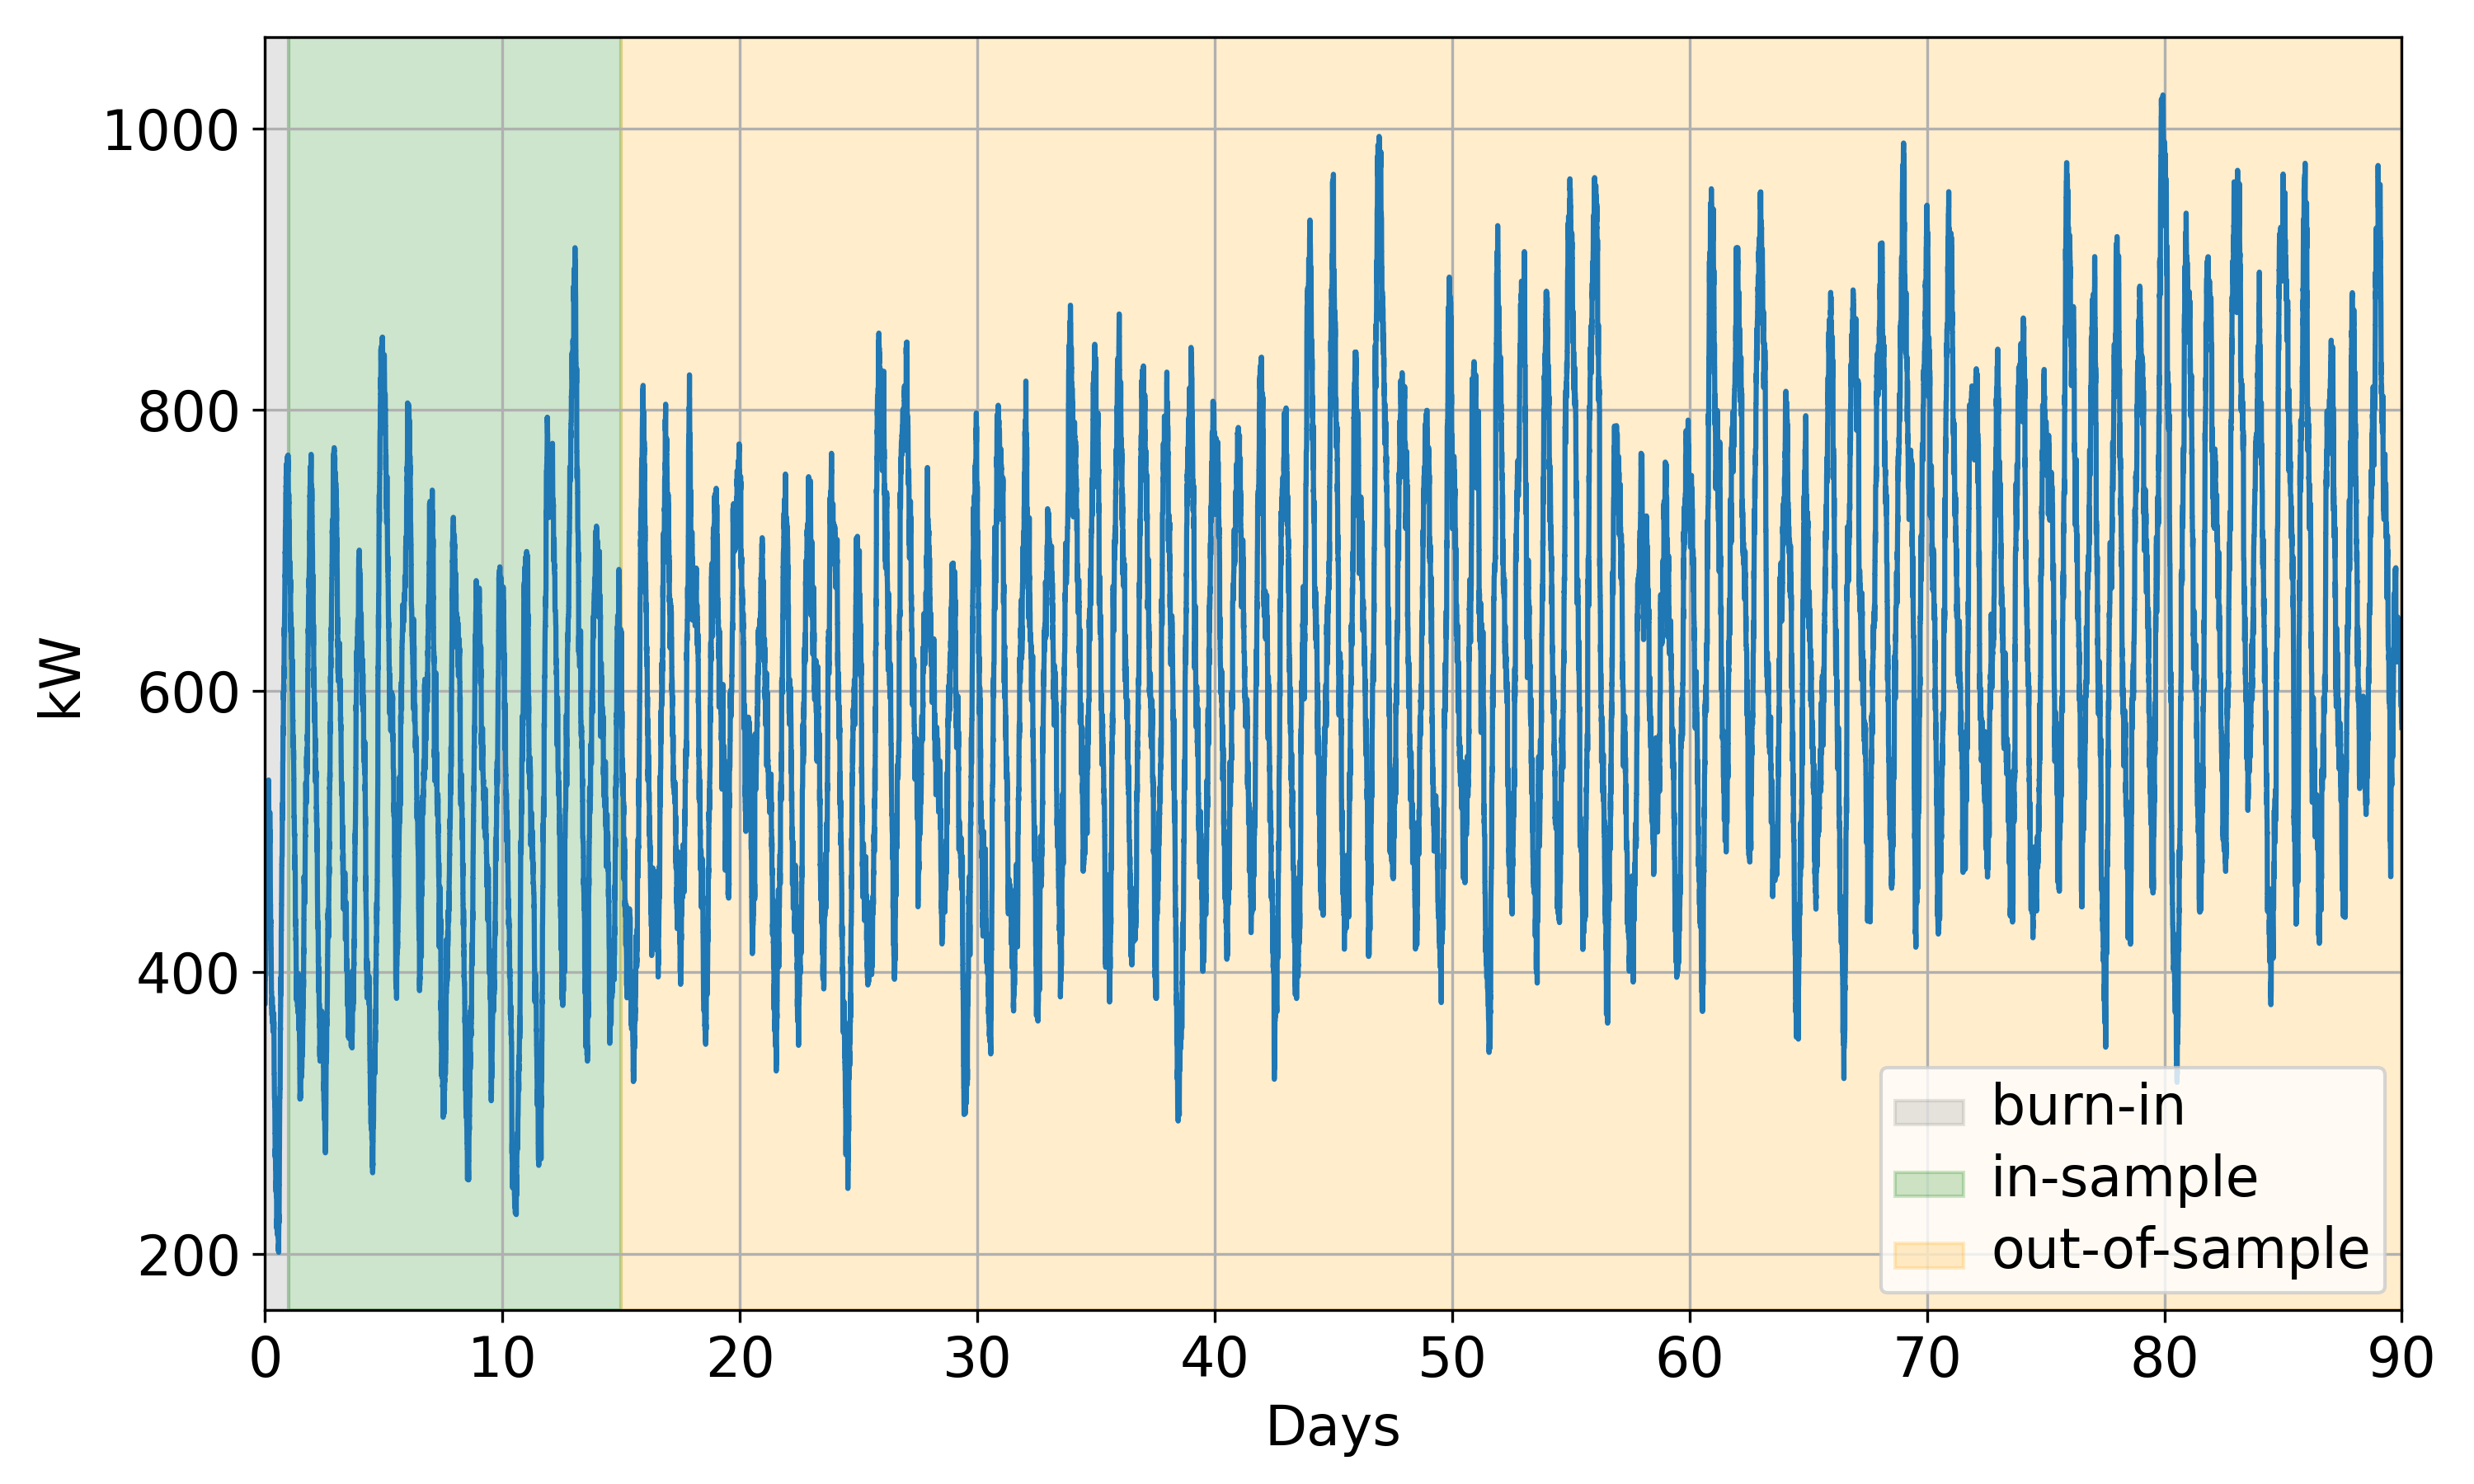
\includegraphics[width=\columnwidth]{../figures/drjcc_raw.png}
    \caption{Simulation of \ac{EV} power consumption for 90 days. First day is a burn-in period, green is the \ac{IS} period (corresponding to the empirical distribution), and yellow is the \ac{OOS} period.}
    \label{fig:drjcc_raw}
\end{figure}

The \ac{IS} period in Figure \ref{fig:drjcc_raw} thus defines the empirical distribution under which Problems \eqref{P90:General:DRJCC-tract} and \eqref{P90:TSO} are solved, and the bids are evaluated on the \ac{OOS} period. This is of course a stylized way of intentionally highlighting the efficacy of distributional robustness, but it generalizes to any situation where any flexible provider might have mis-specified its empirical (or predictive) distribution for any technology with stochastic baseline power.

\subsection{Aggregator bidding}

Figure \ref{fig:drjcc_bids} shows bids from an aggregator of 20 \acp{EV} and with $|\mathcal{I}| = 30$ with respect to their \ac{IS} available flexibility\footnote{We note that in this study, the uncertain future baseline power consumption corresponds to the available flexibility.} (as shown in blue) for different values of conservativeness $\theta$. Starting with the \ac{IS} period (left), all three bids are adhering to Definition \ref{def:P90}. For $\theta = 0.01$, the bids almost represent the 90\% quantile, i.e., the maximum allowed violation frequency. However, increasing $\theta$ decreases the bids (and therefore aggregator profits). But, as seen in the \ac{OOS} period (right), the bids for $\theta = 0.35$ are the only ones that (barely) adhere to the P90 rule. This is obviously due to the non-stationarity introduced as seen in Figure \ref{fig:drjcc_raw}.

Clearly, a low $\theta$ is risky in case the empirical distribution of available flexibility is just a little mis-specified. This might very well be the case for other technologies as well, e.g., for volatile wind and solar power production or other flexible demand prone to sudden disturbances. This highlights the awareness aggregators should have when bidding, but also how Definition \ref{def:P90} can be exploited to artificially allow for too high bids. This essentially corresponds to \textit{overfitting} to the empirical distribution, a term common in the machine learning literature \cite{bishop2006pattern}.

\begin{figure}[!t]
    \centering
    \begin{adjustbox}{width=\columnwidth}
        % This file was created with tikzplotlib v0.10.1.
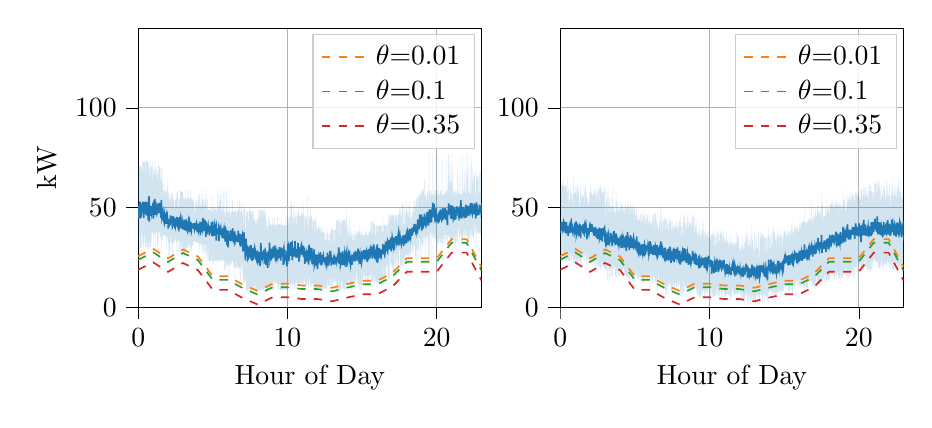
\begin{tikzpicture}

\definecolor{crimson2143940}{RGB}{214,39,40}
\definecolor{darkgray176}{RGB}{176,176,176}
\definecolor{darkorange25512714}{RGB}{255,127,14}
\definecolor{forestgreen4416044}{RGB}{44,160,44}
\definecolor{lightgray204}{RGB}{204,204,204}
\definecolor{steelblue31119180}{RGB}{31,119,180}

\begin{groupplot}[group style={group size=2 by 1}]
\nextgroupplot[
legend cell align={left},
legend style={fill opacity=0.8, draw opacity=1, text opacity=1, draw=lightgray204},
tick align=outside,
tick pos=left,
width=0.49\textwidth,
x grid style={darkgray176},
xlabel={Hour of Day},
xmajorgrids,
xmin=0, xmax=23,
xtick style={color=black},
y grid style={darkgray176},
ylabel={kW},
ymajorgrids,
ymin=0, ymax=139.944507818995,
ytick style={color=black}
]
\path [fill=steelblue31119180, fill opacity=0.2]
(axis cs:0,67.2360368810227)
--(axis cs:0,29.4917446709432)
--(axis cs:0.0166666666666667,29.4917446709432)
--(axis cs:0.0333333333333333,37.7026392795607)
--(axis cs:0.05,36.1543248766068)
--(axis cs:0.0666666666666667,22.2194952500217)
--(axis cs:0.0833333333333333,22.2194952500217)
--(axis cs:0.1,36.9623525900425)
--(axis cs:0.116666666666667,36.9623525900425)
--(axis cs:0.133333333333333,30.0705544461188)
--(axis cs:0.15,30.299772384379)
--(axis cs:0.166666666666667,28.0075930017773)
--(axis cs:0.183333333333333,28.0075930017773)
--(axis cs:0.2,36.9623525900425)
--(axis cs:0.216666666666667,28.0075930017773)
--(axis cs:0.233333333333333,37.7026392795607)
--(axis cs:0.25,43.3948640347184)
--(axis cs:0.266666666666667,39.6566914415438)
--(axis cs:0.283333333333333,28.0075930017773)
--(axis cs:0.3,38.7209995358274)
--(axis cs:0.316666666666667,36.9623525900425)
--(axis cs:0.333333333333333,30.299772384379)
--(axis cs:0.35,36.9623525900425)
--(axis cs:0.366666666666667,30.0705544461188)
--(axis cs:0.383333333333333,28.0075930017773)
--(axis cs:0.4,30.299772384379)
--(axis cs:0.416666666666667,37.7026392795607)
--(axis cs:0.433333333333333,36.7331346517824)
--(axis cs:0.45,36.9623525900425)
--(axis cs:0.466666666666667,30.299772384379)
--(axis cs:0.483333333333333,30.299772384379)
--(axis cs:0.5,30.299772384379)
--(axis cs:0.516666666666667,30.0705544461188)
--(axis cs:0.533333333333333,39.6566914415438)
--(axis cs:0.55,30.0705544461188)
--(axis cs:0.566666666666667,36.9623525900425)
--(axis cs:0.583333333333333,30.299772384379)
--(axis cs:0.6,28.0075930017773)
--(axis cs:0.616666666666667,39.9342371674162)
--(axis cs:0.633333333333333,30.299772384379)
--(axis cs:0.65,28.0075930017773)
--(axis cs:0.666666666666667,28.0075930017773)
--(axis cs:0.683333333333333,30.299772384379)
--(axis cs:0.7,28.0075930017773)
--(axis cs:0.716666666666667,39.6566914415438)
--(axis cs:0.733333333333333,28.0075930017773)
--(axis cs:0.75,30.0705544461188)
--(axis cs:0.766666666666667,37.7026392795607)
--(axis cs:0.783333333333333,30.0705544461188)
--(axis cs:0.8,30.299772384379)
--(axis cs:0.816666666666667,30.299772384379)
--(axis cs:0.833333333333333,30.299772384379)
--(axis cs:0.85,37.7026392795607)
--(axis cs:0.866666666666667,37.7026392795607)
--(axis cs:0.883333333333333,28.5690369733892)
--(axis cs:0.9,36.7892790489436)
--(axis cs:0.916666666666667,37.9148212030345)
--(axis cs:0.933333333333333,36.7892790489436)
--(axis cs:0.95,37.9148212030345)
--(axis cs:0.966666666666667,37.9148212030345)
--(axis cs:0.983333333333333,37.8936030106871)
--(axis cs:1,37.1015277682954)
--(axis cs:1.01666666666667,29.6756371286171)
--(axis cs:1.03333333333333,37.1015277682954)
--(axis cs:1.05,37.1015277682954)
--(axis cs:1.06666666666667,37.1015277682954)
--(axis cs:1.08333333333333,37.1015277682954)
--(axis cs:1.1,36.3589387043276)
--(axis cs:1.11666666666667,37.8936030106871)
--(axis cs:1.13333333333333,29.6756371286171)
--(axis cs:1.15,29.6756371286171)
--(axis cs:1.16666666666667,39.4470434672187)
--(axis cs:1.18333333333333,37.9148212030345)
--(axis cs:1.2,37.7026392795607)
--(axis cs:1.21666666666667,37.7026392795607)
--(axis cs:1.23333333333333,37.7026392795607)
--(axis cs:1.25,37.7026392795607)
--(axis cs:1.26666666666667,25.894025043117)
--(axis cs:1.28333333333333,25.894025043117)
--(axis cs:1.3,39.4470434672187)
--(axis cs:1.31666666666667,36.5217778559163)
--(axis cs:1.33333333333333,25.894025043117)
--(axis cs:1.35,37.8936030106871)
--(axis cs:1.36666666666667,37.7026392795607)
--(axis cs:1.38333333333333,37.7026392795607)
--(axis cs:1.4,37.7026392795607)
--(axis cs:1.41666666666667,37.8936030106871)
--(axis cs:1.43333333333333,37.8936030106871)
--(axis cs:1.45,34.0622068895613)
--(axis cs:1.46666666666667,37.9148212030345)
--(axis cs:1.48333333333333,37.9148212030345)
--(axis cs:1.5,33.2453887049169)
--(axis cs:1.51666666666667,36.4109976020351)
--(axis cs:1.53333333333333,32.3685988582758)
--(axis cs:1.55,39.9587467145356)
--(axis cs:1.56666666666667,29.3920271357896)
--(axis cs:1.58333333333333,29.3920271357896)
--(axis cs:1.6,29.7806940349754)
--(axis cs:1.61666666666667,35.9828463165765)
--(axis cs:1.63333333333333,35.9828463165765)
--(axis cs:1.65,36.6719743478656)
--(axis cs:1.66666666666667,35.5941794173907)
--(axis cs:1.68333333333333,35.1901317247859)
--(axis cs:1.7,36.2230324671935)
--(axis cs:1.71666666666667,36.6719743478656)
--(axis cs:1.73333333333333,36.2230324671935)
--(axis cs:1.75,36.6719743478656)
--(axis cs:1.76666666666667,36.2230324671935)
--(axis cs:1.78333333333333,36.2230324671935)
--(axis cs:1.8,35.1901317247859)
--(axis cs:1.81666666666667,35.1901317247859)
--(axis cs:1.83333333333333,36.2230324671935)
--(axis cs:1.85,35.1901317247859)
--(axis cs:1.86666666666667,36.6719743478656)
--(axis cs:1.88333333333333,25.894025043117)
--(axis cs:1.9,37.7821115232653)
--(axis cs:1.91666666666667,36.2230324671935)
--(axis cs:1.93333333333333,35.9243123120131)
--(axis cs:1.95,33.2358309153895)
--(axis cs:1.96666666666667,36.7492107808576)
--(axis cs:1.98333333333333,36.2230324671935)
--(axis cs:2,33.2358309153895)
--(axis cs:2.01666666666667,21.6662553429586)
--(axis cs:2.03333333333333,36.2230324671935)
--(axis cs:2.05,32.0788733581464)
--(axis cs:2.06666666666667,37.8233303679449)
--(axis cs:2.08333333333333,21.6662553429586)
--(axis cs:2.1,32.0788733581464)
--(axis cs:2.11666666666667,33.2358309153895)
--(axis cs:2.13333333333333,24.6347017926798)
--(axis cs:2.15,33.2358309153895)
--(axis cs:2.16666666666667,35.9243123120131)
--(axis cs:2.18333333333333,36.2230324671935)
--(axis cs:2.2,32.3757180031185)
--(axis cs:2.21666666666667,36.2230324671935)
--(axis cs:2.23333333333333,32.3757180031185)
--(axis cs:2.25,35.9243123120131)
--(axis cs:2.26666666666667,24.6347017926798)
--(axis cs:2.28333333333333,24.6347017926798)
--(axis cs:2.3,24.6347017926798)
--(axis cs:2.31666666666667,35.9243123120131)
--(axis cs:2.33333333333333,31.8792698468649)
--(axis cs:2.35,33.2358309153895)
--(axis cs:2.36666666666667,31.8792698468649)
--(axis cs:2.38333333333333,33.100174808537)
--(axis cs:2.4,35.3029894109232)
--(axis cs:2.41666666666667,31.8792698468649)
--(axis cs:2.43333333333333,38.0245027482229)
--(axis cs:2.45,33.2358309153895)
--(axis cs:2.46666666666667,35.5326736882047)
--(axis cs:2.48333333333333,35.3029894109232)
--(axis cs:2.5,32.6774855741525)
--(axis cs:2.51666666666667,35.9243123120131)
--(axis cs:2.53333333333333,33.2358309153895)
--(axis cs:2.55,32.6774855741525)
--(axis cs:2.56666666666667,33.2358309153895)
--(axis cs:2.58333333333333,27.6523775030204)
--(axis cs:2.6,33.2358309153895)
--(axis cs:2.61666666666667,33.2358309153895)
--(axis cs:2.63333333333333,33.2358309153895)
--(axis cs:2.65,27.6523775030204)
--(axis cs:2.66666666666667,27.6523775030204)
--(axis cs:2.68333333333333,27.6523775030204)
--(axis cs:2.7,35.3029894109232)
--(axis cs:2.71666666666667,35.5326736882047)
--(axis cs:2.73333333333333,33.2358309153895)
--(axis cs:2.75,27.6523775030204)
--(axis cs:2.76666666666667,35.3029894109232)
--(axis cs:2.78333333333333,33.2358309153895)
--(axis cs:2.8,32.9438524496541)
--(axis cs:2.81666666666667,28.4031511522827)
--(axis cs:2.83333333333333,25.5629684802893)
--(axis cs:2.85,27.6523775030204)
--(axis cs:2.86666666666667,36.1539965892946)
--(axis cs:2.88333333333333,32.4685446718794)
--(axis cs:2.9,32.4685446718794)
--(axis cs:2.91666666666667,25.5629684802893)
--(axis cs:2.93333333333333,25.5629684802893)
--(axis cs:2.95,27.6523775030204)
--(axis cs:2.96666666666667,27.4434366007473)
--(axis cs:2.98333333333333,25.5629684802893)
--(axis cs:3,27.4434366007473)
--(axis cs:3.01666666666667,27.6523775030204)
--(axis cs:3.03333333333333,27.6523775030204)
--(axis cs:3.05,27.6523775030204)
--(axis cs:3.06666666666667,27.4434366007473)
--(axis cs:3.08333333333333,27.6523775030204)
--(axis cs:3.1,25.5629684802893)
--(axis cs:3.11666666666667,32.8591060888288)
--(axis cs:3.13333333333333,27.6523775030204)
--(axis cs:3.15,27.6523775030204)
--(axis cs:3.16666666666667,27.6523775030204)
--(axis cs:3.18333333333333,27.4434366007473)
--(axis cs:3.2,25.5629684802893)
--(axis cs:3.21666666666667,32.8591060888288)
--(axis cs:3.23333333333333,29.9369253682925)
--(axis cs:3.25,29.9369253682925)
--(axis cs:3.26666666666667,29.9369253682925)
--(axis cs:3.28333333333333,32.5668880167751)
--(axis cs:3.3,27.6523775030204)
--(axis cs:3.31666666666667,32.5668880167751)
--(axis cs:3.33333333333333,29.9369253682925)
--(axis cs:3.35,33.2358309153895)
--(axis cs:3.36666666666667,32.9059403606798)
--(axis cs:3.38333333333333,29.9369253682925)
--(axis cs:3.4,32.8591060888288)
--(axis cs:3.41666666666667,32.5668880167751)
--(axis cs:3.43333333333333,27.6523775030204)
--(axis cs:3.45,32.8591060888288)
--(axis cs:3.46666666666667,29.9369253682925)
--(axis cs:3.48333333333333,29.7084705817653)
--(axis cs:3.5,29.9369253682925)
--(axis cs:3.51666666666667,29.9369253682925)
--(axis cs:3.53333333333333,30.8027176707672)
--(axis cs:3.55,27.6523775030204)
--(axis cs:3.56666666666667,33.1981584327334)
--(axis cs:3.58333333333333,27.6523775030204)
--(axis cs:3.6,32.8591060888288)
--(axis cs:3.61666666666667,32.8591060888288)
--(axis cs:3.63333333333333,30.8027176707672)
--(axis cs:3.65,32.6534672470226)
--(axis cs:3.66666666666667,30.8027176707672)
--(axis cs:3.68333333333333,33.1981584327334)
--(axis cs:3.7,30.8027176707672)
--(axis cs:3.71666666666667,33.1981584327334)
--(axis cs:3.73333333333333,33.2358309153895)
--(axis cs:3.75,33.785120355919)
--(axis cs:3.76666666666667,32.8591060888288)
--(axis cs:3.78333333333333,33.2358309153895)
--(axis cs:3.8,33.8461525159779)
--(axis cs:3.81666666666667,32.718968592354)
--(axis cs:3.83333333333333,32.718968592354)
--(axis cs:3.85,32.718968592354)
--(axis cs:3.86666666666667,34.1193302793675)
--(axis cs:3.88333333333333,32.450075934944)
--(axis cs:3.9,32.5603364694844)
--(axis cs:3.91666666666667,32.8591060888288)
--(axis cs:3.93333333333333,32.8292291268943)
--(axis cs:3.95,32.5603364694844)
--(axis cs:3.96666666666667,32.450075934944)
--(axis cs:3.98333333333333,32.8591060888288)
--(axis cs:4,31.4577311240813)
--(axis cs:4.01666666666667,33.747447873263)
--(axis cs:4.03333333333333,31.4577311240813)
--(axis cs:4.05,32.8591060888288)
--(axis cs:4.06666666666667,31.4577311240813)
--(axis cs:4.08333333333333,33.8461525159779)
--(axis cs:4.1,23.3593500468316)
--(axis cs:4.11666666666667,32.8591060888288)
--(axis cs:4.13333333333333,32.718968592354)
--(axis cs:4.15,31.4577311240813)
--(axis cs:4.16666666666667,32.718968592354)
--(axis cs:4.18333333333333,30.6478930163563)
--(axis cs:4.2,32.8591060888288)
--(axis cs:4.21666666666667,32.718968592354)
--(axis cs:4.23333333333333,31.4577311240813)
--(axis cs:4.25,32.718968592354)
--(axis cs:4.26666666666667,30.6478930163563)
--(axis cs:4.28333333333333,33.747447873263)
--(axis cs:4.3,23.3593500468316)
--(axis cs:4.31666666666667,31.4577311240813)
--(axis cs:4.33333333333333,30.6478930163563)
--(axis cs:4.35,32.8591060888288)
--(axis cs:4.36666666666667,23.3593500468316)
--(axis cs:4.38333333333333,31.4577311240813)
--(axis cs:4.4,31.4577311240813)
--(axis cs:4.41666666666667,31.4577311240813)
--(axis cs:4.43333333333333,23.3593500468316)
--(axis cs:4.45,32.8591060888288)
--(axis cs:4.46666666666667,31.4530101361516)
--(axis cs:4.48333333333333,31.4577311240813)
--(axis cs:4.5,31.4105212447841)
--(axis cs:4.51666666666667,31.0089429517335)
--(axis cs:4.53333333333333,23.3593500468316)
--(axis cs:4.55,31.4530101361516)
--(axis cs:4.56666666666667,23.3593500468316)
--(axis cs:4.58333333333333,31.0089429517335)
--(axis cs:4.6,26.9911994875335)
--(axis cs:4.61666666666667,23.3593500468316)
--(axis cs:4.63333333333333,23.3593500468316)
--(axis cs:4.65,34.7268635785548)
--(axis cs:4.66666666666667,27.0801853747429)
--(axis cs:4.68333333333333,34.6378776913453)
--(axis cs:4.7,24.1602230317169)
--(axis cs:4.71666666666667,23.3593500468316)
--(axis cs:4.73333333333333,24.2492089189263)
--(axis cs:4.75,23.3593500468316)
--(axis cs:4.76666666666667,23.3593500468316)
--(axis cs:4.78333333333333,24.2492089189263)
--(axis cs:4.8,22.024516215805)
--(axis cs:4.81666666666667,23.3593500468316)
--(axis cs:4.83333333333333,23.3593500468316)
--(axis cs:4.85,23.3593500468316)
--(axis cs:4.86666666666667,23.3593500468316)
--(axis cs:4.88333333333333,23.3593500468316)
--(axis cs:4.9,23.3593500468316)
--(axis cs:4.91666666666667,30.2154351190464)
--(axis cs:4.93333333333333,23.225866663729)
--(axis cs:4.95,22.024516215805)
--(axis cs:4.96666666666667,22.024516215805)
--(axis cs:4.98333333333333,24.1602230317169)
--(axis cs:5,24.1602230317169)
--(axis cs:5.01666666666667,22.024516215805)
--(axis cs:5.03333333333333,23.3593500468316)
--(axis cs:5.05,22.024516215805)
--(axis cs:5.06666666666667,24.1602230317169)
--(axis cs:5.08333333333333,23.3593500468316)
--(axis cs:5.1,23.3593500468316)
--(axis cs:5.11666666666667,23.3593500468316)
--(axis cs:5.13333333333333,24.0267396486142)
--(axis cs:5.15,23.225866663729)
--(axis cs:5.16666666666667,23.3593500468316)
--(axis cs:5.18333333333333,23.3593500468316)
--(axis cs:5.2,24.1602230317169)
--(axis cs:5.21666666666667,25.5881611001437)
--(axis cs:5.23333333333333,23.225866663729)
--(axis cs:5.25,22.024516215805)
--(axis cs:5.26666666666667,23.3593500468316)
--(axis cs:5.28333333333333,24.2492089189263)
--(axis cs:5.3,23.225866663729)
--(axis cs:5.31666666666667,23.225866663729)
--(axis cs:5.33333333333333,22.024516215805)
--(axis cs:5.35,23.3593500468316)
--(axis cs:5.36666666666667,24.0267396486142)
--(axis cs:5.38333333333333,24.2492089189263)
--(axis cs:5.4,23.225866663729)
--(axis cs:5.41666666666667,23.3593500468316)
--(axis cs:5.43333333333333,23.3593500468316)
--(axis cs:5.45,24.2492089189263)
--(axis cs:5.46666666666667,22.024516215805)
--(axis cs:5.48333333333333,23.3593500468316)
--(axis cs:5.5,23.3593500468316)
--(axis cs:5.51666666666667,24.1602230317169)
--(axis cs:5.53333333333333,24.2492089189263)
--(axis cs:5.55,23.3593500468316)
--(axis cs:5.56666666666667,23.3593500468316)
--(axis cs:5.58333333333333,24.1602230317169)
--(axis cs:5.6,23.3593500468316)
--(axis cs:5.61666666666667,23.3593500468316)
--(axis cs:5.63333333333333,23.225866663729)
--(axis cs:5.65,24.2492089189263)
--(axis cs:5.66666666666667,23.3593500468316)
--(axis cs:5.68333333333333,22.024516215805)
--(axis cs:5.7,23.3593500468316)
--(axis cs:5.71666666666667,24.1602230317169)
--(axis cs:5.73333333333333,25.5881611001437)
--(axis cs:5.75,23.225866663729)
--(axis cs:5.76666666666667,23.3593500468316)
--(axis cs:5.78333333333333,16.9523046469496)
--(axis cs:5.8,23.225866663729)
--(axis cs:5.81666666666667,16.9523046469496)
--(axis cs:5.83333333333333,22.024516215805)
--(axis cs:5.85,23.225866663729)
--(axis cs:5.86666666666667,19.1535744277441)
--(axis cs:5.88333333333333,23.225866663729)
--(axis cs:5.9,22.024516215805)
--(axis cs:5.91666666666667,24.0267396486142)
--(axis cs:5.93333333333333,19.1535744277441)
--(axis cs:5.95,22.024516215805)
--(axis cs:5.96666666666667,21.0312119365733)
--(axis cs:5.98333333333333,21.0312119365733)
--(axis cs:6,22.024516215805)
--(axis cs:6.01666666666667,21.0312119365733)
--(axis cs:6.03333333333333,12.0914734234885)
--(axis cs:6.05,22.024516215805)
--(axis cs:6.06666666666667,22.024516215805)
--(axis cs:6.08333333333333,21.0312119365733)
--(axis cs:6.1,22.024516215805)
--(axis cs:6.11666666666667,23.225866663729)
--(axis cs:6.13333333333333,12.0914734234885)
--(axis cs:6.15,21.0312119365733)
--(axis cs:6.16666666666667,21.0312119365733)
--(axis cs:6.18333333333333,22.024516215805)
--(axis cs:6.2,23.3593500468316)
--(axis cs:6.21666666666667,23.225866663729)
--(axis cs:6.23333333333333,23.0334353693826)
--(axis cs:6.25,22.024516215805)
--(axis cs:6.26666666666667,21.0312119365733)
--(axis cs:6.28333333333333,29.9929658487343)
--(axis cs:6.3,23.3593500468316)
--(axis cs:6.31666666666667,23.225866663729)
--(axis cs:6.33333333333333,24.1602230317169)
--(axis cs:6.35,23.225866663729)
--(axis cs:6.36666666666667,21.0312119365733)
--(axis cs:6.38333333333333,23.225866663729)
--(axis cs:6.4,22.2325623844973)
--(axis cs:6.41666666666667,19.6067688413599)
--(axis cs:6.43333333333333,23.3593500468316)
--(axis cs:6.45,19.6067688413599)
--(axis cs:6.46666666666667,23.3593500468316)
--(axis cs:6.48333333333333,12.0914734234885)
--(axis cs:6.5,19.6067688413599)
--(axis cs:6.51666666666667,20.4418016655678)
--(axis cs:6.53333333333333,20.4418016655678)
--(axis cs:6.55,20.4418016655678)
--(axis cs:6.56666666666667,19.6067688413599)
--(axis cs:6.58333333333333,23.0681992467017)
--(axis cs:6.6,23.3302349668186)
--(axis cs:6.61666666666667,20.4418016655678)
--(axis cs:6.63333333333333,19.6067688413599)
--(axis cs:6.65,20.4234175523232)
--(axis cs:6.66666666666667,20.4418016655678)
--(axis cs:6.68333333333333,12.0914734234885)
--(axis cs:6.7,30.3513412322678)
--(axis cs:6.71666666666667,20.4418016655678)
--(axis cs:6.73333333333333,20.2579605331211)
--(axis cs:6.75,20.4418016655678)
--(axis cs:6.76666666666667,19.4413118221578)
--(axis cs:6.78333333333333,19.6067688413599)
--(axis cs:6.8,20.4234175523232)
--(axis cs:6.81666666666667,12.0914734234885)
--(axis cs:6.83333333333333,20.2579605331211)
--(axis cs:6.85,12.0914734234885)
--(axis cs:6.86666666666667,20.2579605331211)
--(axis cs:6.88333333333333,20.4234175523232)
--(axis cs:6.9,20.4234175523232)
--(axis cs:6.91666666666667,20.4234175523232)
--(axis cs:6.93333333333333,20.2579605331211)
--(axis cs:6.95,14.2913260246953)
--(axis cs:6.96666666666667,22.4995486749024)
--(axis cs:6.98333333333333,22.7486140239892)
--(axis cs:7,19.4413118221578)
--(axis cs:7.01666666666667,14.2913260246953)
--(axis cs:7.03333333333333,12.648510057156)
--(axis cs:7.05,12.0914734234885)
--(axis cs:7.06666666666667,12.648510057156)
--(axis cs:7.08333333333333,19.4130768481344)
--(axis cs:7.1,14.1270444279414)
--(axis cs:7.11666666666667,12.648510057156)
--(axis cs:7.13333333333333,14.0713407645746)
--(axis cs:7.15,12.0914734234885)
--(axis cs:7.16666666666667,12.0914734234885)
--(axis cs:7.18333333333333,12.0914734234885)
--(axis cs:7.2,11.7772828342865)
--(axis cs:7.21666666666667,17.1731243377292)
--(axis cs:7.23333333333333,8.94956753146855)
--(axis cs:7.25,7.98014290475649)
--(axis cs:7.26666666666667,8.94956753146855)
--(axis cs:7.28333333333333,7.98014290475649)
--(axis cs:7.3,8.85262506879734)
--(axis cs:7.31666666666667,8.85262506879734)
--(axis cs:7.33333333333333,8.94956753146855)
--(axis cs:7.35,7.98014290475649)
--(axis cs:7.36666666666667,8.94956753146855)
--(axis cs:7.38333333333333,7.98014290475649)
--(axis cs:7.4,11.7772828342865)
--(axis cs:7.41666666666667,8.94956753146855)
--(axis cs:7.43333333333333,8.85262506879734)
--(axis cs:7.45,11.7772828342865)
--(axis cs:7.46666666666667,8.94956753146855)
--(axis cs:7.48333333333333,12.5928063937893)
--(axis cs:7.5,12.5928063937893)
--(axis cs:7.51666666666667,7.98014290475649)
--(axis cs:7.53333333333333,8.94956753146855)
--(axis cs:7.55,11.7772828342865)
--(axis cs:7.56666666666667,8.94956753146855)
--(axis cs:7.58333333333333,8.94956753146855)
--(axis cs:7.6,7.98014290475649)
--(axis cs:7.61666666666667,7.98014290475649)
--(axis cs:7.63333333333333,11.7772828342865)
--(axis cs:7.65,8.94956753146855)
--(axis cs:7.66666666666667,12.648510057156)
--(axis cs:7.68333333333333,11.7772828342865)
--(axis cs:7.7,8.85262506879734)
--(axis cs:7.71666666666667,8.94956753146855)
--(axis cs:7.73333333333333,8.94956753146855)
--(axis cs:7.75,7.98014290475649)
--(axis cs:7.76666666666667,8.94956753146855)
--(axis cs:7.78333333333333,8.85262506879734)
--(axis cs:7.8,8.78967793533981)
--(axis cs:7.81666666666667,12.5928063937893)
--(axis cs:7.83333333333333,11.7612938746737)
--(axis cs:7.85,12.648510057156)
--(axis cs:7.86666666666667,8.70872443228148)
--(axis cs:7.88333333333333,7.98014290475649)
--(axis cs:7.9,8.70872443228148)
--(axis cs:7.91666666666667,10.0777655581706)
--(axis cs:7.93333333333333,7.98014290475649)
--(axis cs:7.95,8.78967793533981)
--(axis cs:7.96666666666667,8.78967793533981)
--(axis cs:7.98333333333333,8.70872443228148)
--(axis cs:8,12.0914734234885)
--(axis cs:8.01666666666667,8.78967793533981)
--(axis cs:8.03333333333333,7.98014290475649)
--(axis cs:8.05,10.3108347418833)
--(axis cs:8.06666666666667,8.70872443228148)
--(axis cs:8.08333333333333,8.70872443228148)
--(axis cs:8.1,8.70872443228148)
--(axis cs:8.11666666666667,8.78967793533981)
--(axis cs:8.13333333333333,8.70872443228148)
--(axis cs:8.15,8.78967793533981)
--(axis cs:8.16666666666667,7.98014290475649)
--(axis cs:8.18333333333333,7.6549986394811)
--(axis cs:8.2,8.568121321039)
--(axis cs:8.21666666666667,8.70872443228148)
--(axis cs:8.23333333333333,7.98014290475649)
--(axis cs:8.25,12.2844691795173)
--(axis cs:8.26666666666667,8.63345225618151)
--(axis cs:8.28333333333333,10.1430964933131)
--(axis cs:8.3,8.568121321039)
--(axis cs:8.31666666666667,10.3108347418833)
--(axis cs:8.33333333333333,8.568121321039)
--(axis cs:8.35,8.568121321039)
--(axis cs:8.36666666666667,8.63345225618151)
--(axis cs:8.38333333333333,8.63345225618151)
--(axis cs:8.4,7.98014290475649)
--(axis cs:8.41666666666667,7.98014290475649)
--(axis cs:8.43333333333333,10.3108347418833)
--(axis cs:8.45,10.3108347418833)
--(axis cs:8.46666666666667,10.1430964933131)
--(axis cs:8.48333333333333,8.63345225618151)
--(axis cs:8.5,10.1430964933131)
--(axis cs:8.51666666666667,10.1430964933131)
--(axis cs:8.53333333333333,13.2087393802349)
--(axis cs:8.55,8.63345225618151)
--(axis cs:8.56666666666667,7.98014290475649)
--(axis cs:8.58333333333333,8.63345225618151)
--(axis cs:8.6,8.63345225618151)
--(axis cs:8.61666666666667,8.35855086958254)
--(axis cs:8.63333333333333,10.3108347418833)
--(axis cs:8.65,8.63345225618151)
--(axis cs:8.66666666666667,8.35855086958254)
--(axis cs:8.68333333333333,8.35855086958254)
--(axis cs:8.7,8.63345225618151)
--(axis cs:8.71666666666667,8.60596211752161)
--(axis cs:8.73333333333333,10.1430964933131)
--(axis cs:8.75,8.35855086958254)
--(axis cs:8.76666666666667,10.1430964933131)
--(axis cs:8.78333333333333,8.63345225618151)
--(axis cs:8.8,13.2087393802349)
--(axis cs:8.81666666666667,10.3108347418833)
--(axis cs:8.83333333333333,8.63345225618151)
--(axis cs:8.85,8.60596211752161)
--(axis cs:8.86666666666667,8.35855086958254)
--(axis cs:8.88333333333333,8.60596211752161)
--(axis cs:8.9,8.60596211752161)
--(axis cs:8.91666666666667,13.0135109930048)
--(axis cs:8.93333333333333,8.63345225618151)
--(axis cs:8.95,13.2888237100968)
--(axis cs:8.96666666666667,15.4226628429333)
--(axis cs:8.98333333333333,8.63345225618151)
--(axis cs:9,13.8035105586078)
--(axis cs:9.01666666666667,13.2590145897053)
--(axis cs:9.03333333333333,8.63345225618151)
--(axis cs:9.05,13.2865047283652)
--(axis cs:9.06666666666667,8.63345225618151)
--(axis cs:9.08333333333333,8.60596211752161)
--(axis cs:9.1,12.9734047110754)
--(axis cs:9.11666666666667,12.0443950154042)
--(axis cs:9.13333333333333,12.9734047110754)
--(axis cs:9.15,12.8805037415083)
--(axis cs:9.16666666666667,12.9734047110754)
--(axis cs:9.18333333333333,12.0443950154042)
--(axis cs:9.2,12.8805037415083)
--(axis cs:9.21666666666667,8.63345225618151)
--(axis cs:9.23333333333333,12.9734047110754)
--(axis cs:9.25,12.9734047110754)
--(axis cs:9.26666666666667,11.7033007394819)
--(axis cs:9.28333333333333,12.539409465586)
--(axis cs:9.3,12.0443950154042)
--(axis cs:9.31666666666667,8.63345225618151)
--(axis cs:9.33333333333333,12.0443950154042)
--(axis cs:9.35,11.7033007394819)
--(axis cs:9.36666666666667,11.7033007394819)
--(axis cs:9.38333333333333,8.63345225618151)
--(axis cs:9.4,12.0443950154042)
--(axis cs:9.41666666666667,8.63345225618151)
--(axis cs:9.43333333333333,11.8829378635147)
--(axis cs:9.45,11.5579893027814)
--(axis cs:9.46666666666667,11.5344971646062)
--(axis cs:9.48333333333333,8.63345225618151)
--(axis cs:9.5,11.8829378635147)
--(axis cs:9.51666666666667,8.60996011800633)
--(axis cs:9.53333333333333,8.60996011800633)
--(axis cs:9.55,8.39853087442975)
--(axis cs:9.56666666666667,8.63345225618151)
--(axis cs:9.58333333333333,8.60996011800633)
--(axis cs:9.6,12.0282493002152)
--(axis cs:9.61666666666667,8.63345225618151)
--(axis cs:9.63333333333333,8.63345225618151)
--(axis cs:9.65,11.8829378635147)
--(axis cs:9.66666666666667,8.60996011800633)
--(axis cs:9.68333333333333,8.63345225618151)
--(axis cs:9.7,11.5579893027814)
--(axis cs:9.71666666666667,8.60996011800633)
--(axis cs:9.73333333333333,8.63345225618151)
--(axis cs:9.75,11.8829378635147)
--(axis cs:9.76666666666667,8.63345225618151)
--(axis cs:9.78333333333333,12.0282493002152)
--(axis cs:9.8,11.5579893027814)
--(axis cs:9.81666666666667,8.60996011800633)
--(axis cs:9.83333333333333,8.39853087442975)
--(axis cs:9.85,11.8829378635147)
--(axis cs:9.86666666666667,11.5344971646062)
--(axis cs:9.88333333333333,11.5579893027814)
--(axis cs:9.9,8.39853087442975)
--(axis cs:9.91666666666667,8.39853087442975)
--(axis cs:9.93333333333333,8.63345225618151)
--(axis cs:9.95,8.39853087442975)
--(axis cs:9.96666666666667,8.63345225618151)
--(axis cs:9.98333333333333,11.5579893027814)
--(axis cs:10,8.39853087442975)
--(axis cs:10.0166666666667,11.8829378635147)
--(axis cs:10.0333333333333,12.0282493002152)
--(axis cs:10.05,12.0282493002152)
--(axis cs:10.0666666666667,11.5344971646062)
--(axis cs:10.0833333333333,11.5344971646062)
--(axis cs:10.1,11.8829378635147)
--(axis cs:10.1166666666667,11.8829378635147)
--(axis cs:10.1333333333333,12.711487294508)
--(axis cs:10.15,12.7856086588529)
--(axis cs:10.1666666666667,11.8829378635147)
--(axis cs:10.1833333333333,8.39853087442975)
--(axis cs:10.2,11.5344971646062)
--(axis cs:10.2166666666667,12.0282493002152)
--(axis cs:10.2333333333333,8.39853087442975)
--(axis cs:10.25,11.5344971646062)
--(axis cs:10.2666666666667,12.0282493002152)
--(axis cs:10.2833333333333,12.0282493002152)
--(axis cs:10.3,11.8829378635147)
--(axis cs:10.3166666666667,8.39853087442975)
--(axis cs:10.3333333333333,11.8829378635147)
--(axis cs:10.35,11.8829378635147)
--(axis cs:10.3666666666667,11.5344971646062)
--(axis cs:10.3833333333333,11.8829378635147)
--(axis cs:10.4,11.8829378635147)
--(axis cs:10.4166666666667,12.0282493002152)
--(axis cs:10.4333333333333,11.5344971646062)
--(axis cs:10.45,12.0282493002152)
--(axis cs:10.4666666666667,8.39853087442975)
--(axis cs:10.4833333333333,8.39853087442975)
--(axis cs:10.5,12.5949967462494)
--(axis cs:10.5166666666667,8.39853087442975)
--(axis cs:10.5333333333333,11.8829378635147)
--(axis cs:10.55,12.0282493002152)
--(axis cs:10.5666666666667,12.0443950154042)
--(axis cs:10.5833333333333,11.5344971646062)
--(axis cs:10.6,12.0282493002152)
--(axis cs:10.6166666666667,12.5399365731649)
--(axis cs:10.6333333333333,13.4169748452884)
--(axis cs:10.65,12.0282493002152)
--(axis cs:10.6666666666667,11.8829378635147)
--(axis cs:10.6833333333333,12.0282493002152)
--(axis cs:10.7,12.0443950154042)
--(axis cs:10.7166666666667,12.0443950154042)
--(axis cs:10.7333333333333,12.0282493002152)
--(axis cs:10.75,11.8829378635147)
--(axis cs:10.7666666666667,11.8829378635147)
--(axis cs:10.7833333333333,12.0282493002152)
--(axis cs:10.8,11.8829378635147)
--(axis cs:10.8166666666667,12.0443950154042)
--(axis cs:10.8333333333333,11.7560138384262)
--(axis cs:10.85,13.5083057451817)
--(axis cs:10.8666666666667,12.0443950154042)
--(axis cs:10.8833333333333,13.3619146722039)
--(axis cs:10.9,12.0443950154042)
--(axis cs:10.9166666666667,11.7560138384262)
--(axis cs:10.9333333333333,13.5083057451817)
--(axis cs:10.95,13.5083057451817)
--(axis cs:10.9666666666667,11.7560138384262)
--(axis cs:10.9833333333333,11.7560138384262)
--(axis cs:11,12.0443950154042)
--(axis cs:11.0166666666667,9.16058324562402)
--(axis cs:11.0333333333333,16.8091484458892)
--(axis cs:11.05,9.16058324562402)
--(axis cs:11.0666666666667,13.3619146722039)
--(axis cs:11.0833333333333,17.0975296228672)
--(axis cs:11.1,11.7945928418351)
--(axis cs:11.1166666666667,18.8464673714007)
--(axis cs:11.1333333333333,13.5083057451817)
--(axis cs:11.15,13.3619146722039)
--(axis cs:11.1666666666667,9.54637327971365)
--(axis cs:11.1833333333333,10.9516232166614)
--(axis cs:11.2,13.5083057451817)
--(axis cs:11.2166666666667,9.54637327971365)
--(axis cs:11.2333333333333,10.8110982229666)
--(axis cs:11.25,9.54637327971365)
--(axis cs:11.2666666666667,10.9516232166614)
--(axis cs:11.2833333333333,10.9516232166614)
--(axis cs:11.3,10.9516232166614)
--(axis cs:11.3166666666667,10.9516232166614)
--(axis cs:11.3333333333333,13.2526374923296)
--(axis cs:11.35,13.5083057451817)
--(axis cs:11.3666666666667,13.5083057451817)
--(axis cs:11.3833333333333,10.9516232166614)
--(axis cs:11.4,10.9516232166614)
--(axis cs:11.4166666666667,9.54637327971365)
--(axis cs:11.4333333333333,9.54637327971365)
--(axis cs:11.45,16.2159077436373)
--(axis cs:11.4666666666667,18.9928584443784)
--(axis cs:11.4833333333333,10.8110982229666)
--(axis cs:11.5,10.8110982229666)
--(axis cs:11.5166666666667,10.8110982229666)
--(axis cs:11.5333333333333,9.54637327971365)
--(axis cs:11.55,10.8110982229666)
--(axis cs:11.5666666666667,13.2526374923296)
--(axis cs:11.5833333333333,9.54637327971365)
--(axis cs:11.6,10.9516232166614)
--(axis cs:11.6166666666667,13.2526374923296)
--(axis cs:11.6333333333333,13.2526374923296)
--(axis cs:11.65,9.54637327971365)
--(axis cs:11.6666666666667,13.5083057451817)
--(axis cs:11.6833333333333,10.8110982229666)
--(axis cs:11.7,15.9602394907853)
--(axis cs:11.7166666666667,9.3405979284176)
--(axis cs:11.7333333333333,16.2159077436373)
--(axis cs:11.75,9.3405979284176)
--(axis cs:11.7666666666667,9.54637327971365)
--(axis cs:11.7833333333333,13.5083057451817)
--(axis cs:11.8,9.54637327971365)
--(axis cs:11.8166666666667,7.48861976675316)
--(axis cs:11.8333333333333,9.3405979284176)
--(axis cs:11.85,9.3405979284176)
--(axis cs:11.8666666666667,9.54637327971365)
--(axis cs:11.8833333333333,7.48861976675316)
--(axis cs:11.9,7.48861976675316)
--(axis cs:11.9166666666667,13.1121124986349)
--(axis cs:11.9333333333333,7.48861976675316)
--(axis cs:11.95,9.54637327971365)
--(axis cs:11.9666666666667,9.54637327971365)
--(axis cs:11.9833333333333,9.54637327971365)
--(axis cs:12,7.48861976675316)
--(axis cs:12.0166666666667,9.54637327971365)
--(axis cs:12.0333333333333,9.54637327971365)
--(axis cs:12.05,7.48861976675316)
--(axis cs:12.0666666666667,7.48861976675316)
--(axis cs:12.0833333333333,9.54637327971365)
--(axis cs:12.1,9.54637327971365)
--(axis cs:12.1166666666667,10.1893321527151)
--(axis cs:12.1333333333333,9.3405979284176)
--(axis cs:12.15,10.986692766188)
--(axis cs:12.1666666666667,9.3405979284176)
--(axis cs:12.1833333333333,10.8426608175406)
--(axis cs:12.2,9.54637327971365)
--(axis cs:12.2166666666667,10.986692766188)
--(axis cs:12.2333333333333,7.48861976675316)
--(axis cs:12.25,7.48861976675316)
--(axis cs:12.2666666666667,10.8426608175406)
--(axis cs:12.2833333333333,7.48861976675316)
--(axis cs:12.3,9.54637327971365)
--(axis cs:12.3166666666667,9.54637327971365)
--(axis cs:12.3333333333333,9.3405979284176)
--(axis cs:12.35,9.54637327971365)
--(axis cs:12.3666666666667,9.3405979284176)
--(axis cs:12.3833333333333,10.8426608175406)
--(axis cs:12.4,9.3405979284176)
--(axis cs:12.4166666666667,7.48861976675316)
--(axis cs:12.4333333333333,10.986692766188)
--(axis cs:12.45,10.8426608175406)
--(axis cs:12.4666666666667,9.3405979284176)
--(axis cs:12.4833333333333,9.3405979284176)
--(axis cs:12.5,9.54637327971365)
--(axis cs:12.5166666666667,9.54637327971365)
--(axis cs:12.5333333333333,9.54637327971365)
--(axis cs:12.55,9.3405979284176)
--(axis cs:12.5666666666667,9.54637327971365)
--(axis cs:12.5833333333333,7.48861976675316)
--(axis cs:12.6,10.986692766188)
--(axis cs:12.6166666666667,9.54637327971365)
--(axis cs:12.6333333333333,9.3405979284176)
--(axis cs:12.65,9.3405979284176)
--(axis cs:12.6666666666667,9.54637327971365)
--(axis cs:12.6833333333333,14.1953364264848)
--(axis cs:12.7,14.55185238874)
--(axis cs:12.7166666666667,10.8426608175406)
--(axis cs:12.7333333333333,10.986692766188)
--(axis cs:12.75,16.1524268445562)
--(axis cs:12.7666666666667,9.54637327971365)
--(axis cs:12.7833333333333,10.8426608175406)
--(axis cs:12.8,10.8426608175406)
--(axis cs:12.8166666666667,10.986692766188)
--(axis cs:12.8333333333333,10.8426608175406)
--(axis cs:12.85,10.8426608175406)
--(axis cs:12.8666666666667,10.986692766188)
--(axis cs:12.8833333333333,10.8426608175406)
--(axis cs:12.9,14.1953364264848)
--(axis cs:12.9166666666667,14.1953364264848)
--(axis cs:12.9333333333333,14.1953364264848)
--(axis cs:12.95,9.54637327971365)
--(axis cs:12.9666666666667,10.8426608175406)
--(axis cs:12.9833333333333,10.986692766188)
--(axis cs:13,13.0546039219083)
--(axis cs:13.0166666666667,9.54637327971365)
--(axis cs:13.0333333333333,9.54637327971365)
--(axis cs:13.05,14.4021275420568)
--(axis cs:13.0666666666667,13.0546039219083)
--(axis cs:13.0833333333333,14.55185238874)
--(axis cs:13.1,14.4021275420568)
--(axis cs:13.1166666666667,13.0546039219083)
--(axis cs:13.1333333333333,12.3826312841683)
--(axis cs:13.15,14.55185238874)
--(axis cs:13.1666666666667,12.3826312841683)
--(axis cs:13.1833333333333,14.55185238874)
--(axis cs:13.2,14.4021275420568)
--(axis cs:13.2166666666667,12.3826312841683)
--(axis cs:13.2333333333333,13.0546039219083)
--(axis cs:13.25,13.0546039219083)
--(axis cs:13.2666666666667,12.3826312841683)
--(axis cs:13.2833333333333,8.32399101069401)
--(axis cs:13.3,13.9290662509354)
--(axis cs:13.3166666666667,6.33487754450831)
--(axis cs:13.3333333333333,6.33487754450831)
--(axis cs:13.35,8.12507966407544)
--(axis cs:13.3666666666667,19.7354451506645)
--(axis cs:13.3833333333333,8.12507966407544)
--(axis cs:13.4,8.12507966407544)
--(axis cs:13.4166666666667,6.33487754450831)
--(axis cs:13.4333333333333,14.55185238874)
--(axis cs:13.45,13.7301549043168)
--(axis cs:13.4666666666667,8.32399101069401)
--(axis cs:13.4833333333333,8.32399101069401)
--(axis cs:13.5,8.12507966407544)
--(axis cs:13.5166666666667,8.32399101069401)
--(axis cs:13.5333333333333,13.9290662509354)
--(axis cs:13.55,8.21469797096329)
--(axis cs:13.5666666666667,8.32399101069401)
--(axis cs:13.5833333333333,14.55185238874)
--(axis cs:13.6,13.9290662509354)
--(axis cs:13.6166666666667,13.9290662509354)
--(axis cs:13.6333333333333,8.31306170672094)
--(axis cs:13.65,8.32399101069401)
--(axis cs:13.6666666666667,8.31306170672094)
--(axis cs:13.6833333333333,16.0980528865696)
--(axis cs:13.7,13.9290662509354)
--(axis cs:13.7166666666667,8.21469797096329)
--(axis cs:13.7333333333333,8.32399101069401)
--(axis cs:13.75,13.9290662509354)
--(axis cs:13.7666666666667,8.31306170672094)
--(axis cs:13.7833333333333,15.8213386334266)
--(axis cs:13.8,8.21469797096329)
--(axis cs:13.8166666666667,8.21469797096329)
--(axis cs:13.8333333333333,8.32399101069401)
--(axis cs:13.85,11.78470985731)
--(axis cs:13.8666666666667,11.4386379726484)
--(axis cs:13.8833333333333,11.4386379726484)
--(axis cs:13.9,8.31306170672094)
--(axis cs:13.9166666666667,11.78470985731)
--(axis cs:13.9333333333333,8.32399101069401)
--(axis cs:13.95,15.8213386334266)
--(axis cs:13.9666666666667,11.78470985731)
--(axis cs:13.9833333333333,11.78470985731)
--(axis cs:14,11.78470985731)
--(axis cs:14.0166666666667,11.78470985731)
--(axis cs:14.0333333333333,8.21469797096329)
--(axis cs:14.05,13.676008989306)
--(axis cs:14.0666666666667,13.4868790761064)
--(axis cs:14.0833333333333,13.4868790761064)
--(axis cs:14.1,16.0104685466262)
--(axis cs:14.1166666666667,11.78470985731)
--(axis cs:14.1333333333333,11.78470985731)
--(axis cs:14.15,11.78470985731)
--(axis cs:14.1666666666667,8.21469797096329)
--(axis cs:14.1833333333333,11.4277086686753)
--(axis cs:14.2,8.21469797096329)
--(axis cs:14.2166666666667,11.4277086686753)
--(axis cs:14.2333333333333,11.78470985731)
--(axis cs:14.25,11.4277086686753)
--(axis cs:14.2666666666667,8.21469797096329)
--(axis cs:14.2833333333333,8.21469797096329)
--(axis cs:14.3,11.4277086686753)
--(axis cs:14.3166666666667,11.4277086686753)
--(axis cs:14.3333333333333,8.21469797096329)
--(axis cs:14.35,11.4277086686753)
--(axis cs:14.3666666666667,11.78470985731)
--(axis cs:14.3833333333333,11.78470985731)
--(axis cs:14.4,15.8213386334266)
--(axis cs:14.4166666666667,16.269852941884)
--(axis cs:14.4333333333333,16.269852941884)
--(axis cs:14.45,8.21469797096329)
--(axis cs:14.4666666666667,22.0201004250567)
--(axis cs:14.4833333333333,11.4277086686753)
--(axis cs:14.5,8.21469797096329)
--(axis cs:14.5166666666667,15.8213386334266)
--(axis cs:14.5333333333333,11.78470985731)
--(axis cs:14.55,11.78470985731)
--(axis cs:14.5666666666667,15.8213386334266)
--(axis cs:14.5833333333333,9.35238742297895)
--(axis cs:14.6,16.269852941884)
--(axis cs:14.6166666666667,20.1269029548978)
--(axis cs:14.6333333333333,16.269852941884)
--(axis cs:14.65,16.0471006371502)
--(axis cs:14.6666666666667,13.5859766413004)
--(axis cs:14.6833333333333,9.4787973620918)
--(axis cs:14.7,13.5859766413004)
--(axis cs:14.7166666666667,13.5859766413004)
--(axis cs:14.7333333333333,16.0471006371502)
--(axis cs:14.75,9.4787973620918)
--(axis cs:14.7666666666667,9.4787973620918)
--(axis cs:14.7833333333333,13.5859766413004)
--(axis cs:14.8,9.4787973620918)
--(axis cs:14.8166666666667,14.0423298945458)
--(axis cs:14.8333333333333,8.21469797096329)
--(axis cs:14.85,9.35238742297895)
--(axis cs:14.8666666666667,13.5859766413004)
--(axis cs:14.8833333333333,8.21469797096329)
--(axis cs:14.9,9.4787973620918)
--(axis cs:14.9166666666667,13.5859766413004)
--(axis cs:14.9333333333333,9.4787973620918)
--(axis cs:14.95,9.4787973620918)
--(axis cs:14.9666666666667,8.21469797096329)
--(axis cs:14.9833333333333,9.35238742297895)
--(axis cs:15,16.2076029772048)
--(axis cs:15.0166666666667,16.2636279454161)
--(axis cs:15.0333333333333,14.1875567721565)
--(axis cs:15.05,11.7421820645102)
--(axis cs:15.0666666666667,14.4592650730061)
--(axis cs:15.0833333333333,14.4592650730061)
--(axis cs:15.1,14.1875567721565)
--(axis cs:15.1166666666667,20.4723297625329)
--(axis cs:15.1333333333333,16.1900004839958)
--(axis cs:15.15,16.1900004839958)
--(axis cs:15.1666666666667,15.7452186420473)
--(axis cs:15.1833333333333,16.1900004839958)
--(axis cs:15.2,11.7421820645102)
--(axis cs:15.2166666666667,16.2636279454161)
--(axis cs:15.2333333333333,16.2058427278839)
--(axis cs:15.25,11.7421820645102)
--(axis cs:15.2666666666667,16.2076029772048)
--(axis cs:15.2833333333333,16.269852941884)
--(axis cs:15.3,15.7610608859354)
--(axis cs:15.3166666666667,15.8170858541466)
--(axis cs:15.3333333333333,16.2076029772048)
--(axis cs:15.35,11.7421820645102)
--(axis cs:15.3666666666667,16.2076029772048)
--(axis cs:15.3833333333333,11.7421820645102)
--(axis cs:15.4,16.2636279454161)
--(axis cs:15.4166666666667,11.7421820645102)
--(axis cs:15.4333333333333,16.269852941884)
--(axis cs:15.45,16.2076029772048)
--(axis cs:15.4666666666667,16.269852941884)
--(axis cs:15.4833333333333,15.7610608859354)
--(axis cs:15.5,16.2076029772048)
--(axis cs:15.5166666666667,16.2076029772048)
--(axis cs:15.5333333333333,11.7421820645102)
--(axis cs:15.55,16.269852941884)
--(axis cs:15.5666666666667,15.7610608859354)
--(axis cs:15.5833333333333,16.2076029772048)
--(axis cs:15.6,21.4450756767394)
--(axis cs:15.6166666666667,15.8465022056743)
--(axis cs:15.6333333333333,12.5111539421605)
--(axis cs:15.65,12.5965952618994)
--(axis cs:15.6666666666667,15.8465022056743)
--(axis cs:15.6833333333333,11.7421820645102)
--(axis cs:15.7,11.7421820645102)
--(axis cs:15.7166666666667,15.7610608859354)
--(axis cs:15.7333333333333,12.5965952618994)
--(axis cs:15.75,12.5965952618994)
--(axis cs:15.7666666666667,15.8465022056743)
--(axis cs:15.7833333333333,15.8465022056743)
--(axis cs:15.8,16.2076029772048)
--(axis cs:15.8166666666667,12.5221978118117)
--(axis cs:15.8333333333333,11.8526207610221)
--(axis cs:15.85,12.5965952618994)
--(axis cs:15.8666666666667,15.8465022056743)
--(axis cs:15.8833333333333,15.8465022056743)
--(axis cs:15.9,11.8526207610221)
--(axis cs:15.9166666666667,16.2076029772048)
--(axis cs:15.9333333333333,12.5221978118117)
--(axis cs:15.95,12.5965952618994)
--(axis cs:15.9666666666667,12.5221978118117)
--(axis cs:15.9833333333333,11.8526207610221)
--(axis cs:16,9.87272543269653)
--(axis cs:16.0166666666667,21.1974832443967)
--(axis cs:16.0333333333333,12.5965952618994)
--(axis cs:16.05,12.3242082789791)
--(axis cs:16.0666666666667,12.3242082789791)
--(axis cs:16.0833333333333,21.1974832443967)
--(axis cs:16.1,12.5965952618994)
--(axis cs:16.1166666666667,12.5965952618994)
--(axis cs:16.1333333333333,13.4274155888271)
--(axis cs:16.15,20.1025304497493)
--(axis cs:16.1666666666667,9.87272543269653)
--(axis cs:16.1833333333333,13.1550286059068)
--(axis cs:16.2,19.4442503006229)
--(axis cs:16.2166666666667,13.1550286059068)
--(axis cs:16.2333333333333,13.5197289584857)
--(axis cs:16.25,20.1025304497493)
--(axis cs:16.2666666666667,13.1550286059068)
--(axis cs:16.2833333333333,9.87272543269653)
--(axis cs:16.3,20.4297078158056)
--(axis cs:16.3166666666667,13.5197289584857)
--(axis cs:16.3333333333333,14.6042567441655)
--(axis cs:16.35,19.5527030791909)
--(axis cs:16.3666666666667,13.5197289584857)
--(axis cs:16.3833333333333,14.6042567441655)
--(axis cs:16.4,20.1025304497493)
--(axis cs:16.4166666666667,20.1025304497493)
--(axis cs:16.4333333333333,13.5197289584857)
--(axis cs:16.45,19.5527030791909)
--(axis cs:16.4666666666667,13.5197289584857)
--(axis cs:16.4833333333333,13.5197289584857)
--(axis cs:16.5,14.6042567441655)
--(axis cs:16.5166666666667,20.5381605943735)
--(axis cs:16.5333333333333,14.6042567441655)
--(axis cs:16.55,13.5197289584857)
--(axis cs:16.5666666666667,14.4958039655975)
--(axis cs:16.5833333333333,14.6042567441655)
--(axis cs:16.6,21.5527857277552)
--(axis cs:16.6166666666667,21.5527857277552)
--(axis cs:16.6333333333333,20.4297078158056)
--(axis cs:16.65,20.4297078158056)
--(axis cs:16.6666666666667,13.5197289584857)
--(axis cs:16.6833333333333,13.5197289584857)
--(axis cs:16.7,21.5172554794194)
--(axis cs:16.7166666666667,21.1974832443967)
--(axis cs:16.7333333333333,21.1974832443967)
--(axis cs:16.75,13.5197289584857)
--(axis cs:16.7666666666667,26.5349367246897)
--(axis cs:16.7833333333333,13.5197289584857)
--(axis cs:16.8,13.5197289584857)
--(axis cs:16.8166666666667,21.1974832443967)
--(axis cs:16.8333333333333,13.5197289584857)
--(axis cs:16.85,28.6876562923631)
--(axis cs:16.8666666666667,29.3347233779395)
--(axis cs:16.8833333333333,28.6876562923631)
--(axis cs:16.9,21.1974832443967)
--(axis cs:16.9166666666667,27.9386389875665)
--(axis cs:16.9333333333333,21.1974832443967)
--(axis cs:16.95,21.1974832443967)
--(axis cs:16.9666666666667,28.7057079947796)
--(axis cs:16.9833333333333,20.4297078158056)
--(axis cs:17,13.5197289584857)
--(axis cs:17.0166666666667,29.4066197207813)
--(axis cs:17.0333333333333,20.4297078158056)
--(axis cs:17.05,21.1974832443967)
--(axis cs:17.0666666666667,13.5197289584857)
--(axis cs:17.0833333333333,20.4297078158056)
--(axis cs:17.1,13.5197289584857)
--(axis cs:17.1166666666667,20.4297078158056)
--(axis cs:17.1333333333333,13.5197289584857)
--(axis cs:17.15,13.5197289584857)
--(axis cs:17.1666666666667,28.4788246252635)
--(axis cs:17.1833333333333,28.4788246252635)
--(axis cs:17.2,21.1974832443967)
--(axis cs:17.2166666666667,20.4297078158056)
--(axis cs:17.2333333333333,29.2878625564709)
--(axis cs:17.25,21.1974832443967)
--(axis cs:17.2666666666667,29.4066197207813)
--(axis cs:17.2833333333333,28.4788246252635)
--(axis cs:17.3,20.8754360161065)
--(axis cs:17.3166666666667,21.1974832443967)
--(axis cs:17.3333333333333,21.1974832443967)
--(axis cs:17.35,20.8754360161065)
--(axis cs:17.3666666666667,20.8754360161065)
--(axis cs:17.3833333333333,29.4394360875755)
--(axis cs:17.4,28.6152408032576)
--(axis cs:17.4166666666667,20.8754360161065)
--(axis cs:17.4333333333333,17.9770109614947)
--(axis cs:17.45,21.1974832443967)
--(axis cs:17.4666666666667,29.3947440043503)
--(axis cs:17.4833333333333,29.4066197207813)
--(axis cs:17.5,28.4788246252635)
--(axis cs:17.5166666666667,29.2878625564709)
--(axis cs:17.5333333333333,21.1974832443967)
--(axis cs:17.55,17.9770109614947)
--(axis cs:17.5666666666667,20.8754360161065)
--(axis cs:17.5833333333333,21.1974832443967)
--(axis cs:17.6,21.1974832443967)
--(axis cs:17.6166666666667,17.9770109614947)
--(axis cs:17.6333333333333,21.1974832443967)
--(axis cs:17.65,28.0713642917894)
--(axis cs:17.6666666666667,21.1974832443967)
--(axis cs:17.6833333333333,21.1974832443967)
--(axis cs:17.7,21.1974832443967)
--(axis cs:17.7166666666667,29.4147883894446)
--(axis cs:17.7333333333333,21.1974832443967)
--(axis cs:17.75,28.3934115200795)
--(axis cs:17.7666666666667,17.9770109614947)
--(axis cs:17.7833333333333,21.1974832443967)
--(axis cs:17.8,20.8754360161065)
--(axis cs:17.8166666666667,21.1974832443967)
--(axis cs:17.8333333333333,21.1974832443967)
--(axis cs:17.85,28.0516542923042)
--(axis cs:17.8666666666667,29.0788286248703)
--(axis cs:17.8833333333333,21.1974832443967)
--(axis cs:17.9,21.1974832443967)
--(axis cs:17.9166666666667,25.844649595237)
--(axis cs:17.9333333333333,26.361001411997)
--(axis cs:17.95,25.844649595237)
--(axis cs:17.9666666666667,27.8825890042735)
--(axis cs:17.9833333333333,27.8825890042735)
--(axis cs:18,21.1974832443967)
--(axis cs:18.0166666666667,25.844649595237)
--(axis cs:18.0333333333333,25.844649595237)
--(axis cs:18.05,26.361001411997)
--(axis cs:18.0666666666667,26.361001411997)
--(axis cs:18.0833333333333,26.361001411997)
--(axis cs:18.1,26.361001411997)
--(axis cs:18.1166666666667,26.361001411997)
--(axis cs:18.1333333333333,21.1974832443967)
--(axis cs:18.15,21.1974832443967)
--(axis cs:18.1666666666667,26.361001411997)
--(axis cs:18.1833333333333,27.8825890042735)
--(axis cs:18.2,28.0516542923042)
--(axis cs:18.2166666666667,27.8825890042735)
--(axis cs:18.2333333333333,28.0516542923042)
--(axis cs:18.25,21.1974832443967)
--(axis cs:18.2666666666667,26.361001411997)
--(axis cs:18.2833333333333,27.8825890042735)
--(axis cs:18.3,27.3662371875134)
--(axis cs:18.3166666666667,33.5925977041251)
--(axis cs:18.3333333333333,33.5091282944204)
--(axis cs:18.35,28.0516542923042)
--(axis cs:18.3666666666667,34.856298043486)
--(axis cs:18.3833333333333,21.1974832443967)
--(axis cs:18.4,35.0819031554313)
--(axis cs:18.4166666666667,34.1758336683679)
--(axis cs:18.4333333333333,34.1758336683679)
--(axis cs:18.45,28.0516542923042)
--(axis cs:18.4666666666667,28.0516542923042)
--(axis cs:18.4833333333333,33.4904165635771)
--(axis cs:18.5,35.0819031554313)
--(axis cs:18.5166666666667,27.3662371875134)
--(axis cs:18.5333333333333,34.856298043486)
--(axis cs:18.55,28.0516542923042)
--(axis cs:18.5666666666667,21.1974832443967)
--(axis cs:18.5833333333333,28.0516542923042)
--(axis cs:18.6,28.7177348408888)
--(axis cs:18.6166666666667,28.7177348408888)
--(axis cs:18.6333333333333,28.7177348408888)
--(axis cs:18.65,28.7177348408888)
--(axis cs:18.6666666666667,21.1974832443967)
--(axis cs:18.6833333333333,34.856298043486)
--(axis cs:18.7,21.1974832443967)
--(axis cs:18.7166666666667,33.4904165635771)
--(axis cs:18.7333333333333,35.716337944158)
--(axis cs:18.75,34.2424417232263)
--(axis cs:18.7666666666667,28.7177348408888)
--(axis cs:18.7833333333333,27.9657096812396)
--(axis cs:18.8,32.2187013541739)
--(axis cs:18.8166666666667,21.1974832443967)
--(axis cs:18.8333333333333,33.4432811441492)
--(axis cs:18.85,34.9180409543031)
--(axis cs:18.8666666666667,34.9180409543031)
--(axis cs:18.8833333333333,35.0819031554313)
--(axis cs:18.9,32.2187013541739)
--(axis cs:18.9166666666667,21.1974832443967)
--(axis cs:18.9333333333333,33.4432811441492)
--(axis cs:18.95,32.2187013541739)
--(axis cs:18.9666666666667,33.4432811441492)
--(axis cs:18.9833333333333,34.9180409543031)
--(axis cs:19,21.1974832443967)
--(axis cs:19.0166666666667,33.4432811441492)
--(axis cs:19.0333333333333,31.6144854515713)
--(axis cs:19.05,33.4432811441492)
--(axis cs:19.0666666666667,30.5727852308538)
--(axis cs:19.0833333333333,30.5727852308538)
--(axis cs:19.1,35.8525336144198)
--(axis cs:19.1166666666667,35.8118979331215)
--(axis cs:19.1333333333333,35.8118979331215)
--(axis cs:19.15,21.1974832443967)
--(axis cs:19.1666666666667,34.350456464249)
--(axis cs:19.1833333333333,36.302293643824)
--(axis cs:19.2,36.2982300756942)
--(axis cs:19.2166666666667,34.350456464249)
--(axis cs:19.2333333333333,35.8118979331215)
--(axis cs:19.25,34.350456464249)
--(axis cs:19.2666666666667,21.1974832443967)
--(axis cs:19.2833333333333,35.8118979331215)
--(axis cs:19.3,35.8118979331215)
--(axis cs:19.3166666666667,35.8118979331215)
--(axis cs:19.3333333333333,35.8118979331215)
--(axis cs:19.35,21.1974832443967)
--(axis cs:19.3666666666667,34.350456464249)
--(axis cs:19.3833333333333,36.2982300756942)
--(axis cs:19.4,36.4737972455551)
--(axis cs:19.4166666666667,35.8118979331215)
--(axis cs:19.4333333333333,34.350456464249)
--(axis cs:19.45,21.1974832443967)
--(axis cs:19.4666666666667,35.8118979331215)
--(axis cs:19.4833333333333,21.1974832443967)
--(axis cs:19.5,35.8118979331215)
--(axis cs:19.5166666666667,34.9583188719524)
--(axis cs:19.5333333333333,21.1974832443967)
--(axis cs:19.55,34.350456464249)
--(axis cs:19.5666666666667,36.4873006083474)
--(axis cs:19.5833333333333,36.4873006083474)
--(axis cs:19.6,38.3765280129976)
--(axis cs:19.6166666666667,37.3442562081063)
--(axis cs:19.6333333333333,38.2733008325085)
--(axis cs:19.65,21.1974832443967)
--(axis cs:19.6666666666667,36.4873006083474)
--(axis cs:19.6833333333333,36.4873006083474)
--(axis cs:19.7,34.9583188719524)
--(axis cs:19.7166666666667,37.3442562081063)
--(axis cs:19.7333333333333,38.2733008325085)
--(axis cs:19.75,21.1974832443967)
--(axis cs:19.7666666666667,38.1876052725326)
--(axis cs:19.7833333333333,36.4873006083474)
--(axis cs:19.8,34.9583188719524)
--(axis cs:19.8166666666667,37.2585606481304)
--(axis cs:19.8333333333333,36.4873006083474)
--(axis cs:19.85,34.6266864370862)
--(axis cs:19.8666666666667,33.2837661178172)
--(axis cs:19.8833333333333,33.2837661178172)
--(axis cs:19.9,34.9583188719524)
--(axis cs:19.9166666666667,34.6266864370862)
--(axis cs:19.9333333333333,34.6266864370862)
--(axis cs:19.95,36.3012391912213)
--(axis cs:19.9666666666667,34.6266864370862)
--(axis cs:19.9833333333333,21.1974832443967)
--(axis cs:20,30.4964126107777)
--(axis cs:20.0166666666667,30.4964126107777)
--(axis cs:20.0333333333333,21.1974832443967)
--(axis cs:20.05,32.4452230020958)
--(axis cs:20.0666666666667,31.5153300654577)
--(axis cs:20.0833333333333,35.3161977176671)
--(axis cs:20.1,32.66175749002)
--(axis cs:20.1166666666667,36.3012391912213)
--(axis cs:20.1333333333333,31.5153300654577)
--(axis cs:20.15,32.66175749002)
--(axis cs:20.1666666666667,34.6266864370862)
--(axis cs:20.1833333333333,34.6266864370862)
--(axis cs:20.2,34.4301935423796)
--(axis cs:20.2166666666667,32.66175749002)
--(axis cs:20.2333333333333,35.7529773265822)
--(axis cs:20.25,32.66175749002)
--(axis cs:20.2666666666667,32.66175749002)
--(axis cs:20.2833333333333,31.5153300654577)
--(axis cs:20.3,34.4301935423796)
--(axis cs:20.3166666666667,36.3012391912213)
--(axis cs:20.3333333333333,30.7497380973297)
--(axis cs:20.35,32.66175749002)
--(axis cs:20.3666666666667,32.470555550751)
--(axis cs:20.3833333333333,30.7497380973297)
--(axis cs:20.4,36.3012391912213)
--(axis cs:20.4166666666667,30.7497380973297)
--(axis cs:20.4333333333333,36.4873006083474)
--(axis cs:20.45,34.2389916031105)
--(axis cs:20.4666666666667,34.6266864370862)
--(axis cs:20.4833333333333,34.6266864370862)
--(axis cs:20.5,34.6266864370862)
--(axis cs:20.5166666666667,30.7497380973297)
--(axis cs:20.5333333333333,36.3012391912213)
--(axis cs:20.55,36.8451794540622)
--(axis cs:20.5666666666667,36.4873006083474)
--(axis cs:20.5833333333333,34.6266864370862)
--(axis cs:20.6,30.7497380973297)
--(axis cs:20.6166666666667,35.9135443572457)
--(axis cs:20.6333333333333,36.3012391912213)
--(axis cs:20.65,36.4873006083474)
--(axis cs:20.6666666666667,36.3012391912213)
--(axis cs:20.6833333333333,34.6266864370862)
--(axis cs:20.7,30.7497380973297)
--(axis cs:20.7166666666667,30.7497380973297)
--(axis cs:20.7333333333333,34.6266864370862)
--(axis cs:20.75,34.2389916031105)
--(axis cs:20.7666666666667,34.6266864370862)
--(axis cs:20.7833333333333,34.6266864370862)
--(axis cs:20.8,40.8900191204873)
--(axis cs:20.8166666666667,36.4873006083474)
--(axis cs:20.8333333333333,34.2389916031105)
--(axis cs:20.85,36.4873006083474)
--(axis cs:20.8666666666667,36.3012391912213)
--(axis cs:20.8833333333333,34.6266864370862)
--(axis cs:20.9,36.6591180369361)
--(axis cs:20.9166666666667,30.7497380973297)
--(axis cs:20.9333333333333,34.2389916031105)
--(axis cs:20.95,34.2389916031105)
--(axis cs:20.9666666666667,30.7497380973297)
--(axis cs:20.9833333333333,30.7497380973297)
--(axis cs:21,34.6266864370862)
--(axis cs:21.0166666666667,36.3012391912213)
--(axis cs:21.0333333333333,36.4873006083474)
--(axis cs:21.05,30.7497380973297)
--(axis cs:21.0666666666667,34.2389916031105)
--(axis cs:21.0833333333333,34.2389916031105)
--(axis cs:21.1,30.7497380973297)
--(axis cs:21.1166666666667,34.2389916031105)
--(axis cs:21.1333333333333,34.6266864370862)
--(axis cs:21.15,34.6266864370862)
--(axis cs:21.1666666666667,36.3012391912213)
--(axis cs:21.1833333333333,36.8451794540622)
--(axis cs:21.2,34.6266864370862)
--(axis cs:21.2166666666667,30.7497380973297)
--(axis cs:21.2333333333333,34.2389916031105)
--(axis cs:21.25,34.6266864370862)
--(axis cs:21.2666666666667,30.7497380973297)
--(axis cs:21.2833333333333,30.7497380973297)
--(axis cs:21.3,36.3012391912213)
--(axis cs:21.3166666666667,30.7497380973297)
--(axis cs:21.3333333333333,34.6266864370862)
--(axis cs:21.35,40.1260220025026)
--(axis cs:21.3666666666667,34.6266864370862)
--(axis cs:21.3833333333333,30.7497380973297)
--(axis cs:21.4,34.2389916031105)
--(axis cs:21.4166666666667,36.4873006083474)
--(axis cs:21.4333333333333,40.0152778048067)
--(axis cs:21.45,40.0152778048067)
--(axis cs:21.4666666666667,40.40727527108)
--(axis cs:21.4833333333333,36.4873006083474)
--(axis cs:21.5,40.0152778048067)
--(axis cs:21.5166666666667,30.7497380973297)
--(axis cs:21.5333333333333,36.4873006083474)
--(axis cs:21.55,36.4873006083474)
--(axis cs:21.5666666666667,35.9135443572457)
--(axis cs:21.5833333333333,40.3120834196288)
--(axis cs:21.6,35.9135443572457)
--(axis cs:21.6166666666667,35.9009875474962)
--(axis cs:21.6333333333333,35.3858626024795)
--(axis cs:21.65,30.7497380973297)
--(axis cs:21.6666666666667,39.9566464987216)
--(axis cs:21.6833333333333,35.9009875474962)
--(axis cs:21.7,30.7497380973297)
--(axis cs:21.7166666666667,35.3858626024795)
--(axis cs:21.7333333333333,35.3858626024795)
--(axis cs:21.75,30.7497380973297)
--(axis cs:21.7666666666667,39.9566464987216)
--(axis cs:21.7833333333333,35.3858626024795)
--(axis cs:21.8,40.40727527108)
--(axis cs:21.8166666666667,35.3858626024795)
--(axis cs:21.8333333333333,39.9566464987216)
--(axis cs:21.85,30.7497380973297)
--(axis cs:21.8666666666667,40.40727527108)
--(axis cs:21.8833333333333,35.9009875474962)
--(axis cs:21.9,40.7370592875489)
--(axis cs:21.9166666666667,35.9009875474962)
--(axis cs:21.9333333333333,35.9009875474962)
--(axis cs:21.95,39.9566464987216)
--(axis cs:21.9666666666667,39.9566464987216)
--(axis cs:21.9833333333333,35.9009875474962)
--(axis cs:22,35.3858626024795)
--(axis cs:22.0166666666667,35.9009875474962)
--(axis cs:22.0333333333333,35.3858626024795)
--(axis cs:22.05,35.9009875474962)
--(axis cs:22.0666666666667,35.9009875474962)
--(axis cs:22.0833333333333,39.9566464987216)
--(axis cs:22.1,30.7497380973297)
--(axis cs:22.1166666666667,35.9009875474962)
--(axis cs:22.1333333333333,30.7497380973297)
--(axis cs:22.15,40.8204385729076)
--(axis cs:22.1666666666667,30.7497380973297)
--(axis cs:22.1833333333333,35.3858626024795)
--(axis cs:22.2,40.40727527108)
--(axis cs:22.2166666666667,35.9009875474962)
--(axis cs:22.2333333333333,40.40727527108)
--(axis cs:22.25,35.9009875474962)
--(axis cs:22.2666666666667,35.3858626024795)
--(axis cs:22.2833333333333,39.9566464987216)
--(axis cs:22.3,40.40727527108)
--(axis cs:22.3166666666667,30.7497380973297)
--(axis cs:22.3333333333333,35.9009875474962)
--(axis cs:22.35,39.441521553705)
--(axis cs:22.3666666666667,39.9566464987216)
--(axis cs:22.3833333333333,35.3858626024795)
--(axis cs:22.4,35.9009875474962)
--(axis cs:22.4166666666667,35.3858626024795)
--(axis cs:22.4333333333333,35.9009875474962)
--(axis cs:22.45,30.7497380973297)
--(axis cs:22.4666666666667,35.9009875474962)
--(axis cs:22.4833333333333,35.9009875474962)
--(axis cs:22.5,35.3858626024795)
--(axis cs:22.5166666666667,42.982622830242)
--(axis cs:22.5333333333333,40.0718554704838)
--(axis cs:22.55,40.40727527108)
--(axis cs:22.5666666666667,37.0530772651178)
--(axis cs:22.5833333333333,37.0530772651178)
--(axis cs:22.6,40.40727527108)
--(axis cs:22.6166666666667,36.4370894983493)
--(axis cs:22.6333333333333,37.0530772651178)
--(axis cs:22.65,30.8931995974331)
--(axis cs:22.6666666666667,40.0718554704838)
--(axis cs:22.6833333333333,42.1549580902795)
--(axis cs:22.7,40.0718554704838)
--(axis cs:22.7166666666667,38.0076173493957)
--(axis cs:22.7333333333333,38.1136773587599)
--(axis cs:22.75,37.0530772651178)
--(axis cs:22.7666666666667,30.8931995974331)
--(axis cs:22.7833333333333,38.0076173493957)
--(axis cs:22.8,37.0530772651178)
--(axis cs:22.8166666666667,37.0530772651178)
--(axis cs:22.8333333333333,38.0076173493957)
--(axis cs:22.85,38.1136773587599)
--(axis cs:22.8666666666667,37.0530772651178)
--(axis cs:22.8833333333333,37.0530772651178)
--(axis cs:22.9,36.4370894983493)
--(axis cs:22.9166666666667,37.0530772651178)
--(axis cs:22.9333333333333,37.0530772651178)
--(axis cs:22.95,37.0530772651178)
--(axis cs:22.9666666666667,42.3491450701905)
--(axis cs:22.9833333333333,36.4370894983493)
--(axis cs:23,30.8931995974331)
--(axis cs:23.0166666666667,41.9255982990474)
--(axis cs:23.0333333333333,38.1136773587599)
--(axis cs:23.05,38.0550197811847)
--(axis cs:23.0666666666667,36.8637113844506)
--(axis cs:23.0833333333333,38.0550197811847)
--(axis cs:23.1,37.5271015830081)
--(axis cs:23.1166666666667,37.5271015830081)
--(axis cs:23.1333333333333,38.0550197811847)
--(axis cs:23.15,37.5271015830081)
--(axis cs:23.1666666666667,38.0550197811847)
--(axis cs:23.1833333333333,37.5271015830081)
--(axis cs:23.2,36.8637113844506)
--(axis cs:23.2166666666667,38.1136773587599)
--(axis cs:23.2333333333333,30.8931995974331)
--(axis cs:23.25,37.3916295826272)
--(axis cs:23.2666666666667,30.8931995974331)
--(axis cs:23.2833333333333,38.1136773587599)
--(axis cs:23.3,38.1136773587599)
--(axis cs:23.3166666666667,38.1136773587599)
--(axis cs:23.3333333333333,38.1136773587599)
--(axis cs:23.35,40.670236476184)
--(axis cs:23.3666666666667,38.1136773587599)
--(axis cs:23.3833333333333,42.1812542107899)
--(axis cs:23.4,38.1871292364183)
--(axis cs:23.4166666666667,31.7888755867918)
--(axis cs:23.4333333333333,30.8931995974331)
--(axis cs:23.45,31.7888755867918)
--(axis cs:23.4666666666667,30.8931995974331)
--(axis cs:23.4833333333333,31.7888755867918)
--(axis cs:23.5,31.7888755867918)
--(axis cs:23.5166666666667,37.5473038714556)
--(axis cs:23.5333333333333,30.8931995974331)
--(axis cs:23.55,29.478977906953)
--(axis cs:23.5666666666667,30.8931995974331)
--(axis cs:23.5833333333333,30.8931995974331)
--(axis cs:23.6,16.750982692632)
--(axis cs:23.6166666666667,37.4577362725197)
--(axis cs:23.6333333333333,29.478977906953)
--(axis cs:23.65,29.478977906953)
--(axis cs:23.6666666666667,16.750982692632)
--(axis cs:23.6833333333333,30.8931995974331)
--(axis cs:23.7,40.670236476184)
--(axis cs:23.7166666666667,30.8931995974331)
--(axis cs:23.7333333333333,16.750982692632)
--(axis cs:23.75,30.8931995974331)
--(axis cs:23.7666666666667,30.0258291626919)
--(axis cs:23.7833333333333,30.8931995974331)
--(axis cs:23.8,30.8931995974331)
--(axis cs:23.8166666666667,30.8931995974331)
--(axis cs:23.8333333333333,39.6925327883089)
--(axis cs:23.85,30.8931995974331)
--(axis cs:23.8666666666667,22.2194952500217)
--(axis cs:23.8833333333333,30.0258291626919)
--(axis cs:23.9,26.079772695227)
--(axis cs:23.9166666666667,25.6937449507064)
--(axis cs:23.9333333333333,25.6937449507064)
--(axis cs:23.95,41.5822032709294)
--(axis cs:23.9666666666667,25.6937449507064)
--(axis cs:23.9833333333333,26.079772695227)
--(axis cs:23.9833333333333,70.8183391161509)
--(axis cs:23.9833333333333,70.8183391161509)
--(axis cs:23.9666666666667,71.0242715684688)
--(axis cs:23.95,71.5369455563037)
--(axis cs:23.9333333333333,71.5369455563037)
--(axis cs:23.9166666666667,70.8183391161509)
--(axis cs:23.9,76.1510114468178)
--(axis cs:23.8833333333333,71.6003406308573)
--(axis cs:23.8666666666667,76.7849621923542)
--(axis cs:23.85,71.0242715684688)
--(axis cs:23.8333333333333,75.7771278885859)
--(axis cs:23.8166666666667,71.4995572004805)
--(axis cs:23.8,71.4995572004805)
--(axis cs:23.7833333333333,75.7771278885859)
--(axis cs:23.7666666666667,75.7771278885859)
--(axis cs:23.75,75.8779113189628)
--(axis cs:23.7333333333333,71.4995572004805)
--(axis cs:23.7166666666667,76.7849621923542)
--(axis cs:23.7,76.7849621923542)
--(axis cs:23.6833333333333,71.0242715684688)
--(axis cs:23.6666666666667,71.0242715684688)
--(axis cs:23.65,67.2360368810227)
--(axis cs:23.6333333333333,64.9370174847147)
--(axis cs:23.6166666666667,67.2360368810227)
--(axis cs:23.6,67.2360368810227)
--(axis cs:23.5833333333333,68.1909294121558)
--(axis cs:23.5666666666667,64.4751586954479)
--(axis cs:23.55,64.4751586954479)
--(axis cs:23.5333333333333,68.1909294121558)
--(axis cs:23.5166666666667,67.2360368810227)
--(axis cs:23.5,67.2360368810227)
--(axis cs:23.4833333333333,67.2360368810227)
--(axis cs:23.4666666666667,68.1909294121558)
--(axis cs:23.45,64.1683944526063)
--(axis cs:23.4333333333333,55.5197320349518)
--(axis cs:23.4166666666667,68.1909294121558)
--(axis cs:23.4,68.1909294121558)
--(axis cs:23.3833333333333,62.7495193400275)
--(axis cs:23.3666666666667,56.4846535602165)
--(axis cs:23.35,61.2280897693785)
--(axis cs:23.3333333333333,76.7849621923542)
--(axis cs:23.3166666666667,63.7044118711607)
--(axis cs:23.3,57.1036349590281)
--(axis cs:23.2833333333333,61.1144311447507)
--(axis cs:23.2666666666667,62.251017391028)
--(axis cs:23.25,68.9666974995585)
--(axis cs:23.2333333333333,61.8127881725338)
--(axis cs:23.2166666666667,76.7849621923542)
--(axis cs:23.2,68.9666974995585)
--(axis cs:23.1833333333333,68.0980014225812)
--(axis cs:23.1666666666667,68.0980014225812)
--(axis cs:23.15,56.6579909383922)
--(axis cs:23.1333333333333,76.7849621923542)
--(axis cs:23.1166666666667,68.0980014225812)
--(axis cs:23.1,68.1372204154638)
--(axis cs:23.0833333333333,57.8019919868111)
--(axis cs:23.0666666666667,68.1372204154638)
--(axis cs:23.05,68.1372204154638)
--(axis cs:23.0333333333333,57.8019919868111)
--(axis cs:23.0166666666667,68.1372204154638)
--(axis cs:23,68.0980014225812)
--(axis cs:22.9833333333333,57.645988346453)
--(axis cs:22.9666666666667,57.6852073393356)
--(axis cs:22.95,68.0980014225812)
--(axis cs:22.9333333333333,68.4901913514074)
--(axis cs:22.9166666666667,56.8167779665974)
--(axis cs:22.9,57.4103035641052)
--(axis cs:22.8833333333333,68.4901913514074)
--(axis cs:22.8666666666667,66.0160573743337)
--(axis cs:22.85,57.4103035641052)
--(axis cs:22.8333333333333,56.4846535602165)
--(axis cs:22.8166666666667,56.4846535602165)
--(axis cs:22.8,66.0160573743337)
--(axis cs:22.7833333333333,55.6162241874783)
--(axis cs:22.7666666666667,66.0160573743337)
--(axis cs:22.75,65.7411535991032)
--(axis cs:22.7333333333333,56.4846535602165)
--(axis cs:22.7166666666667,65.7411535991032)
--(axis cs:22.7,66.0160573743337)
--(axis cs:22.6833333333333,66.0160573743337)
--(axis cs:22.6666666666667,68.4901913514074)
--(axis cs:22.65,64.7797553858188)
--(axis cs:22.6333333333333,55.6162241874783)
--(axis cs:22.6166666666667,55.6162241874783)
--(axis cs:22.6,57.3141637427767)
--(axis cs:22.5833333333333,56.4846535602165)
--(axis cs:22.5666666666667,64.7797553858188)
--(axis cs:22.55,67.5369192388148)
--(axis cs:22.5333333333333,67.5369192388148)
--(axis cs:22.5166666666667,67.5369192388148)
--(axis cs:22.5,60.7424452053337)
--(axis cs:22.4833333333333,59.987503646058)
--(axis cs:22.4666666666667,64.7797553858188)
--(axis cs:22.45,65.9674897284729)
--(axis cs:22.4333333333333,64.7797553858188)
--(axis cs:22.4166666666667,64.7797553858188)
--(axis cs:22.4,57.3141637427767)
--(axis cs:22.3833333333333,65.9674897284729)
--(axis cs:22.3666666666667,76.6570988123598)
--(axis cs:22.35,65.9674897284729)
--(axis cs:22.3333333333333,76.6570988123598)
--(axis cs:22.3166666666667,58.9252226281549)
--(axis cs:22.3,56.4846535602165)
--(axis cs:22.2833333333333,56.9550141632432)
--(axis cs:22.2666666666667,76.6570988123598)
--(axis cs:22.25,56.9550141632432)
--(axis cs:22.2333333333333,56.9550141632432)
--(axis cs:22.2166666666667,56.4846535602165)
--(axis cs:22.2,56.9550141632432)
--(axis cs:22.1833333333333,56.5316896205192)
--(axis cs:22.1666666666667,56.9550141632432)
--(axis cs:22.15,76.6570988123598)
--(axis cs:22.1333333333333,56.9550141632432)
--(axis cs:22.1166666666667,56.5316896205192)
--(axis cs:22.1,58.9252226281549)
--(axis cs:22.0833333333333,58.9252226281549)
--(axis cs:22.0666666666667,76.6570988123598)
--(axis cs:22.05,76.6570988123598)
--(axis cs:22.0333333333333,56.9550141632432)
--(axis cs:22.0166666666667,76.6570988123598)
--(axis cs:22,56.5316896205192)
--(axis cs:21.9833333333333,56.9550141632432)
--(axis cs:21.9666666666667,56.9550141632432)
--(axis cs:21.95,76.6570988123598)
--(axis cs:21.9333333333333,54.0561488440356)
--(axis cs:21.9166666666667,56.9550141632432)
--(axis cs:21.9,58.5018980854309)
--(axis cs:21.8833333333333,56.9550141632432)
--(axis cs:21.8666666666667,51.6754041443525)
--(axis cs:21.85,76.6570988123598)
--(axis cs:21.8333333333333,56.9550141632432)
--(axis cs:21.8166666666667,56.5316896205192)
--(axis cs:21.8,58.9252226281549)
--(axis cs:21.7833333333333,58.9252226281549)
--(axis cs:21.7666666666667,58.9252226281549)
--(axis cs:21.75,76.6570988123598)
--(axis cs:21.7333333333333,76.6570988123598)
--(axis cs:21.7166666666667,56.4846535602165)
--(axis cs:21.7,56.5316896205192)
--(axis cs:21.6833333333333,56.9550141632432)
--(axis cs:21.6666666666667,56.4846535602165)
--(axis cs:21.65,56.9550141632432)
--(axis cs:21.6333333333333,56.5316896205192)
--(axis cs:21.6166666666667,76.6570988123598)
--(axis cs:21.6,51.9922740620086)
--(axis cs:21.5833333333333,56.9550141632432)
--(axis cs:21.5666666666667,56.4846535602165)
--(axis cs:21.55,56.5316896205192)
--(axis cs:21.5333333333333,56.9550141632432)
--(axis cs:21.5166666666667,56.5316896205192)
--(axis cs:21.5,76.6570988123598)
--(axis cs:21.4833333333333,56.9550141632432)
--(axis cs:21.4666666666667,56.4846535602165)
--(axis cs:21.45,56.4846535602165)
--(axis cs:21.4333333333333,58.5018980854309)
--(axis cs:21.4166666666667,57.313580418306)
--(axis cs:21.4,56.4846535602165)
--(axis cs:21.3833333333333,76.6570988123598)
--(axis cs:21.3666666666667,56.4846535602165)
--(axis cs:21.35,58.5018980854309)
--(axis cs:21.3333333333333,56.4846535602165)
--(axis cs:21.3166666666667,54.7331086694332)
--(axis cs:21.3,58.2854193080022)
--(axis cs:21.2833333333333,60.122587258438)
--(axis cs:21.2666666666667,53.7863149866821)
--(axis cs:21.25,55.4764124678703)
--(axis cs:21.2333333333333,58.2854193080022)
--(axis cs:21.2166666666667,56.6647301349951)
--(axis cs:21.2,58.2854193080022)
--(axis cs:21.1833333333333,56.4846535602165)
--(axis cs:21.1666666666667,58.5018980854309)
--(axis cs:21.15,49.8512109812701)
--(axis cs:21.1333333333333,58.2854193080022)
--(axis cs:21.1166666666667,58.631530713221)
--(axis cs:21.1,58.2854193080022)
--(axis cs:21.0833333333333,61.7465333601897)
--(axis cs:21.0666666666667,58.631530713221)
--(axis cs:21.05,76.6570988123598)
--(axis cs:21.0333333333333,63.2375899054067)
--(axis cs:21.0166666666667,63.2375899054067)
--(axis cs:21,53.9241135476883)
--(axis cs:20.9833333333333,63.6254110534473)
--(axis cs:20.9666666666667,76.6570988123598)
--(axis cs:20.95,76.6570988123598)
--(axis cs:20.9333333333333,62.1774457469015)
--(axis cs:20.9166666666667,62.1774457469015)
--(axis cs:20.9,63.6254110534473)
--(axis cs:20.8833333333333,61.7896245988609)
--(axis cs:20.8666666666667,62.1774457469015)
--(axis cs:20.85,62.1774457469015)
--(axis cs:20.8333333333333,76.6570988123598)
--(axis cs:20.8166666666667,76.6570988123598)
--(axis cs:20.8,76.6570988123598)
--(axis cs:20.7833333333333,76.6570988123598)
--(axis cs:20.7666666666667,62.1774457469015)
--(axis cs:20.75,62.1774457469015)
--(axis cs:20.7333333333333,56.8900979485194)
--(axis cs:20.7166666666667,54.0561488440356)
--(axis cs:20.7,60.5390974432459)
--(axis cs:20.6833333333333,56.4698741365359)
--(axis cs:20.6666666666667,56.4846535602165)
--(axis cs:20.65,56.7256526813032)
--(axis cs:20.6333333333333,76.6570988123598)
--(axis cs:20.6166666666667,58.8946447710833)
--(axis cs:20.6,56.4846535602165)
--(axis cs:20.5833333333333,56.4698741365359)
--(axis cs:20.5666666666667,58.4871186617503)
--(axis cs:20.55,56.4846535602165)
--(axis cs:20.5333333333333,56.4846535602165)
--(axis cs:20.5166666666667,58.5018980854309)
--(axis cs:20.5,56.4846535602165)
--(axis cs:20.4833333333333,56.4846535602165)
--(axis cs:20.4666666666667,56.4846535602165)
--(axis cs:20.45,56.4698741365359)
--(axis cs:20.4333333333333,56.4698741365359)
--(axis cs:20.4166666666667,56.4698741365359)
--(axis cs:20.4,56.4846535602165)
--(axis cs:20.3833333333333,56.4846535602165)
--(axis cs:20.3666666666667,76.9288086321057)
--(axis cs:20.35,56.4846535602165)
--(axis cs:20.3333333333333,55.9754802501326)
--(axis cs:20.3166666666667,56.4698741365359)
--(axis cs:20.3,56.4846535602165)
--(axis cs:20.2833333333333,58.5290690674055)
--(axis cs:20.2666666666667,58.5290690674055)
--(axis cs:20.25,58.5142896437249)
--(axis cs:20.2333333333333,58.5142896437249)
--(axis cs:20.2166666666667,56.4846535602165)
--(axis cs:20.2,56.4846535602165)
--(axis cs:20.1833333333333,56.4846535602165)
--(axis cs:20.1666666666667,56.4846535602165)
--(axis cs:20.15,56.4846535602165)
--(axis cs:20.1333333333333,76.9288086321057)
--(axis cs:20.1166666666667,56.4698741365359)
--(axis cs:20.1,56.4682319783492)
--(axis cs:20.0833333333333,56.4846535602165)
--(axis cs:20.0666666666667,56.4846535602165)
--(axis cs:20.05,58.5290690674055)
--(axis cs:20.0333333333333,56.4682319783492)
--(axis cs:20.0166666666667,58.5290690674055)
--(axis cs:20,56.4698741365359)
--(axis cs:19.9833333333333,56.2392250809437)
--(axis cs:19.9666666666667,76.9288086321057)
--(axis cs:19.95,76.9288086321057)
--(axis cs:19.9333333333333,56.4846535602165)
--(axis cs:19.9166666666667,58.5290690674055)
--(axis cs:19.9,56.4682319783492)
--(axis cs:19.8833333333333,56.4682319783492)
--(axis cs:19.8666666666667,58.5142896437249)
--(axis cs:19.85,56.4846535602165)
--(axis cs:19.8333333333333,56.4846535602165)
--(axis cs:19.8166666666667,76.9288086321057)
--(axis cs:19.8,56.4846535602165)
--(axis cs:19.7833333333333,56.4846535602165)
--(axis cs:19.7666666666667,56.4846535602165)
--(axis cs:19.75,56.4846535602165)
--(axis cs:19.7333333333333,76.9288086321057)
--(axis cs:19.7166666666667,56.4846535602165)
--(axis cs:19.7,56.4846535602165)
--(axis cs:19.6833333333333,56.4846535602165)
--(axis cs:19.6666666666667,58.5290690674055)
--(axis cs:19.65,56.4846535602165)
--(axis cs:19.6333333333333,56.4846535602165)
--(axis cs:19.6166666666667,56.2408672391304)
--(axis cs:19.6,58.5290690674055)
--(axis cs:19.5833333333333,56.2137798701209)
--(axis cs:19.5666666666667,53.4341183775953)
--(axis cs:19.55,58.5290690674055)
--(axis cs:19.5333333333333,56.2137798701209)
--(axis cs:19.5166666666667,76.9288086321057)
--(axis cs:19.5,58.5290690674055)
--(axis cs:19.4833333333333,56.4846535602165)
--(axis cs:19.4666666666667,53.125267100648)
--(axis cs:19.45,54.3339634221176)
--(axis cs:19.4333333333333,56.2137798701209)
--(axis cs:19.4166666666667,76.9288086321057)
--(axis cs:19.4,54.125094927895)
--(axis cs:19.3833333333333,58.2852827463194)
--(axis cs:19.3666666666667,56.2137798701209)
--(axis cs:19.35,56.678970957711)
--(axis cs:19.3333333333333,56.678970957711)
--(axis cs:19.3166666666667,52.2511499926443)
--(axis cs:19.3,53.125267100648)
--(axis cs:19.2833333333333,53.4806374863543)
--(axis cs:19.2666666666667,56.678970957711)
--(axis cs:19.25,52.1540258695327)
--(axis cs:19.2333333333333,56.678970957711)
--(axis cs:19.2166666666667,53.125267100648)
--(axis cs:19.2,53.125267100648)
--(axis cs:19.1833333333333,65.082852776533)
--(axis cs:19.1666666666667,65.082852776533)
--(axis cs:19.15,59.5336175147355)
--(axis cs:19.1333333333333,59.5336175147355)
--(axis cs:19.1166666666667,58.9170358189803)
--(axis cs:19.1,59.5336175147355)
--(axis cs:19.0833333333333,52.8303268644775)
--(axis cs:19.0666666666667,58.9170358189803)
--(axis cs:19.05,59.5336175147355)
--(axis cs:19.0333333333333,52.1540258695327)
--(axis cs:19.0166666666667,58.9170358189803)
--(axis cs:19,52.8303268644775)
--(axis cs:18.9833333333333,58.9170358189803)
--(axis cs:18.9666666666667,54.0946397559969)
--(axis cs:18.95,57.1559627572081)
--(axis cs:18.9333333333333,57.1559627572081)
--(axis cs:18.9166666666667,57.1559627572081)
--(axis cs:18.9,54.400772056118)
--(axis cs:18.8833333333333,57.1559627572081)
--(axis cs:18.8666666666667,58.9170358189803)
--(axis cs:18.85,54.0946397559969)
--(axis cs:18.8333333333333,55.7117076995797)
--(axis cs:18.8166666666667,54.2402992719371)
--(axis cs:18.8,57.1559627572081)
--(axis cs:18.7833333333333,54.0946397559969)
--(axis cs:18.7666666666667,55.5512349153988)
--(axis cs:18.75,54.2402992719371)
--(axis cs:18.7333333333333,54.0946397559969)
--(axis cs:18.7166666666667,54.2402992719371)
--(axis cs:18.7,50.5511098846552)
--(axis cs:18.6833333333333,45.9706696554698)
--(axis cs:18.6666666666667,55.5512349153988)
--(axis cs:18.65,55.5512349153988)
--(axis cs:18.6333333333333,53.9312781805868)
--(axis cs:18.6166666666667,53.3082955142121)
--(axis cs:18.6,45.9706696554698)
--(axis cs:18.5833333333333,53.3082955142121)
--(axis cs:18.5666666666667,53.3082955142121)
--(axis cs:18.55,47.7831151470485)
--(axis cs:18.5333333333333,48.3307111007246)
--(axis cs:18.5166666666667,48.3307111007246)
--(axis cs:18.5,53.2590746838101)
--(axis cs:18.4833333333333,53.2590746838101)
--(axis cs:18.4666666666667,53.2590746838101)
--(axis cs:18.45,53.2590746838101)
--(axis cs:18.4333333333333,46.1519142046277)
--(axis cs:18.4166666666667,47.7831151470485)
--(axis cs:18.4,48.3307111007246)
--(axis cs:18.3833333333333,46.1519142046277)
--(axis cs:18.3666666666667,47.7831151470485)
--(axis cs:18.35,41.7244855826173)
--(axis cs:18.3333333333333,47.7831151470485)
--(axis cs:18.3166666666667,47.7831151470485)
--(axis cs:18.3,43.6217177086285)
--(axis cs:18.2833333333333,43.1593402154707)
--(axis cs:18.2666666666667,41.9696191642542)
--(axis cs:18.25,47.7831151470485)
--(axis cs:18.2333333333333,41.8374279363412)
--(axis cs:18.2166666666667,43.6217177086285)
--(axis cs:18.2,53.0991788553148)
--(axis cs:18.1833333333333,43.1593402154707)
--(axis cs:18.1666666666667,48.3147215178751)
--(axis cs:18.15,53.0991788553148)
--(axis cs:18.1333333333333,41.9696191642542)
--(axis cs:18.1166666666667,53.0991788553148)
--(axis cs:18.1,47.7831151470485)
--(axis cs:18.0833333333333,41.9696191642542)
--(axis cs:18.0666666666667,48.3147215178751)
--(axis cs:18.05,48.3147215178751)
--(axis cs:18.0333333333333,43.6217177086285)
--(axis cs:18.0166666666667,47.7831151470485)
--(axis cs:18,53.0991788553148)
--(axis cs:17.9833333333333,53.0991788553148)
--(axis cs:17.9666666666667,47.7831151470485)
--(axis cs:17.95,48.3147215178751)
--(axis cs:17.9333333333333,41.6431340491722)
--(axis cs:17.9166666666667,48.3147215178751)
--(axis cs:17.9,53.0991788553148)
--(axis cs:17.8833333333333,41.6431340491722)
--(axis cs:17.8666666666667,40.9609139271859)
--(axis cs:17.85,53.0991788553148)
--(axis cs:17.8333333333333,41.6431340491722)
--(axis cs:17.8166666666667,41.6431340491722)
--(axis cs:17.8,41.6431340491722)
--(axis cs:17.7833333333333,40.9609139271859)
--(axis cs:17.7666666666667,40.9609139271859)
--(axis cs:17.75,51.81904449618)
--(axis cs:17.7333333333333,51.9470579320935)
--(axis cs:17.7166666666667,51.9470579320935)
--(axis cs:17.7,51.9470579320935)
--(axis cs:17.6833333333333,51.9470579320935)
--(axis cs:17.6666666666667,42.0467269840853)
--(axis cs:17.65,40.9609139271859)
--(axis cs:17.6333333333333,51.9470579320935)
--(axis cs:17.6166666666667,40.9609139271859)
--(axis cs:17.6,41.9940784844567)
--(axis cs:17.5833333333333,47.7074405001061)
--(axis cs:17.5666666666667,48.1186008997135)
--(axis cs:17.55,51.81904449618)
--(axis cs:17.5333333333333,47.7074405001061)
--(axis cs:17.5166666666667,46.275129914675)
--(axis cs:17.5,46.8295213728255)
--(axis cs:17.4833333333333,51.81904449618)
--(axis cs:17.4666666666667,46.8295213728255)
--(axis cs:17.45,46.8295213728255)
--(axis cs:17.4333333333333,46.275129914675)
--(axis cs:17.4166666666667,46.275129914675)
--(axis cs:17.4,46.2876810088343)
--(axis cs:17.3833333333333,46.2876810088343)
--(axis cs:17.3666666666667,42.6462784444674)
--(axis cs:17.35,42.6462784444674)
--(axis cs:17.3333333333333,42.2430727255555)
--(axis cs:17.3166666666667,46.275129914675)
--(axis cs:17.3,42.2430727255555)
--(axis cs:17.2833333333333,46.275129914675)
--(axis cs:17.2666666666667,46.4006408562679)
--(axis cs:17.25,46.275129914675)
--(axis cs:17.2333333333333,46.2876810088343)
--(axis cs:17.2166666666667,46.275129914675)
--(axis cs:17.2,46.4006408562679)
--(axis cs:17.1833333333333,46.2876810088343)
--(axis cs:17.1666666666667,42.2430727255555)
--(axis cs:17.15,38.4809226303244)
--(axis cs:17.1333333333333,46.275129914675)
--(axis cs:17.1166666666667,46.275129914675)
--(axis cs:17.1,46.4006408562679)
--(axis cs:17.0833333333333,46.275129914675)
--(axis cs:17.0666666666667,42.6588295386267)
--(axis cs:17.05,46.2876810088343)
--(axis cs:17.0333333333333,46.275129914675)
--(axis cs:17.0166666666667,46.275129914675)
--(axis cs:17,46.3459927413322)
--(axis cs:16.9833333333333,40.9609139271859)
--(axis cs:16.9666666666667,46.275129914675)
--(axis cs:16.95,35.8795120389441)
--(axis cs:16.9333333333333,46.3459927413322)
--(axis cs:16.9166666666667,40.9609139271859)
--(axis cs:16.9,46.3459927413322)
--(axis cs:16.8833333333333,40.9609139271859)
--(axis cs:16.8666666666667,46.275129914675)
--(axis cs:16.85,41.4923355259348)
--(axis cs:16.8333333333333,36.3876522277683)
--(axis cs:16.8166666666667,46.9837581812477)
--(axis cs:16.8,46.9837581812477)
--(axis cs:16.7833333333333,41.3498064899908)
--(axis cs:16.7666666666667,41.3498064899908)
--(axis cs:16.75,46.9837581812477)
--(axis cs:16.7333333333333,40.9998031834664)
--(axis cs:16.7166666666667,35.9887856916979)
--(axis cs:16.7,37.3711151025526)
--(axis cs:16.6833333333333,41.5631983525921)
--(axis cs:16.6666666666667,40.9609139271859)
--(axis cs:16.65,40.9609139271859)
--(axis cs:16.6333333333333,40.9609139271859)
--(axis cs:16.6166666666667,40.9609139271859)
--(axis cs:16.6,41.5674311118135)
--(axis cs:16.5833333333333,37.3711151025526)
--(axis cs:16.5666666666667,40.9609139271859)
--(axis cs:16.55,40.9609139271859)
--(axis cs:16.5333333333333,40.9609139271859)
--(axis cs:16.5166666666667,40.9609139271859)
--(axis cs:16.5,41.5674311118135)
--(axis cs:16.4833333333333,37.3711151025526)
--(axis cs:16.4666666666667,40.9609139271859)
--(axis cs:16.45,36.9722485664822)
--(axis cs:16.4333333333333,36.9722485664822)
--(axis cs:16.4166666666667,41.5674311118135)
--(axis cs:16.4,47.0260857734623)
--(axis cs:16.3833333333333,41.5674311118135)
--(axis cs:16.3666666666667,37.3711151025526)
--(axis cs:16.35,36.9722485664822)
--(axis cs:16.3333333333333,37.3711151025526)
--(axis cs:16.3166666666667,40.9817682829536)
--(axis cs:16.3,36.9722485664822)
--(axis cs:16.2833333333333,40.9609139271859)
--(axis cs:16.2666666666667,37.3711151025526)
--(axis cs:16.25,40.9609139271859)
--(axis cs:16.2333333333333,40.9609139271859)
--(axis cs:16.2166666666667,37.3711151025526)
--(axis cs:16.2,40.9817682829536)
--(axis cs:16.1833333333333,37.3711151025526)
--(axis cs:16.1666666666667,40.9609139271859)
--(axis cs:16.15,40.9609139271859)
--(axis cs:16.1333333333333,40.9609139271859)
--(axis cs:16.1166666666667,40.9609139271859)
--(axis cs:16.1,40.9817682829536)
--(axis cs:16.0833333333333,37.3711151025526)
--(axis cs:16.0666666666667,40.9609139271859)
--(axis cs:16.05,37.3711151025526)
--(axis cs:16.0333333333333,36.9722485664822)
--(axis cs:16.0166666666667,41.1694574848625)
--(axis cs:16,40.9817682829536)
--(axis cs:15.9833333333333,40.9817682829536)
--(axis cs:15.9666666666667,40.9817682829536)
--(axis cs:15.95,36.9722485664822)
--(axis cs:15.9333333333333,40.9609139271859)
--(axis cs:15.9166666666667,40.9609139271859)
--(axis cs:15.9,36.9722485664822)
--(axis cs:15.8833333333333,35.2545910473029)
--(axis cs:15.8666666666667,35.2545910473029)
--(axis cs:15.85,41.1694574848625)
--(axis cs:15.8333333333333,37.3919694583203)
--(axis cs:15.8166666666667,41.1694574848625)
--(axis cs:15.8,43.3978806329688)
--(axis cs:15.7833333333333,35.6955340591335)
--(axis cs:15.7666666666667,43.4513429134416)
--(axis cs:15.75,43.4513429134416)
--(axis cs:15.7333333333333,41.1694574848625)
--(axis cs:15.7166666666667,43.3978806329688)
--(axis cs:15.7,43.3978806329688)
--(axis cs:15.6833333333333,35.8480214952563)
--(axis cs:15.6666666666667,36.825239385379)
--(axis cs:15.65,36.0949459134245)
--(axis cs:15.6333333333333,43.4513429134416)
--(axis cs:15.6166666666667,43.4513429134416)
--(axis cs:15.6,38.8083884857986)
--(axis cs:15.5833333333333,38.8083884857986)
--(axis cs:15.5666666666667,43.3978806329688)
--(axis cs:15.55,38.8083884857986)
--(axis cs:15.5333333333333,36.3152958134711)
--(axis cs:15.5166666666667,38.2984449138908)
--(axis cs:15.5,36.0949459134245)
--(axis cs:15.4833333333333,37.5368330013086)
--(axis cs:15.4666666666667,36.3152958134711)
--(axis cs:15.45,38.2984449138908)
--(axis cs:15.4333333333333,36.3152958134711)
--(axis cs:15.4166666666667,35.1880829019897)
--(axis cs:15.4,36.3152958134711)
--(axis cs:15.3833333333333,35.4084328020363)
--(axis cs:15.3666666666667,36.0949459134245)
--(axis cs:15.35,35.1880829019897)
--(axis cs:15.3333333333333,36.3152958134711)
--(axis cs:15.3166666666667,36.0949459134245)
--(axis cs:15.3,38.2984449138908)
--(axis cs:15.2833333333333,38.2984449138908)
--(axis cs:15.2666666666667,36.1264080987603)
--(axis cs:15.25,36.3436117802733)
--(axis cs:15.2333333333333,36.1264080987603)
--(axis cs:15.2166666666667,38.2984449138908)
--(axis cs:15.2,36.0980921319581)
--(axis cs:15.1833333333333,36.3436117802733)
--(axis cs:15.1666666666667,36.0980921319581)
--(axis cs:15.15,36.1264080987603)
--(axis cs:15.1333333333333,36.1264080987603)
--(axis cs:15.1166666666667,36.3436117802733)
--(axis cs:15.1,36.0949459134245)
--(axis cs:15.0833333333333,36.3436117802733)
--(axis cs:15.0666666666667,36.1264080987603)
--(axis cs:15.05,35.1912291205232)
--(axis cs:15.0333333333333,36.3436117802733)
--(axis cs:15.0166666666667,38.2984449138908)
--(axis cs:15,36.0949459134245)
--(axis cs:14.9833333333333,36.3436117802733)
--(axis cs:14.9666666666667,36.1264080987603)
--(axis cs:14.95,36.1264080987603)
--(axis cs:14.9333333333333,36.1264080987603)
--(axis cs:14.9166666666667,36.1264080987603)
--(axis cs:14.9,36.3436117802733)
--(axis cs:14.8833333333333,38.7570958579432)
--(axis cs:14.8666666666667,38.2984449138908)
--(axis cs:14.85,36.1264080987603)
--(axis cs:14.8333333333333,36.8022627243257)
--(axis cs:14.8166666666667,38.2984449138908)
--(axis cs:14.8,42.8849543544148)
--(axis cs:14.7833333333333,38.7570958579432)
--(axis cs:14.7666666666667,36.3436117802733)
--(axis cs:14.75,38.7570958579432)
--(axis cs:14.7333333333333,38.2984449138908)
--(axis cs:14.7166666666667,38.2984449138908)
--(axis cs:14.7,36.1264080987603)
--(axis cs:14.6833333333333,38.2984449138908)
--(axis cs:14.6666666666667,38.2984449138908)
--(axis cs:14.65,36.3436117802733)
--(axis cs:14.6333333333333,36.3436117802733)
--(axis cs:14.6166666666667,36.3436117802733)
--(axis cs:14.6,36.3436117802733)
--(axis cs:14.5833333333333,36.1264080987603)
--(axis cs:14.5666666666667,33.2550441580493)
--(axis cs:14.55,42.8849543544148)
--(axis cs:14.5333333333333,32.9360037201925)
--(axis cs:14.5166666666667,36.1264080987603)
--(axis cs:14.5,29.9484592701832)
--(axis cs:14.4833333333333,36.8022627243257)
--(axis cs:14.4666666666667,32.566357186022)
--(axis cs:14.45,42.8849543544148)
--(axis cs:14.4333333333333,32.9223622772958)
--(axis cs:14.4166666666667,29.9484592701832)
--(axis cs:14.4,36.1264080987603)
--(axis cs:14.3833333333333,36.1264080987603)
--(axis cs:14.3666666666667,36.1264080987603)
--(axis cs:14.35,29.9484592701832)
--(axis cs:14.3333333333333,36.1264080987603)
--(axis cs:14.3166666666667,42.8849543544148)
--(axis cs:14.3,36.1264080987603)
--(axis cs:14.2833333333333,32.9223622772958)
--(axis cs:14.2666666666667,36.8022627243257)
--(axis cs:14.25,32.9223622772958)
--(axis cs:14.2333333333333,39.8715015313422)
--(axis cs:14.2166666666667,29.4296158381163)
--(axis cs:14.2,39.5366734398897)
--(axis cs:14.1833333333333,33.2633888114087)
--(axis cs:14.1666666666667,32.566357186022)
--(axis cs:14.15,43.6838511153458)
--(axis cs:14.1333333333333,42.8849543544148)
--(axis cs:14.1166666666667,43.6838511153458)
--(axis cs:14.1,37.5483471709313)
--(axis cs:14.0833333333333,32.9963839184638)
--(axis cs:14.0666666666667,36.8666245104407)
--(axis cs:14.05,37.5483471709313)
--(axis cs:14.0333333333333,32.566357186022)
--(axis cs:14.0166666666667,43.6838511153458)
--(axis cs:14,36.8666245104407)
--(axis cs:13.9833333333333,43.509660644684)
--(axis cs:13.9666666666667,50.0458570674259)
--(axis cs:13.95,43.509660644684)
--(axis cs:13.9333333333333,31.0427896160494)
--(axis cs:13.9166666666667,43.509660644684)
--(axis cs:13.9,29.9484592701832)
--(axis cs:13.8833333333333,43.509660644684)
--(axis cs:13.8666666666667,43.509660644684)
--(axis cs:13.85,43.8945292459104)
--(axis cs:13.8333333333333,43.5481475048066)
--(axis cs:13.8166666666667,43.509660644684)
--(axis cs:13.8,43.509660644684)
--(axis cs:13.7833333333333,43.509660644684)
--(axis cs:13.7666666666667,43.509660644684)
--(axis cs:13.75,43.8945292459104)
--(axis cs:13.7333333333333,43.8945292459104)
--(axis cs:13.7166666666667,43.509660644684)
--(axis cs:13.7,43.8945292459104)
--(axis cs:13.6833333333333,43.509660644684)
--(axis cs:13.6666666666667,34.1837979538571)
--(axis cs:13.65,43.5481475048066)
--(axis cs:13.6333333333333,33.1048278102957)
--(axis cs:13.6166666666667,43.8945292459104)
--(axis cs:13.6,33.1048278102957)
--(axis cs:13.5833333333333,43.509660644684)
--(axis cs:13.5666666666667,33.1048278102957)
--(axis cs:13.55,32.566357186022)
--(axis cs:13.5333333333333,43.509660644684)
--(axis cs:13.5166666666667,34.1453110937345)
--(axis cs:13.5,43.5481475048066)
--(axis cs:13.4833333333333,43.8945292459104)
--(axis cs:13.4666666666667,32.6202042484493)
--(axis cs:13.45,43.8945292459104)
--(axis cs:13.4333333333333,43.8945292459104)
--(axis cs:13.4166666666667,43.509660644684)
--(axis cs:13.4,34.1453110937345)
--(axis cs:13.3833333333333,34.1453110937345)
--(axis cs:13.3666666666667,43.509660644684)
--(axis cs:13.35,43.509660644684)
--(axis cs:13.3333333333333,34.1453110937345)
--(axis cs:13.3166666666667,43.5481475048066)
--(axis cs:13.3,43.8945292459104)
--(axis cs:13.2833333333333,43.509660644684)
--(axis cs:13.2666666666667,43.509660644684)
--(axis cs:13.25,38.8148819393093)
--(axis cs:13.2333333333333,33.1912096613507)
--(axis cs:13.2166666666667,38.8148819393093)
--(axis cs:13.2,39.3228466699694)
--(axis cs:13.1833333333333,33.1048278102957)
--(axis cs:13.1666666666667,33.1048278102957)
--(axis cs:13.15,38.8148819393093)
--(axis cs:13.1333333333333,38.8148819393093)
--(axis cs:13.1166666666667,34.0582310437897)
--(axis cs:13.1,38.8148819393093)
--(axis cs:13.0833333333333,38.8148819393093)
--(axis cs:13.0666666666667,32.566357186022)
--(axis cs:13.05,32.6062523695529)
--(axis cs:13.0333333333333,38.8148819393093)
--(axis cs:13.0166666666667,33.5502663131296)
--(axis cs:13,38.9236548206873)
--(axis cs:12.9833333333333,37.0448806935509)
--(axis cs:12.9666666666667,39.9026107530892)
--(axis cs:12.95,32.9653090213319)
--(axis cs:12.9333333333333,39.9026107530892)
--(axis cs:12.9166666666667,32.9653090213319)
--(axis cs:12.9,37.0448806935509)
--(axis cs:12.8833333333333,37.3306536995047)
--(axis cs:12.8666666666667,37.3306536995047)
--(axis cs:12.85,39.9026107530892)
--(axis cs:12.8333333333333,37.0448806935509)
--(axis cs:12.8166666666667,33.6590391945076)
--(axis cs:12.8,33.3732661885538)
--(axis cs:12.7833333333333,33.3732661885538)
--(axis cs:12.7666666666667,33.3732661885538)
--(axis cs:12.75,37.0448806935509)
--(axis cs:12.7333333333333,32.6062523695529)
--(axis cs:12.7166666666667,32.9653090213319)
--(axis cs:12.7,37.0448806935509)
--(axis cs:12.6833333333333,39.5172777242758)
--(axis cs:12.6666666666667,32.9653090213319)
--(axis cs:12.65,37.0448806935509)
--(axis cs:12.6333333333333,33.3732661885538)
--(axis cs:12.6166666666667,33.3732661885538)
--(axis cs:12.6,33.0465108045812)
--(axis cs:12.5833333333333,39.5172777242758)
--(axis cs:12.5666666666667,37.0448806935509)
--(axis cs:12.55,33.3732661885538)
--(axis cs:12.5333333333333,33.6205058916263)
--(axis cs:12.5166666666667,32.9653090213319)
--(axis cs:12.5,33.0465108045812)
--(axis cs:12.4833333333333,37.5349707008591)
--(axis cs:12.4666666666667,37.5349707008591)
--(axis cs:12.45,37.0448806935509)
--(axis cs:12.4333333333333,36.7158804761754)
--(axis cs:12.4166666666667,41.9457807666325)
--(axis cs:12.4,37.0448806935509)
--(axis cs:12.3833333333333,37.0448806935509)
--(axis cs:12.3666666666667,37.5349707008591)
--(axis cs:12.35,36.7158804761754)
--(axis cs:12.3333333333333,37.0448806935509)
--(axis cs:12.3166666666667,41.9457807666325)
--(axis cs:12.3,37.5349707008591)
--(axis cs:12.2833333333333,36.7158804761754)
--(axis cs:12.2666666666667,39.7227597416776)
--(axis cs:12.25,33.0465108045812)
--(axis cs:12.2333333333333,37.3126685983636)
--(axis cs:12.2166666666667,39.9450618441731)
--(axis cs:12.2,37.0448806935509)
--(axis cs:12.1833333333333,39.9450618441731)
--(axis cs:12.1666666666667,39.7227597416776)
--(axis cs:12.15,39.7227597416776)
--(axis cs:12.1333333333333,37.3126685983636)
--(axis cs:12.1166666666667,39.9450618441731)
--(axis cs:12.1,39.9450618441731)
--(axis cs:12.0833333333333,37.3126685983636)
--(axis cs:12.0666666666667,41.9457807666325)
--(axis cs:12.05,39.7227597416776)
--(axis cs:12.0333333333333,39.9450618441731)
--(axis cs:12.0166666666667,37.0448806935509)
--(axis cs:12,39.9450618441731)
--(axis cs:11.9833333333333,39.9450618441731)
--(axis cs:11.9666666666667,42.1336907904091)
--(axis cs:11.95,29.8439295196278)
--(axis cs:11.9333333333333,43.8248810043989)
--(axis cs:11.9166666666667,31.0541146443283)
--(axis cs:11.9,43.8248810043989)
--(axis cs:11.8833333333333,43.8248810043989)
--(axis cs:11.8666666666667,45.697788614369)
--(axis cs:11.85,43.8248810043989)
--(axis cs:11.8333333333333,43.8248810043989)
--(axis cs:11.8166666666667,42.1336907904091)
--(axis cs:11.8,29.8439295196278)
--(axis cs:11.7833333333333,44.0121717653959)
--(axis cs:11.7666666666667,42.1336907904091)
--(axis cs:11.75,43.8248810043989)
--(axis cs:11.7333333333333,43.8248810043989)
--(axis cs:11.7166666666667,41.9457807666325)
--(axis cs:11.7,44.0121717653959)
--(axis cs:11.6833333333333,42.1336907904091)
--(axis cs:11.6666666666667,44.0121717653959)
--(axis cs:11.65,32.1381901269579)
--(axis cs:11.6333333333333,45.697788614369)
--(axis cs:11.6166666666667,44.0121717653959)
--(axis cs:11.6,46.2711906656409)
--(axis cs:11.5833333333333,45.697788614369)
--(axis cs:11.5666666666667,46.2711906656409)
--(axis cs:11.55,46.2711906656409)
--(axis cs:11.5333333333333,51.4318091270878)
--(axis cs:11.5166666666667,46.2711906656409)
--(axis cs:11.5,44.0121717653959)
--(axis cs:11.4833333333333,43.8248810043989)
--(axis cs:11.4666666666667,45.697788614369)
--(axis cs:11.45,45.697788614369)
--(axis cs:11.4333333333333,46.7165060247464)
--(axis cs:11.4166666666667,31.2420246681049)
--(axis cs:11.4,38.2537169116403)
--(axis cs:11.3833333333333,45.697788614369)
--(axis cs:11.3666666666667,37.6346986791115)
--(axis cs:11.35,43.8248810043989)
--(axis cs:11.3333333333333,55.8849627181434)
--(axis cs:11.3166666666667,55.8849627181434)
--(axis cs:11.3,55.8849627181434)
--(axis cs:11.2833333333333,33.2515132862508)
--(axis cs:11.2666666666667,44.0121717653959)
--(axis cs:11.25,46.7165060247464)
--(axis cs:11.2333333333333,44.0121717653959)
--(axis cs:11.2166666666667,44.0121717653959)
--(axis cs:11.2,44.0121717653959)
--(axis cs:11.1833333333333,46.7165060247464)
--(axis cs:11.1666666666667,31.8685938053487)
--(axis cs:11.15,44.0121717653959)
--(axis cs:11.1333333333333,46.7165060247464)
--(axis cs:11.1166666666667,45.697788614369)
--(axis cs:11.1,43.8248810043989)
--(axis cs:11.0833333333333,46.7165060247464)
--(axis cs:11.0666666666667,55.8849627181434)
--(axis cs:11.05,46.7165060247464)
--(axis cs:11.0333333333333,46.2923902094927)
--(axis cs:11.0166666666667,47.2516474603578)
--(axis cs:11,45.7572487738814)
--(axis cs:10.9833333333333,45.697788614369)
--(axis cs:10.9666666666667,47.2516474603578)
--(axis cs:10.95,45.697788614369)
--(axis cs:10.9333333333333,45.697788614369)
--(axis cs:10.9166666666667,55.8849627181434)
--(axis cs:10.9,45.697788614369)
--(axis cs:10.8833333333333,45.697788614369)
--(axis cs:10.8666666666667,45.697788614369)
--(axis cs:10.85,45.1127465606388)
--(axis cs:10.8333333333333,45.697788614369)
--(axis cs:10.8166666666667,46.328788551248)
--(axis cs:10.8,45.697788614369)
--(axis cs:10.7833333333333,45.7608886080569)
--(axis cs:10.7666666666667,35.6127603405642)
--(axis cs:10.75,52.6658943372139)
--(axis cs:10.7333333333333,46.328788551248)
--(axis cs:10.7166666666667,46.3945991866535)
--(axis cs:10.7,52.6658943372139)
--(axis cs:10.6833333333333,45.697788614369)
--(axis cs:10.6666666666667,46.3945991866535)
--(axis cs:10.65,45.697788614369)
--(axis cs:10.6333333333333,45.697788614369)
--(axis cs:10.6166666666667,38.1787466773265)
--(axis cs:10.6,41.4732846363672)
--(axis cs:10.5833333333333,45.697788614369)
--(axis cs:10.5666666666667,41.4732846363672)
--(axis cs:10.55,46.3945991866535)
--(axis cs:10.5333333333333,41.4732846363672)
--(axis cs:10.5166666666667,46.3204156550039)
--(axis cs:10.5,52.6658943372139)
--(axis cs:10.4833333333333,45.6153624680917)
--(axis cs:10.4666666666667,41.4650420217394)
--(axis cs:10.45,41.0038953054781)
--(axis cs:10.4333333333333,46.3204156550039)
--(axis cs:10.4166666666667,45.6153624680917)
--(axis cs:10.4,52.6658943372139)
--(axis cs:10.3833333333333,41.4650420217394)
--(axis cs:10.3666666666667,38.4612615401417)
--(axis cs:10.35,41.4650420217394)
--(axis cs:10.3333333333333,45.6153624680917)
--(axis cs:10.3166666666667,41.0038953054781)
--(axis cs:10.3,52.6658943372139)
--(axis cs:10.2833333333333,52.6658943372139)
--(axis cs:10.2666666666667,41.0038953054781)
--(axis cs:10.25,52.6658943372139)
--(axis cs:10.2333333333333,46.3204156550039)
--(axis cs:10.2166666666667,52.6658943372139)
--(axis cs:10.2,45.6153624680917)
--(axis cs:10.1833333333333,45.6153624680917)
--(axis cs:10.1666666666667,45.6153624680917)
--(axis cs:10.15,45.6153624680917)
--(axis cs:10.1333333333333,45.6153624680917)
--(axis cs:10.1166666666667,41.0038953054781)
--(axis cs:10.1,41.0038953054781)
--(axis cs:10.0833333333333,41.0038953054781)
--(axis cs:10.0666666666667,44.715699763125)
--(axis cs:10.05,44.715699763125)
--(axis cs:10.0333333333333,44.8056660336217)
--(axis cs:10.0166666666667,41.3750757512428)
--(axis cs:10,39.8555557402928)
--(axis cs:9.98333333333333,44.8056660336217)
--(axis cs:9.96666666666667,45.6153624680917)
--(axis cs:9.95,39.8555557402928)
--(axis cs:9.93333333333333,41.0038953054781)
--(axis cs:9.91666666666667,40.4315364130726)
--(axis cs:9.9,39.8028834224242)
--(axis cs:9.88333333333333,45.6153624680917)
--(axis cs:9.86666666666667,41.0038953054781)
--(axis cs:9.85,39.9703896968113)
--(axis cs:9.83333333333333,41.0038953054781)
--(axis cs:9.81666666666667,41.0038953054781)
--(axis cs:9.8,41.0038953054781)
--(axis cs:9.78333333333333,41.0038953054781)
--(axis cs:9.76666666666667,41.0038953054781)
--(axis cs:9.75,41.2031900191749)
--(axis cs:9.73333333333333,41.2031900191749)
--(axis cs:9.71666666666667,39.9703896968113)
--(axis cs:9.7,39.8555557402928)
--(axis cs:9.68333333333333,41.4443228027618)
--(axis cs:9.66666666666667,41.0038953054781)
--(axis cs:9.65,41.0038953054781)
--(axis cs:9.63333333333333,41.4443228027618)
--(axis cs:9.61666666666667,45.4081702783155)
--(axis cs:9.6,41.0038953054781)
--(axis cs:9.58333333333333,41.2622071498585)
--(axis cs:9.56666666666667,41.0297264899161)
--(axis cs:9.55,41.0297264899161)
--(axis cs:9.53333333333333,41.2622071498585)
--(axis cs:9.51666666666667,41.2622071498585)
--(axis cs:9.5,45.4081702783155)
--(axis cs:9.48333333333333,41.2622071498585)
--(axis cs:9.46666666666667,41.6768034627042)
--(axis cs:9.45,41.2622071498585)
--(axis cs:9.43333333333333,41.2622071498585)
--(axis cs:9.41666666666667,41.6768034627042)
--(axis cs:9.4,41.2622071498585)
--(axis cs:9.38333333333333,41.6768034627042)
--(axis cs:9.36666666666667,41.0297264899161)
--(axis cs:9.35,45.4081702783155)
--(axis cs:9.33333333333333,39.9703896968113)
--(axis cs:9.31666666666667,41.4443228027618)
--(axis cs:9.3,45.4081702783155)
--(axis cs:9.28333333333333,41.0038953054781)
--(axis cs:9.26666666666667,41.2622071498585)
--(axis cs:9.25,41.0297264899161)
--(axis cs:9.23333333333333,40.8899984126781)
--(axis cs:9.21666666666667,40.8899984126781)
--(axis cs:9.2,40.8899984126781)
--(axis cs:9.18333333333333,41.6843437487013)
--(axis cs:9.16666666666667,41.6843437487013)
--(axis cs:9.15,45.4835731382867)
--(axis cs:9.13333333333333,40.877343202367)
--(axis cs:9.11666666666667,41.2622071498585)
--(axis cs:9.1,39.8555557402928)
--(axis cs:9.08333333333333,45.4835731382867)
--(axis cs:9.06666666666667,41.2622071498585)
--(axis cs:9.05,40.877343202367)
--(axis cs:9.03333333333333,41.2622071498585)
--(axis cs:9.01666666666667,45.4835731382867)
--(axis cs:9,41.6843437487013)
--(axis cs:8.98333333333333,41.2622071498585)
--(axis cs:8.96666666666667,40.877343202367)
--(axis cs:8.95,41.6843437487013)
--(axis cs:8.93333333333333,40.877343202367)
--(axis cs:8.91666666666667,41.2622071498585)
--(axis cs:8.9,39.8770509531991)
--(axis cs:8.88333333333333,41.2622071498585)
--(axis cs:8.86666666666667,41.2622071498585)
--(axis cs:8.85,41.6843437487013)
--(axis cs:8.83333333333333,41.2622071498585)
--(axis cs:8.81666666666667,41.6843437487013)
--(axis cs:8.8,45.4835731382867)
--(axis cs:8.78333333333333,40.1896777974069)
--(axis cs:8.76666666666667,41.2622071498585)
--(axis cs:8.75,45.4835731382867)
--(axis cs:8.73333333333333,45.4835731382867)
--(axis cs:8.71666666666667,41.6843437487013)
--(axis cs:8.7,40.0705078693567)
--(axis cs:8.68333333333333,39.8555557402928)
--(axis cs:8.66666666666667,40.1896777974069)
--(axis cs:8.65,41.2622071498585)
--(axis cs:8.63333333333333,35.4780392299572)
--(axis cs:8.61666666666667,41.2622071498585)
--(axis cs:8.6,48.3110412165012)
--(axis cs:8.58333333333333,41.2622071498585)
--(axis cs:8.56666666666667,39.8770509531991)
--(axis cs:8.55,41.2622071498585)
--(axis cs:8.53333333333333,48.4069789961732)
--(axis cs:8.51666666666667,48.3110412165012)
--(axis cs:8.5,35.4780392299572)
--(axis cs:8.48333333333333,48.3110412165012)
--(axis cs:8.46666666666667,49.270419013221)
--(axis cs:8.45,41.9670905565227)
--(axis cs:8.43333333333333,48.3110412165012)
--(axis cs:8.41666666666667,48.4069789961732)
--(axis cs:8.4,48.4069789961732)
--(axis cs:8.38333333333333,48.3110412165012)
--(axis cs:8.36666666666667,48.3110412165012)
--(axis cs:8.35,48.4069789961732)
--(axis cs:8.33333333333333,41.9670905565227)
--(axis cs:8.31666666666667,41.9670905565227)
--(axis cs:8.3,49.270419013221)
--(axis cs:8.28333333333333,48.4069789961732)
--(axis cs:8.26666666666667,48.3110412165012)
--(axis cs:8.25,48.4069789961732)
--(axis cs:8.23333333333333,49.270419013221)
--(axis cs:8.21666666666667,48.4069789961732)
--(axis cs:8.2,48.4069789961732)
--(axis cs:8.18333333333333,49.270419013221)
--(axis cs:8.16666666666667,41.9670905565227)
--(axis cs:8.15,49.270419013221)
--(axis cs:8.13333333333333,48.4069789961732)
--(axis cs:8.11666666666667,40.4798660442782)
--(axis cs:8.1,48.4069789961732)
--(axis cs:8.08333333333333,48.4069789961732)
--(axis cs:8.06666666666667,39.6097354695867)
--(axis cs:8.05,40.4798660442782)
--(axis cs:8.03333333333333,48.4069789961732)
--(axis cs:8.01666666666667,40.4798660442782)
--(axis cs:8,49.270419013221)
--(axis cs:7.98333333333333,43.7630352883541)
--(axis cs:7.96666666666667,40.0250654514635)
--(axis cs:7.95,43.7630352883541)
--(axis cs:7.93333333333333,43.7630352883541)
--(axis cs:7.91666666666667,43.7630352883541)
--(axis cs:7.9,39.3671715322364)
--(axis cs:7.88333333333333,40.0250654514635)
--(axis cs:7.86666666666667,44.2501338404398)
--(axis cs:7.85,39.3671715322364)
--(axis cs:7.83333333333333,43.7630352883541)
--(axis cs:7.81666666666667,43.7630352883541)
--(axis cs:7.8,43.7630352883541)
--(axis cs:7.78333333333333,44.2501338404398)
--(axis cs:7.76666666666667,44.2501338404398)
--(axis cs:7.75,44.2501338404398)
--(axis cs:7.73333333333333,43.7630352883541)
--(axis cs:7.71666666666667,47.8291356911427)
--(axis cs:7.7,47.8291356911427)
--(axis cs:7.68333333333333,47.8291356911427)
--(axis cs:7.66666666666667,47.8291356911427)
--(axis cs:7.65,48.6123457082177)
--(axis cs:7.63333333333333,47.8291356911427)
--(axis cs:7.61666666666667,43.3422446570323)
--(axis cs:7.6,47.8291356911427)
--(axis cs:7.58333333333333,47.8291356911427)
--(axis cs:7.56666666666667,43.3422446570323)
--(axis cs:7.55,48.6123457082177)
--(axis cs:7.53333333333333,47.8291356911427)
--(axis cs:7.51666666666667,48.6123457082177)
--(axis cs:7.5,47.9074566928502)
--(axis cs:7.48333333333333,47.8291356911427)
--(axis cs:7.46666666666667,47.9074566928502)
--(axis cs:7.45,48.6123457082177)
--(axis cs:7.43333333333333,47.8291356911427)
--(axis cs:7.41666666666667,48.6123457082177)
--(axis cs:7.4,47.8291356911427)
--(axis cs:7.38333333333333,40.4316754917423)
--(axis cs:7.36666666666667,36.7131488760758)
--(axis cs:7.35,47.8291356911427)
--(axis cs:7.33333333333333,47.8291356911427)
--(axis cs:7.31666666666667,47.8291356911427)
--(axis cs:7.3,47.8291356911427)
--(axis cs:7.28333333333333,48.6123457082177)
--(axis cs:7.26666666666667,47.8291356911427)
--(axis cs:7.25,39.6097354695867)
--(axis cs:7.23333333333333,47.9074566928502)
--(axis cs:7.21666666666667,48.6123457082177)
--(axis cs:7.2,35.8912088539202)
--(axis cs:7.18333333333333,39.6097354695867)
--(axis cs:7.16666666666667,40.4316754917423)
--(axis cs:7.15,47.9074566928502)
--(axis cs:7.13333333333333,48.6123457082177)
--(axis cs:7.11666666666667,49.0422032598293)
--(axis cs:7.1,52.9109212243333)
--(axis cs:7.08333333333333,52.9109212243333)
--(axis cs:7.06666666666667,48.6123457082177)
--(axis cs:7.05,49.0422032598293)
--(axis cs:7.03333333333333,40.4306758868324)
--(axis cs:7.01666666666667,39.6097354695867)
--(axis cs:7,47.8191396420433)
--(axis cs:6.98333333333333,45.3523308476737)
--(axis cs:6.96666666666667,47.8191396420433)
--(axis cs:6.95,48.4212132575759)
--(axis cs:6.93333333333333,48.4212132575759)
--(axis cs:6.91666666666667,48.4212132575759)
--(axis cs:6.9,53.8398757973699)
--(axis cs:6.88333333333333,47.8191396420433)
--(axis cs:6.86666666666667,47.8191396420433)
--(axis cs:6.85,45.3523308476737)
--(axis cs:6.83333333333333,47.8191396420433)
--(axis cs:6.81666666666667,53.8398757973699)
--(axis cs:6.8,47.8191396420433)
--(axis cs:6.78333333333333,47.8191396420433)
--(axis cs:6.76666666666667,53.8398757973699)
--(axis cs:6.75,53.8398757973699)
--(axis cs:6.73333333333333,48.4212132575759)
--(axis cs:6.71666666666667,47.8191396420433)
--(axis cs:6.7,48.4212132575759)
--(axis cs:6.68333333333333,47.8191396420433)
--(axis cs:6.66666666666667,53.8398757973699)
--(axis cs:6.65,45.0782409816326)
--(axis cs:6.63333333333333,48.4212132575759)
--(axis cs:6.61666666666667,47.8191396420433)
--(axis cs:6.6,45.0782409816326)
--(axis cs:6.58333333333333,43.9424442479796)
--(axis cs:6.56666666666667,48.4212132575759)
--(axis cs:6.55,47.8191396420433)
--(axis cs:6.53333333333333,48.4212132575759)
--(axis cs:6.51666666666667,47.8191396420433)
--(axis cs:6.5,45.3523308476737)
--(axis cs:6.48333333333333,53.8398757973699)
--(axis cs:6.46666666666667,47.8191396420433)
--(axis cs:6.45,48.4212132575759)
--(axis cs:6.43333333333333,47.8191396420433)
--(axis cs:6.41666666666667,47.8191396420433)
--(axis cs:6.4,47.8191396420433)
--(axis cs:6.38333333333333,47.8191396420433)
--(axis cs:6.36666666666667,47.8191396420433)
--(axis cs:6.35,45.3523308476737)
--(axis cs:6.33333333333333,53.8398757973699)
--(axis cs:6.31666666666667,53.8398757973699)
--(axis cs:6.3,48.4212132575759)
--(axis cs:6.28333333333333,47.8191396420433)
--(axis cs:6.26666666666667,45.9544044632063)
--(axis cs:6.25,47.8191396420433)
--(axis cs:6.23333333333333,43.8162446109071)
--(axis cs:6.21666666666667,53.8398757973699)
--(axis cs:6.2,47.8191396420433)
--(axis cs:6.18333333333333,45.9544044632063)
--(axis cs:6.16666666666667,45.0782409816326)
--(axis cs:6.15,45.0782409816326)
--(axis cs:6.13333333333333,47.8191396420433)
--(axis cs:6.11666666666667,45.3523308476737)
--(axis cs:6.1,53.8398757973699)
--(axis cs:6.08333333333333,53.8398757973699)
--(axis cs:6.06666666666667,47.8191396420433)
--(axis cs:6.05,47.8191396420433)
--(axis cs:6.03333333333333,47.8191396420433)
--(axis cs:6.01666666666667,42.6545086486447)
--(axis cs:6,53.8398757973699)
--(axis cs:5.98333333333333,47.8191396420433)
--(axis cs:5.96666666666667,47.8191396420433)
--(axis cs:5.95,42.6545086486447)
--(axis cs:5.93333333333333,47.8191396420433)
--(axis cs:5.91666666666667,59.1953690912486)
--(axis cs:5.9,59.1953690912486)
--(axis cs:5.88333333333333,48.9567625869638)
--(axis cs:5.86666666666667,45.3523308476737)
--(axis cs:5.85,45.3523308476737)
--(axis cs:5.83333333333333,45.3523308476737)
--(axis cs:5.81666666666667,47.8191396420433)
--(axis cs:5.8,59.1953690912486)
--(axis cs:5.78333333333333,47.8191396420433)
--(axis cs:5.76666666666667,47.8191396420433)
--(axis cs:5.75,47.8191396420433)
--(axis cs:5.73333333333333,48.9567625869638)
--(axis cs:5.71666666666667,49.2137640087072)
--(axis cs:5.7,59.1953690912486)
--(axis cs:5.68333333333333,50.2119245169614)
--(axis cs:5.66666666666667,59.1953690912486)
--(axis cs:5.65,49.2137640087072)
--(axis cs:5.63333333333333,45.0782409816326)
--(axis cs:5.61666666666667,48.2761279564521)
--(axis cs:5.6,48.2761279564521)
--(axis cs:5.58333333333333,48.2761279564521)
--(axis cs:5.56666666666667,52.3890227861316)
--(axis cs:5.55,59.1953690912486)
--(axis cs:5.53333333333333,48.2761279564521)
--(axis cs:5.51666666666667,59.1953690912486)
--(axis cs:5.5,47.8191396420433)
--(axis cs:5.48333333333333,53.6328254194443)
--(axis cs:5.46666666666667,54.1890797866247)
--(axis cs:5.45,47.8191396420433)
--(axis cs:5.43333333333333,53.6328254194443)
--(axis cs:5.41666666666667,45.3523308476737)
--(axis cs:5.4,59.1953690912486)
--(axis cs:5.38333333333333,50.2588703478609)
--(axis cs:5.36666666666667,45.4970094877734)
--(axis cs:5.35,50.2588703478609)
--(axis cs:5.33333333333333,50.2588703478609)
--(axis cs:5.31666666666667,59.1953690912486)
--(axis cs:5.3,50.2588703478609)
--(axis cs:5.28333333333333,47.963818282143)
--(axis cs:5.26666666666667,49.26592604304)
--(axis cs:5.25,48.9567625869638)
--(axis cs:5.23333333333333,45.3523308476737)
--(axis cs:5.21666666666667,50.2588703478609)
--(axis cs:5.2,49.26592604304)
--(axis cs:5.18333333333333,47.8191396420433)
--(axis cs:5.16666666666667,49.26592604304)
--(axis cs:5.15,49.26592604304)
--(axis cs:5.13333333333333,50.2588703478609)
--(axis cs:5.11666666666667,47.963818282143)
--(axis cs:5.1,48.9567625869638)
--(axis cs:5.08333333333333,49.26592604304)
--(axis cs:5.06666666666667,59.1953690912486)
--(axis cs:5.05,47.963818282143)
--(axis cs:5.03333333333333,50.2588703478609)
--(axis cs:5.01666666666667,49.26592604304)
--(axis cs:5,45.0782409816326)
--(axis cs:4.98333333333333,50.2588703478609)
--(axis cs:4.96666666666667,49.26592604304)
--(axis cs:4.95,45.6492677611418)
--(axis cs:4.93333333333333,45.7939464012415)
--(axis cs:4.91666666666667,59.1953690912486)
--(axis cs:4.9,50.2588703478609)
--(axis cs:4.88333333333333,47.8191396420433)
--(axis cs:4.86666666666667,49.26592604304)
--(axis cs:4.85,48.1081890288882)
--(axis cs:4.83333333333333,50.2588703478609)
--(axis cs:4.81666666666667,45.6781726998263)
--(axis cs:4.8,49.26592604304)
--(axis cs:4.78333333333333,48.1081890288882)
--(axis cs:4.76666666666667,48.1081890288882)
--(axis cs:4.75,47.3387679709262)
--(axis cs:4.73333333333333,49.2169070351243)
--(axis cs:4.71666666666667,48.1081890288882)
--(axis cs:4.7,49.2169070351243)
--(axis cs:4.68333333333333,49.2169070351243)
--(axis cs:4.66666666666667,48.1365781205412)
--(axis cs:4.65,59.1953690912486)
--(axis cs:4.63333333333333,48.3920799454175)
--(axis cs:4.61666666666667,49.4724088600007)
--(axis cs:4.6,45.6781726998263)
--(axis cs:4.58333333333333,48.3920799454175)
--(axis cs:4.56666666666667,53.5265926688004)
--(axis cs:4.55,59.1953690912486)
--(axis cs:4.53333333333333,47.3671570625791)
--(axis cs:4.51666666666667,48.3920799454175)
--(axis cs:4.5,59.1953690912486)
--(axis cs:4.48333333333333,54.0934703110452)
--(axis cs:4.46666666666667,54.0934703110452)
--(axis cs:4.45,48.4345921865261)
--(axis cs:4.43333333333333,48.9437922347536)
--(axis cs:4.41666666666667,53.5265926688004)
--(axis cs:4.4,54.0934703110452)
--(axis cs:4.38333333333333,54.0934703110452)
--(axis cs:4.36666666666667,48.4345921865261)
--(axis cs:4.35,53.5265926688004)
--(axis cs:4.33333333333333,54.0934703110452)
--(axis cs:4.31666666666667,54.0934703110452)
--(axis cs:4.3,54.0934703110452)
--(axis cs:4.28333333333333,59.1953690912486)
--(axis cs:4.26666666666667,59.1953690912486)
--(axis cs:4.25,53.5265926688004)
--(axis cs:4.23333333333333,48.4474859771623)
--(axis cs:4.21666666666667,48.9437922347536)
--(axis cs:4.2,54.0934703110452)
--(axis cs:4.18333333333333,48.4345921865261)
--(axis cs:4.16666666666667,47.2532767422638)
--(axis cs:4.15,54.0934703110452)
--(axis cs:4.13333333333333,47.37140828669)
--(axis cs:4.11666666666667,53.5265926688004)
--(axis cs:4.1,59.1953690912486)
--(axis cs:4.08333333333333,54.0934703110452)
--(axis cs:4.06666666666667,53.5265926688004)
--(axis cs:4.05,48.4345921865261)
--(axis cs:4.03333333333333,59.1953690912486)
--(axis cs:4.01666666666667,53.5265926688004)
--(axis cs:4,48.4345921865261)
--(axis cs:3.98333333333333,48.9437922347536)
--(axis cs:3.96666666666667,53.6195792321858)
--(axis cs:3.95,43.8162779648475)
--(axis cs:3.93333333333333,53.5265926688004)
--(axis cs:3.91666666666667,53.6195792321858)
--(axis cs:3.9,48.4345921865261)
--(axis cs:3.88333333333333,54.4564583026545)
--(axis cs:3.86666666666667,53.6195792321858)
--(axis cs:3.85,48.4345921865261)
--(axis cs:3.83333333333333,48.9437922347536)
--(axis cs:3.81666666666667,48.9437922347536)
--(axis cs:3.8,54.4564583026545)
--(axis cs:3.78333333333333,47.5691177408793)
--(axis cs:3.76666666666667,47.5691177408793)
--(axis cs:3.75,46.9071760822214)
--(axis cs:3.73333333333333,54.4564583026545)
--(axis cs:3.71666666666667,47.5691177408793)
--(axis cs:3.7,54.4564583026545)
--(axis cs:3.68333333333333,46.9071760822214)
--(axis cs:3.66666666666667,53.5265926688004)
--(axis cs:3.65,53.5265926688004)
--(axis cs:3.63333333333333,54.4564583026545)
--(axis cs:3.61666666666667,43.9092645282329)
--(axis cs:3.6,58.6846472761979)
--(axis cs:3.58333333333333,54.4564583026545)
--(axis cs:3.56666666666667,54.8792772000089)
--(axis cs:3.55,53.5265926688004)
--(axis cs:3.53333333333333,53.5265926688004)
--(axis cs:3.51666666666667,58.6846472761979)
--(axis cs:3.5,53.5265926688004)
--(axis cs:3.48333333333333,54.4564583026545)
--(axis cs:3.46666666666667,54.4564583026545)
--(axis cs:3.45,53.5265926688004)
--(axis cs:3.43333333333333,54.8792772000089)
--(axis cs:3.41666666666667,54.4564583026545)
--(axis cs:3.4,54.8792772000089)
--(axis cs:3.38333333333333,58.6846472761979)
--(axis cs:3.36666666666667,54.8792772000089)
--(axis cs:3.35,53.5265926688004)
--(axis cs:3.33333333333333,54.8792772000089)
--(axis cs:3.31666666666667,58.6846472761979)
--(axis cs:3.3,54.4564583026545)
--(axis cs:3.28333333333333,47.5180454057626)
--(axis cs:3.26666666666667,54.4564583026545)
--(axis cs:3.25,54.4564583026545)
--(axis cs:3.23333333333333,53.6195792321858)
--(axis cs:3.21666666666667,54.4564583026545)
--(axis cs:3.2,54.8792772000089)
--(axis cs:3.18333333333333,58.6846472761979)
--(axis cs:3.16666666666667,54.4564583026545)
--(axis cs:3.15,53.6195792321858)
--(axis cs:3.13333333333333,54.4564583026545)
--(axis cs:3.11666666666667,54.4564583026545)
--(axis cs:3.1,52.4256304268365)
--(axis cs:3.08333333333333,54.4564583026545)
--(axis cs:3.06666666666667,53.6195792321858)
--(axis cs:3.05,54.4564583026545)
--(axis cs:3.03333333333333,53.5265926688004)
--(axis cs:3.01666666666667,54.8792772000089)
--(axis cs:3,57.9213394313234)
--(axis cs:2.98333333333333,49.6073443610793)
--(axis cs:2.96666666666667,57.9976702158108)
--(axis cs:2.95,57.9213394313234)
--(axis cs:2.93333333333333,57.9976702158108)
--(axis cs:2.91666666666667,57.9213394313234)
--(axis cs:2.9,54.1083825611003)
--(axis cs:2.88333333333333,57.9213394313234)
--(axis cs:2.86666666666667,57.9213394313234)
--(axis cs:2.85,57.9976702158108)
--(axis cs:2.83333333333333,58.6846472761979)
--(axis cs:2.81666666666667,58.6846472761979)
--(axis cs:2.8,54.4896782481226)
--(axis cs:2.78333333333333,54.4896782481226)
--(axis cs:2.76666666666667,54.4896782481226)
--(axis cs:2.75,50.0163314540734)
--(axis cs:2.73333333333333,54.4896782481226)
--(axis cs:2.71666666666667,54.4896782481226)
--(axis cs:2.7,50.0163314540734)
--(axis cs:2.68333333333333,50.0163314540734)
--(axis cs:2.66666666666667,50.0163314540734)
--(axis cs:2.65,57.9213394313234)
--(axis cs:2.63333333333333,54.4896782481226)
--(axis cs:2.61666666666667,57.9213394313234)
--(axis cs:2.6,53.738332018028)
--(axis cs:2.58333333333333,54.1083825611003)
--(axis cs:2.56666666666667,57.9213394313234)
--(axis cs:2.55,54.4896782481226)
--(axis cs:2.53333333333333,54.1083825611003)
--(axis cs:2.51666666666667,54.1083825611003)
--(axis cs:2.5,49.6073443610793)
--(axis cs:2.48333333333333,54.1083825611003)
--(axis cs:2.46666666666667,49.6073443610793)
--(axis cs:2.45,49.4809319781437)
--(axis cs:2.43333333333333,54.1083825611003)
--(axis cs:2.41666666666667,49.0308281581416)
--(axis cs:2.4,49.0308281581416)
--(axis cs:2.38333333333333,54.4535518965679)
--(axis cs:2.36666666666667,54.4535518965679)
--(axis cs:2.35,50.0574481810814)
--(axis cs:2.33333333333333,57.5962022673309)
--(axis cs:2.31666666666667,57.9213394313234)
--(axis cs:2.3,54.4535518965679)
--(axis cs:2.28333333333333,49.6073443610793)
--(axis cs:2.26666666666667,57.5600759157762)
--(axis cs:2.25,53.0720290114598)
--(axis cs:2.23333333333333,54.4535518965679)
--(axis cs:2.21666666666667,57.5600759157762)
--(axis cs:2.2,53.0720290114598)
--(axis cs:2.18333333333333,53.0661165710125)
--(axis cs:2.16666666666667,57.5600759157762)
--(axis cs:2.15,54.4535518965679)
--(axis cs:2.13333333333333,53.1756643664238)
--(axis cs:2.11666666666667,53.1756643664238)
--(axis cs:2.1,54.1083825611003)
--(axis cs:2.08333333333333,54.4535518965679)
--(axis cs:2.06666666666667,52.9503092387805)
--(axis cs:2.05,54.517387847934)
--(axis cs:2.03333333333333,58.1984354294374)
--(axis cs:2.01666666666667,58.1984354294374)
--(axis cs:2,58.1984354294374)
--(axis cs:1.98333333333333,55.0831442797039)
--(axis cs:1.96666666666667,63.8559997471368)
--(axis cs:1.95,54.1083825611003)
--(axis cs:1.93333333333333,63.8559997471368)
--(axis cs:1.91666666666667,58.7641918612074)
--(axis cs:1.9,53.0661165710125)
--(axis cs:1.88333333333333,58.7641918612074)
--(axis cs:1.86666666666667,58.1984354294374)
--(axis cs:1.85,58.1984354294374)
--(axis cs:1.83333333333333,58.7641918612074)
--(axis cs:1.81666666666667,58.1984354294374)
--(axis cs:1.8,58.1984354294374)
--(axis cs:1.78333333333333,54.1083825611003)
--(axis cs:1.76666666666667,63.8559997471368)
--(axis cs:1.75,58.1984354294374)
--(axis cs:1.73333333333333,55.2205978874971)
--(axis cs:1.71666666666667,58.1984354294374)
--(axis cs:1.7,58.1984354294374)
--(axis cs:1.68333333333333,55.2205978874971)
--(axis cs:1.66666666666667,63.8559997471368)
--(axis cs:1.65,58.7641918612074)
--(axis cs:1.63333333333333,58.2592856392317)
--(axis cs:1.61666666666667,70.7953511067205)
--(axis cs:1.6,58.8069375273803)
--(axis cs:1.58333333333333,69.1984354294374)
--(axis cs:1.56666666666667,69.3581269971658)
--(axis cs:1.55,70.7953511067205)
--(axis cs:1.53333333333333,55.2814480972913)
--(axis cs:1.51666666666667,58.8069375273803)
--(axis cs:1.5,69.1984354294374)
--(axis cs:1.48333333333333,59.846087317586)
--(axis cs:1.46666666666667,70.7953511067205)
--(axis cs:1.45,70.7953511067205)
--(axis cs:1.43333333333333,70.7953511067205)
--(axis cs:1.41666666666667,69.3581269971658)
--(axis cs:1.4,70.7953511067205)
--(axis cs:1.38333333333333,61.8710639331648)
--(axis cs:1.36666666666667,69.3581269971658)
--(axis cs:1.35,73.0875113383092)
--(axis cs:1.33333333333333,73.0875113383092)
--(axis cs:1.31666666666667,69.1984354294374)
--(axis cs:1.3,69.1984354294374)
--(axis cs:1.28333333333333,63.6557837390278)
--(axis cs:1.26666666666667,63.0399335512045)
--(axis cs:1.25,63.6557837390278)
--(axis cs:1.23333333333333,69.1984354294374)
--(axis cs:1.21666666666667,69.1984354294374)
--(axis cs:1.2,64.044691329915)
--(axis cs:1.18333333333333,69.1984354294374)
--(axis cs:1.16666666666667,69.5873430203246)
--(axis cs:1.15,69.1984354294374)
--(axis cs:1.13333333333333,73.0875113383092)
--(axis cs:1.11666666666667,69.5873430203246)
--(axis cs:1.1,63.6557837390278)
--(axis cs:1.08333333333333,65.0852966083135)
--(axis cs:1.06666666666667,69.1984354294374)
--(axis cs:1.05,64.6963890174263)
--(axis cs:1.03333333333333,73.0875113383092)
--(axis cs:1.01666666666667,63.1555563599154)
--(axis cs:1,68.16072829985)
--(axis cs:0.983333333333333,73.0875113383092)
--(axis cs:0.966666666666667,55.2935574584478)
--(axis cs:0.95,66.1589283715123)
--(axis cs:0.933333333333333,73.811242451005)
--(axis cs:0.916666666666667,66.851786668192)
--(axis cs:0.9,73.1598844495788)
--(axis cs:0.883333333333333,66.8384510397341)
--(axis cs:0.866666666666667,70.79545773256)
--(axis cs:0.85,70.79545773256)
--(axis cs:0.833333333333333,55.9534870678724)
--(axis cs:0.816666666666667,73.811242451005)
--(axis cs:0.8,71.0970362044045)
--(axis cs:0.783333333333333,67.2341517090167)
--(axis cs:0.766666666666667,66.8384510397341)
--(axis cs:0.75,73.811242451005)
--(axis cs:0.733333333333333,50.9574458578767)
--(axis cs:0.716666666666667,72.8425045671721)
--(axis cs:0.7,72.9393783555554)
--(axis cs:0.683333333333333,72.8425045671721)
--(axis cs:0.666666666666667,58.0555788425995)
--(axis cs:0.65,72.8425045671721)
--(axis cs:0.633333333333333,72.8425045671721)
--(axis cs:0.616666666666667,72.9393783555554)
--(axis cs:0.6,71.0001624160212)
--(axis cs:0.583333333333333,73.811242451005)
--(axis cs:0.566666666666667,72.8425045671721)
--(axis cs:0.55,73.811242451005)
--(axis cs:0.533333333333333,73.811242451005)
--(axis cs:0.516666666666667,58.2602835260607)
--(axis cs:0.5,71.0001624160212)
--(axis cs:0.483333333333333,73.811242451005)
--(axis cs:0.466666666666667,72.9393783555554)
--(axis cs:0.45,73.811242451005)
--(axis cs:0.433333333333333,72.9393783555554)
--(axis cs:0.416666666666667,71.0970362044045)
--(axis cs:0.4,72.9393783555554)
--(axis cs:0.383333333333333,72.8425045671721)
--(axis cs:0.366666666666667,72.8425045671721)
--(axis cs:0.35,71.0001624160212)
--(axis cs:0.333333333333333,72.8425045671721)
--(axis cs:0.316666666666667,71.0001624160212)
--(axis cs:0.3,72.8425045671721)
--(axis cs:0.283333333333333,73.811242451005)
--(axis cs:0.266666666666667,61.3989934833443)
--(axis cs:0.25,70.79545773256)
--(axis cs:0.233333333333333,70.79545773256)
--(axis cs:0.216666666666667,61.192197565968)
--(axis cs:0.2,71.0001624160212)
--(axis cs:0.183333333333333,71.0001624160212)
--(axis cs:0.166666666666667,70.79545773256)
--(axis cs:0.15,68.934294476174)
--(axis cs:0.133333333333333,70.79545773256)
--(axis cs:0.116666666666667,70.79545773256)
--(axis cs:0.1,67.2360368810227)
--(axis cs:0.0833333333333333,68.934294476174)
--(axis cs:0.0666666666666667,71.3310131039858)
--(axis cs:0.05,71.3310131039858)
--(axis cs:0.0333333333333333,71.3310131039858)
--(axis cs:0.0166666666666667,76.1510114468178)
--(axis cs:0,67.2360368810227)
--cycle;

\addplot [semithick, steelblue31119180, forget plot]
table {%
0 44.8217727910668
0.0166666666666667 51.102807114519
0.0333333333333333 49.5225635805653
0.05 50.8790708869218
0.0666666666666667 46.8706769727933
0.0833333333333333 47.5068039586245
0.1 47.5775097658235
0.116666666666667 53.0048373738925
0.133333333333333 49.7492781733991
0.15 44.5369667049413
0.166666666666667 49.7332502059055
0.183333333333333 45.1396689712705
0.2 50.490515202507
0.216666666666667 47.2623807764641
0.233333333333333 50.9767815530446
0.25 50.7953501243002
0.266666666666667 48.0376673174246
0.283333333333333 47.9219672722573
0.3 52.9731944032971
0.316666666666667 48.1754698564713
0.333333333333333 47.8779103045209
0.35 47.1590725114303
0.366666666666667 44.6594960486141
0.383333333333333 51.236089709305
0.4 52.7473388930393
0.416666666666667 47.4107825038567
0.433333333333333 49.2531566681405
0.45 48.7707924455852
0.466666666666667 48.7264166508779
0.483333333333333 52.8183937664527
0.5 48.287488723687
0.516666666666667 46.4258928878441
0.533333333333333 51.4176860120737
0.55 51.1234629817497
0.566666666666667 52.68593197954
0.583333333333333 49.693199147359
0.6 45.8840029692702
0.616666666666667 51.2869537240209
0.633333333333333 48.6799987788163
0.65 50.6788432216488
0.666666666666667 43.6329249053951
0.683333333333333 49.2132947363094
0.7 52.0021140775482
0.716666666666667 55.6752015820594
0.733333333333333 42.8890369703624
0.75 51.6275750721239
0.766666666666667 47.8733211979393
0.783333333333333 46.0434144597651
0.8 50.8300474838211
0.816666666666667 49.7292662454028
0.833333333333333 45.8261272806892
0.85 50.3774256683826
0.866666666666667 48.3981731421275
0.883333333333333 47.657764678035
0.9 50.7665415417643
0.916666666666667 49.2630043102184
0.933333333333333 49.553263934734
0.95 49.3437554485576
0.966666666666667 49.2547646894955
0.983333333333333 50.5811816194802
1 52.4631763161968
1.01666666666667 44.3986564464874
1.03333333333333 50.1300039763634
1.05 50.0016550416026
1.06666666666667 53.6581410737014
1.08333333333333 50.357642964485
1.1 46.9404079090389
1.11666666666667 54.3798541881102
1.13333333333333 47.8906618272038
1.15 46.3158785809042
1.16666666666667 52.9736012979785
1.18333333333333 49.5210395842488
1.2 47.8419372304425
1.21666666666667 49.4364273779872
1.23333333333333 48.2287079772278
1.25 50.7133311160928
1.26666666666667 46.9802500790743
1.28333333333333 47.2944662270955
1.3 50.2625615891469
1.31666666666667 51.8478656127131
1.33333333333333 47.4236731186265
1.35 52.1532373677868
1.36666666666667 49.5666594299577
1.38333333333333 47.303644540804
1.4 49.7779647733664
1.41666666666667 49.7390715651537
1.43333333333333 51.0124846316877
1.45 52.2664258930855
1.46666666666667 50.1202817014021
1.48333333333333 47.8593273326103
1.5 46.1580832929414
1.51666666666667 47.4129285051818
1.53333333333333 44.6867208567024
1.55 53.6664941484415
1.56666666666667 45.8353167076182
1.58333333333333 44.6751371630588
1.6 45.4683531345989
1.61666666666667 49.6444107558231
1.63333333333333 44.1904066118432
1.65 45.4683063329137
1.66666666666667 47.520197925737
1.68333333333333 44.6738610478381
1.7 44.0437739908178
1.71666666666667 45.5999443342921
1.73333333333333 45.6446343034688
1.75 47.462404519443
1.76666666666667 46.7857448191562
1.78333333333333 42.8195979690822
1.8 43.3091698479845
1.81666666666667 44.9798227775126
1.83333333333333 45.2080062645615
1.85 41.8396724195194
1.86666666666667 45.9119860552113
1.88333333333333 46.3799595182012
1.9 41.8426981660044
1.91666666666667 45.0015588621062
1.93333333333333 47.8625863660498
1.95 42.3076849994163
1.96666666666667 44.9764914835459
1.98333333333333 43.4063078164594
2 43.5080477954435
2.01666666666667 39.4502558613152
2.03333333333333 43.2357338388997
2.05 42.0087083267609
2.06666666666667 42.3857931874685
2.08333333333333 41.2206824621057
2.1 41.4781672887818
2.11666666666667 43.9045593064733
2.13333333333333 41.1328908423389
2.15 43.830449754166
2.16666666666667 45.9954177359796
2.18333333333333 44.1224732867377
2.2 42.518153906827
2.21666666666667 45.4358971011608
2.23333333333333 44.1765736493646
2.25 44.3150534774326
2.26666666666667 42.2980986898126
2.28333333333333 40.7681812094022
2.3 41.2768519849236
2.31666666666667 45.6183826639088
2.33333333333333 44.8198951508561
2.35 42.2973440948512
2.36666666666667 42.7549153096397
2.38333333333333 43.0789089947481
2.4 42.1678275658014
2.41666666666667 40.7343616423551
2.43333333333333 42.5921014797271
2.45 39.4642643715176
2.46666666666667 42.0098934911288
2.48333333333333 41.2792459052386
2.5 43.0962353052222
2.51666666666667 43.6692775816718
2.53333333333333 43.9542004227513
2.55 41.5420688008278
2.56666666666667 44.6304634685889
2.58333333333333 43.2016634264006
2.6 40.6257441172196
2.61666666666667 45.1310366294151
2.63333333333333 43.4609924238967
2.65 44.3257807495528
2.66666666666667 40.304572052777
2.68333333333333 39.8923166559709
2.7 41.0306884047451
2.71666666666667 44.3530558086765
2.73333333333333 44.4912471918721
2.75 40.4133352161736
2.76666666666667 43.2694573362917
2.78333333333333 41.5849193764823
2.8 42.4841053567609
2.81666666666667 43.3227131874751
2.83333333333333 41.5694871675929
2.85 41.9957683062809
2.86666666666667 44.2187444364995
2.88333333333333 43.3614012192098
2.9 41.1614995250694
2.91666666666667 39.401235522389
2.93333333333333 41.0619815809985
2.95 42.9815945489082
2.96666666666667 40.5224151598916
2.98333333333333 39.0188360746174
3 42.527839997817
3.01666666666667 41.8841673399233
3.03333333333333 39.7440242643821
3.05 41.4357122524579
3.06666666666667 39.0304038617804
3.08333333333333 41.8751873003078
3.1 38.5338689082393
3.11666666666667 43.458419992498
3.13333333333333 42.4234234730036
3.15 44.0875882681612
3.16666666666667 39.5743065230756
3.18333333333333 43.0351561934873
3.2 43.2334322800081
3.21666666666667 40.9891566106303
3.23333333333333 38.1927754621188
3.25 41.9658119724435
3.26666666666667 39.023324003956
3.28333333333333 38.7196574524849
3.3 38.3127535838394
3.31666666666667 43.0850007542324
3.33333333333333 40.3506036782579
3.35 41.2662393322643
3.36666666666667 42.6324912204929
3.38333333333333 41.6992571885392
3.4 40.826271094371
3.41666666666667 41.7362621332202
3.43333333333333 40.6898071663411
3.45 41.8132348000874
3.46666666666667 40.6776783649631
3.48333333333333 39.3047947644143
3.5 37.6977556194175
3.51666666666667 42.7659327903405
3.53333333333333 38.6921813936223
3.55 38.2437970442457
3.56666666666667 42.1469074687479
3.58333333333333 39.5888439158728
3.6 41.9443257733721
3.61666666666667 40.1954647379751
3.63333333333333 39.9620508472005
3.65 39.9046258694514
3.66666666666667 41.4440045501782
3.68333333333333 40.2110511010808
3.7 39.982518641364
3.71666666666667 41.1446484448368
3.73333333333333 42.2849895606265
3.75 40.1972900139605
3.76666666666667 39.1869735543872
3.78333333333333 39.8048814319123
3.8 41.6281948841205
3.81666666666667 40.6028707578578
3.83333333333333 39.8030794740038
3.85 38.6920718139543
3.86666666666667 42.1630504045628
3.88333333333333 40.6872008288496
3.9 38.7710032830599
3.91666666666667 41.4554270426709
3.93333333333333 40.8992133823958
3.95 37.5958189128651
3.96666666666667 41.4297699128151
3.98333333333333 39.2475680595174
4 37.7907029869622
4.01666666666667 41.4750118152165
4.03333333333333 41.470449430182
4.05 39.7002703129425
4.06666666666667 40.6402539632701
4.08333333333333 41.1654710646586
4.1 40.3513619198122
4.11666666666667 41.6369276604058
4.13333333333333 39.8022374696986
4.15 41.0352061555062
4.16666666666667 38.1631125444367
4.18333333333333 38.6278357445008
4.2 42.7304999129604
4.21666666666667 38.1633387329402
4.23333333333333 38.5090792579216
4.25 40.8746123458109
4.26666666666667 41.2802107597333
4.28333333333333 42.0159165928983
4.3 40.795294581932
4.31666666666667 41.6057592416683
4.33333333333333 40.0476938223047
4.35 41.0699798825988
4.36666666666667 39.0031414112211
4.38333333333333 44.6082127931167
4.4 40.0234154358692
4.41666666666667 41.2305597377134
4.43333333333333 39.2158923654052
4.45 38.2339998827389
4.46666666666667 40.7997033333438
4.48333333333333 43.6002256674114
4.5 40.4399645867298
4.51666666666667 39.3434539037078
4.53333333333333 35.3419211654812
4.55 42.825911027081
4.56666666666667 40.2029175304991
4.58333333333333 39.9817499301163
4.6 36.6674229364241
4.61666666666667 38.9784479183711
4.63333333333333 37.7083790290264
4.65 41.2323414430843
4.66666666666667 39.749799774467
4.68333333333333 40.595309664653
4.7 39.1388290538868
4.71666666666667 39.9463826291005
4.73333333333333 39.4831865722108
4.75 39.6933394088065
4.76666666666667 40.4371473279231
4.78333333333333 40.4854520337433
4.8 37.2707686580591
4.81666666666667 37.5003109355076
4.83333333333333 40.5158562566691
4.85 38.8595694478992
4.86666666666667 40.7194882186375
4.88333333333333 39.2639870570475
4.9 39.0381256483402
4.91666666666667 42.8427152923477
4.93333333333333 39.7602809175086
4.95 35.5492978551301
4.96666666666667 41.7159347968132
4.98333333333333 41.9680256370448
5 38.7675500335927
5.01666666666667 36.3031611826705
5.03333333333333 38.1800768069752
5.05 35.6254089624574
5.06666666666667 39.4567783117056
5.08333333333333 39.4362107822674
5.1 40.3325693571852
5.11666666666667 39.8063420078743
5.13333333333333 40.9448414195852
5.15 39.8193367066343
5.16666666666667 37.8142466199279
5.18333333333333 38.1717176587771
5.2 39.3808355525525
5.21666666666667 39.9796433601684
5.23333333333333 33.3725466547866
5.25 36.4929741829027
5.26666666666667 39.1679623980613
5.28333333333333 39.0363531635751
5.3 38.2707289694002
5.31666666666667 37.7846990520998
5.33333333333333 36.7982281293312
5.35 38.8173807417673
5.36666666666667 36.7345482171136
5.38333333333333 39.0731367128881
5.4 38.5463921745283
5.41666666666667 33.1421275031483
5.43333333333333 39.5352052132821
5.45 39.007177908664
5.46666666666667 37.574995877854
5.48333333333333 39.2237911973706
5.5 36.9345971925733
5.51666666666667 38.7814940567541
5.53333333333333 39.5415816773434
5.55 38.3735887675701
5.56666666666667 36.1285750451444
5.58333333333333 39.1610875216282
5.6 37.5195733699106
5.61666666666667 35.8521265811333
5.63333333333333 34.8602770915976
5.65 39.4496565475603
5.66666666666667 38.6697264671976
5.68333333333333 34.5929817031543
5.7 38.2863058502242
5.71666666666667 38.5507456653184
5.73333333333333 39.1349077397076
5.75 35.7754457289214
5.76666666666667 34.6606328714311
5.78333333333333 37.9600759418607
5.8 38.4306397630485
5.81666666666667 34.7040457229519
5.83333333333333 35.0155552941256
5.85 36.0449172645715
5.86666666666667 32.8835924951748
5.88333333333333 38.6052319568604
5.9 38.2444776229718
5.91666666666667 38.2616510722103
5.93333333333333 34.7947652968257
5.95 31.3391436875512
5.96666666666667 33.7703725365816
5.98333333333333 34.2484959997251
6 34.812998305789
6.01666666666667 30.0984149752912
6.03333333333333 31.6445380929766
6.05 38.2746233480895
6.06666666666667 34.1996861372206
6.08333333333333 35.1789893875633
6.1 36.8282444306885
6.11666666666667 35.0862459482782
6.13333333333333 34.4165871877058
6.15 34.1065766628326
6.16666666666667 34.8459335292489
6.18333333333333 33.8260005569052
6.2 37.3579847919966
6.21666666666667 37.0747822831329
6.23333333333333 36.2334868887936
6.25 33.3489183545042
6.26666666666667 34.8186271735679
6.28333333333333 38.3980282719769
6.3 36.9092760188036
6.31666666666667 38.3194910338726
6.33333333333333 39.5631386365176
6.35 36.1669709935252
6.36666666666667 32.9438073142942
6.38333333333333 34.1268313428418
6.4 33.1486599363954
6.41666666666667 32.7102643881075
6.43333333333333 35.4170661550479
6.45 32.8654562356848
6.46666666666667 38.0095956504255
6.48333333333333 35.5629966020233
6.5 34.8129538976612
6.51666666666667 34.4431434294026
6.53333333333333 34.8222682722209
6.55 33.3782610521538
6.56666666666667 33.8022380181876
6.58333333333333 34.1268512696115
6.6 35.4742186704153
6.61666666666667 33.4749613764461
6.63333333333333 35.426800028784
6.65 35.5510884681801
6.66666666666667 34.1527541644422
6.68333333333333 32.6828193184913
6.7 38.4148873301935
6.71666666666667 36.7147599562421
6.73333333333333 34.3461986804744
6.75 36.4907035813237
6.76666666666667 35.2998691545976
6.78333333333333 36.5695103903315
6.8 36.5259665588025
6.81666666666667 36.398147141594
6.83333333333333 33.0655695454712
6.85 30.451874334949
6.86666666666667 32.8689846882148
6.88333333333333 34.7706333165291
6.9 34.5025887608612
6.91666666666667 33.8853601532653
6.93333333333333 36.427385610581
6.95 35.5876399242261
6.96666666666667 36.0628205226504
6.98333333333333 33.0139704954962
7 32.5421456284862
7.01666666666667 28.3859931713862
7.03333333333333 28.3744917237718
7.05 31.1378398046143
7.06666666666667 33.1320187942909
7.08333333333333 37.4641887515544
7.1 32.3236752024821
7.11666666666667 30.4504301177663
7.13333333333333 32.5673744978487
7.15 31.2669908790406
7.16666666666667 27.0197343954492
7.18333333333333 23.5128386030106
7.2 26.7678624740876
7.21666666666667 34.3957196012541
7.23333333333333 32.7279471089033
7.25 25.9114778349708
7.26666666666667 29.6653724715726
7.28333333333333 28.7079613780452
7.3 30.0958537377731
7.31666666666667 29.6261329009998
7.33333333333333 29.1987361845605
7.35 24.0470860006714
7.36666666666667 24.271519479244
7.38333333333333 28.1353190669652
7.4 29.8411032278752
7.41666666666667 27.9079382198118
7.43333333333333 28.4681711425248
7.45 30.7585810252647
7.46666666666667 26.2388767303476
7.48333333333333 25.8802754701923
7.5 27.8346771219926
7.51666666666667 29.4885502665052
7.53333333333333 24.6217123632443
7.55 31.2649030545296
7.56666666666667 24.9575536505706
7.58333333333333 26.4200886116079
7.6 28.1225344579484
7.61666666666667 23.2475575616491
7.63333333333333 26.8787754446386
7.65 26.5366131519869
7.66666666666667 27.5910768570542
7.68333333333333 27.169570119554
7.7 28.5090382611023
7.71666666666667 29.8328428450265
7.73333333333333 24.0453251298042
7.75 28.1933397794553
7.76666666666667 25.7719185468702
7.78333333333333 26.2108505160864
7.8 26.8270033762852
7.81666666666667 29.3723657343915
7.83333333333333 28.8011696180657
7.85 28.3160111866227
7.86666666666667 27.1924028290372
7.88333333333333 26.1055425937785
7.9 23.5854940355911
7.91666666666667 27.1753677152826
7.93333333333333 27.9846393607143
7.95 24.3164431359125
7.96666666666667 22.5561715832634
7.98333333333333 22.3195920363121
8 28.5347604740972
8.01666666666667 22.0816684310747
8.03333333333333 26.3347835398388
8.05 25.0862804129851
8.06666666666667 24.9948905821614
8.08333333333333 25.921032368332
8.1 22.1377156203973
8.11666666666667 27.5600378468997
8.13333333333333 22.9443232559892
8.15 25.0547811450538
8.16666666666667 20.5946578652433
8.18333333333333 24.1295385009348
8.2 23.0464392221628
8.21666666666667 32.2819084534836
8.23333333333333 25.9221699471097
8.25 27.1952058160736
8.26666666666667 23.6426136910658
8.28333333333333 28.0177525607227
8.3 26.2483497931892
8.31666666666667 26.3049222819104
8.33333333333333 25.555192888582
8.35 24.6578801955337
8.36666666666667 26.349632524738
8.38333333333333 26.8883590879145
8.4 25.9543156777357
8.41666666666667 25.6889402272078
8.43333333333333 26.4348058089595
8.45 24.4336020640137
8.46666666666667 27.9936776906736
8.48333333333333 25.897340204606
8.5 21.8279777993246
8.51666666666667 26.9108660226136
8.53333333333333 27.6586853673296
8.55 26.941700382166
8.56666666666667 21.0572498847215
8.58333333333333 25.7394629707952
8.6 27.3873578467306
8.61666666666667 23.5438937675248
8.63333333333333 21.4936745438115
8.65 23.8649946337209
8.66666666666667 25.3395709169008
8.68333333333333 19.7068449164928
8.7 27.3960749954186
8.71666666666667 24.7467650361793
8.73333333333333 28.3206651687773
8.75 26.7593427734845
8.76666666666667 27.1737213139696
8.78333333333333 25.1073765378244
8.8 32.3507817804234
8.81666666666667 27.7182952799803
8.83333333333333 24.3300927350023
8.85 25.0551541499296
8.86666666666667 25.098304560263
8.88333333333333 24.8003990874752
8.9 23.5085513743999
8.91666666666667 29.3551712099836
8.93333333333333 26.2733681484288
8.95 27.3246089128663
8.96666666666667 26.9720498228078
8.98333333333333 24.4092440276031
9 26.470315013666
9.01666666666667 27.4319240133758
9.03333333333333 24.8216658181761
9.05 30.38955704449
9.06666666666667 27.1891520267826
9.08333333333333 27.3364501405857
9.1 25.1208905085316
9.11666666666667 27.5080222593824
9.13333333333333 26.7896001003552
9.15 31.012027521784
9.16666666666667 28.7503501526438
9.18333333333333 26.7912512422304
9.2 25.8954654723443
9.21666666666667 25.1387757480612
9.23333333333333 26.9168496451776
9.25 27.2976739621418
9.26666666666667 27.8300027993049
9.28333333333333 24.5517204471562
9.3 24.9109610248252
9.31666666666667 26.3255525373314
9.33333333333333 25.7163221559582
9.35 28.8804837429873
9.36666666666667 26.9637950453468
9.38333333333333 26.4212129989762
9.4 26.0405880226923
9.41666666666667 26.7138549574381
9.43333333333333 24.8118012281642
9.45 27.8559499114176
9.46666666666667 30.1279080901492
9.48333333333333 26.2220223105038
9.5 29.8727527235977
9.51666666666667 27.3105204011756
9.53333333333333 25.6968916970065
9.55 23.3950577823748
9.56666666666667 28.301659170503
9.58333333333333 26.066456713543
9.6 29.9281589450814
9.61666666666667 26.7677241870869
9.63333333333333 27.2574023040122
9.65 28.8361406034641
9.66666666666667 26.7018966209121
9.68333333333333 26.2269151996893
9.7 28.2391497900877
9.71666666666667 21.280786145617
9.73333333333333 28.7716409511789
9.75 29.4181580879017
9.76666666666667 24.832818223323
9.78333333333333 29.0123607982529
9.8 27.3399207698398
9.81666666666667 28.6179882240297
9.83333333333333 25.4920188054647
9.85 26.2245039251386
9.86666666666667 26.0823985290128
9.88333333333333 25.8451893493585
9.9 24.6868223011335
9.91666666666667 26.6185885102729
9.93333333333333 25.032758324174
9.95 20.4578588813112
9.96666666666667 28.2406172439443
9.98333333333333 27.1194961168226
10 21.5584263099004
10.0166666666667 31.0256041135352
10.0333333333333 31.3333361029965
10.05 28.3538679690974
10.0666666666667 28.5335470114793
10.0833333333333 23.1467193438458
10.1 24.2734231127976
10.1166666666667 28.7722425771697
10.1333333333333 31.7785536104845
10.15 30.9186008605939
10.1666666666667 26.5102613946412
10.1833333333333 29.8922250546749
10.2 26.2753299199602
10.2166666666667 32.7049548399041
10.2333333333333 25.7742562156937
10.25 27.9612136825371
10.2666666666667 26.1725826917762
10.2833333333333 31.5455312049231
10.3 31.850371122182
10.3166666666667 23.6606393090436
10.3333333333333 30.404540638523
10.35 25.3154019503216
10.3666666666667 26.7877113789832
10.3833333333333 26.9197239428258
10.4 28.0839654430677
10.4166666666667 29.7850405464647
10.4333333333333 28.2600689952725
10.45 27.9220728034527
10.4666666666667 27.3245216361422
10.4833333333333 25.3904921328542
10.5 33.1370699806746
10.5166666666667 26.0916697073076
10.5333333333333 28.7223071183971
10.55 27.6734139991242
10.5666666666667 29.2828779500484
10.5833333333333 24.7782643044979
10.6 25.8785116138798
10.6166666666667 26.3660865828898
10.6333333333333 28.3242915612283
10.65 25.1046198630096
10.6666666666667 26.241725912903
10.6833333333333 28.1473301129999
10.7 32.2612600000816
10.7166666666667 28.2392690401927
10.7333333333333 28.1614711723053
10.75 28.4321471045723
10.7666666666667 22.9320097889549
10.7833333333333 28.7139060400911
10.8 24.9071535629407
10.8166666666667 25.2233819823979
10.8333333333333 30.034408296871
10.85 26.5693343098325
10.8666666666667 29.6065442395054
10.8833333333333 29.8689085785248
10.9 28.521937227795
10.9166666666667 31.153888555867
10.9333333333333 31.4681159786359
10.95 26.5035596804788
10.9666666666667 29.0301242810917
10.9833333333333 28.9848085599323
11 26.0045757374675
11.0166666666667 27.3292197028728
11.0333333333333 30.8824854461687
11.05 27.3286494654766
11.0666666666667 30.7556503390194
11.0833333333333 27.7523930484632
11.1 25.0349705647616
11.1166666666667 29.876188684835
11.1333333333333 27.4395157908016
11.15 25.5603084588843
11.1666666666667 21.7606238581151
11.1833333333333 27.4485380985711
11.2 27.0974651999147
11.2166666666667 26.5266991966015
11.2333333333333 28.071004485644
11.25 26.707559136554
11.2666666666667 27.2369227123005
11.2833333333333 22.9301353277242
11.3 26.9988843020246
11.3166666666667 27.2188353553723
11.3333333333333 28.501233216778
11.35 26.3874853031529
11.3666666666667 26.1876045903357
11.3833333333333 27.3363350135346
11.4 23.4240747804691
11.4166666666667 21.429251660931
11.4333333333333 27.1533781141074
11.45 31.3410299166584
11.4666666666667 27.4060355715763
11.4833333333333 25.3849935637283
11.5 23.3930687541196
11.5166666666667 26.0837578108841
11.5333333333333 26.8283378449395
11.55 29.7990946629496
11.5666666666667 28.8034153685771
11.5833333333333 27.1563684665163
11.6 28.6861361849821
11.6166666666667 25.6137458644155
11.6333333333333 29.6513603834876
11.65 21.6478699690462
11.6666666666667 25.9196194409008
11.6833333333333 25.781156143453
11.7 27.5028798109183
11.7166666666667 24.5756728273571
11.7333333333333 25.3442686352115
11.75 26.1786985118734
11.7666666666667 25.0856243186404
11.7833333333333 29.0147212991265
11.8 20.9220441423513
11.8166666666667 21.5075822517491
11.8333333333333 22.8893038784942
11.85 23.171679973905
11.8666666666667 26.3691670121736
11.8833333333333 24.1817853887685
11.9 23.2615488780547
11.9166666666667 23.073168935154
11.9333333333333 26.4912379231104
11.95 20.5635465939426
11.9666666666667 26.0802222494728
11.9833333333333 23.0148849549815
12 21.6705429904284
12.0166666666667 19.1753938941245
12.0333333333333 24.2090245755056
12.05 24.8088500614466
12.0666666666667 21.9443405761343
12.0833333333333 23.2215889916255
12.1 26.8405494715066
12.1166666666667 24.6312833723005
12.1333333333333 22.2574188733186
12.15 26.0978806369531
12.1666666666667 24.0316883083478
12.1833333333333 24.1806823508724
12.2 24.0813404232198
12.2166666666667 27.6563542738101
12.2333333333333 21.0684035839035
12.25 22.0384789447401
12.2666666666667 26.2566995709362
12.2833333333333 25.3504300351054
12.3 23.7967789683472
12.3166666666667 23.6892187174821
12.3333333333333 26.1838978174163
12.35 23.6734897879938
12.3666666666667 24.2661155350904
12.3833333333333 25.2032434553305
12.4 25.7058200357993
12.4166666666667 23.7630325835502
12.4333333333333 24.0507558070019
12.45 24.1525841355803
12.4666666666667 24.1664593205038
12.4833333333333 24.290068396355
12.5 23.2273121035534
12.5166666666667 22.5377951507228
12.5333333333333 23.7438437130594
12.55 24.8703417746386
12.5666666666667 23.2109060642684
12.5833333333333 25.279013820684
12.6 24.0578087653324
12.6166666666667 25.2775032987434
12.6333333333333 23.9005701178632
12.65 21.8180302487366
12.6666666666667 22.5851330127591
12.6833333333333 27.3216961441427
12.7 24.8833039484883
12.7166666666667 22.1988028750164
12.7333333333333 23.9179202542836
12.75 25.4792220359923
12.7666666666667 20.8865448027836
12.7833333333333 24.1178124808058
12.8 23.1130213953321
12.8166666666667 23.7272319021902
12.8333333333333 25.5192236798578
12.85 28.1755286540746
12.8666666666667 23.711818525134
12.8833333333333 25.7345166275896
12.9 26.2076534530028
12.9166666666667 23.9836644580382
12.9333333333333 24.5598211485564
12.95 23.5689798874292
12.9666666666667 24.6587746238202
12.9833333333333 22.6181917407791
13 24.9043136010968
13.0166666666667 22.5881585537583
13.0333333333333 22.2859796484522
13.05 22.6720495715974
13.0666666666667 22.4889178031235
13.0833333333333 24.4927671165885
13.1 25.0118761484591
13.1166666666667 23.6092128548053
13.1333333333333 23.4320689711725
13.15 26.0009561268255
13.1666666666667 21.3163310023497
13.1833333333333 24.2057459008389
13.2 24.0475794721259
13.2166666666667 24.215554095777
13.2333333333333 23.8751888516419
13.25 25.2654196182009
13.2666666666667 23.5469679650309
13.2833333333333 22.9453821704526
13.3 25.2816098527197
13.3166666666667 23.8425541602827
13.3333333333333 23.3672206110419
13.35 23.5042542646161
13.3666666666667 26.7721691798694
13.3833333333333 23.4584880854368
13.4 23.1916076890434
13.4166666666667 26.7594753827516
13.4333333333333 29.9429344777787
13.45 28.3845680298223
13.4666666666667 21.7332246311526
13.4833333333333 24.8669322692924
13.5 25.2037326041522
13.5166666666667 24.49189695962
13.5333333333333 25.7781292420868
13.55 21.4322118978468
13.5666666666667 22.0677085320682
13.5833333333333 27.4168959610366
13.6 24.4470759922294
13.6166666666667 26.1155586127231
13.6333333333333 21.5296910943082
13.65 25.360528376013
13.6666666666667 21.2550988580598
13.6833333333333 28.0063632408486
13.7 25.393816083514
13.7166666666667 21.8634409608275
13.7333333333333 25.4287747067727
13.75 24.4797001831527
13.7666666666667 26.011242112312
13.7833333333333 23.644021091962
13.8 23.1162727413815
13.8166666666667 25.4239027638213
13.8333333333333 24.803831317989
13.85 26.991089491156
13.8666666666667 26.2156729772645
13.8833333333333 24.5780030441408
13.9 21.6748855992627
13.9166666666667 25.6706273266856
13.9333333333333 20.2897945136288
13.95 26.8010279409553
13.9666666666667 27.5601370220101
13.9833333333333 24.7225180769692
14 23.893155384971
14.0166666666667 25.3187870270653
14.0333333333333 23.5457340627862
14.05 25.3987239597651
14.0666666666667 23.929032209389
14.0833333333333 24.4806888238962
14.1 26.1727822528423
14.1166666666667 25.4960715810403
14.1333333333333 26.7768517227213
14.15 28.3824896570958
14.1666666666667 24.372489228874
14.1833333333333 24.4227248486863
14.2 22.3018723040397
14.2166666666667 21.5378526771275
14.2333333333333 23.8530154421405
14.25 24.3341662615014
14.2666666666667 23.0897487048444
14.2833333333333 21.0918532034366
14.3 24.1677788775597
14.3166666666667 23.6875035419403
14.3333333333333 21.4403286578434
14.35 24.4037179004946
14.3666666666667 26.3045669805548
14.3833333333333 23.5671076115475
14.4 25.3158303612575
14.4166666666667 25.5949164875854
14.4333333333333 25.0088967887047
14.45 25.3999001798743
14.4666666666667 27.4172781404443
14.4833333333333 25.1541025592714
14.5 22.8710854902885
14.5166666666667 26.1314961932548
14.5333333333333 23.6740387805385
14.55 28.2759852742781
14.5666666666667 25.2222207557144
14.5833333333333 23.3380130084696
14.6 24.8098592224542
14.6166666666667 27.7561567087352
14.6333333333333 26.2738870708508
14.65 26.5671201659811
14.6666666666667 24.7662041974863
14.6833333333333 24.5440170189962
14.7 24.7904549595018
14.7166666666667 27.7610878061972
14.7333333333333 29.387394283371
14.75 23.6517656684994
14.7666666666667 22.825829250777
14.7833333333333 27.0394701561631
14.8 24.7472710808784
14.8166666666667 25.4825559575078
14.8333333333333 26.159483645802
14.85 21.7939914498076
14.8666666666667 26.8986149435221
14.8833333333333 25.5518272421177
14.9 24.811028925906
14.9166666666667 25.4397710116793
14.9333333333333 24.4805604691033
14.95 25.1551417927166
14.9666666666667 22.5266258715922
14.9833333333333 23.2164745259526
15 24.7937779590552
15.0166666666667 27.947376063252
15.0333333333333 26.7583620156058
15.05 24.2370467425287
15.0666666666667 26.1213607136828
15.0833333333333 26.0517750821841
15.1 25.9874186641443
15.1166666666667 28.7621740845062
15.1333333333333 26.1956326539034
15.15 26.3560527749252
15.1666666666667 25.3713758715687
15.1833333333333 25.8272722322293
15.2 24.6317958842835
15.2166666666667 28.6009528059375
15.2333333333333 26.5063572466882
15.25 24.8829271777799
15.2666666666667 24.9824449083883
15.2833333333333 28.3216107888476
15.3 23.6718089738364
15.3166666666667 26.7685564679877
15.3333333333333 26.0053102420674
15.35 22.615557309675
15.3666666666667 25.243877338664
15.3833333333333 23.3567437490612
15.4 26.5908852152086
15.4166666666667 26.2607401568128
15.4333333333333 26.4951500192385
15.45 29.2078034331807
15.4666666666667 26.8567303795021
15.4833333333333 27.2719382801762
15.5 24.3078613965626
15.5166666666667 27.6766966906142
15.5333333333333 25.0522810110784
15.55 28.2740789271455
15.5666666666667 27.9193252185462
15.5833333333333 25.9868291617324
15.6 30.0036905537863
15.6166666666667 29.769414174095
15.6333333333333 29.2786243613226
15.65 26.5544322252818
15.6666666666667 28.8417676253064
15.6833333333333 24.4409369837419
15.7 27.8503427052324
15.7166666666667 30.1962830903846
15.7333333333333 27.5747788094498
15.75 25.5273542703916
15.7666666666667 31.5485036991878
15.7833333333333 27.0456309151427
15.8 30.9207020930055
15.8166666666667 25.4665365224077
15.8333333333333 25.1637819184137
15.85 28.2624585512321
15.8666666666667 27.2310259686808
15.8833333333333 27.249715763542
15.9 26.68944927067
15.9166666666667 28.2345707259634
15.9333333333333 28.6395685748789
15.95 27.5100054149792
15.9666666666667 29.6972327617063
15.9833333333333 25.8462341673262
16 26.3791990946193
16.0166666666667 31.50552378916
16.0333333333333 22.2167344844129
16.05 24.1115129190094
16.0666666666667 26.2189981458031
16.0833333333333 27.586485603376
16.1 25.8191832087747
16.1166666666667 26.9537239319378
16.1333333333333 27.0020636263079
16.15 29.7068824263443
16.1666666666667 25.6450447392939
16.1833333333333 25.8299855968332
16.2 26.881797484765
16.2166666666667 27.0923352543418
16.2333333333333 26.521209214082
16.25 29.0202805829328
16.2666666666667 24.3548526031031
16.2833333333333 25.6182347977532
16.3 27.8908491518152
16.3166666666667 28.1151429419472
16.3333333333333 27.6755183938145
16.35 28.2106249177623
16.3666666666667 28.5110618016592
16.3833333333333 28.8431333382882
16.4 31.1006585880857
16.4166666666667 30.9938577332757
16.4333333333333 26.4991453884003
16.45 28.8952061670769
16.4666666666667 28.9123119885071
16.4833333333333 28.1159409552264
16.5 30.6066489594164
16.5166666666667 28.5826535064545
16.5333333333333 29.7008607932394
16.55 28.3942781819106
16.5666666666667 29.4164574822485
16.5833333333333 30.1586777365711
16.6 31.6449752432363
16.6166666666667 31.9389810165182
16.6333333333333 31.2642888242483
16.65 30.0059367944029
16.6666666666667 29.345177584108
16.6833333333333 30.957676033161
16.7 29.7458804775107
16.7166666666667 29.1832654926695
16.7333333333333 32.7657326697424
16.75 32.2936537278388
16.7666666666667 33.3128035200468
16.7833333333333 29.4789662475943
16.8 30.6701628568039
16.8166666666667 32.7466739905611
16.8333333333333 29.0132793264804
16.85 33.3990115034222
16.8666666666667 33.468165830916
16.8833333333333 32.006038549492
16.9 31.9468914162542
16.9166666666667 32.4489481430532
16.9333333333333 34.8875521004832
16.95 28.0436845425695
16.9666666666667 33.4140006707144
16.9833333333333 29.5340012664139
17 32.6426440380897
17.0166666666667 34.681193166927
17.0333333333333 33.8533694546823
17.05 33.9126509555423
17.0666666666667 31.7174058387917
17.0833333333333 33.0247830862773
17.1 31.3507572909361
17.1166666666667 32.3248766719351
17.1333333333333 31.5770419039335
17.15 28.6670212827295
17.1666666666667 33.5933061283534
17.1833333333333 33.9267492879604
17.2 34.9314025081278
17.2166666666667 33.1698281460835
17.2333333333333 34.5838556612755
17.25 33.4569029031981
17.2666666666667 35.6324224575005
17.2833333333333 33.0954443651447
17.3 31.9192401259027
17.3166666666667 32.3500730556213
17.3333333333333 32.7180908844949
17.35 32.9226188073487
17.3666666666667 32.6714615825993
17.3833333333333 34.405666499213
17.4 35.2576596108005
17.4166666666667 33.0637293697731
17.4333333333333 30.9465682788702
17.45 35.6643882224952
17.4666666666667 37.5410904417514
17.4833333333333 36.7938185672327
17.5 34.640725561777
17.5166666666667 33.887959430323
17.5333333333333 34.6722563583283
17.55 32.5632533935566
17.5666666666667 33.6360322568048
17.5833333333333 34.0261044966391
17.6 32.4266879829545
17.6166666666667 31.7929264721359
17.6333333333333 33.02190221327
17.65 32.8829987033409
17.6666666666667 31.7832334951295
17.6833333333333 34.2411068049944
17.7 33.1336218762691
17.7166666666667 34.8037203134428
17.7333333333333 34.9210999882777
17.75 35.9591361325437
17.7666666666667 30.635479981649
17.7833333333333 31.7650229385154
17.8 32.7743575125077
17.8166666666667 32.8126131410473
17.8333333333333 32.6674018591396
17.85 36.1535453903443
17.8666666666667 32.7776110235731
17.8833333333333 33.03209161043
17.9 33.9485694593269
17.9166666666667 33.1107420648444
17.9333333333333 32.0961732581336
17.95 33.8960678765161
17.9666666666667 35.5768456216984
17.9833333333333 34.7887345928549
18 35.1568024840519
18.0166666666667 34.2591990006985
18.0333333333333 34.8111720468726
18.05 37.3946073909492
18.0666666666667 36.8079198351257
18.0833333333333 35.5857507172967
18.1 36.5668516012816
18.1166666666667 37.031246341464
18.1333333333333 33.2210659956233
18.15 37.2182157191378
18.1666666666667 35.5420970700424
18.1833333333333 36.8486135667524
18.2 39.1502025203267
18.2166666666667 35.2935697077263
18.2333333333333 36.1476852093658
18.25 35.3361065056904
18.2666666666667 36.6656051823941
18.2833333333333 37.2293060615374
18.3 36.0128775494082
18.3166666666667 39.5479574930626
18.3333333333333 38.4830186564229
18.35 35.9880400928478
18.3666666666667 38.1347866568368
18.3833333333333 36.499027597033
18.4 40.0359460316279
18.4166666666667 38.6406372693413
18.4333333333333 37.9504975417
18.45 38.1359577035153
18.4666666666667 39.3263731690006
18.4833333333333 40.7943057215493
18.5 41.7961346929912
18.5166666666667 38.0119607490678
18.5333333333333 41.3497832189828
18.55 38.662200529107
18.5666666666667 38.4576479157747
18.5833333333333 38.9737314996166
18.6 37.6131598254083
18.6166666666667 37.8334718019994
18.6333333333333 39.798866770973
18.65 39.3413959077492
18.6666666666667 38.2183393479794
18.6833333333333 39.1557926496962
18.7 36.9351099649148
18.7166666666667 39.1841651684799
18.7333333333333 43.9943742231974
18.75 42.6565231000591
18.7666666666667 40.351827406453
18.7833333333333 40.1329341074986
18.8 42.5627471622691
18.8166666666667 39.1761156514853
18.8333333333333 40.5152411992193
18.85 42.905726281457
18.8666666666667 46.5804847264924
18.8833333333333 43.6643100667666
18.9 40.4980946364275
18.9166666666667 41.4410384462777
18.9333333333333 42.5633623262776
18.95 42.2855167952312
18.9666666666667 40.4502004277647
18.9833333333333 46.4400816374667
19 38.4704060019122
19.0166666666667 44.6202405368993
19.0333333333333 42.0751587727969
19.05 43.0791897431402
19.0666666666667 42.7572260694566
19.0833333333333 39.4397265415868
19.1 45.2717283678428
19.1166666666667 44.2690058632328
19.1333333333333 45.1894733176925
19.15 41.5161898569467
19.1666666666667 41.8927151315607
19.1833333333333 46.9134918034272
19.2 44.6493063945172
19.2166666666667 41.7544084670016
19.2333333333333 43.120461005097
19.25 42.3864938411319
19.2666666666667 44.5209529242546
19.2833333333333 43.6089726837517
19.3 43.539155416159
19.3166666666667 42.908627752626
19.3333333333333 44.7296829314011
19.35 44.1240306666509
19.3666666666667 43.8045387697651
19.3833333333333 47.7681197536551
19.4 44.908062178775
19.4166666666667 46.0288738656833
19.4333333333333 46.2166333143682
19.45 40.9678825440276
19.4666666666667 43.3458737519339
19.4833333333333 44.3164915530302
19.5 48.1502339594487
19.5166666666667 49.0331880851095
19.5333333333333 42.7021128601789
19.55 44.315483144094
19.5666666666667 42.5014181792078
19.5833333333333 43.8915618666045
19.6 48.7696924473689
19.6166666666667 47.2034974053447
19.6333333333333 47.6058366714987
19.65 42.5177842711763
19.6666666666667 46.2599866781527
19.6833333333333 47.7332523487024
19.7 46.0530031734658
19.7166666666667 48.0134980672884
19.7333333333333 52.5040298491987
19.75 45.2174808493205
19.7666666666667 47.9066581723553
19.7833333333333 46.6275674206228
19.8 45.5619729871769
19.8166666666667 51.8338204247489
19.8333333333333 45.6100679671824
19.85 48.6135138802886
19.8666666666667 44.6283170775036
19.8833333333333 43.8915514886504
19.9 44.7037988635724
19.9166666666667 47.6140352722937
19.9333333333333 45.8744997295547
19.95 48.8416762902446
19.9666666666667 49.9452067578564
19.9833333333333 42.9732184251966
20 45.3814094823943
20.0166666666667 46.3879445207529
20.0333333333333 43.1654685651499
20.05 46.3296281559276
20.0666666666667 44.8237722437891
20.0833333333333 45.961399485379
20.1 42.0299597706328
20.1166666666667 44.4504043451687
20.1333333333333 47.3857273117454
20.15 42.8836224000508
20.1666666666667 45.4178058879096
20.1833333333333 46.2727100937118
20.2 48.31718742532
20.2166666666667 43.966327348861
20.2333333333333 45.9418650992763
20.25 49.1023812305722
20.2666666666667 46.9079505369247
20.2833333333333 45.9840540896631
20.3 45.4165647170677
20.3166666666667 48.3885027858243
20.3333333333333 42.8925638190278
20.35 47.0419313208705
20.3666666666667 47.0738700334458
20.3833333333333 45.0020935573749
20.4 49.8009124517098
20.4166666666667 43.9990914066342
20.4333333333333 45.4893478462603
20.45 45.8314341347693
20.4666666666667 48.8655755487144
20.4833333333333 45.6752287766937
20.5 44.53771093878
20.5166666666667 46.3191427422843
20.5333333333333 47.1365219764816
20.55 49.8073071349436
20.5666666666667 48.5265428251836
20.5833333333333 46.7414459023648
20.6 43.7373471443384
20.6166666666667 47.205082585057
20.6333333333333 47.474396015844
20.65 46.2992967688496
20.6666666666667 46.4930273026544
20.6833333333333 45.2260778409673
20.7 43.8726262140842
20.7166666666667 41.1884808189713
20.7333333333333 46.3913431118996
20.75 46.5833872023238
20.7666666666667 48.6686473864461
20.7833333333333 48.7623030676273
20.8 52.1255651872837
20.8166666666667 49.4058837467303
20.8333333333333 51.0167346366184
20.85 48.1829950090166
20.8666666666667 47.7983486136874
20.8833333333333 47.2697247457458
20.9 51.0345114929352
20.9166666666667 47.3167040853118
20.9333333333333 46.2646106019648
20.95 50.0549782507599
20.9666666666667 50.0225884054161
20.9833333333333 45.8069381560703
21 44.3210379073065
21.0166666666667 47.9489712600798
21.0333333333333 51.0852686528034
21.05 46.563190249459
21.0666666666667 46.1280675193313
21.0833333333333 46.5033496248462
21.1 47.1583147595853
21.1166666666667 44.4804315228146
21.1333333333333 44.9307144223491
21.15 43.6096233465607
21.1666666666667 50.0515053034694
21.1833333333333 47.3401399177014
21.2 47.8188126897399
21.2166666666667 44.3954953923431
21.2333333333333 46.3932096015425
21.25 48.7828428826438
21.2666666666667 43.963381516663
21.2833333333333 48.0382084525017
21.3 48.0732714898409
21.3166666666667 47.0362019559061
21.3333333333333 46.8574588477317
21.35 50.6148594320498
21.3666666666667 47.3922595991405
21.3833333333333 49.1835312943024
21.4 49.1671003080936
21.4166666666667 48.7150323479659
21.4333333333333 48.8339137943839
21.45 48.7538281328355
21.4666666666667 46.6784843836796
21.4833333333333 47.3591987215931
21.5 50.4253653895181
21.5166666666667 45.6643245371315
21.5333333333333 47.4700775172826
21.55 45.8789506835336
21.5666666666667 46.3813889813251
21.5833333333333 50.6761151004885
21.6 44.7241474109096
21.6166666666667 53.654716550261
21.6333333333333 46.6974386982777
21.65 46.9887033149667
21.6666666666667 47.317217298677
21.6833333333333 48.284427769886
21.7 45.564698613816
21.7166666666667 45.7529686905484
21.7333333333333 49.7271894714116
21.75 49.6859961098626
21.7666666666667 48.0819060069913
21.7833333333333 48.9744206097503
21.8 50.354662107437
21.8166666666667 45.5118173993272
21.8333333333333 46.3208516073183
21.85 49.3223876746004
21.8666666666667 46.35583235308
21.8833333333333 46.723027524685
21.9 48.4220622928582
21.9166666666667 48.767592390993
21.9333333333333 44.8488277986115
21.95 51.4003268757063
21.9666666666667 48.9921320464632
21.9833333333333 47.7408116676682
22 45.1214389219095
22.0166666666667 49.2758113312459
22.0333333333333 46.9022749639177
22.05 48.7840822648053
22.0666666666667 50.9518818953498
22.0833333333333 49.069441195957
22.1 45.9447581672118
22.1166666666667 46.8086262496753
22.1333333333333 46.0505520908437
22.15 50.8579050259511
22.1666666666667 47.8838091937753
22.1833333333333 46.5794327663615
22.2 47.9843595690294
22.2166666666667 47.4530229268113
22.2333333333333 48.5005478540567
22.25 49.9379228188289
22.2666666666667 52.1327477124771
22.2833333333333 48.4102162033741
22.3 48.0872273855574
22.3166666666667 49.0018215654385
22.3333333333333 48.1568049812419
22.35 52.3226684719289
22.3666666666667 50.8793744783781
22.3833333333333 49.2480209385582
22.4 47.7364619321609
22.4166666666667 48.5743309534951
22.4333333333333 50.8057517763414
22.45 48.2597610098864
22.4666666666667 49.2822142194567
22.4833333333333 46.5848784796583
22.5 48.663424471012
22.5166666666667 51.9837147389107
22.5333333333333 48.6454377291833
22.55 51.3532174159572
22.5666666666667 51.2416014805621
22.5833333333333 46.7799412895142
22.6 48.2828953239142
22.6166666666667 44.6138895622329
22.6333333333333 46.8855976446183
22.65 47.0742942897168
22.6666666666667 52.5627646454553
22.6833333333333 50.8068065043245
22.7 50.6943148657957
22.7166666666667 48.4104821433417
22.7333333333333 48.4003464365739
22.75 47.8280778551863
22.7666666666667 46.1498704990498
22.7833333333333 47.451880279105
22.8 49.4023322337355
22.8166666666667 46.3439489178033
22.8333333333333 48.0957838414696
22.85 49.0064691624
22.8666666666667 51.2943325476841
22.8833333333333 49.7157059117575
22.9 47.2349433333228
22.9166666666667 49.9060317382596
22.9333333333333 49.6170444544846
22.95 47.975138471889
22.9666666666667 50.836264906688
22.9833333333333 47.7599762608473
23 48.1971050440081
23.0166666666667 52.3187417847216
23.0333333333333 50.1795953035129
23.05 51.0811696050645
23.0666666666667 49.6510602519262
23.0833333333333 49.8505081029713
23.1 49.457876932723
23.1166666666667 51.1611234933315
23.1333333333333 52.2878205619736
23.15 46.7692389430441
23.1666666666667 51.1623501144216
23.1833333333333 48.6190610318854
23.2 49.5499579605964
23.2166666666667 53.1267275110408
23.2333333333333 48.0905917951148
23.25 53.6960160137087
23.2666666666667 48.8928185243949
23.2833333333333 48.8446923977381
23.3 48.4110916909052
23.3166666666667 50.2732293425021
23.3333333333333 52.4808880932311
23.35 50.8069296162557
23.3666666666667 45.2016446558441
23.3833333333333 51.8111963182067
23.4 53.0387445920819
23.4166666666667 48.4554925000672
23.4333333333333 46.2921361480056
23.45 49.9876557713622
23.4666666666667 54.9545875060484
23.4833333333333 49.4979479650857
23.5 48.3513466669922
23.5166666666667 52.0876731317758
23.5333333333333 47.9542113868873
23.55 47.5277076356056
23.5666666666667 45.9332986688886
23.5833333333333 49.0604278507454
23.6 49.3688465818888
23.6166666666667 50.9362150741407
23.6333333333333 46.8877396683132
23.65 48.8057296230576
23.6666666666667 51.1689561898329
23.6833333333333 49.3353981453389
23.7 55.9369450586989
23.7166666666667 50.2035426644394
23.7333333333333 45.6682505991348
23.75 56.7675391249005
23.7666666666667 49.9896898553718
23.7833333333333 50.784016232382
23.8 53.4382646869667
23.8166666666667 49.8331946051017
23.8333333333333 52.5424142229503
23.85 49.3602916287279
23.8666666666667 45.3199534453743
23.8833333333333 47.9128946199529
23.9 50.924191189966
23.9166666666667 47.3878380318516
23.9333333333333 48.0215789660782
23.95 54.8332601090354
23.9666666666667 49.6910593502572
23.9833333333333 48.3698613097684
};
\addplot [semithick, darkorange25512714, dashed]
table {%
0 25.6300636707612
1 29.3045934638565
2 24.5160995148155
3 28.9735369010288
4 25.4350846365445
5 15.502041844228
6 15.502041844228
7 11.390711325496
8 8.13926867274211
9 11.769119290322
10 11.8090992951693
11 10.8991881874927
12 10.8991881874927
13 9.7454459652478
14 11.6252663917028
15 13.283293853436
16 13.283293853436
17 16.9302973792252
18 24.6080516651361
19 24.6080516651361
20 24.6080516651361
21 34.1603065180692
22 34.1603065180692
23 20.1615511133715
};
\addlegendentry{$\theta$=0.01}
\addplot [semithick, forestgreen4416044, dashed]
table {%
0 23.8300636707611
1 27.5045934638565
2 22.7160995148155
3 27.1735369010288
4 23.6350846365445
5 13.702041844228
6 13.702041844228
7 9.59071132549599
8 6.33926867274209
9 9.96911929032203
10 10.0090992951692
11 9.09918818749264
12 9.09918818749264
13 7.94544596524781
14 9.82526639170277
15 11.483293853436
16 11.483293853436
17 15.1302973792252
18 22.8080516651362
19 22.8080516651362
20 22.8080516651362
21 32.3603065180692
22 32.3603065180692
23 18.3615511133715
};
\addlegendentry{$\theta$=0.1}
\addplot [semithick, crimson2143940, dashed]
table {%
0 18.8300636707611
1 22.5045934638565
2 17.7160995148155
3 22.1735369010288
4 18.6350846365445
5 8.70204184422803
6 8.70204184422803
7 4.59071132549599
8 1.33926867274209
9 4.96911929032203
10 5.00909929516925
11 4.09918818749264
12 4.09918818749264
13 2.94544596524781
14 4.82526639170277
15 6.48329385343601
16 6.48329385343601
17 10.1302973792252
18 17.8080516651362
19 17.8080516651362
20 17.8080516651362
21 27.3603065180692
22 27.3603065180692
23 13.3615511133715
};
\addlegendentry{$\theta$=0.35}

\nextgroupplot[
legend cell align={left},
legend style={fill opacity=0.8, draw opacity=1, text opacity=1, draw=lightgray204},
tick align=outside,
tick pos=left,
width=0.49\textwidth,
x grid style={darkgray176},
xlabel={Hour of Day},
xmajorgrids,
xmin=0, xmax=23,
xtick style={color=black},
y grid style={darkgray176},
ymajorgrids,
ymin=0, ymax=139.944507818995,
ytick style={color=black}
]
\path [fill=steelblue31119180, fill opacity=0.2]
(axis cs:0,58.9196726495965)
--(axis cs:0,23.6173504847439)
--(axis cs:0.0166666666666667,23.3448086858219)
--(axis cs:0.0333333333333333,26.8594582370458)
--(axis cs:0.05,23.7097296492763)
--(axis cs:0.0666666666666667,24.8078348670647)
--(axis cs:0.0833333333333333,22.9485296071255)
--(axis cs:0.1,17.882344405189)
--(axis cs:0.116666666666667,27.6289090285608)
--(axis cs:0.133333333333333,22.9485296071255)
--(axis cs:0.15,25.3258072709849)
--(axis cs:0.166666666666667,27.6552813838149)
--(axis cs:0.183333333333333,27.1338667100712)
--(axis cs:0.2,22.9019857264821)
--(axis cs:0.216666666666667,24.7155245427483)
--(axis cs:0.233333333333333,27.6079866181567)
--(axis cs:0.25,22.8478374770059)
--(axis cs:0.266666666666667,28.5425399926298)
--(axis cs:0.283333333333333,25.4555131817997)
--(axis cs:0.3,26.078637212404)
--(axis cs:0.316666666666667,23.5217989901605)
--(axis cs:0.333333333333333,22.8478374770059)
--(axis cs:0.35,25.2994349157308)
--(axis cs:0.366666666666667,26.4824858707941)
--(axis cs:0.383333333333333,23.5329870046183)
--(axis cs:0.4,22.641585533142)
--(axis cs:0.416666666666667,26.45611351554)
--(axis cs:0.433333333333333,23.5329870046183)
--(axis cs:0.45,25.5400968799432)
--(axis cs:0.466666666666667,23.1295888881384)
--(axis cs:0.483333333333333,23.4541287846552)
--(axis cs:0.5,25.3106229301886)
--(axis cs:0.516666666666667,26.4737238463537)
--(axis cs:0.533333333333333,23.0063304543293)
--(axis cs:0.55,23.5329870046183)
--(axis cs:0.566666666666667,23.230281018258)
--(axis cs:0.583333333333333,22.9019857264821)
--(axis cs:0.6,23.4541287846552)
--(axis cs:0.616666666666667,23.0063304543293)
--(axis cs:0.633333333333333,26.8391550161639)
--(axis cs:0.65,23.3669400854248)
--(axis cs:0.666666666666667,26.8391550161639)
--(axis cs:0.683333333333333,27.6488815939483)
--(axis cs:0.7,27.8149285131417)
--(axis cs:0.716666666666667,23.5329870046183)
--(axis cs:0.733333333333333,23.1295888881384)
--(axis cs:0.75,23.230281018258)
--(axis cs:0.766666666666667,27.6552813838149)
--(axis cs:0.783333333333333,23.1295888881384)
--(axis cs:0.8,25.4368665349972)
--(axis cs:0.816666666666667,26.5935451348064)
--(axis cs:0.833333333333333,26.8391550161639)
--(axis cs:0.85,26.5935451348064)
--(axis cs:0.866666666666667,21.5082555838608)
--(axis cs:0.883333333333333,23.3851399229937)
--(axis cs:0.9,23.3851399229937)
--(axis cs:0.916666666666667,26.1672198544742)
--(axis cs:0.933333333333333,23.230281018258)
--(axis cs:0.95,21.6517366359302)
--(axis cs:0.966666666666667,23.5329870046183)
--(axis cs:0.983333333333333,26.1520355136779)
--(axis cs:1,26.4520588795246)
--(axis cs:1.01666666666667,20.8473431517592)
--(axis cs:1.03333333333333,20.3329306908909)
--(axis cs:1.05,26.5954185423641)
--(axis cs:1.06666666666667,21.0319958071706)
--(axis cs:1.08333333333333,21.0891527472671)
--(axis cs:1.1,19.3367816995878)
--(axis cs:1.11666666666667,26.1117225708678)
--(axis cs:1.13333333333333,25.347060986068)
--(axis cs:1.15,21.0319958071706)
--(axis cs:1.16666666666667,20.9349843002888)
--(axis cs:1.18333333333333,25.3258072709849)
--(axis cs:1.2,22.0593651198261)
--(axis cs:1.21666666666667,25.6399379044416)
--(axis cs:1.23333333333333,25.0711412963172)
--(axis cs:1.25,23.1327293086235)
--(axis cs:1.26666666666667,25.973513886833)
--(axis cs:1.28333333333333,23.1327293086235)
--(axis cs:1.3,23.4099626613798)
--(axis cs:1.31666666666667,23.4099626613798)
--(axis cs:1.33333333333333,23.4099626613798)
--(axis cs:1.35,23.2363484306504)
--(axis cs:1.36666666666667,19.4819898391477)
--(axis cs:1.38333333333333,23.1575059194264)
--(axis cs:1.4,28.2035537704065)
--(axis cs:1.41666666666667,21.0891527472671)
--(axis cs:1.43333333333333,22.0593651198261)
--(axis cs:1.45,26.3056548514348)
--(axis cs:1.46666666666667,25.274615874127)
--(axis cs:1.48333333333333,27.5847517393975)
--(axis cs:1.5,27.7805060613213)
--(axis cs:1.51666666666667,20.1915724401638)
--(axis cs:1.53333333333333,27.3975317409698)
--(axis cs:1.55,23.2394486938642)
--(axis cs:1.56666666666667,26.1672198544742)
--(axis cs:1.58333333333333,26.3817126862501)
--(axis cs:1.6,25.6725391119645)
--(axis cs:1.61666666666667,26.3817126862501)
--(axis cs:1.63333333333333,23.2394486938642)
--(axis cs:1.65,25.1553531864828)
--(axis cs:1.66666666666667,21.3056299729287)
--(axis cs:1.68333333333333,29.780423676062)
--(axis cs:1.7,26.9763706150564)
--(axis cs:1.71666666666667,27.1523318064959)
--(axis cs:1.73333333333333,27.170870367065)
--(axis cs:1.75,22.0593651198261)
--(axis cs:1.76666666666667,23.2394486938642)
--(axis cs:1.78333333333333,20.7059849010321)
--(axis cs:1.8,26.4520588795246)
--(axis cs:1.81666666666667,21.0891527472671)
--(axis cs:1.83333333333333,22.0496272144339)
--(axis cs:1.85,26.3817126862501)
--(axis cs:1.86666666666667,25.0486338012421)
--(axis cs:1.88333333333333,25.0486338012421)
--(axis cs:1.9,26.7292840974108)
--(axis cs:1.91666666666667,24.1620561117295)
--(axis cs:1.93333333333333,23.0058792602536)
--(axis cs:1.95,24.0449439687518)
--(axis cs:1.96666666666667,26.3817126862501)
--(axis cs:1.98333333333333,22.0742848244356)
--(axis cs:2,27.0943578089453)
--(axis cs:2.01666666666667,21.1738543542722)
--(axis cs:2.03333333333333,24.8189607231727)
--(axis cs:2.05,23.147649013233)
--(axis cs:2.06666666666667,24.1124803772488)
--(axis cs:2.08333333333333,26.2637254923612)
--(axis cs:2.1,23.0734156687506)
--(axis cs:2.11666666666667,21.1339983660641)
--(axis cs:2.13333333333333,24.949464173161)
--(axis cs:2.15,20.4382178454336)
--(axis cs:2.16666666666667,24.0449439687518)
--(axis cs:2.18333333333333,24.7035090888952)
--(axis cs:2.2,23.147649013233)
--(axis cs:2.21666666666667,25.274615874127)
--(axis cs:2.23333333333333,21.1063179457752)
--(axis cs:2.25,20.7440657807194)
--(axis cs:2.26666666666667,21.2003334128043)
--(axis cs:2.28333333333333,20.7042097925112)
--(axis cs:2.3,25.4596608350069)
--(axis cs:2.31666666666667,20.7440657807194)
--(axis cs:2.33333333333333,19.7717366135851)
--(axis cs:2.35,27.183811258854)
--(axis cs:2.36666666666667,20.4658982657224)
--(axis cs:2.38333333333333,26.4307321465492)
--(axis cs:2.4,24.3977760900066)
--(axis cs:2.41666666666667,23.6394135208711)
--(axis cs:2.43333333333333,20.07951395156)
--(axis cs:2.45,23.0058792602536)
--(axis cs:2.46666666666667,20.7042097925112)
--(axis cs:2.48333333333333,24.1867137217312)
--(axis cs:2.5,20.07951395156)
--(axis cs:2.51666666666667,21.1063179457752)
--(axis cs:2.53333333333333,25.8577533604819)
--(axis cs:2.55,24.9217837528722)
--(axis cs:2.56666666666667,19.3550089735237)
--(axis cs:2.58333333333333,20.6024761656219)
--(axis cs:2.6,20.07951395156)
--(axis cs:2.61666666666667,24.3977760900066)
--(axis cs:2.63333333333333,20.7409425410543)
--(axis cs:2.65,18.6885301141196)
--(axis cs:2.66666666666667,20.6024761656219)
--(axis cs:2.68333333333333,18.6885301141196)
--(axis cs:2.7,18.8014645143769)
--(axis cs:2.71666666666667,20.07951395156)
--(axis cs:2.73333333333333,23.0998947272827)
--(axis cs:2.75,23.2690280639591)
--(axis cs:2.76666666666667,23.0748293404971)
--(axis cs:2.78333333333333,19.467943373781)
--(axis cs:2.8,19.3926741473076)
--(axis cs:2.81666666666667,19.1042805587287)
--(axis cs:2.83333333333333,20.4786213114405)
--(axis cs:2.85,24.7389666336256)
--(axis cs:2.86666666666667,20.6361223927721)
--(axis cs:2.88333333333333,20.7822122010089)
--(axis cs:2.9,20.4105339117014)
--(axis cs:2.91666666666667,21.7217326988973)
--(axis cs:2.93333333333333,20.8072775877945)
--(axis cs:2.95,19.1042805587287)
--(axis cs:2.96666666666667,19.3926741473076)
--(axis cs:2.98333333333333,20.639208914165)
--(axis cs:3,14.8715456035783)
--(axis cs:3.01666666666667,23.4736656771382)
--(axis cs:3.03333333333333,18.4834975031041)
--(axis cs:3.05,23.3045323404618)
--(axis cs:3.06666666666667,18.9913461584714)
--(axis cs:3.08333333333333,18.4834975031041)
--(axis cs:3.1,20.1460339523374)
--(axis cs:3.11666666666667,20.0779465525983)
--(axis cs:3.13333333333333,20.3964480500487)
--(axis cs:3.15,20.7653739236023)
--(axis cs:3.16666666666667,13.2595562067624)
--(axis cs:3.18333333333333,20.7131640826547)
--(axis cs:3.2,13.2595562067624)
--(axis cs:3.21666666666667,20.0054607449595)
--(axis cs:3.23333333333333,20.6576715516685)
--(axis cs:3.25,22.1730240454566)
--(axis cs:3.26666666666667,19.3926741473076)
--(axis cs:3.28333333333333,13.6870350911713)
--(axis cs:3.3,20.1920984920834)
--(axis cs:3.31666666666667,18.8122362254919)
--(axis cs:3.33333333333333,14.9420856378779)
--(axis cs:3.35,18.9913461584714)
--(axis cs:3.36666666666667,19.4005393273341)
--(axis cs:3.38333333333333,22.6071124422139)
--(axis cs:3.4,14.9420856378779)
--(axis cs:3.41666666666667,15.7574286930234)
--(axis cs:3.43333333333333,20.1460339523374)
--(axis cs:3.45,20.0779465525983)
--(axis cs:3.46666666666667,13.525927341257)
--(axis cs:3.48333333333333,18.6885301141196)
--(axis cs:3.5,15.8919212697392)
--(axis cs:3.51666666666667,19.1606447231943)
--(axis cs:3.53333333333333,20.199365276526)
--(axis cs:3.55,20.013325924986)
--(axis cs:3.56666666666667,19.3926741473076)
--(axis cs:3.58333333333333,22.129666392634)
--(axis cs:3.6,20.2717681852082)
--(axis cs:3.61666666666667,21.1603370957233)
--(axis cs:3.63333333333333,22.6062706420756)
--(axis cs:3.65,18.6885301141196)
--(axis cs:3.66666666666667,13.4383566429612)
--(axis cs:3.68333333333333,15.5121520489995)
--(axis cs:3.7,18.7791237869135)
--(axis cs:3.71666666666667,15.5885083016498)
--(axis cs:3.73333333333333,23.0224216278266)
--(axis cs:3.75,18.7369272068313)
--(axis cs:3.76666666666667,15.0843636678099)
--(axis cs:3.78333333333333,14.6487898334041)
--(axis cs:3.8,15.5121520489995)
--(axis cs:3.81666666666667,15.5121520489995)
--(axis cs:3.83333333333333,18.7791237869135)
--(axis cs:3.85,18.8077138270699)
--(axis cs:3.86666666666667,18.7454112349036)
--(axis cs:3.88333333333333,14.9420856378779)
--(axis cs:3.9,13.2081599783463)
--(axis cs:3.91666666666667,15.4540157249339)
--(axis cs:3.93333333333333,22.1894871902009)
--(axis cs:3.95,19.0482272792554)
--(axis cs:3.96666666666667,19.4005393273341)
--(axis cs:3.98333333333333,18.5284601302243)
--(axis cs:4,20.0391069721097)
--(axis cs:4.01666666666667,19.4005393273341)
--(axis cs:4.03333333333333,19.1606447231943)
--(axis cs:4.05,15.3520820651042)
--(axis cs:4.06666666666667,19.1606447231943)
--(axis cs:4.08333333333333,15.5377425060615)
--(axis cs:4.1,18.8161978551421)
--(axis cs:4.11666666666667,19.4005393273341)
--(axis cs:4.13333333333333,14.4171329374281)
--(axis cs:4.15,15.9488023905232)
--(axis cs:4.16666666666667,15.4284383177545)
--(axis cs:4.18333333333333,19.0482272792554)
--(axis cs:4.2,22.9411812228371)
--(axis cs:4.21666666666667,15.6369053943615)
--(axis cs:4.23333333333333,19.7335660094059)
--(axis cs:4.25,19.6610138769073)
--(axis cs:4.26666666666667,20.1589463184893)
--(axis cs:4.28333333333333,15.9488023905232)
--(axis cs:4.3,15.6369053943615)
--(axis cs:4.31666666666667,20.4301247226976)
--(axis cs:4.33333333333333,18.3236492471113)
--(axis cs:4.35,15.5377425060615)
--(axis cs:4.36666666666667,15.940318362451)
--(axis cs:4.38333333333333,18.5956055559787)
--(axis cs:4.4,17.0572435910941)
--(axis cs:4.41666666666667,14.4171329374281)
--(axis cs:4.43333333333333,18.2618296561327)
--(axis cs:4.45,15.6369053943615)
--(axis cs:4.46666666666667,14.5533288749716)
--(axis cs:4.48333333333333,18.0845121741679)
--(axis cs:4.5,16.7816506612055)
--(axis cs:4.51666666666667,14.5533288749716)
--(axis cs:4.53333333333333,15.4613862534113)
--(axis cs:4.55,16.1582233503761)
--(axis cs:4.56666666666667,14.3674007373614)
--(axis cs:4.58333333333333,15.4878606951362)
--(axis cs:4.6,14.1291307618373)
--(axis cs:4.61666666666667,16.7816506612055)
--(axis cs:4.63333333333333,14.4171329374281)
--(axis cs:4.65,14.1291307618373)
--(axis cs:4.66666666666667,16.8395748785405)
--(axis cs:4.68333333333333,16.2104760894529)
--(axis cs:4.7,19.0881541640095)
--(axis cs:4.71666666666667,12.4480171200422)
--(axis cs:4.73333333333333,19.1137822801063)
--(axis cs:4.75,14.6554029129521)
--(axis cs:4.76666666666667,15.9316609051033)
--(axis cs:4.78333333333333,18.4499004958637)
--(axis cs:4.8,16.1667073784483)
--(axis cs:4.81666666666667,13.6945705187612)
--(axis cs:4.83333333333333,12.328484627211)
--(axis cs:4.85,17.2228147248013)
--(axis cs:4.86666666666667,14.6554029129521)
--(axis cs:4.88333333333333,15.9072731407927)
--(axis cs:4.9,20.1066023600222)
--(axis cs:4.91666666666667,16.085534903801)
--(axis cs:4.93333333333333,15.5377425060615)
--(axis cs:4.95,16.7004781865582)
--(axis cs:4.96666666666667,13.6945705187612)
--(axis cs:4.98333333333333,15.4878606951362)
--(axis cs:5,14.8071902342355)
--(axis cs:5.01666666666667,15.4026817083138)
--(axis cs:5.03333333333333,16.9054562698108)
--(axis cs:5.05,15.8729563600057)
--(axis cs:5.06666666666667,16.1667073784483)
--(axis cs:5.08333333333333,16.3946449149349)
--(axis cs:5.1,15.4026817083138)
--(axis cs:5.11666666666667,20.9505768946549)
--(axis cs:5.13333333333333,16.2104760894529)
--(axis cs:5.15,13.7876122929467)
--(axis cs:5.16666666666667,16.1667073784483)
--(axis cs:5.18333333333333,15.6369053943615)
--(axis cs:5.2,15.5835762495958)
--(axis cs:5.21666666666667,13.0414298827446)
--(axis cs:5.23333333333333,13.0414298827446)
--(axis cs:5.25,12.8633128390745)
--(axis cs:5.26666666666667,15.9581353468282)
--(axis cs:5.28333333333333,18.3221556394936)
--(axis cs:5.3,15.4878606951362)
--(axis cs:5.31666666666667,17.2444419323215)
--(axis cs:5.33333333333333,13.7876122929467)
--(axis cs:5.35,15.2999817689946)
--(axis cs:5.36666666666667,12.8633128390745)
--(axis cs:5.38333333333333,14.8296366292366)
--(axis cs:5.4,14.9227194054224)
--(axis cs:5.41666666666667,15.8729563600057)
--(axis cs:5.43333333333333,15.3095989321279)
--(axis cs:5.45,17.2444419323215)
--(axis cs:5.46666666666667,14.8200194661033)
--(axis cs:5.48333333333333,12.9498673072743)
--(axis cs:5.5,12.9283923394724)
--(axis cs:5.51666666666667,13.9700826027107)
--(axis cs:5.53333333333333,12.0177746920398)
--(axis cs:5.55,16.4192764634653)
--(axis cs:5.56666666666667,11.224592269561)
--(axis cs:5.58333333333333,12.2419301590112)
--(axis cs:5.6,11.224592269561)
--(axis cs:5.61666666666667,14.8297041447834)
--(axis cs:5.63333333333333,13.879174868417)
--(axis cs:5.65,13.9700826027107)
--(axis cs:5.66666666666667,15.7798735838199)
--(axis cs:5.68333333333333,18.6615836761255)
--(axis cs:5.7,13.7876122929467)
--(axis cs:5.71666666666667,13.9700826027107)
--(axis cs:5.73333333333333,19.9102464634616)
--(axis cs:5.75,17.2698750762364)
--(axis cs:5.76666666666667,15.9660373019703)
--(axis cs:5.78333333333333,16.4192764634653)
--(axis cs:5.8,12.0177746920398)
--(axis cs:5.81666666666667,14.0727825420298)
--(axis cs:5.83333333333333,14.625340770628)
--(axis cs:5.85,14.0727825420298)
--(axis cs:5.86666666666667,16.3946449149349)
--(axis cs:5.88333333333333,13.979699765844)
--(axis cs:5.9,16.7336305774457)
--(axis cs:5.91666666666667,16.0923008453414)
--(axis cs:5.93333333333333,17.6510031137094)
--(axis cs:5.95,15.9660373019703)
--(axis cs:5.96666666666667,14.625340770628)
--(axis cs:5.98333333333333,12.2805785299883)
--(axis cs:6,14.7431931478707)
--(axis cs:6.01666666666667,8.31960667808462)
--(axis cs:6.03333333333333,7.98193815591974)
--(axis cs:6.05,23.1983340927959)
--(axis cs:6.06666666666667,17.0970884558872)
--(axis cs:6.08333333333333,13.4663944333837)
--(axis cs:6.1,13.8028366815361)
--(axis cs:6.11666666666667,15.2868013927662)
--(axis cs:6.13333333333333,15.5992078537565)
--(axis cs:6.15,11.6572758700752)
--(axis cs:6.16666666666667,11.6683975273984)
--(axis cs:6.18333333333333,11.6683975273984)
--(axis cs:6.2,13.2065965601856)
--(axis cs:6.21666666666667,13.8372465658271)
--(axis cs:6.23333333333333,16.0395329266524)
--(axis cs:6.25,15.3078417127729)
--(axis cs:6.26666666666667,18.5416804248604)
--(axis cs:6.28333333333333,15.8784712792147)
--(axis cs:6.3,15.4865788267645)
--(axis cs:6.31666666666667,19.7770869254694)
--(axis cs:6.33333333333333,11.3587085687786)
--(axis cs:6.35,16.1796540928344)
--(axis cs:6.36666666666667,13.5885703499521)
--(axis cs:6.38333333333333,11.0108129578305)
--(axis cs:6.4,13.2065965601856)
--(axis cs:6.41666666666667,14.0093933091727)
--(axis cs:6.43333333333333,16.4385857142038)
--(axis cs:6.45,7.8818432400115)
--(axis cs:6.46666666666667,15.8508405885619)
--(axis cs:6.48333333333333,15.4865788267645)
--(axis cs:6.5,14.0093933091727)
--(axis cs:6.51666666666667,7.88273780855145)
--(axis cs:6.53333333333333,11.0099183892905)
--(axis cs:6.55,11.0581679986015)
--(axis cs:6.56666666666667,16.0395329266524)
--(axis cs:6.58333333333333,18.6316292857668)
--(axis cs:6.6,19.1565776898943)
--(axis cs:6.61666666666667,11.3678569572213)
--(axis cs:6.63333333333333,14.4088699730739)
--(axis cs:6.65,13.5885703499521)
--(axis cs:6.66666666666667,13.8372465658271)
--(axis cs:6.68333333333333,17.2481254623614)
--(axis cs:6.7,11.3205019164503)
--(axis cs:6.71666666666667,12.0048397755507)
--(axis cs:6.73333333333333,13.6473856593733)
--(axis cs:6.75,12.0048397755507)
--(axis cs:6.76666666666667,13.554160465661)
--(axis cs:6.78333333333333,17.023648732784)
--(axis cs:6.8,14.1593635266376)
--(axis cs:6.81666666666667,11.3475869114554)
--(axis cs:6.83333333333333,11.4173602679559)
--(axis cs:6.85,11.7270492265758)
--(axis cs:6.86666666666667,12.3567097665382)
--(axis cs:6.88333333333333,8.84747197068116)
--(axis cs:6.9,15.5001721075214)
--(axis cs:6.91666666666667,11.4173602679559)
--(axis cs:6.93333333333333,8.84747197068116)
--(axis cs:6.95,12.3567097665382)
--(axis cs:6.96666666666667,8.5580530578272)
--(axis cs:6.98333333333333,11.7270492265758)
--(axis cs:7,12.3222998822471)
--(axis cs:7.01666666666667,18.6446838781605)
--(axis cs:7.03333333333333,8.5580530578272)
--(axis cs:7.05,5.27796759286583)
--(axis cs:7.06666666666667,8.84747197068116)
--(axis cs:7.08333333333333,8.84747197068116)
--(axis cs:7.1,4.85087765738713)
--(axis cs:7.11666666666667,13.8028366815361)
--(axis cs:7.13333333333333,11.2164335790531)
--(axis cs:7.15,8.62025158244982)
--(axis cs:7.16666666666667,11.2164335790531)
--(axis cs:7.18333333333333,17.8745399343935)
--(axis cs:7.2,5.88510935524044)
--(axis cs:7.21666666666667,11.7270492265758)
--(axis cs:7.23333333333333,12.0048397755507)
--(axis cs:7.25,12.0048397755507)
--(axis cs:7.26666666666667,4.85087765738713)
--(axis cs:7.28333333333333,10.9194398343212)
--(axis cs:7.3,13.9288404403815)
--(axis cs:7.31666666666667,11.9747359767717)
--(axis cs:7.33333333333333,11.0581679986015)
--(axis cs:7.35,20.440662529291)
--(axis cs:7.36666666666667,13.8725199110156)
--(axis cs:7.38333333333333,7.93009284932242)
--(axis cs:7.4,12.3567097665382)
--(axis cs:7.41666666666667,7.93009284932242)
--(axis cs:7.43333333333333,7.8818432400115)
--(axis cs:7.45,7.93009284932242)
--(axis cs:7.46666666666667,11.9825145878948)
--(axis cs:7.48333333333333,5.27796759286583)
--(axis cs:7.5,11.0581679986015)
--(axis cs:7.51666666666667,11.4489005602201)
--(axis cs:7.53333333333333,7.93009284932242)
--(axis cs:7.55,11.3678569572213)
--(axis cs:7.56666666666667,13.9948594378278)
--(axis cs:7.58333333333333,15.5001721075214)
--(axis cs:7.6,10.9396748011847)
--(axis cs:7.61666666666667,7.93009284932242)
--(axis cs:7.63333333333333,14.2169851611673)
--(axis cs:7.65,11.4489005602201)
--(axis cs:7.66666666666667,5.27796759286583)
--(axis cs:7.68333333333333,14.3089935783028)
--(axis cs:7.7,11.672825629275)
--(axis cs:7.71666666666667,13.9251762083482)
--(axis cs:7.73333333333333,10.6502558883307)
--(axis cs:7.75,10.6020062790198)
--(axis cs:7.76666666666667,14.2169851611673)
--(axis cs:7.78333333333333,5.10420056616311)
--(axis cs:7.8,12.2999746945912)
--(axis cs:7.81666666666667,11.1466602225525)
--(axis cs:7.83333333333333,11.0581679986015)
--(axis cs:7.85,16.0382684107199)
--(axis cs:7.86666666666667,7.93009284932242)
--(axis cs:7.88333333333333,11.306216797441)
--(axis cs:7.9,13.6286919366929)
--(axis cs:7.91666666666667,7.3366397557189)
--(axis cs:7.93333333333333,10.8983046871702)
--(axis cs:7.95,11.3475869114554)
--(axis cs:7.96666666666667,11.4489005602201)
--(axis cs:7.98333333333333,16.5999464833906)
--(axis cs:8,11.5891401168464)
--(axis cs:8.01666666666667,10.7494959043193)
--(axis cs:8.03333333333333,3.49294872818931)
--(axis cs:8.05,9.43639029969181)
--(axis cs:8.06666666666667,11.672825629275)
--(axis cs:8.08333333333333,5.14629465163971)
--(axis cs:8.1,11.2818689489431)
--(axis cs:8.11666666666667,11.1741235435639)
--(axis cs:8.13333333333333,4.7120481678414)
--(axis cs:8.15,11.0389148171733)
--(axis cs:8.16666666666667,14.1132496198679)
--(axis cs:8.18333333333333,4.7120481678414)
--(axis cs:8.2,9.43639029969181)
--(axis cs:8.21666666666667,5.27707302432588)
--(axis cs:8.23333333333333,9.09872177752693)
--(axis cs:8.25,4.7120481678414)
--(axis cs:8.26666666666667,13.1754563415236)
--(axis cs:8.28333333333333,13.9595860926393)
--(axis cs:8.3,15.0578990686686)
--(axis cs:8.31666666666667,5.27707302432588)
--(axis cs:8.33333333333333,11.3678569572213)
--(axis cs:8.35,5.94893465089523)
--(axis cs:8.36666666666667,13.9466132445288)
--(axis cs:8.38333333333333,14.2393103488232)
--(axis cs:8.4,8.02395219207044)
--(axis cs:8.41666666666667,13.1382302182942)
--(axis cs:8.43333333333333,7.8818432400115)
--(axis cs:8.45,13.1312387187371)
--(axis cs:8.46666666666667,11.9419162795366)
--(axis cs:8.48333333333333,5.14629465163971)
--(axis cs:8.5,7.79840512688681)
--(axis cs:8.51666666666667,11.9419162795366)
--(axis cs:8.53333333333333,8.92584931936416)
--(axis cs:8.55,13.1565056675832)
--(axis cs:8.56666666666667,12.0322581602846)
--(axis cs:8.58333333333333,4.7120481678414)
--(axis cs:8.6,5.27707302432588)
--(axis cs:8.61666666666667,9.29960878003353)
--(axis cs:8.63333333333333,8.0827302425181)
--(axis cs:8.65,11.9419162795366)
--(axis cs:8.66666666666667,4.75938842740288)
--(axis cs:8.68333333333333,11.482795637846)
--(axis cs:8.7,6.52003119040084)
--(axis cs:8.71666666666667,7.93009284932242)
--(axis cs:8.73333333333333,9.57169661042751)
--(axis cs:8.75,6.69905917239793)
--(axis cs:8.76666666666667,7.8818432400115)
--(axis cs:8.78333333333333,6.69905917239793)
--(axis cs:8.8,11.482795637846)
--(axis cs:8.81666666666667,7.93009284932242)
--(axis cs:8.83333333333333,9.57169661042751)
--(axis cs:8.85,9.29960878003353)
--(axis cs:8.86666666666667,13.2108560914492)
--(axis cs:8.88333333333333,11.7924845964658)
--(axis cs:8.9,11.482795637846)
--(axis cs:8.91666666666667,11.6572758700752)
--(axis cs:8.93333333333333,9.29960878003353)
--(axis cs:8.95,11.482806480551)
--(axis cs:8.96666666666667,9.43639029969181)
--(axis cs:8.98333333333333,9.43648788403691)
--(axis cs:9,9.29970636437863)
--(axis cs:9.01666666666667,9.47342369156103)
--(axis cs:9.03333333333333,13.3878115206085)
--(axis cs:9.05,9.29960878003353)
--(axis cs:9.06666666666667,11.7924845964658)
--(axis cs:9.08333333333333,9.29960878003353)
--(axis cs:9.1,11.482806480551)
--(axis cs:9.11666666666667,8.41603076934113)
--(axis cs:9.13333333333333,11.482806480551)
--(axis cs:9.15,5.25494614232874)
--(axis cs:9.16666666666667,9.14706897118295)
--(axis cs:9.18333333333333,4.5602464894286)
--(axis cs:9.2,4.82069965853043)
--(axis cs:9.21666666666667,6.65080956308701)
--(axis cs:9.23333333333333,12.4353305427792)
--(axis cs:9.25,6.56737144996232)
--(axis cs:9.26666666666667,6.65080956308701)
--(axis cs:9.28333333333333,4.82069965853043)
--(axis cs:9.3,4.58315546831673)
--(axis cs:9.31666666666667,4.58315546831673)
--(axis cs:9.33333333333333,4.58315546831673)
--(axis cs:9.35,9.74353898898694)
--(axis cs:9.36666666666667,4.782297406291)
--(axis cs:9.38333333333333,4.782297406291)
--(axis cs:9.4,8.55754581729786)
--(axis cs:9.41666666666667,4.82069965853043)
--(axis cs:9.43333333333333,6.62868268108986)
--(axis cs:9.45,4.82069965853043)
--(axis cs:9.46666666666667,8.5528122889994)
--(axis cs:9.48333333333333,9.43639029969181)
--(axis cs:9.5,8.55754581729786)
--(axis cs:9.51666666666667,6.74242252059156)
--(axis cs:9.53333333333333,4.59376365328047)
--(axis cs:9.55,8.41603076934113)
--(axis cs:9.56666666666667,7.28469012886545)
--(axis cs:9.58333333333333,9.57169661042751)
--(axis cs:9.6,12.4461282975651)
--(axis cs:9.61666666666667,8.26211351686246)
--(axis cs:9.63333333333333,9.64536365446556)
--(axis cs:9.65,4.59376365328047)
--(axis cs:9.66666666666667,13.1945607818464)
--(axis cs:9.68333333333333,5.64521627607142)
--(axis cs:9.7,5.64521627607142)
--(axis cs:9.71666666666667,7.3939641738675)
--(axis cs:9.73333333333333,7.17095028936375)
--(axis cs:9.75,9.64536365446556)
--(axis cs:9.76666666666667,9.64536365446556)
--(axis cs:9.78333333333333,7.3939641738675)
--(axis cs:9.8,12.4461282975651)
--(axis cs:9.81666666666667,8.12533199720419)
--(axis cs:9.83333333333333,7.14315622208807)
--(axis cs:9.85,9.61306379089479)
--(axis cs:9.86666666666667,8.01605795220214)
--(axis cs:9.88333333333333,7.14315622208807)
--(axis cs:9.9,9.74353898898694)
--(axis cs:9.91666666666667,9.47342369156103)
--(axis cs:9.93333333333333,9.74354983169195)
--(axis cs:9.95,13.3527632101958)
--(axis cs:9.96666666666667,9.74354983169195)
--(axis cs:9.98333333333333,5.33419419913982)
--(axis cs:10,12.4404730095864)
--(axis cs:10.0166666666667,9.61306379089479)
--(axis cs:10.0333333333333,8.18178372187617)
--(axis cs:10.05,2.45783254659478)
--(axis cs:10.0666666666667,5.65587601023894)
--(axis cs:10.0833333333333,5.72439810702516)
--(axis cs:10.1,7.85971635801436)
--(axis cs:10.1166666666667,9.57169661042751)
--(axis cs:10.1333333333333,9.47342369156103)
--(axis cs:10.15,2.45783254659478)
--(axis cs:10.1666666666667,7.5993458262662)
--(axis cs:10.1833333333333,8.26211351686246)
--(axis cs:10.2,5.34485393330734)
--(axis cs:10.2166666666667,5.65587601023894)
--(axis cs:10.2333333333333,9.44112382799026)
--(axis cs:10.25,4.36543674730464)
--(axis cs:10.2666666666667,5.33419419913982)
--(axis cs:10.2833333333333,9.15577672648353)
--(axis cs:10.3,5.33419419913982)
--(axis cs:10.3166666666667,8.01605795220214)
--(axis cs:10.3333333333333,5.33419419913982)
--(axis cs:10.35,5.72439810702516)
--(axis cs:10.3666666666667,9.47342369156103)
--(axis cs:10.3833333333333,5.72439810702516)
--(axis cs:10.4,9.43639029969181)
--(axis cs:10.4166666666667,5.33419419913982)
--(axis cs:10.4333333333333,4.71279126638796)
--(axis cs:10.45,5.72439810702516)
--(axis cs:10.4666666666667,9.62578851106753)
--(axis cs:10.4833333333333,8.38678831246487)
--(axis cs:10.5,9.61306379089479)
--(axis cs:10.5166666666667,12.2856515728303)
--(axis cs:10.5333333333333,4.71279126638796)
--(axis cs:10.55,5.64521627607142)
--(axis cs:10.5666666666667,7.85501229633842)
--(axis cs:10.5833333333333,9.50873871038261)
--(axis cs:10.6,4.7174953280639)
--(axis cs:10.6166666666667,9.61306379089479)
--(axis cs:10.6333333333333,5.64051221439548)
--(axis cs:10.65,7.87037609218189)
--(axis cs:10.6666666666667,4.7174953280639)
--(axis cs:10.6833333333333,7.91297784686797)
--(axis cs:10.7,7.97345619751606)
--(axis cs:10.7166666666667,8.18831282316144)
--(axis cs:10.7333333333333,8.08906885039736)
--(axis cs:10.75,8.55754581729786)
--(axis cs:10.7666666666667,5.65587601023894)
--(axis cs:10.7833333333333,6.41605419933016)
--(axis cs:10.8,9.52761317654615)
--(axis cs:10.8166666666667,5.64051221439548)
--(axis cs:10.8333333333333,8.26211351686246)
--(axis cs:10.85,7.87037609218189)
--(axis cs:10.8666666666667,9.03498805557878)
--(axis cs:10.8833333333333,4.71279126638796)
--(axis cs:10.9,2.45783254659478)
--(axis cs:10.9166666666667,12.4149579657876)
--(axis cs:10.9333333333333,8.75189909904923)
--(axis cs:10.95,9.43639029969181)
--(axis cs:10.9666666666667,9.44122141233536)
--(axis cs:10.9833333333333,4.71279126638796)
--(axis cs:11,4.71279126638796)
--(axis cs:11.0166666666667,6.86929901227389)
--(axis cs:11.0333333333333,8.05392585544198)
--(axis cs:11.05,5.67939736900142)
--(axis cs:11.0666666666667,5.65587601023894)
--(axis cs:11.0833333333333,6.91898974746679)
--(axis cs:11.1,6.99056643550466)
--(axis cs:11.1166666666667,5.79784127017906)
--(axis cs:11.1333333333333,7.37069914963429)
--(axis cs:11.15,6.38091809365786)
--(axis cs:11.1666666666667,6.93792583509064)
--(axis cs:11.1833333333333,8.09472362074682)
--(axis cs:11.2,8.4853592200421)
--(axis cs:11.2166666666667,5.65587601023894)
--(axis cs:11.2333333333333,5.65587601023894)
--(axis cs:11.25,8.09472362074682)
--(axis cs:11.2666666666667,6.85468349738403)
--(axis cs:11.2833333333333,5.81729013051885)
--(axis cs:11.3,6.38307907814006)
--(axis cs:11.3166666666667,6.85684448186623)
--(axis cs:11.3333333333333,5.64051221439547)
--(axis cs:11.35,6.85036292465004)
--(axis cs:11.3666666666667,4.45036676230504)
--(axis cs:11.3833333333333,4.45036676230504)
--(axis cs:11.4,6.93792583509064)
--(axis cs:11.4166666666667,4.15605329852192)
--(axis cs:11.4333333333333,3.03870022509668)
--(axis cs:11.45,6.85036292465004)
--(axis cs:11.4666666666667,6.38010293157225)
--(axis cs:11.4833333333333,4.71279126638796)
--(axis cs:11.5,7.43500539971705)
--(axis cs:11.5166666666667,9.90683502075112)
--(axis cs:11.5333333333333,10.8053501315972)
--(axis cs:11.55,9.36579164324737)
--(axis cs:11.5666666666667,6.55180985972316)
--(axis cs:11.5833333333333,4.71279126638796)
--(axis cs:11.6,6.93792583509064)
--(axis cs:11.6166666666667,9.98477921302875)
--(axis cs:11.6333333333333,7.43500539971705)
--(axis cs:11.65,6.93083258257596)
--(axis cs:11.6666666666667,5.71421002518469)
--(axis cs:11.6833333333333,6.13400327825454)
--(axis cs:11.7,6.62670476960456)
--(axis cs:11.7166666666667,8.13582198274936)
--(axis cs:11.7333333333333,6.93083258257596)
--(axis cs:11.75,6.38307907814006)
--(axis cs:11.7666666666667,6.38010293157225)
--(axis cs:11.7833333333333,6.38307907814006)
--(axis cs:11.8,7.96634855863798)
--(axis cs:11.8166666666667,7.48764600013107)
--(axis cs:11.8333333333333,6.25815361974623)
--(axis cs:11.85,6.76621890693972)
--(axis cs:11.8666666666667,6.94976867019981)
--(axis cs:11.8833333333333,4.71279126638796)
--(axis cs:11.9,6.2735174155897)
--(axis cs:11.9166666666667,7.71462524437701)
--(axis cs:11.9333333333333,8.02157962137425)
--(axis cs:11.95,6.93792583509064)
--(axis cs:11.9666666666667,6.55180985972316)
--(axis cs:11.9833333333333,9.43458622075073)
--(axis cs:12,6.94976867019981)
--(axis cs:12.0166666666667,8.52510951321758)
--(axis cs:12.0333333333333,8.11632705622465)
--(axis cs:12.05,6.43958724918122)
--(axis cs:12.0666666666667,6.66428571723674)
--(axis cs:12.0833333333333,6.38010293157225)
--(axis cs:12.1,6.43958724918122)
--(axis cs:12.1166666666667,7.30606941921878)
--(axis cs:12.1333333333333,0.85400401948459)
--(axis cs:12.15,5.94662640583754)
--(axis cs:12.1666666666667,0.843734833973286)
--(axis cs:12.1833333333333,6.5580885453944)
--(axis cs:12.2,5.94662640583754)
--(axis cs:12.2166666666667,8.0805909200131)
--(axis cs:12.2333333333333,7.27139389610381)
--(axis cs:12.25,0.482301720650356)
--(axis cs:12.2666666666667,6.7044449520504)
--(axis cs:12.2833333333333,2.24963582777413)
--(axis cs:12.3,6.53903094767983)
--(axis cs:12.3166666666667,5.33081084439137)
--(axis cs:12.3333333333333,6.43958724918122)
--(axis cs:12.35,0.85400401948459)
--(axis cs:12.3666666666667,0.843734833973286)
--(axis cs:12.3833333333333,6.43958724918122)
--(axis cs:12.4,6.43958724918122)
--(axis cs:12.4166666666667,7.31429567114464)
--(axis cs:12.4333333333333,7.27139389610381)
--(axis cs:12.45,0.85400401948459)
--(axis cs:12.4666666666667,8.11632705622465)
--(axis cs:12.4833333333333,5.94627533045397)
--(axis cs:12.5,7.51270906107717)
--(axis cs:12.5166666666667,7.96634855863798)
--(axis cs:12.5333333333333,6.43958724918122)
--(axis cs:12.55,0.85400401948459)
--(axis cs:12.5666666666667,0.482301720650356)
--(axis cs:12.5833333333333,6.5580885453944)
--(axis cs:12.6,4.50096710297154)
--(axis cs:12.6166666666667,6.5580885453944)
--(axis cs:12.6333333333333,1.77120353071098)
--(axis cs:12.65,8.43816151773556)
--(axis cs:12.6666666666667,6.10283762737096)
--(axis cs:12.6833333333333,5.33081084439137)
--(axis cs:12.7,5.71421002518469)
--(axis cs:12.7166666666667,6.5580885453944)
--(axis cs:12.7333333333333,0.85400401948459)
--(axis cs:12.75,5.94662640583754)
--(axis cs:12.7666666666667,2.3975131677005)
--(axis cs:12.7833333333333,0.443313815545494)
--(axis cs:12.8,1.72077511038602)
--(axis cs:12.8166666666667,6.94976867019981)
--(axis cs:12.8333333333333,4.50096710297154)
--(axis cs:12.85,7.19740579539408)
--(axis cs:12.8666666666667,2.3975131677005)
--(axis cs:12.8833333333333,7.08784413284372)
--(axis cs:12.9,5.71421002518469)
--(axis cs:12.9166666666667,5.71421002518469)
--(axis cs:12.9333333333333,5.95654451596527)
--(axis cs:12.95,1.73104429589732)
--(axis cs:12.9666666666667,6.38010293157225)
--(axis cs:12.9833333333333,2.3975131677005)
--(axis cs:13,6.27228424461348)
--(axis cs:13.0166666666667,2.3975131677005)
--(axis cs:13.0333333333333,3.79344980200396)
--(axis cs:13.05,0.726614614190771)
--(axis cs:13.0666666666667,0.726614614190771)
--(axis cs:13.0833333333333,1.20395741275379)
--(axis cs:13.1,5.60639133822592)
--(axis cs:13.1166666666667,8.28553550577344)
--(axis cs:13.1333333333333,6.80189387165181)
--(axis cs:13.15,6.09415267038034)
--(axis cs:13.1666666666667,6.74031245385142)
--(axis cs:13.1833333333333,5.36947616898472)
--(axis cs:13.2,1.1829004775541)
--(axis cs:13.2166666666667,8.62353790270355)
--(axis cs:13.2333333333333,5.36667834619239)
--(axis cs:13.25,1.1829004775541)
--(axis cs:13.2666666666667,7.19740579539408)
--(axis cs:13.2833333333333,12.1141778182078)
--(axis cs:13.3,5.42825976399278)
--(axis cs:13.3166666666667,1.807071032512)
--(axis cs:13.3333333333333,9.0106325672964)
--(axis cs:13.35,1.16654235018244)
--(axis cs:13.3666666666667,3.69102482163097)
--(axis cs:13.3833333333333,3.69102482163097)
--(axis cs:13.4,6.30348086917134)
--(axis cs:13.4166666666667,10.5162439986545)
--(axis cs:13.4333333333333,6.80189387165181)
--(axis cs:13.45,6.48966459412261)
--(axis cs:13.4666666666667,5.8172401771786)
--(axis cs:13.4833333333333,10.0403742567091)
--(axis cs:13.5,5.8172401771786)
--(axis cs:13.5166666666667,9.47730436746667)
--(axis cs:13.5333333333333,1.807071032512)
--(axis cs:13.55,9.14403752844409)
--(axis cs:13.5666666666667,3.67218451468167)
--(axis cs:13.5833333333333,9.30319505096265)
--(axis cs:13.6,6.30348086917134)
--(axis cs:13.6166666666667,5.57880436777572)
--(axis cs:13.6333333333333,9.26900649577014)
--(axis cs:13.65,7.01122207044281)
--(axis cs:13.6666666666667,5.63758796278378)
--(axis cs:13.6833333333333,1.23399796535912)
--(axis cs:13.7,8.8004016163747)
--(axis cs:13.7166666666667,3.95951182575856)
--(axis cs:13.7333333333333,7.01122207044281)
--(axis cs:13.75,8.93019675885676)
--(axis cs:13.7666666666667,5.57880436777572)
--(axis cs:13.7833333333333,5.57880436777572)
--(axis cs:13.8,7.19740579539408)
--(axis cs:13.8166666666667,3.67218451468167)
--(axis cs:13.8333333333333,3.95951182575856)
--(axis cs:13.85,5.57880436777572)
--(axis cs:13.8666666666667,2.30007566137246)
--(axis cs:13.8833333333333,3.75260623943137)
--(axis cs:13.9,5.63758796278378)
--(axis cs:13.9166666666667,9.5590302934228)
--(axis cs:13.9333333333333,2.30007566137246)
--(axis cs:13.95,7.03424383638803)
--(axis cs:13.9666666666667,11.3863821186203)
--(axis cs:13.9833333333333,5.57638175531191)
--(axis cs:14,10.7603475542956)
--(axis cs:14.0166666666667,8.17083979018913)
--(axis cs:14.0333333333333,8.17083979018913)
--(axis cs:14.05,9.46434725196471)
--(axis cs:14.0666666666667,11.017622318258)
--(axis cs:14.0833333333333,8.68908035632832)
--(axis cs:14.1,3.77873863959715)
--(axis cs:14.1166666666667,10.1134820526238)
--(axis cs:14.1333333333333,5.96143293672576)
--(axis cs:14.15,8.21614543245785)
--(axis cs:14.1666666666667,7.30472616508747)
--(axis cs:14.1833333333333,10.1134820526238)
--(axis cs:14.2,8.09665495660291)
--(axis cs:14.2166666666667,8.13519835303806)
--(axis cs:14.2333333333333,6.31372136648365)
--(axis cs:14.25,6.84982978399182)
--(axis cs:14.2666666666667,8.44838294097404)
--(axis cs:14.2833333333333,2.21965393662276)
--(axis cs:14.3,11.9027598502474)
--(axis cs:14.3166666666667,8.71488452394123)
--(axis cs:14.3333333333333,2.21965393662276)
--(axis cs:14.35,9.43015869677219)
--(axis cs:14.3666666666667,8.99001046302667)
--(axis cs:14.3833333333333,5.77441550129737)
--(axis cs:14.4,6.82279055108279)
--(axis cs:14.4166666666667,3.77873863959715)
--(axis cs:14.4333333333333,8.40307729870532)
--(axis cs:14.45,7.00879945797901)
--(axis cs:14.4666666666667,7.23054133150125)
--(axis cs:14.4833333333333,5.93338517528456)
--(axis cs:14.5,2.21965393662276)
--(axis cs:14.5166666666667,8.09665495660291)
--(axis cs:14.5333333333333,7.30472616508747)
--(axis cs:14.55,7.87491308308067)
--(axis cs:14.5666666666667,7.00879945797901)
--(axis cs:14.5833333333333,8.17083979018913)
--(axis cs:14.6,8.5928455090948)
--(axis cs:14.6166666666667,6.60104867756055)
--(axis cs:14.6333333333333,7.30472616508747)
--(axis cs:14.65,9.43015869677219)
--(axis cs:14.6666666666667,8.3288924651191)
--(axis cs:14.6833333333333,8.54461778820755)
--(axis cs:14.7,7.30472616508747)
--(axis cs:14.7166666666667,8.44838294097404)
--(axis cs:14.7333333333333,5.64605786420767)
--(axis cs:14.75,8.17083979018913)
--(axis cs:14.7666666666667,9.71669398290404)
--(axis cs:14.7833333333333,8.92244063122113)
--(axis cs:14.8,7.30472616508747)
--(axis cs:14.8166666666667,8.42601346098528)
--(axis cs:14.8333333333333,8.21614543245785)
--(axis cs:14.85,7.10340084518864)
--(axis cs:14.8666666666667,8.44838294097404)
--(axis cs:14.8833333333333,11.0226713347428)
--(axis cs:14.9,8.54461778820755)
--(axis cs:14.9166666666667,7.30472616508747)
--(axis cs:14.9333333333333,8.54461778820755)
--(axis cs:14.95,8.19377595246909)
--(axis cs:14.9666666666667,9.21760292189228)
--(axis cs:14.9833333333333,9.05025826477714)
--(axis cs:15,9.71669398290404)
--(axis cs:15.0166666666667,9.77255158267638)
--(axis cs:15.0333333333333,13.2177442045685)
--(axis cs:15.05,10.9936314142021)
--(axis cs:15.0666666666667,13.2177442045685)
--(axis cs:15.0833333333333,11.016701541304)
--(axis cs:15.1,9.44128546226694)
--(axis cs:15.1166666666667,11.5011199038223)
--(axis cs:15.1333333333333,10.9377738144298)
--(axis cs:15.15,11.0473024880414)
--(axis cs:15.1666666666667,9.49714306203928)
--(axis cs:15.1833333333333,9.05025826477714)
--(axis cs:15.2,11.5004565934402)
--(axis cs:15.2166666666667,11.3111099827647)
--(axis cs:15.2333333333333,14.0875929679028)
--(axis cs:15.25,8.92263609096363)
--(axis cs:15.2666666666667,5.53363360842566)
--(axis cs:15.2833333333333,9.05025826477714)
--(axis cs:15.3,11.5004565934402)
--(axis cs:15.3166666666667,6.68223317274725)
--(axis cs:15.3333333333333,9.05025826477714)
--(axis cs:15.35,13.105826681916)
--(axis cs:15.3666666666667,8.33279765490432)
--(axis cs:15.3833333333333,8.54753986682608)
--(axis cs:15.4,9.05025826477714)
--(axis cs:15.4166666666667,8.41991769301258)
--(axis cs:15.4333333333333,11.0532722814803)
--(axis cs:15.45,6.36476741074908)
--(axis cs:15.4666666666667,10.7603475542956)
--(axis cs:15.4833333333333,10.9377738144298)
--(axis cs:15.5,13.3188454500459)
--(axis cs:15.5166666666667,8.54753986682608)
--(axis cs:15.5333333333333,11.0718563294194)
--(axis cs:15.55,7.00425196788436)
--(axis cs:15.5666666666667,6.84781514163425)
--(axis cs:15.5833333333333,5.92232522343621)
--(axis cs:15.6,9.00109802174238)
--(axis cs:15.6166666666667,10.9996012076409)
--(axis cs:15.6333333333333,13.3188454500459)
--(axis cs:15.65,9.00109802174238)
--(axis cs:15.6666666666667,9.07105522777284)
--(axis cs:15.6833333333333,10.8908871822117)
--(axis cs:15.7,8.08375165627133)
--(axis cs:15.7166666666667,13.0856131226693)
--(axis cs:15.7333333333333,12.1160506921513)
--(axis cs:15.75,13.153938765817)
--(axis cs:15.7666666666667,10.9996012076409)
--(axis cs:15.7833333333333,14.8756428879953)
--(axis cs:15.8,14.4872685657721)
--(axis cs:15.8166666666667,14.2562469421432)
--(axis cs:15.8333333333333,11.5004565934402)
--(axis cs:15.85,12.1160506921513)
--(axis cs:15.8666666666667,13.9587863917027)
--(axis cs:15.8833333333333,13.0510010365445)
--(axis cs:15.9,11.1889478183165)
--(axis cs:15.9166666666667,10.7722671746529)
--(axis cs:15.9333333333333,17.4459765480851)
--(axis cs:15.95,13.089710542753)
--(axis cs:15.9666666666667,11.6979559435435)
--(axis cs:15.9833333333333,9.02156178414089)
--(axis cs:16,10.7128231341589)
--(axis cs:16.0166666666667,10.9291664615236)
--(axis cs:16.0333333333333,10.766297381214)
--(axis cs:16.05,14.6824219039659)
--(axis cs:16.0666666666667,10.9291664615236)
--(axis cs:16.0833333333333,14.8958478982258)
--(axis cs:16.1,8.96326153452407)
--(axis cs:16.1166666666667,10.9291664615236)
--(axis cs:16.1333333333333,14.8643958269967)
--(axis cs:16.15,12.8564782153765)
--(axis cs:16.1666666666667,9.02156178414089)
--(axis cs:16.1833333333333,13.9523085861897)
--(axis cs:16.2,13.2835700535389)
--(axis cs:16.2166666666667,9.65718429136898)
--(axis cs:16.2333333333333,17.675011063481)
--(axis cs:16.25,14.8643958269967)
--(axis cs:16.2666666666667,14.3550524620697)
--(axis cs:16.2833333333333,9.65718429136898)
--(axis cs:16.3,13.0046370611079)
--(axis cs:16.3166666666667,9.65718429136898)
--(axis cs:16.3333333333333,11.0357050896321)
--(axis cs:16.35,8.96326153452407)
--(axis cs:16.3666666666667,17.1474156671469)
--(axis cs:16.3833333333333,9.66366209688196)
--(axis cs:16.4,14.8643958269967)
--(axis cs:16.4166666666667,12.9046251053543)
--(axis cs:16.4333333333333,7.00425196788436)
--(axis cs:16.45,9.72429150235909)
--(axis cs:16.4666666666667,12.8668894098753)
--(axis cs:16.4833333333333,9.65718429136898)
--(axis cs:16.5,7.00425196788436)
--(axis cs:16.5166666666667,13.4910544647928)
--(axis cs:16.5333333333333,9.44084096400426)
--(axis cs:16.55,9.428921343647)
--(axis cs:16.5666666666667,11.0372654040695)
--(axis cs:16.5833333333333,9.72429150235909)
--(axis cs:16.6,13.1953613448932)
--(axis cs:16.6166666666667,13.7806322650745)
--(axis cs:16.6333333333333,11.5984226269692)
--(axis cs:16.65,13.2410620099478)
--(axis cs:16.6666666666667,17.3890116077806)
--(axis cs:16.6833333333333,13.2527442857435)
--(axis cs:16.7,11.0372654040695)
--(axis cs:16.7166666666667,13.9955588330779)
--(axis cs:16.7333333333333,13.0046370611079)
--(axis cs:16.75,15.3000424763377)
--(axis cs:16.7666666666667,12.9252248283169)
--(axis cs:16.7833333333333,13.1953613448932)
--(axis cs:16.8,12.9456570902897)
--(axis cs:16.8166666666667,17.5778505972111)
--(axis cs:16.8333333333333,13.1953613448932)
--(axis cs:16.85,13.1953613448932)
--(axis cs:16.8666666666667,9.91124932345999)
--(axis cs:16.8833333333333,12.7743836811007)
--(axis cs:16.9,15.3310350310522)
--(axis cs:16.9166666666667,9.91124932345999)
--(axis cs:16.9333333333333,16.2967413932316)
--(axis cs:16.95,10.9392962842757)
--(axis cs:16.9666666666667,12.8933892288747)
--(axis cs:16.9833333333333,10.6477285384576)
--(axis cs:17,13.74963971036)
--(axis cs:17.0166666666667,10.953161349888)
--(axis cs:17.0333333333333,9.45488379394102)
--(axis cs:17.05,9.91124932345999)
--(axis cs:17.0666666666667,11.0717301926445)
--(axis cs:17.0833333333333,15.3830401094285)
--(axis cs:17.1,12.3861611282338)
--(axis cs:17.1166666666667,11.0372654040695)
--(axis cs:17.1333333333333,14.0143107729142)
--(axis cs:17.15,9.6402813006045)
--(axis cs:17.1666666666667,17.7306123439084)
--(axis cs:17.1833333333333,16.4296488641006)
--(axis cs:17.2,15.932964001345)
--(axis cs:17.2166666666667,12.3861611282338)
--(axis cs:17.2333333333333,12.3861611282338)
--(axis cs:17.25,13.8853027704092)
--(axis cs:17.2666666666667,15.0976359167565)
--(axis cs:17.2833333333333,13.5371604794258)
--(axis cs:17.3,13.1383240725919)
--(axis cs:17.3166666666667,13.0046370611079)
--(axis cs:17.3333333333333,11.1729053535246)
--(axis cs:17.35,11.0372654040695)
--(axis cs:17.3666666666667,9.91124932345999)
--(axis cs:17.3833333333333,10.766297381214)
--(axis cs:17.4,17.7341435778438)
--(axis cs:17.4166666666667,15.0976359167565)
--(axis cs:17.4333333333333,13.5371604794258)
--(axis cs:17.45,11.1262265540897)
--(axis cs:17.4666666666667,13.5371604794258)
--(axis cs:17.4833333333333,9.91124932345999)
--(axis cs:17.5,16.4296488641006)
--(axis cs:17.5166666666667,14.4569745518565)
--(axis cs:17.5333333333333,12.9478855903199)
--(axis cs:17.55,11.1262265540897)
--(axis cs:17.5666666666667,12.3861611282338)
--(axis cs:17.5833333333333,13.4904816799909)
--(axis cs:17.6,13.4221202529333)
--(axis cs:17.6166666666667,13.74963971036)
--(axis cs:17.6333333333333,14.7196695658455)
--(axis cs:17.65,16.4618520375842)
--(axis cs:17.6666666666667,12.3861611282338)
--(axis cs:17.6833333333333,18.3781614033125)
--(axis cs:17.7,9.91124932345999)
--(axis cs:17.7166666666667,17.3181775086346)
--(axis cs:17.7333333333333,18.3674068918338)
--(axis cs:17.75,15.0976359167565)
--(axis cs:17.7666666666667,19.2527345646982)
--(axis cs:17.7833333333333,13.6809201622629)
--(axis cs:17.8,12.3861611282338)
--(axis cs:17.8166666666667,18.0372009050987)
--(axis cs:17.8333333333333,11.0578651270321)
--(axis cs:17.85,15.3000424763377)
--(axis cs:17.8666666666667,12.2610482303883)
--(axis cs:17.8833333333333,14.6593811114377)
--(axis cs:17.9,12.3861611282338)
--(axis cs:17.9166666666667,17.7341435778438)
--(axis cs:17.9333333333333,15.3915559288284)
--(axis cs:17.95,13.4056528451721)
--(axis cs:17.9666666666667,13.336933297075)
--(axis cs:17.9833333333333,15.8994632282132)
--(axis cs:18,13.4056528451721)
--(axis cs:18.0166666666667,13.7982794500824)
--(axis cs:18.0333333333333,15.4151517410682)
--(axis cs:18.05,19.0020330216999)
--(axis cs:18.0666666666667,14.0781170676379)
--(axis cs:18.0833333333333,16.9022434671432)
--(axis cs:18.1,15.4517530395876)
--(axis cs:18.1166666666667,17.9989638606697)
--(axis cs:18.1333333333333,13.7015165828775)
--(axis cs:18.15,15.3774735343121)
--(axis cs:18.1666666666667,16.4000825776311)
--(axis cs:18.1833333333333,17.3543267253231)
--(axis cs:18.2,19.7921761775935)
--(axis cs:18.2166666666667,14.0781170676379)
--(axis cs:18.2333333333333,16.343648433255)
--(axis cs:18.25,17.2170477157916)
--(axis cs:18.2666666666667,16.2628035680996)
--(axis cs:18.2833333333333,16.8685608861291)
--(axis cs:18.3,16.2026064573404)
--(axis cs:18.3166666666667,20.19724584579)
--(axis cs:18.3333333333333,14.1188471807693)
--(axis cs:18.35,14.0227537012727)
--(axis cs:18.3666666666667,13.9259908340679)
--(axis cs:18.3833333333333,14.6639521424294)
--(axis cs:18.4,16.2707216512807)
--(axis cs:18.4166666666667,15.4517530395876)
--(axis cs:18.4333333333333,20.6984712628826)
--(axis cs:18.45,14.0227537012727)
--(axis cs:18.4666666666667,21.708691463852)
--(axis cs:18.4833333333333,15.3915559288284)
--(axis cs:18.5,17.8280022701241)
--(axis cs:18.5166666666667,14.0227537012727)
--(axis cs:18.5333333333333,20.19724584579)
--(axis cs:18.55,16.2707216512807)
--(axis cs:18.5666666666667,16.2628035680996)
--(axis cs:18.5833333333333,21.4984185987169)
--(axis cs:18.6,14.0227537012727)
--(axis cs:18.6166666666667,17.7262198892392)
--(axis cs:18.6333333333333,20.2572455466436)
--(axis cs:18.65,13.203246285591)
--(axis cs:18.6666666666667,16.9154904354141)
--(axis cs:18.6833333333333,14.1188471807693)
--(axis cs:18.7,17.8705928299807)
--(axis cs:18.7166666666667,14.0227537012727)
--(axis cs:18.7333333333333,14.0227537012727)
--(axis cs:18.75,13.7982794500824)
--(axis cs:18.7666666666667,19.7204580563397)
--(axis cs:18.7833333333333,17.449168667209)
--(axis cs:18.8,14.0227537012727)
--(axis cs:18.8166666666667,14.6639521424294)
--(axis cs:18.8333333333333,14.1188471807693)
--(axis cs:18.85,16.6016390049568)
--(axis cs:18.8666666666667,19.9046666151563)
--(axis cs:18.8833333333333,17.7357114787295)
--(axis cs:18.9,14.0527323847147)
--(axis cs:18.9166666666667,18.0995865747816)
--(axis cs:18.9333333333333,14.0227537012727)
--(axis cs:18.95,20.065330613777)
--(axis cs:18.9666666666667,22.0301408894895)
--(axis cs:18.9833333333333,14.6606211776025)
--(axis cs:19,17.4524996320359)
--(axis cs:19.0166666666667,21.6293216996595)
--(axis cs:19.0333333333333,16.415408071757)
--(axis cs:19.05,20.4717688901452)
--(axis cs:19.0666666666667,21.9227691990424)
--(axis cs:19.0833333333333,16.4628711476936)
--(axis cs:19.1,16.2351782953623)
--(axis cs:19.1166666666667,15.4517530395876)
--(axis cs:19.1333333333333,22.386587391184)
--(axis cs:19.15,18.0995865747816)
--(axis cs:19.1666666666667,20.6291696369629)
--(axis cs:19.1833333333333,20.6291696369629)
--(axis cs:19.2,22.4276826463389)
--(axis cs:19.2166666666667,14.0619080405568)
--(axis cs:19.2333333333333,20.2264620775292)
--(axis cs:19.25,22.4276826463389)
--(axis cs:19.2666666666667,14.0619080405568)
--(axis cs:19.2833333333333,16.2638435380385)
--(axis cs:19.3,14.0619080405568)
--(axis cs:19.3166666666667,16.2351782953623)
--(axis cs:19.3333333333333,20.2572455466436)
--(axis cs:19.35,17.8705928299807)
--(axis cs:19.3666666666667,14.0619080405568)
--(axis cs:19.3833333333333,20.030296666296)
--(axis cs:19.4,20.0610801354105)
--(axis cs:19.4166666666667,16.0908053546207)
--(axis cs:19.4333333333333,17.9486573178273)
--(axis cs:19.45,15.7905850888291)
--(axis cs:19.4666666666667,16.2638435380385)
--(axis cs:19.4833333333333,20.030296666296)
--(axis cs:19.5,20.2329335673926)
--(axis cs:19.5166666666667,17.7286993279144)
--(axis cs:19.5333333333333,21.9620543277147)
--(axis cs:19.55,16.7490173844174)
--(axis cs:19.5666666666667,20.4146462934613)
--(axis cs:19.5833333333333,17.6716060957972)
--(axis cs:19.6,14.6606211776025)
--(axis cs:19.6166666666667,20.0740242143906)
--(axis cs:19.6333333333333,14.3700321303576)
--(axis cs:19.65,23.0233336381536)
--(axis cs:19.6666666666667,20.1809144665965)
--(axis cs:19.6833333333333,19.9847490553634)
--(axis cs:19.7,20.030296666296)
--(axis cs:19.7166666666667,13.7982794500824)
--(axis cs:19.7333333333333,17.2616775974034)
--(axis cs:19.75,22.4276826463389)
--(axis cs:19.7666666666667,17.7769877418188)
--(axis cs:19.7833333333333,22.4276826463389)
--(axis cs:19.8,20.030296666296)
--(axis cs:19.8166666666667,22.2664603897948)
--(axis cs:19.8333333333333,24.1330219298954)
--(axis cs:19.85,16.1543334302068)
--(axis cs:19.8666666666667,20.2264620775292)
--(axis cs:19.8833333333333,23.4516588641175)
--(axis cs:19.9,26.4310286360737)
--(axis cs:19.9166666666667,14.5462057242161)
--(axis cs:19.9333333333333,24.1330219298954)
--(axis cs:19.95,17.2616775974034)
--(axis cs:19.9666666666667,20.3838628243468)
--(axis cs:19.9833333333333,20.3838628243468)
--(axis cs:20,20.3456535310703)
--(axis cs:20.0166666666667,24.2136999588576)
--(axis cs:20.0333333333333,21.7904902749411)
--(axis cs:20.05,21.9219514583427)
--(axis cs:20.0666666666667,21.8461699172472)
--(axis cs:20.0833333333333,20.1359648885138)
--(axis cs:20.1,24.0467077033404)
--(axis cs:20.1166666666667,21.9620543277147)
--(axis cs:20.1333333333333,20.6283518962632)
--(axis cs:20.15,14.3925517023145)
--(axis cs:20.1666666666667,24.377702926814)
--(axis cs:20.1833333333333,20.1433245548108)
--(axis cs:20.2,17.1688131033065)
--(axis cs:20.2166666666667,20.6291696369629)
--(axis cs:20.2333333333333,20.6291696369629)
--(axis cs:20.25,25.0545604156193)
--(axis cs:20.2666666666667,24.3162130899578)
--(axis cs:20.2833333333333,18.8015770561082)
--(axis cs:20.3,24.0589859851897)
--(axis cs:20.3166666666667,18.8015770561082)
--(axis cs:20.3333333333333,26.1260973633751)
--(axis cs:20.35,18.8015770561082)
--(axis cs:20.3666666666667,20.1359648885138)
--(axis cs:20.3833333333333,20.2747857382124)
--(axis cs:20.4,23.8613341111473)
--(axis cs:20.4166666666667,24.9751145294362)
--(axis cs:20.4333333333333,20.2747857382124)
--(axis cs:20.45,25.2613766940948)
--(axis cs:20.4666666666667,25.0342058422791)
--(axis cs:20.4833333333333,20.1922170760003)
--(axis cs:20.5,19.3078467434874)
--(axis cs:20.5166666666667,20.1359648885138)
--(axis cs:20.5333333333333,20.4968907128616)
--(axis cs:20.55,25.4140338513311)
--(axis cs:20.5666666666667,18.5299477394284)
--(axis cs:20.5833333333333,17.5188213685451)
--(axis cs:20.6,22.6014992077184)
--(axis cs:20.6166666666667,19.4590839252787)
--(axis cs:20.6333333333333,19.0362174268076)
--(axis cs:20.65,18.8404668633569)
--(axis cs:20.6666666666667,19.3467365507361)
--(axis cs:20.6833333333333,23.307925579442)
--(axis cs:20.7,17.5825756233336)
--(axis cs:20.7166666666667,18.8404668633569)
--(axis cs:20.7333333333333,22.3576906497742)
--(axis cs:20.75,25.0366043662923)
--(axis cs:20.7666666666667,17.5188213685451)
--(axis cs:20.7833333333333,17.1872238176709)
--(axis cs:20.8,18.8404668633569)
--(axis cs:20.8166666666667,23.192613714155)
--(axis cs:20.8333333333333,26.1115952642673)
--(axis cs:20.85,17.8930947472621)
--(axis cs:20.8666666666667,26.039311115254)
--(axis cs:20.8833333333333,18.8404668633569)
--(axis cs:20.9,18.5299477394284)
--(axis cs:20.9166666666667,20.1922170760003)
--(axis cs:20.9333333333333,24.1330219298954)
--(axis cs:20.95,23.192613714155)
--(axis cs:20.9666666666667,26.8814350141748)
--(axis cs:20.9833333333333,23.799644525656)
--(axis cs:21,24.442963323541)
--(axis cs:21.0166666666667,22.5262902118034)
--(axis cs:21.0333333333333,24.0589859851897)
--(axis cs:21.05,25.5392582467821)
--(axis cs:21.0666666666667,24.0589859851897)
--(axis cs:21.0833333333333,25.8627360292888)
--(axis cs:21.1,22.5032271633048)
--(axis cs:21.1166666666667,22.6242977775573)
--(axis cs:21.1333333333333,25.6887690524392)
--(axis cs:21.15,19.0362174268076)
--(axis cs:21.1666666666667,25.4323468289622)
--(axis cs:21.1833333333333,23.5989772188019)
--(axis cs:21.2,23.5989772188019)
--(axis cs:21.2166666666667,22.5653561550474)
--(axis cs:21.2333333333333,24.1330219298954)
--(axis cs:21.25,23.192613714155)
--(axis cs:21.2666666666667,23.1028438601185)
--(axis cs:21.2833333333333,18.9393026309172)
--(axis cs:21.3,20.3974042045502)
--(axis cs:21.3166666666667,25.4456924023887)
--(axis cs:21.3333333333333,20.3974042045502)
--(axis cs:21.35,18.9393026309172)
--(axis cs:21.3666666666667,18.9393026309172)
--(axis cs:21.3833333333333,23.2547427058976)
--(axis cs:21.4,20.074497038449)
--(axis cs:21.4166666666667,20.2358884486086)
--(axis cs:21.4333333333333,18.811512224958)
--(axis cs:21.45,22.5653561550474)
--(axis cs:21.4666666666667,20.3974042045502)
--(axis cs:21.4833333333333,23.7865645214837)
--(axis cs:21.5,26.3519855262176)
--(axis cs:21.5166666666667,20.0047332439801)
--(axis cs:21.5333333333333,28.1446287729263)
--(axis cs:21.55,22.5653561550474)
--(axis cs:21.5666666666667,20.074497038449)
--(axis cs:21.5833333333333,20.4595331962928)
--(axis cs:21.6,18.6310163528392)
--(axis cs:21.6166666666667,19.2588905030597)
--(axis cs:21.6333333333333,20.2358884486086)
--(axis cs:21.65,22.9303355565516)
--(axis cs:21.6666666666667,23.5598035699491)
--(axis cs:21.6833333333333,20.3276404100812)
--(axis cs:21.7,23.0000993510205)
--(axis cs:21.7166666666667,22.5032271633048)
--(axis cs:21.7333333333333,23.5045955490918)
--(axis cs:21.75,20.0047332439801)
--(axis cs:21.7666666666667,23.0000993510205)
--(axis cs:21.7833333333333,20.4595331962928)
--(axis cs:21.8,23.0622283427631)
--(axis cs:21.8166666666667,24.133218161222)
--(axis cs:21.8333333333333,20.0047332439801)
--(axis cs:21.85,22.9303355565516)
--(axis cs:21.8666666666667,19.4455723182964)
--(axis cs:21.8833333333333,23.3562200099759)
--(axis cs:21.9,20.0147978905917)
--(axis cs:21.9166666666667,24.1349705051105)
--(axis cs:21.9333333333333,23.6187773750433)
--(axis cs:21.95,24.1349705051105)
--(axis cs:21.9666666666667,23.2551034600812)
--(axis cs:21.9833333333333,18.1914423836856)
--(axis cs:22,27.9702766805261)
--(axis cs:22.0166666666667,24.9765961523146)
--(axis cs:22.0333333333333,19.3871009790522)
--(axis cs:22.05,20.2691690708371)
--(axis cs:22.0666666666667,27.9702766805261)
--(axis cs:22.0833333333333,20.475209689256)
--(axis cs:22.1,19.3177819123372)
--(axis cs:22.1166666666667,25.3555127208932)
--(axis cs:22.1333333333333,17.9507412964821)
--(axis cs:22.15,18.209326507586)
--(axis cs:22.1666666666667,25.8651709017154)
--(axis cs:22.1833333333333,19.946261904736)
--(axis cs:22.2,25.7132774999537)
--(axis cs:22.2166666666667,25.8651709017154)
--(axis cs:22.2333333333333,20.215585475118)
--(axis cs:22.25,18.8498086483361)
--(axis cs:22.2666666666667,17.8888121255281)
--(axis cs:22.2833333333333,20.0606519468732)
--(axis cs:22.3,20.3179643169056)
--(axis cs:22.3166666666667,17.9895210761536)
--(axis cs:22.3333333333333,18.8498086483361)
--(axis cs:22.35,20.0636920733563)
--(axis cs:22.3666666666667,20.0606519468732)
--(axis cs:22.3833333333333,28.2262748102852)
--(axis cs:22.4,21.3264918361823)
--(axis cs:22.4166666666667,25.9393575434452)
--(axis cs:22.4333333333333,20.3179643169056)
--(axis cs:22.45,20.087350341405)
--(axis cs:22.4666666666667,22.7663970605471)
--(axis cs:22.4833333333333,18.8261503802875)
--(axis cs:22.5,19.9157226176925)
--(axis cs:22.5166666666667,20.0606519468732)
--(axis cs:22.5333333333333,25.6120020265434)
--(axis cs:22.55,20.272110260624)
--(axis cs:22.5666666666667,23.706693803244)
--(axis cs:22.5833333333333,22.613506596603)
--(axis cs:22.6,18.8192693612926)
--(axis cs:22.6166666666667,19.3310311407257)
--(axis cs:22.6333333333333,20.4096148931872)
--(axis cs:22.65,20.0147978905917)
--(axis cs:22.6666666666667,20.1558863272607)
--(axis cs:22.6833333333333,20.0606519468732)
--(axis cs:22.7,19.2388368868214)
--(axis cs:22.7166666666667,18.8261503802875)
--(axis cs:22.7333333333333,22.7051571728846)
--(axis cs:22.75,20.1558863272607)
--(axis cs:22.7666666666667,23.7134982352065)
--(axis cs:22.7833333333333,20.2777144668607)
--(axis cs:22.8,19.9226036366874)
--(axis cs:22.8166666666667,20.0147978905917)
--(axis cs:22.8333333333333,21.3886235851147)
--(axis cs:22.85,21.3886235851147)
--(axis cs:22.8666666666667,20.1558863272607)
--(axis cs:22.8833333333333,19.9157226176925)
--(axis cs:22.9,22.613506596603)
--(axis cs:22.9166666666667,21.3886235851147)
--(axis cs:22.9333333333333,25.1795100772996)
--(axis cs:22.95,21.0209648944581)
--(axis cs:22.9666666666667,20.2777144668607)
--(axis cs:22.9833333333333,25.1795100772996)
--(axis cs:23,19.9157226176925)
--(axis cs:23.0166666666667,18.8261503802875)
--(axis cs:23.0333333333333,19.3310311407257)
--(axis cs:23.05,25.6804417616999)
--(axis cs:23.0666666666667,21.4324442053619)
--(axis cs:23.0833333333333,27.3555960206899)
--(axis cs:23.1,23.7987623497904)
--(axis cs:23.1166666666667,23.0343710842205)
--(axis cs:23.1333333333333,24.0722818565052)
--(axis cs:23.15,20.4511966365865)
--(axis cs:23.1666666666667,18.8192693612926)
--(axis cs:23.1833333333333,19.9226036366874)
--(axis cs:23.2,20.5502719094857)
--(axis cs:23.2166666666667,28.8886450364978)
--(axis cs:23.2333333333333,21.2544672142261)
--(axis cs:23.25,23.818097490517)
--(axis cs:23.2666666666667,20.5502719094857)
--(axis cs:23.2833333333333,22.8749251435877)
--(axis cs:23.3,19.9157226176925)
--(axis cs:23.3166666666667,23.7365365179453)
--(axis cs:23.3333333333333,22.6894806799214)
--(axis cs:23.35,18.8261503802875)
--(axis cs:23.3666666666667,22.8102176807943)
--(axis cs:23.3833333333333,23.0343710842205)
--(axis cs:23.4,16.3460213518904)
--(axis cs:23.4166666666667,26.0908007483051)
--(axis cs:23.4333333333333,20.5502719094857)
--(axis cs:23.45,16.6443630865543)
--(axis cs:23.4666666666667,22.3415190238527)
--(axis cs:23.4833333333333,17.0218670880698)
--(axis cs:23.5,19.8306092631803)
--(axis cs:23.5166666666667,22.4754582864171)
--(axis cs:23.5333333333333,20.3660832820743)
--(axis cs:23.55,24.4258386608657)
--(axis cs:23.5666666666667,17.8498164496336)
--(axis cs:23.5833333333333,20.5685091533263)
--(axis cs:23.6,22.7643409797141)
--(axis cs:23.6166666666667,18.7341560067804)
--(axis cs:23.6333333333333,17.9044077216415)
--(axis cs:23.65,26.562404779725)
--(axis cs:23.6666666666667,17.8498164496336)
--(axis cs:23.6833333333333,20.5685091533263)
--(axis cs:23.7,24.3649710937422)
--(axis cs:23.7166666666667,24.4683418002638)
--(axis cs:23.7333333333333,22.761247959548)
--(axis cs:23.75,17.9044077216415)
--(axis cs:23.7666666666667,18.6774779030655)
--(axis cs:23.7833333333333,23.7788561920347)
--(axis cs:23.8,25.2683032560992)
--(axis cs:23.8166666666667,22.8478374770059)
--(axis cs:23.8333333333333,18.8261503802875)
--(axis cs:23.85,18.8261503802875)
--(axis cs:23.8666666666667,25.3106229301886)
--(axis cs:23.8833333333333,28.7629403476585)
--(axis cs:23.9,18.8261503802875)
--(axis cs:23.9166666666667,23.2388636078044)
--(axis cs:23.9333333333333,27.0012983621931)
--(axis cs:23.95,18.8261503802875)
--(axis cs:23.9666666666667,18.8261503802875)
--(axis cs:23.9833333333333,22.8563353532212)
--(axis cs:23.9833333333333,59.273209644051)
--(axis cs:23.9833333333333,59.273209644051)
--(axis cs:23.9666666666667,56.3015151938164)
--(axis cs:23.95,60.4260622687849)
--(axis cs:23.9333333333333,59.2997750000049)
--(axis cs:23.9166666666667,51.9772852299201)
--(axis cs:23.9,56.2969277347585)
--(axis cs:23.8833333333333,57.3316623672404)
--(axis cs:23.8666666666667,61.0476328471638)
--(axis cs:23.85,56.5222869772325)
--(axis cs:23.8333333333333,59.2997750000049)
--(axis cs:23.8166666666667,56.2969277347585)
--(axis cs:23.8,59.7280325683608)
--(axis cs:23.7833333333333,59.273209644051)
--(axis cs:23.7666666666667,61.7149786191051)
--(axis cs:23.75,52.004753626979)
--(axis cs:23.7333333333333,54.2333473902397)
--(axis cs:23.7166666666667,56.2630001089583)
--(axis cs:23.7,61.8570082371716)
--(axis cs:23.6833333333333,55.3392886026786)
--(axis cs:23.6666666666667,58.7323674528654)
--(axis cs:23.65,53.9511814000451)
--(axis cs:23.6333333333333,61.0476328471638)
--(axis cs:23.6166666666667,58.9531392362814)
--(axis cs:23.6,69.6189898554832)
--(axis cs:23.5833333333333,61.4758904155196)
--(axis cs:23.5666666666667,61.4758904155196)
--(axis cs:23.55,59.273209644051)
--(axis cs:23.5333333333333,58.9265738803275)
--(axis cs:23.5166666666667,55.5939196084208)
--(axis cs:23.5,60.1091503900128)
--(axis cs:23.4833333333333,59.273209644051)
--(axis cs:23.4666666666667,53.4771076027975)
--(axis cs:23.45,58.7323674528654)
--(axis cs:23.4333333333333,53.4771076027975)
--(axis cs:23.4166666666667,55.3392886026786)
--(axis cs:23.4,53.8725596683345)
--(axis cs:23.3833333333333,61.8570082371716)
--(axis cs:23.3666666666667,66.3881355036693)
--(axis cs:23.35,56.999180206445)
--(axis cs:23.3333333333333,59.273209644051)
--(axis cs:23.3166666666667,56.4957216212785)
--(axis cs:23.3,59.7280325683608)
--(axis cs:23.2833333333333,65.9504145559599)
--(axis cs:23.2666666666667,52.803485970746)
--(axis cs:23.25,54.856677112576)
--(axis cs:23.2333333333333,60.0010295309446)
--(axis cs:23.2166666666667,65.6179323951645)
--(axis cs:23.2,58.7323674528654)
--(axis cs:23.1833333333333,61.4758904155196)
--(axis cs:23.1666666666667,61.5245260763762)
--(axis cs:23.15,58.7323674528654)
--(axis cs:23.1333333333333,60.1091503900128)
--(axis cs:23.1166666666667,53.4713138895143)
--(axis cs:23.1,59.273209644051)
--(axis cs:23.0833333333333,54.221276095495)
--(axis cs:23.0666666666667,61.5245260763762)
--(axis cs:23.05,56.999180206445)
--(axis cs:23.0333333333333,52.704990660502)
--(axis cs:23.0166666666667,54.9574561929817)
--(axis cs:23,59.4300324654939)
--(axis cs:22.9833333333333,54.8255372003285)
--(axis cs:22.9666666666667,56.999180206445)
--(axis cs:22.95,57.8045888373344)
--(axis cs:22.9333333333333,57.8045888373344)
--(axis cs:22.9166666666667,50.6422531898806)
--(axis cs:22.9,53.7801158405336)
--(axis cs:22.8833333333333,55.0938937903332)
--(axis cs:22.8666666666667,52.5152895104375)
--(axis cs:22.85,57.5701772718956)
--(axis cs:22.8333333333333,57.8045888373344)
--(axis cs:22.8166666666667,56.1641930499946)
--(axis cs:22.8,64.7446422808661)
--(axis cs:22.7833333333333,58.5407689348211)
--(axis cs:22.7666666666667,55.7832130510048)
--(axis cs:22.75,58.3951010390425)
--(axis cs:22.7333333333333,56.1641930499946)
--(axis cs:22.7166666666667,53.5742582472734)
--(axis cs:22.7,56.1641930499946)
--(axis cs:22.6833333333333,64.7446422808661)
--(axis cs:22.6666666666667,54.9226061538469)
--(axis cs:22.65,59.1117660002718)
--(axis cs:22.6333333333333,64.7446422808661)
--(axis cs:22.6166666666667,58.3951010390425)
--(axis cs:22.6,57.8926739910698)
--(axis cs:22.5833333333333,60.2227988491117)
--(axis cs:22.5666666666667,56.1641930499946)
--(axis cs:22.55,57.2797841607807)
--(axis cs:22.5333333333333,52.8870235301798)
--(axis cs:22.5166666666667,54.9699696927485)
--(axis cs:22.5,56.04026895241)
--(axis cs:22.4833333333333,65.0771244416615)
--(axis cs:22.4666666666667,53.6809179895019)
--(axis cs:22.45,56.1641930499946)
--(axis cs:22.4333333333333,54.9699696927485)
--(axis cs:22.4166666666667,53.9001179153194)
--(axis cs:22.4,64.7446422808661)
--(axis cs:22.3833333333333,56.4998780122342)
--(axis cs:22.3666666666667,56.3510852626936)
--(axis cs:22.35,53.9001179153194)
--(axis cs:22.3333333333333,56.777357112808)
--(axis cs:22.3166666666667,57.4254520565594)
--(axis cs:22.3,53.2764311576602)
--(axis cs:22.2833333333333,58.5407689348211)
--(axis cs:22.2666666666667,58.3951010390425)
--(axis cs:22.25,64.7446422808661)
--(axis cs:22.2333333333333,65.3156393463168)
--(axis cs:22.2166666666667,57.4254520565594)
--(axis cs:22.2,59.1117660002718)
--(axis cs:22.1833333333333,54.2011131310478)
--(axis cs:22.1666666666667,54.0298254945616)
--(axis cs:22.15,57.2797841607807)
--(axis cs:22.1333333333333,53.8469178373362)
--(axis cs:22.1166666666667,52.8870235301798)
--(axis cs:22.1,47.1443889450959)
--(axis cs:22.0833333333333,55.0003221944225)
--(axis cs:22.0666666666667,55.7832130510048)
--(axis cs:22.05,65.3156393463168)
--(axis cs:22.0333333333333,54.4439004749059)
--(axis cs:22.0166666666667,53.9109033545992)
--(axis cs:22,57.6986245716249)
--(axis cs:21.9833333333333,55.7832130510048)
--(axis cs:21.9666666666667,54.7221217042456)
--(axis cs:21.95,56.4968933041984)
--(axis cs:21.9333333333333,64.7382029175085)
--(axis cs:21.9166666666667,53.9109033545992)
--(axis cs:21.9,55.2137311932808)
--(axis cs:21.8833333333333,53.8439611972854)
--(axis cs:21.8666666666667,57.3910012294685)
--(axis cs:21.85,64.7382029175085)
--(axis cs:21.8333333333333,63.1413753676882)
--(axis cs:21.8166666666667,54.0210323154292)
--(axis cs:21.8,53.449173991392)
--(axis cs:21.7833333333333,53.449173991392)
--(axis cs:21.7666666666667,55.2292378371603)
--(axis cs:21.75,56.8073712565751)
--(axis cs:21.7333333333333,60.3472582472368)
--(axis cs:21.7166666666667,56.8073712565751)
--(axis cs:21.7,63.2806039001092)
--(axis cs:21.6833333333333,55.7016507413659)
--(axis cs:21.6666666666667,63.2806039001092)
--(axis cs:21.65,56.4968933041984)
--(axis cs:21.6333333333333,54.8884073831096)
--(axis cs:21.6166666666667,54.2014342744137)
--(axis cs:21.6,55.5396952949882)
--(axis cs:21.5833333333333,60.1853028008591)
--(axis cs:21.5666666666667,54.6975525815173)
--(axis cs:21.55,53.6947230162742)
--(axis cs:21.5333333333333,54.2317867760877)
--(axis cs:21.5166666666667,57.4190126932018)
--(axis cs:21.5,55.2137311932808)
--(axis cs:21.4833333333333,54.0700199213456)
--(axis cs:21.4666666666667,50.858597354132)
--(axis cs:21.45,62.1122372654536)
--(axis cs:21.4333333333333,60.0330308951072)
--(axis cs:21.4166666666667,58.727724360491)
--(axis cs:21.4,56.4968933041984)
--(axis cs:21.3833333333333,63.1413753676882)
--(axis cs:21.3666666666667,56.9655568086512)
--(axis cs:21.35,63.0394521304126)
--(axis cs:21.3333333333333,63.0394521304126)
--(axis cs:21.3166666666667,63.6816652496068)
--(axis cs:21.3,55.7521387576417)
--(axis cs:21.2833333333333,55.8194892792318)
--(axis cs:21.2666666666667,63.6816652496068)
--(axis cs:21.25,56.4968933041984)
--(axis cs:21.2333333333333,61.6690049786456)
--(axis cs:21.2166666666667,54.7258894864306)
--(axis cs:21.2,57.1778609235051)
--(axis cs:21.1833333333333,54.2770019348545)
--(axis cs:21.1666666666667,63.6816652496068)
--(axis cs:21.15,55.7217862559678)
--(axis cs:21.1333333333333,63.0394521304126)
--(axis cs:21.1166666666667,61.6089727695435)
--(axis cs:21.1,57.839587543686)
--(axis cs:21.0833333333333,63.6816652496068)
--(axis cs:21.0666666666667,54.7258894864306)
--(axis cs:21.05,56.8086947323437)
--(axis cs:21.0333333333333,63.6816652496068)
--(axis cs:21.0166666666667,58.5540627078159)
--(axis cs:21,50.4849774669981)
--(axis cs:20.9833333333333,53.548919671355)
--(axis cs:20.9666666666667,58.614094916918)
--(axis cs:20.95,53.3561724216431)
--(axis cs:20.9333333333333,58.401790802064)
--(axis cs:20.9166666666667,54.3716426909826)
--(axis cs:20.9,53.646438962122)
--(axis cs:20.8833333333333,58.0265102880616)
--(axis cs:20.8666666666667,55.3811642095296)
--(axis cs:20.85,58.4929815345425)
--(axis cs:20.8333333333333,60.5776341251184)
--(axis cs:20.8166666666667,57.9288362059868)
--(axis cs:20.8,55.3811642095296)
--(axis cs:20.7833333333333,58.401790802064)
--(axis cs:20.7666666666667,60.6688248575969)
--(axis cs:20.75,53.646438962122)
--(axis cs:20.7333333333333,63.0394521304126)
--(axis cs:20.7166666666667,60.5776341251184)
--(axis cs:20.7,58.0265102880616)
--(axis cs:20.6833333333333,58.401790802064)
--(axis cs:20.6666666666667,55.8396699759023)
--(axis cs:20.65,52.8388662234171)
--(axis cs:20.6333333333333,51.8834281631796)
--(axis cs:20.6166666666667,62.4897215709517)
--(axis cs:20.6,53.5775720648289)
--(axis cs:20.5833333333333,55.8396699759023)
--(axis cs:20.5666666666667,53.8887710221186)
--(axis cs:20.55,57.6870758367585)
--(axis cs:20.5333333333333,59.9469434238207)
--(axis cs:20.5166666666667,56.311992994573)
--(axis cs:20.5,51.8757762857026)
--(axis cs:20.4833333333333,55.771590548071)
--(axis cs:20.4666666666667,55.8396699759023)
--(axis cs:20.45,58.3041167199892)
--(axis cs:20.4333333333333,53.7486747755633)
--(axis cs:20.4166666666667,58.2104506293057)
--(axis cs:20.4,59.6369652268919)
--(axis cs:20.3833333333333,54.7729730390004)
--(axis cs:20.3666666666667,53.4446901165729)
--(axis cs:20.35,59.8258300414452)
--(axis cs:20.3333333333333,59.8907698117593)
--(axis cs:20.3166666666667,53.4446901165729)
--(axis cs:20.3,56.0411803345836)
--(axis cs:20.2833333333333,59.5550173814559)
--(axis cs:20.2666666666667,53.8334050391593)
--(axis cs:20.25,53.4654795083266)
--(axis cs:20.2333333333333,56.0294620893362)
--(axis cs:20.2166666666667,51.4113371725409)
--(axis cs:20.2,59.5550173814559)
--(axis cs:20.1833333333333,55.8260018278322)
--(axis cs:20.1666666666667,59.6769638528652)
--(axis cs:20.15,47.3878590748328)
--(axis cs:20.1333333333333,59.742429434119)
--(axis cs:20.1166666666667,52.0943217772548)
--(axis cs:20.1,53.863723372998)
--(axis cs:20.0833333333333,53.5805281057613)
--(axis cs:20.0666666666667,54.9954219095123)
--(axis cs:20.05,50.1413336725103)
--(axis cs:20.0333333333333,54.9599391160377)
--(axis cs:20.0166666666667,57.1574340780349)
--(axis cs:20,51.988802121905)
--(axis cs:19.9833333333333,56.5084355369617)
--(axis cs:19.9666666666667,57.7238750279196)
--(axis cs:19.95,57.7238750279196)
--(axis cs:19.9333333333333,56.928164513883)
--(axis cs:19.9166666666667,55.1751176227892)
--(axis cs:19.9,54.6691032934045)
--(axis cs:19.8833333333333,56.4363923374817)
--(axis cs:19.8666666666667,57.7977063224811)
--(axis cs:19.85,53.9025255900891)
--(axis cs:19.8333333333333,55.5652454000285)
--(axis cs:19.8166666666667,58.6330985954421)
--(axis cs:19.8,57.2667743603879)
--(axis cs:19.7833333333333,57.7238750279196)
--(axis cs:19.7666666666667,54.0820783347963)
--(axis cs:19.75,54.0820783347963)
--(axis cs:19.7333333333333,49.8602410773808)
--(axis cs:19.7166666666667,56.8603077258474)
--(axis cs:19.7,56.4363923374817)
--(axis cs:19.6833333333333,54.3693000410279)
--(axis cs:19.6666666666667,53.2695755878407)
--(axis cs:19.65,54.9599391160377)
--(axis cs:19.6333333333333,56.7236140437132)
--(axis cs:19.6166666666667,51.9542463841563)
--(axis cs:19.6,57.7238750279196)
--(axis cs:19.5833333333333,54.8878959165576)
--(axis cs:19.5666666666667,56.4363923374817)
--(axis cs:19.55,54.6691032934045)
--(axis cs:19.5333333333333,49.7527072132648)
--(axis cs:19.5166666666667,54.5605881688169)
--(axis cs:19.5,57.7238750279196)
--(axis cs:19.4833333333333,56.5084355369617)
--(axis cs:19.4666666666667,51.7581461752773)
--(axis cs:19.45,56.7236140437132)
--(axis cs:19.4333333333333,51.6506123111613)
--(axis cs:19.4166666666667,53.2695755878407)
--(axis cs:19.4,49.7309183011671)
--(axis cs:19.3833333333333,54.1541215342764)
--(axis cs:19.3666666666667,57.7238750279196)
--(axis cs:19.35,56.8603077258474)
--(axis cs:19.3333333333333,54.0820783347963)
--(axis cs:19.3166666666667,54.1541215342764)
--(axis cs:19.3,54.0820783347963)
--(axis cs:19.2833333333333,54.0820783347963)
--(axis cs:19.2666666666667,48.2815524463839)
--(axis cs:19.25,57.2667743603879)
--(axis cs:19.2333333333333,49.6260226983726)
--(axis cs:19.2166666666667,51.844080157175)
--(axis cs:19.2,57.7238750279196)
--(axis cs:19.1833333333333,50.1234445048382)
--(axis cs:19.1666666666667,49.2858215779482)
--(axis cs:19.15,49.4966999221589)
--(axis cs:19.1333333333333,48.003793241831)
--(axis cs:19.1166666666667,48.2514163213574)
--(axis cs:19.1,47.4271794278372)
--(axis cs:19.0833333333333,47.060426193368)
--(axis cs:19.0666666666667,54.0820783347963)
--(axis cs:19.05,48.9181122138765)
--(axis cs:19.0333333333333,53.9761046189477)
--(axis cs:19.0166666666667,49.7119566802703)
--(axis cs:19,58.6628546460355)
--(axis cs:18.9833333333333,47.5012657527326)
--(axis cs:18.9666666666667,49.2437494422607)
--(axis cs:18.95,59.8908947307451)
--(axis cs:18.9333333333333,55.83450108373)
--(axis cs:18.9166666666667,47.6664789851465)
--(axis cs:18.9,51.4667853785765)
--(axis cs:18.8833333333333,48.8874132677992)
--(axis cs:18.8666666666667,48.8569494135089)
--(axis cs:18.85,47.7852793993028)
--(axis cs:18.8333333333333,49.6555869530319)
--(axis cs:18.8166666666667,49.4948233362251)
--(axis cs:18.8,53.0241623078713)
--(axis cs:18.7833333333333,48.8569494135089)
--(axis cs:18.7666666666667,52.0013042482161)
--(axis cs:18.75,49.7678388899892)
--(axis cs:18.7333333333333,51.7540070848081)
--(axis cs:18.7166666666667,49.1659111469093)
--(axis cs:18.7,52.0013042482161)
--(axis cs:18.6833333333333,52.0013042482161)
--(axis cs:18.6666666666667,52.0013042482161)
--(axis cs:18.65,54.4058537062514)
--(axis cs:18.6333333333333,49.4915483752934)
--(axis cs:18.6166666666667,45.3749823072526)
--(axis cs:18.6,44.7970099636861)
--(axis cs:18.5833333333333,55.6479717280044)
--(axis cs:18.5666666666667,49.3978459933306)
--(axis cs:18.55,48.8874132677992)
--(axis cs:18.5333333333333,54.4058537062514)
--(axis cs:18.5166666666667,51.2196967010895)
--(axis cs:18.5,47.5995981248043)
--(axis cs:18.4833333333333,52.2594387820906)
--(axis cs:18.4666666666667,52.7937491658092)
--(axis cs:18.45,54.4058537062514)
--(axis cs:18.4333333333333,48.8267966369983)
--(axis cs:18.4166666666667,50.9915929832955)
--(axis cs:18.4,52.3479147368449)
--(axis cs:18.3833333333333,50.1130958161982)
--(axis cs:18.3666666666667,49.2206486476118)
--(axis cs:18.35,50.2286227140872)
--(axis cs:18.3333333333333,54.3956829861284)
--(axis cs:18.3166666666667,47.7909974592774)
--(axis cs:18.3,49.5276137677327)
--(axis cs:18.2833333333333,49.2206486476118)
--(axis cs:18.2666666666667,52.126467474199)
--(axis cs:18.25,48.7452633727914)
--(axis cs:18.2333333333333,50.2286227140872)
--(axis cs:18.2166666666667,55.6479717280044)
--(axis cs:18.2,49.7234832217147)
--(axis cs:18.1833333333333,52.126467474199)
--(axis cs:18.1666666666667,51.8978075887094)
--(axis cs:18.15,54.4058537062514)
--(axis cs:18.1333333333333,49.0204090717769)
--(axis cs:18.1166666666667,49.2598455801127)
--(axis cs:18.1,52.126467474199)
--(axis cs:18.0833333333333,50.9597972701958)
--(axis cs:18.0666666666667,52.3479147368449)
--(axis cs:18.05,50.9450226804301)
--(axis cs:18.0333333333333,45.3429795342397)
--(axis cs:18.0166666666667,48.0884595638438)
--(axis cs:18,49.2598455801127)
--(axis cs:17.9833333333333,49.8932701441267)
--(axis cs:17.9666666666667,47.8948439316487)
--(axis cs:17.95,43.2379197639981)
--(axis cs:17.9333333333333,48.9973866935953)
--(axis cs:17.9166666666667,51.8263983694406)
--(axis cs:17.9,47.5830325173839)
--(axis cs:17.8833333333333,48.8202906693581)
--(axis cs:17.8666666666667,56.7977305534678)
--(axis cs:17.85,47.3779330978563)
--(axis cs:17.8333333333333,44.9002715837253)
--(axis cs:17.8166666666667,47.5004378491837)
--(axis cs:17.8,42.1025246638616)
--(axis cs:17.7833333333333,52.2739684488507)
--(axis cs:17.7666666666667,50.2098252038435)
--(axis cs:17.75,44.9354443681382)
--(axis cs:17.7333333333333,45.9048359204814)
--(axis cs:17.7166666666667,45.8532829140094)
--(axis cs:17.7,45.8532829140094)
--(axis cs:17.6833333333333,45.8532829140094)
--(axis cs:17.6666666666667,45.8624600993649)
--(axis cs:17.65,43.1762556407659)
--(axis cs:17.6333333333333,43.7624748090484)
--(axis cs:17.6166666666667,45.6382253410841)
--(axis cs:17.6,42.468507524936)
--(axis cs:17.5833333333333,52.5652193116168)
--(axis cs:17.5666666666667,50.9713550934819)
--(axis cs:17.55,52.5652193116168)
--(axis cs:17.5333333333333,42.5867029822911)
--(axis cs:17.5166666666667,44.7486470425866)
--(axis cs:17.5,59.4854294736202)
--(axis cs:17.4833333333333,50.9713550934819)
--(axis cs:17.4666666666667,49.169704546582)
--(axis cs:17.45,47.7177479074115)
--(axis cs:17.4333333333333,45.2039091754919)
--(axis cs:17.4166666666667,46.1196802407199)
--(axis cs:17.4,47.5830325173839)
--(axis cs:17.3833333333333,47.5830325173839)
--(axis cs:17.3666666666667,49.169704546582)
--(axis cs:17.35,45.3264139268193)
--(axis cs:17.3333333333333,44.4274888278316)
--(axis cs:17.3166666666667,47.5830325173839)
--(axis cs:17.3,47.6218562815199)
--(axis cs:17.2833333333333,45.3652376909553)
--(axis cs:17.2666666666667,59.4854294736202)
--(axis cs:17.25,48.8202906693581)
--(axis cs:17.2333333333333,50.8949948604028)
--(axis cs:17.2166666666667,49.169704546582)
--(axis cs:17.2,49.169704546582)
--(axis cs:17.1833333333333,43.1762556407659)
--(axis cs:17.1666666666667,45.8624600993649)
--(axis cs:17.15,44.4274888278316)
--(axis cs:17.1333333333333,45.8624600993649)
--(axis cs:17.1166666666667,50.0319702273786)
--(axis cs:17.1,45.2039091754919)
--(axis cs:17.0833333333333,47.6218562815199)
--(axis cs:17.0666666666667,43.8589644182397)
--(axis cs:17.05,42.461655955688)
--(axis cs:17.0333333333333,45.026346101415)
--(axis cs:17.0166666666667,44.4274888278316)
--(axis cs:17,45.7836176738634)
--(axis cs:16.9833333333333,41.1767314798736)
--(axis cs:16.9666666666667,44.5993818012817)
--(axis cs:16.95,48.9367923007959)
--(axis cs:16.9333333333333,44.5993818012817)
--(axis cs:16.9166666666667,43.5830989728392)
--(axis cs:16.9,42.0349387027617)
--(axis cs:16.8833333333333,42.029571341485)
--(axis cs:16.8666666666667,43.8693066316999)
--(axis cs:16.85,54.5824645754696)
--(axis cs:16.8333333333333,42.9103256290232)
--(axis cs:16.8166666666667,43.8693066316999)
--(axis cs:16.8,48.3908045402965)
--(axis cs:16.7833333333333,43.7634099864128)
--(axis cs:16.7666666666667,42.4871928627084)
--(axis cs:16.75,44.5993818012817)
--(axis cs:16.7333333333333,44.2087494548801)
--(axis cs:16.7166666666667,43.1825295834037)
--(axis cs:16.7,42.97984234925)
--(axis cs:16.6833333333333,42.4871928627084)
--(axis cs:16.6666666666667,54.3357651656442)
--(axis cs:16.65,42.4973264354569)
--(axis cs:16.6333333333333,44.1583831159692)
--(axis cs:16.6166666666667,42.974246089371)
--(axis cs:16.6,42.4871928627084)
--(axis cs:16.5833333333333,43.3748154788064)
--(axis cs:16.5666666666667,39.5586792461999)
--(axis cs:16.55,42.3658200140092)
--(axis cs:16.5333333333333,42.3658200140092)
--(axis cs:16.5166666666667,43.1914301189154)
--(axis cs:16.5,42.4334059751092)
--(axis cs:16.4833333333333,42.4871928627084)
--(axis cs:16.4666666666667,38.7284922742787)
--(axis cs:16.45,41.8658044420916)
--(axis cs:16.4333333333333,42.974246089371)
--(axis cs:16.4166666666667,42.5103354731565)
--(axis cs:16.4,42.0349387027617)
--(axis cs:16.3833333333333,42.4102633646611)
--(axis cs:16.3666666666667,54.0105449877308)
--(axis cs:16.35,40.1679485891912)
--(axis cs:16.3333333333333,42.3658200140092)
--(axis cs:16.3166666666667,43.2924852305659)
--(axis cs:16.3,43.2924852305659)
--(axis cs:16.2833333333333,42.4871928627084)
--(axis cs:16.2666666666667,42.9103256290232)
--(axis cs:16.25,41.9111167542355)
--(axis cs:16.2333333333333,42.974246089371)
--(axis cs:16.2166666666667,38.46492162445)
--(axis cs:16.2,42.5103354731565)
--(axis cs:16.1833333333333,43.2924852305659)
--(axis cs:16.1666666666667,41.9111167542355)
--(axis cs:16.15,42.1525788228454)
--(axis cs:16.1333333333333,41.1979098574222)
--(axis cs:16.1166666666667,37.7778105277993)
--(axis cs:16.1,39.1944162102856)
--(axis cs:16.0833333333333,42.6842115806664)
--(axis cs:16.0666666666667,41.2484324418415)
--(axis cs:16.05,37.5093207625097)
--(axis cs:16.0333333333333,43.8670328872431)
--(axis cs:16.0166666666667,39.1944162102856)
--(axis cs:16,39.1706979238999)
--(axis cs:15.9833333333333,35.9352592176925)
--(axis cs:15.9666666666667,40.7230137111692)
--(axis cs:15.95,38.5071709045705)
--(axis cs:15.9333333333333,36.0083865141541)
--(axis cs:15.9166666666667,41.2569801638468)
--(axis cs:15.9,36.165345257925)
--(axis cs:15.8833333333333,36.8548777380275)
--(axis cs:15.8666666666667,40.8547658609703)
--(axis cs:15.85,33.3464002965838)
--(axis cs:15.8333333333333,36.8995682161248)
--(axis cs:15.8166666666667,40.8547658609703)
--(axis cs:15.8,38.8405722762398)
--(axis cs:15.7833333333333,40.8887985200548)
--(axis cs:15.7666666666667,37.6680845591557)
--(axis cs:15.75,39.8680441740628)
--(axis cs:15.7333333333333,39.8233536959654)
--(axis cs:15.7166666666667,40.7230137111692)
--(axis cs:15.7,35.2532169411973)
--(axis cs:15.6833333333333,41.5765516132743)
--(axis cs:15.6666666666667,37.2426421783897)
--(axis cs:15.65,37.5730879439216)
--(axis cs:15.6333333333333,32.5219858436937)
--(axis cs:15.6166666666667,36.6637507292964)
--(axis cs:15.6,41.2910128229313)
--(axis cs:15.5833333333333,35.0512730810212)
--(axis cs:15.5666666666667,37.8445271870541)
--(axis cs:15.55,36.6637507292964)
--(axis cs:15.5333333333333,42.476782171141)
--(axis cs:15.5166666666667,39.9997963238639)
--(axis cs:15.5,38.8631835392582)
--(axis cs:15.4833333333333,41.3373514049395)
--(axis cs:15.4666666666667,34.5099558922081)
--(axis cs:15.45,35.153122019801)
--(axis cs:15.4333333333333,38.2220824843092)
--(axis cs:15.4166666666667,38.3182128778062)
--(axis cs:15.4,32.7002603629864)
--(axis cs:15.3833333333333,35.913665953477)
--(axis cs:15.3666666666667,39.8680441740628)
--(axis cs:15.35,39.0028706325896)
--(axis cs:15.3333333333333,35.7405179806978)
--(axis cs:15.3166666666667,35.2297367398124)
--(axis cs:15.3,38.4578999711376)
--(axis cs:15.2833333333333,36.2100357360224)
--(axis cs:15.2666666666667,33.4755152360387)
--(axis cs:15.25,35.4028847125916)
--(axis cs:15.2333333333333,38.3182128778062)
--(axis cs:15.2166666666667,34.7680672154618)
--(axis cs:15.2,38.3182128778062)
--(axis cs:15.1833333333333,39.8680441740628)
--(axis cs:15.1666666666667,36.4471977994413)
--(axis cs:15.15,35.4028847125916)
--(axis cs:15.1333333333333,34.2926494772151)
--(axis cs:15.1166666666667,36.7575244813485)
--(axis cs:15.1,38.6617209763861)
--(axis cs:15.0833333333333,36.4471977994413)
--(axis cs:15.0666666666667,32.5196640837722)
--(axis cs:15.05,36.7598811227934)
--(axis cs:15.0333333333333,38.3592393557351)
--(axis cs:15.0166666666667,36.8995682161248)
--(axis cs:15,39.8680441740628)
--(axis cs:14.9833333333333,38.5642803251056)
--(axis cs:14.9666666666667,38.2112538424025)
--(axis cs:14.95,31.5339164238824)
--(axis cs:14.9333333333333,35.1439970574103)
--(axis cs:14.9166666666667,36.0776892994733)
--(axis cs:14.9,35.2468840784534)
--(axis cs:14.8833333333333,36.6108104854391)
--(axis cs:14.8666666666667,28.2880233284293)
--(axis cs:14.85,29.061482047059)
--(axis cs:14.8333333333333,29.2115461544392)
--(axis cs:14.8166666666667,38.2101687183808)
--(axis cs:14.8,33.7457915821695)
--(axis cs:14.7833333333333,35.8999828291465)
--(axis cs:14.7666666666667,36.0773423146457)
--(axis cs:14.75,36.0807428537853)
--(axis cs:14.7333333333333,38.2143767058509)
--(axis cs:14.7166666666667,30.4616211064432)
--(axis cs:14.7,38.2112538424025)
--(axis cs:14.6833333333333,35.1708403362953)
--(axis cs:14.6666666666667,28.5500570973438)
--(axis cs:14.65,30.5949892976641)
--(axis cs:14.6333333333333,38.2418586946589)
--(axis cs:14.6166666666667,29.5180544681094)
--(axis cs:14.6,36.0807428537853)
--(axis cs:14.5833333333333,36.6150184729093)
--(axis cs:14.5666666666667,28.6965742164227)
--(axis cs:14.55,36.6077569311271)
--(axis cs:14.5333333333333,38.2101687183808)
--(axis cs:14.5166666666667,36.0773423146457)
--(axis cs:14.5,28.7635364873985)
--(axis cs:14.4833333333333,35.4074432101392)
--(axis cs:14.4666666666667,28.7635364873985)
--(axis cs:14.45,28.9995616783112)
--(axis cs:14.4333333333333,35.4147047519214)
--(axis cs:14.4166666666667,35.4070962253116)
--(axis cs:14.4,27.3663514577324)
--(axis cs:14.3833333333333,35.1473975965499)
--(axis cs:14.3666666666667,38.2112538424025)
--(axis cs:14.35,36.0773423146457)
--(axis cs:14.3333333333333,38.2070458549324)
--(axis cs:14.3166666666667,34.8332693806901)
--(axis cs:14.3,32.8523698396322)
--(axis cs:14.2833333333333,41.4370885828917)
--(axis cs:14.2666666666667,38.5264084378745)
--(axis cs:14.25,28.3749218259079)
--(axis cs:14.2333333333333,32.0120951119445)
--(axis cs:14.2166666666667,38.8076641544641)
--(axis cs:14.2,34.8332693806901)
--(axis cs:14.1833333333333,38.5642803251056)
--(axis cs:14.1666666666667,30.775749322303)
--(axis cs:14.15,28.6778232275946)
--(axis cs:14.1333333333333,31.9083900833628)
--(axis cs:14.1166666666667,38.2418586946589)
--(axis cs:14.1,28.8605744628446)
--(axis cs:14.0833333333333,35.6992544951369)
--(axis cs:14.0666666666667,28.5576415541544)
--(axis cs:14.05,28.1185948805651)
--(axis cs:14.0333333333333,29.286017942143)
--(axis cs:14.0166666666667,36.0111150639829)
--(axis cs:14,29.1823129135613)
--(axis cs:13.9833333333333,38.4613145120752)
--(axis cs:13.9666666666667,40.5103962656174)
--(axis cs:13.95,35.3736478687169)
--(axis cs:13.9333333333333,36.0807428537853)
--(axis cs:13.9166666666667,35.7614048965864)
--(axis cs:13.9,35.1708403362953)
--(axis cs:13.8833333333333,27.3808536329708)
--(axis cs:13.8666666666667,27.0339762631246)
--(axis cs:13.85,35.1619868330683)
--(axis cs:13.8333333333333,34.8988876651669)
--(axis cs:13.8166666666667,29.1822774681823)
--(axis cs:13.8,29.2115107090602)
--(axis cs:13.7833333333333,34.8291750589419)
--(axis cs:13.7666666666667,34.8332693806901)
--(axis cs:13.75,34.8291750589419)
--(axis cs:13.7333333333333,34.8988876651669)
--(axis cs:13.7166666666667,25.4343621944416)
--(axis cs:13.7,27.3557147138412)
--(axis cs:13.6833333333333,36.1868532423976)
--(axis cs:13.6666666666667,35.0595196528571)
--(axis cs:13.65,31.9083900833628)
--(axis cs:13.6333333333333,35.4227531060579)
--(axis cs:13.6166666666667,34.8988876651669)
--(axis cs:13.6,38.8567095118178)
--(axis cs:13.5833333333333,35.9919728634249)
--(axis cs:13.5666666666667,36.0133176663491)
--(axis cs:13.55,35.4147047519214)
--(axis cs:13.5333333333333,34.8332693806901)
--(axis cs:13.5166666666667,35.9919728634249)
--(axis cs:13.5,30.0442410266465)
--(axis cs:13.4833333333333,36.5822482421402)
--(axis cs:13.4666666666667,38.1600625428015)
--(axis cs:13.45,35.1619868330683)
--(axis cs:13.4333333333333,30.3492807811888)
--(axis cs:13.4166666666667,34.8332693806901)
--(axis cs:13.4,38.1600625428015)
--(axis cs:13.3833333333333,28.2314222258381)
--(axis cs:13.3666666666667,25.2350485104196)
--(axis cs:13.35,35.1619868330683)
--(axis cs:13.3333333333333,25.2046665330577)
--(axis cs:13.3166666666667,23.765870865808)
--(axis cs:13.3,28.1562765577374)
--(axis cs:13.2833333333333,38.1600625428015)
--(axis cs:13.2666666666667,38.1600625428015)
--(axis cs:13.25,30.0442410266465)
--(axis cs:13.2333333333333,30.0123795530598)
--(axis cs:13.2166666666667,29.9519376745495)
--(axis cs:13.2,26.5104031157851)
--(axis cs:13.1833333333333,35.4227531060579)
--(axis cs:13.1666666666667,34.7803820454333)
--(axis cs:13.15,35.2086177160361)
--(axis cs:13.1333333333333,30.0401467048983)
--(axis cs:13.1166666666667,23.2916780491546)
--(axis cs:13.1,29.9519376745495)
--(axis cs:13.0833333333333,35.3859042103235)
--(axis cs:13.0666666666667,29.419823412989)
--(axis cs:13.05,29.123423995589)
--(axis cs:13.0333333333333,35.232271810415)
--(axis cs:13.0166666666667,38.7784188701139)
--(axis cs:13,27.4449750099521)
--(axis cs:12.9833333333333,26.3882252429914)
--(axis cs:12.9666666666667,33.6152824448688)
--(axis cs:12.95,28.8057555308104)
--(axis cs:12.9333333333333,29.3718970849822)
--(axis cs:12.9166666666667,27.4125474989886)
--(axis cs:12.9,33.9709002432131)
--(axis cs:12.8833333333333,32.7348289338522)
--(axis cs:12.8666666666667,31.5585598420744)
--(axis cs:12.85,41.8869051985634)
--(axis cs:12.8333333333333,42.6765178232975)
--(axis cs:12.8166666666667,30.4160824328774)
--(axis cs:12.8,27.6298236635346)
--(axis cs:12.7833333333333,34.6420789761477)
--(axis cs:12.7666666666667,26.4047487822011)
--(axis cs:12.75,37.8119121409325)
--(axis cs:12.7333333333333,30.8572037584373)
--(axis cs:12.7166666666667,29.2066130289794)
--(axis cs:12.7,30.8878336519708)
--(axis cs:12.6833333333333,28.9717970988277)
--(axis cs:12.6666666666667,34.6420789761477)
--(axis cs:12.65,33.5645432760323)
--(axis cs:12.6333333333333,28.7351257667698)
--(axis cs:12.6166666666667,30.8878336519708)
--(axis cs:12.6,31.8342288838759)
--(axis cs:12.5833333333333,37.8119121409325)
--(axis cs:12.5666666666667,29.633392128726)
--(axis cs:12.55,27.2053875554821)
--(axis cs:12.5333333333333,37.9215723445437)
--(axis cs:12.5166666666667,37.9215723445437)
--(axis cs:12.5,32.3219304261029)
--(axis cs:12.4833333333333,31.0710525205386)
--(axis cs:12.4666666666667,38.4698743268667)
--(axis cs:12.45,33.9099778007328)
--(axis cs:12.4333333333333,29.4228945464566)
--(axis cs:12.4166666666667,32.2610079836225)
--(axis cs:12.4,37.8119121409325)
--(axis cs:12.3833333333333,33.9709002432131)
--(axis cs:12.3666666666667,26.8662671313806)
--(axis cs:12.35,28.9717970988277)
--(axis cs:12.3333333333333,29.1548783041847)
--(axis cs:12.3166666666667,37.8119121409325)
--(axis cs:12.3,28.8172069312794)
--(axis cs:12.2833333333333,29.0002881366364)
--(axis cs:12.2666666666667,28.9513686778364)
--(axis cs:12.25,26.3882252429914)
--(axis cs:12.2333333333333,38.7072818211231)
--(axis cs:12.2166666666667,30.2576637865512)
--(axis cs:12.2,26.863469641136)
--(axis cs:12.1833333333333,32.3219304261029)
--(axis cs:12.1666666666667,32.3219304261029)
--(axis cs:12.15,29.4965221440363)
--(axis cs:12.1333333333333,29.8496736462032)
--(axis cs:12.1166666666667,29.2396756778888)
--(axis cs:12.1,32.3219304261029)
--(axis cs:12.0833333333333,29.8496736462032)
--(axis cs:12.0666666666667,28.7351257667698)
--(axis cs:12.05,26.863469641136)
--(axis cs:12.0333333333333,29.4965221440363)
--(axis cs:12.0166666666667,26.4047487822011)
--(axis cs:12,29.9504779506789)
--(axis cs:11.9833333333333,29.8822831688397)
--(axis cs:11.9666666666667,32.7167672739735)
--(axis cs:11.95,32.7167672739735)
--(axis cs:11.9333333333333,37.8119121409325)
--(axis cs:11.9166666666667,32.9410042174845)
--(axis cs:11.9,35.7328572068528)
--(axis cs:11.8833333333333,37.5958142145854)
--(axis cs:11.8666666666667,31.5655107987896)
--(axis cs:11.85,35.7156154864231)
--(axis cs:11.8333333333333,37.5958094007143)
--(axis cs:11.8166666666667,37.7509463736129)
--(axis cs:11.8,26.6104379954401)
--(axis cs:11.7833333333333,32.7167672739735)
--(axis cs:11.7666666666667,32.9237624970549)
--(axis cs:11.75,31.7013877402025)
--(axis cs:11.7333333333333,31.7015453284187)
--(axis cs:11.7166666666667,31.7309625827511)
--(axis cs:11.7,32.9805762767383)
--(axis cs:11.6833333333333,31.6258326031067)
--(axis cs:11.6666666666667,31.1424296314429)
--(axis cs:11.65,29.1115097113627)
--(axis cs:11.6333333333333,32.4067189744822)
--(axis cs:11.6166666666667,31.0667169061309)
--(axis cs:11.6,32.4109588166131)
--(axis cs:11.5833333333333,29.5782248273405)
--(axis cs:11.5666666666667,31.4439833907898)
--(axis cs:11.55,32.9424176975598)
--(axis cs:11.5333333333333,32.7478496069539)
--(axis cs:11.5166666666667,29.7668620022722)
--(axis cs:11.5,31.1466694735739)
--(axis cs:11.4833333333333,32.4109588166131)
--(axis cs:11.4666666666667,32.7167672739735)
--(axis cs:11.45,32.4109588166131)
--(axis cs:11.4333333333333,35.7328523929818)
--(axis cs:11.4166666666667,29.3180620003444)
--(axis cs:11.4,32.0030990877656)
--(axis cs:11.3833333333333,32.7082727338291)
--(axis cs:11.3666666666667,37.8118688160932)
--(axis cs:11.35,32.4067189744822)
--(axis cs:11.3333333333333,29.3078849691047)
--(axis cs:11.3166666666667,32.4109588166131)
--(axis cs:11.3,31.7309625827511)
--(axis cs:11.2833333333333,30.0288305780193)
--(axis cs:11.2666666666667,29.9532754409235)
--(axis cs:11.25,32.434309874908)
--(axis cs:11.2333333333333,32.7181855679198)
--(axis cs:11.2166666666667,32.4738867480328)
--(axis cs:11.2,32.4738867480328)
--(axis cs:11.1833333333333,28.5218200693169)
--(axis cs:11.1666666666667,35.5844051508442)
--(axis cs:11.15,29.1115097113627)
--(axis cs:11.1333333333333,35.5844051508442)
--(axis cs:11.1166666666667,32.7225596828431)
--(axis cs:11.1,35.7937796493331)
--(axis cs:11.0833333333333,32.4357281688543)
--(axis cs:11.0666666666667,29.5764747114793)
--(axis cs:11.05,33.0714681267995)
--(axis cs:11.0333333333333,34.5572813522995)
--(axis cs:11.0166666666667,32.6872884468585)
--(axis cs:11,32.4738867480328)
--(axis cs:10.9833333333333,35.7937796493331)
--(axis cs:10.9666666666667,35.7328523929818)
--(axis cs:10.95,38.3502622788601)
--(axis cs:10.9333333333333,32.9327192074971)
--(axis cs:10.9166666666667,35.2803449725468)
--(axis cs:10.9,38.5727616772532)
--(axis cs:10.8833333333333,38.2077070399118)
--(axis cs:10.8666666666667,32.9665036717523)
--(axis cs:10.85,33.0422885592548)
--(axis cs:10.8333333333333,30.9885678795675)
--(axis cs:10.8166666666667,37.7950464468871)
--(axis cs:10.8,36.4149163805039)
--(axis cs:10.7833333333333,36.4149163805039)
--(axis cs:10.7666666666667,38.2077070399118)
--(axis cs:10.75,38.3502622788601)
--(axis cs:10.7333333333333,32.7939704554222)
--(axis cs:10.7166666666667,37.8107630556048)
--(axis cs:10.7,29.9896679738191)
--(axis cs:10.6833333333333,37.7950464468871)
--(axis cs:10.6666666666667,33.1907358013924)
--(axis cs:10.65,32.9665036717523)
--(axis cs:10.6333333333333,33.0295515781664)
--(axis cs:10.6166666666667,36.4590212676491)
--(axis cs:10.6,27.4028266588411)
--(axis cs:10.5833333333333,33.0422885592548)
--(axis cs:10.5666666666667,38.2077070399118)
--(axis cs:10.55,36.1518363085708)
--(axis cs:10.5333333333333,31.754313641046)
--(axis cs:10.5166666666667,38.2088128004002)
--(axis cs:10.5,35.5844051508442)
--(axis cs:10.4833333333333,35.4728971018296)
--(axis cs:10.4666666666667,36.1518363085708)
--(axis cs:10.45,31.0642806048795)
--(axis cs:10.4333333333333,30.6036005674969)
--(axis cs:10.4166666666667,31.754313641046)
--(axis cs:10.4,36.3612108070597)
--(axis cs:10.3833333333333,32.7939704554222)
--(axis cs:10.3666666666667,35.2803449725468)
--(axis cs:10.35,38.7142111557131)
--(axis cs:10.3333333333333,35.2676079914584)
--(axis cs:10.3166666666667,30.576009667071)
--(axis cs:10.3,29.0934035943342)
--(axis cs:10.2833333333333,36.4758436368553)
--(axis cs:10.2666666666667,32.7181855679198)
--(axis cs:10.25,36.1518363085708)
--(axis cs:10.2333333333333,36.4758436368553)
--(axis cs:10.2166666666667,36.1518363085708)
--(axis cs:10.2,38.3502622788601)
--(axis cs:10.1833333333333,35.7937796493331)
--(axis cs:10.1666666666667,36.4747378763669)
--(axis cs:10.15,29.5303022672668)
--(axis cs:10.1333333333333,36.4758436368553)
--(axis cs:10.1166666666667,36.4758436368553)
--(axis cs:10.1,33.7820756745561)
--(axis cs:10.0833333333333,32.9327192074971)
--(axis cs:10.0666666666667,35.5844051508442)
--(axis cs:10.05,33.6725063227984)
--(axis cs:10.0333333333333,35.7926738888447)
--(axis cs:10.0166666666667,38.5506976810568)
--(axis cs:10,36.4747378763669)
--(axis cs:9.98333333333333,35.2803449725468)
--(axis cs:9.96666666666667,34.3149801617924)
--(axis cs:9.95,35.2803449725468)
--(axis cs:9.93333333333333,35.0173449594722)
--(axis cs:9.91666666666667,32.9293596438227)
--(axis cs:9.9,38.3502622788601)
--(axis cs:9.88333333333333,35.5844051508442)
--(axis cs:9.86666666666667,35.7115361063339)
--(axis cs:9.85,38.6737922676075)
--(axis cs:9.83333333333333,33.2211160953086)
--(axis cs:9.81666666666667,35.3624743077369)
--(axis cs:9.8,35.2726840456846)
--(axis cs:9.78333333333333,39.6755505771358)
--(axis cs:9.76666666666667,36.7993736256026)
--(axis cs:9.75,39.6755505771358)
--(axis cs:9.73333333333333,34.1016508913931)
--(axis cs:9.71666666666667,35.5844051508442)
--(axis cs:9.7,36.412238872821)
--(axis cs:9.68333333333333,38.1638757779156)
--(axis cs:9.66666666666667,38.4704148416036)
--(axis cs:9.65,32.6673532524071)
--(axis cs:9.63333333333333,35.02647044116)
--(axis cs:9.61666666666667,35.2045600850443)
--(axis cs:9.6,42.4242255765281)
--(axis cs:9.58333333333333,38.7542283353673)
--(axis cs:9.56666666666667,38.7542283353673)
--(axis cs:9.55,35.1799011024768)
--(axis cs:9.53333333333333,38.2740764962637)
--(axis cs:9.51666666666667,44.1139880775149)
--(axis cs:9.5,35.1212554060049)
--(axis cs:9.48333333333333,35.2866894202344)
--(axis cs:9.46666666666667,38.8780976675215)
--(axis cs:9.45,36.4758436368553)
--(axis cs:9.43333333333333,35.5844051508442)
--(axis cs:9.41666666666667,35.1799011024768)
--(axis cs:9.4,30.7497795391807)
--(axis cs:9.38333333333333,36.4540282651508)
--(axis cs:9.36666666666667,39.4530361791211)
--(axis cs:9.35,35.0173449594722)
--(axis cs:9.33333333333333,35.5844051508442)
--(axis cs:9.31666666666667,39.0053050664064)
--(axis cs:9.3,41.1322413680644)
--(axis cs:9.28333333333333,35.2045600850443)
--(axis cs:9.26666666666667,35.8081750619656)
--(axis cs:9.25,35.5844051508442)
--(axis cs:9.23333333333333,41.1322413680644)
--(axis cs:9.21666666666667,36.2155389913411)
--(axis cs:9.2,35.5787462456192)
--(axis cs:9.18333333333333,35.3568154025118)
--(axis cs:9.16666666666667,35.3568154025118)
--(axis cs:9.15,43.6662569648001)
--(axis cs:9.13333333333333,33.6532776283837)
--(axis cs:9.11666666666667,35.0173449594722)
--(axis cs:9.1,43.6662569648001)
--(axis cs:9.08333333333333,36.6612397455698)
--(axis cs:9.06666666666667,36.4540282651508)
--(axis cs:9.05,45.258854667479)
--(axis cs:9.03333333333333,33.0157507035531)
--(axis cs:9.01666666666667,38.8089667210665)
--(axis cs:9,31.896810592849)
--(axis cs:8.98333333333333,44.9316723610015)
--(axis cs:8.96666666666667,44.9316723610015)
--(axis cs:8.95,44.9316723610015)
--(axis cs:8.93333333333333,46.206823231062)
--(axis cs:8.91666666666667,45.1541594360029)
--(axis cs:8.9,38.2384425323181)
--(axis cs:8.88333333333333,46.8509796525538)
--(axis cs:8.86666666666667,46.8509796525538)
--(axis cs:8.85,43.8199861798727)
--(axis cs:8.83333333333333,38.1298545612941)
--(axis cs:8.81666666666667,46.0881845528581)
--(axis cs:8.8,37.7777915707593)
--(axis cs:8.78333333333333,40.613134246443)
--(axis cs:8.76666666666667,36.8384902486833)
--(axis cs:8.75,44.9316723610015)
--(axis cs:8.73333333333333,40.4733483426116)
--(axis cs:8.71666666666667,41.155408850903)
--(axis cs:8.7,42.7274958960861)
--(axis cs:8.68333333333333,38.3709255344895)
--(axis cs:8.66666666666667,36.3142468996801)
--(axis cs:8.65,48.0556984489411)
--(axis cs:8.63333333333333,37.7777915707593)
--(axis cs:8.61666666666667,41.2379085773059)
--(axis cs:8.6,46.9648592506543)
--(axis cs:8.58333333333333,36.7298499607956)
--(axis cs:8.56666666666667,37.9112602258406)
--(axis cs:8.55,41.5899715678407)
--(axis cs:8.53333333333333,48.0565738731567)
--(axis cs:8.51666666666667,46.1008378415359)
--(axis cs:8.5,38.5107114383209)
--(axis cs:8.48333333333333,38.5107114383209)
--(axis cs:8.46666666666667,41.3379495263979)
--(axis cs:8.45,43.8326394685506)
--(axis cs:8.43333333333333,36.4466125875455)
--(axis cs:8.41666666666667,38.3709255344895)
--(axis cs:8.4,37.0349538863026)
--(axis cs:8.38333333333333,43.8326394685506)
--(axis cs:8.36666666666667,41.2379085773059)
--(axis cs:8.35,42.9322709267225)
--(axis cs:8.33333333333333,46.1008378415359)
--(axis cs:8.31666666666667,36.8384902486833)
--(axis cs:8.3,46.2654384007694)
--(axis cs:8.28333333333333,41.7801831817659)
--(axis cs:8.26666666666667,48.0556984489411)
--(axis cs:8.25,37.6380056669279)
--(axis cs:8.23333333333333,46.3437939236143)
--(axis cs:8.21666666666667,36.3408887872105)
--(axis cs:8.2,36.0599600023399)
--(axis cs:8.18333333333333,36.3956824405203)
--(axis cs:8.16666666666667,38.5107114383209)
--(axis cs:8.15,42.8545574989575)
--(axis cs:8.13333333333333,38.8692872254899)
--(axis cs:8.11666666666667,33.3284176885751)
--(axis cs:8.1,35.9807230654197)
--(axis cs:8.08333333333333,43.7549260407856)
--(axis cs:8.06666666666667,38.6107523874129)
--(axis cs:8.05,48.0556984489411)
--(axis cs:8.03333333333333,36.2056066117924)
--(axis cs:8.01666666666667,42.5960226608805)
--(axis cs:8,43.2089538394728)
--(axis cs:7.98333333333333,42.7667201841048)
--(axis cs:7.96666666666667,42.1790606748479)
--(axis cs:7.95,36.1763979590025)
--(axis cs:7.93333333333333,39.0710355911032)
--(axis cs:7.91666666666667,41.3131292395946)
--(axis cs:7.9,41.10437314801)
--(axis cs:7.88333333333333,38.1594114668826)
--(axis cs:7.86666666666667,41.200587751927)
--(axis cs:7.85,42.1790606748479)
--(axis cs:7.83333333333333,40.0894434867433)
--(axis cs:7.81666666666667,37.2078972638675)
--(axis cs:7.8,40.0894434867433)
--(axis cs:7.78333333333333,40.6276896939899)
--(axis cs:7.76666666666667,43.6591354995598)
--(axis cs:7.75,38.473390612942)
--(axis cs:7.73333333333333,40.2268052612142)
--(axis cs:7.71666666666667,39.9932288828263)
--(axis cs:7.7,42.4228795293218)
--(axis cs:7.68333333333333,37.426491599321)
--(axis cs:7.66666666666667,39.9932288828263)
--(axis cs:7.65,42.4228795293218)
--(axis cs:7.63333333333333,39.0710355911032)
--(axis cs:7.61666666666667,36.5900640569642)
--(axis cs:7.6,40.0894434867433)
--(axis cs:7.58333333333333,41.3942037972173)
--(axis cs:7.56666666666667,39.9932288828263)
--(axis cs:7.55,40.2268052612142)
--(axis cs:7.53333333333333,38.4037501552097)
--(axis cs:7.51666666666667,38.4037501552097)
--(axis cs:7.5,43.6589474204417)
--(axis cs:7.48333333333333,37.6592381843978)
--(axis cs:7.46666666666667,37.4522359521946)
--(axis cs:7.45,43.6589474204417)
--(axis cs:7.43333333333333,38.4037501552097)
--(axis cs:7.41666666666667,33.3860085698737)
--(axis cs:7.4,45.3619743071453)
--(axis cs:7.38333333333333,38.377176009025)
--(axis cs:7.36666666666667,43.5075645446743)
--(axis cs:7.35,42.2601352324706)
--(axis cs:7.33333333333333,36.1813183522976)
--(axis cs:7.31666666666667,42.4226914502037)
--(axis cs:7.3,45.1597710469898)
--(axis cs:7.28333333333333,41.405377139183)
--(axis cs:7.26666666666667,39.2273206857327)
--(axis cs:7.25,43.7956324530199)
--(axis cs:7.23333333333333,38.4037501552097)
--(axis cs:7.21666666666667,36.9917684708809)
--(axis cs:7.2,39.2273206857327)
--(axis cs:7.18333333333333,41.644544454845)
--(axis cs:7.16666666666667,41.626074366525)
--(axis cs:7.15,43.5291366692927)
--(axis cs:7.13333333333333,41.644544454845)
--(axis cs:7.11666666666667,43.7595074981329)
--(axis cs:7.1,36.0587709137268)
--(axis cs:7.08333333333333,45.1221414591581)
--(axis cs:7.06666666666667,38.7091685711861)
--(axis cs:7.05,37.2180481029144)
--(axis cs:7.03333333333333,43.6953674641729)
--(axis cs:7.01666666666667,44.5448811535182)
--(axis cs:7,36.2763403551146)
--(axis cs:6.98333333333333,43.9617777723091)
--(axis cs:6.96666666666667,44.5446930744002)
--(axis cs:6.95,43.7439028924675)
--(axis cs:6.93333333333333,42.4580278379483)
--(axis cs:6.91666666666667,41.2775886075811)
--(axis cs:6.9,43.4401599824113)
--(axis cs:6.88333333333333,36.2578334998427)
--(axis cs:6.86666666666667,36.3849521202051)
--(axis cs:6.85,42.3603769276896)
--(axis cs:6.83333333333333,44.6786962554411)
--(axis cs:6.81666666666667,39.0734327169142)
--(axis cs:6.8,43.4401599824113)
--(axis cs:6.78333333333333,47.0083048859991)
--(axis cs:6.76666666666667,41.2775886075811)
--(axis cs:6.75,42.7434138947567)
--(axis cs:6.73333333333333,52.1518441645672)
--(axis cs:6.71666666666667,38.9384174167292)
--(axis cs:6.7,38.4941371977767)
--(axis cs:6.68333333333333,46.5302522835844)
--(axis cs:6.66666666666667,43.8779060735084)
--(axis cs:6.65,42.4562939928744)
--(axis cs:6.63333333333333,42.034255545655)
--(axis cs:6.61666666666667,41.187201565014)
--(axis cs:6.6,38.6669370604704)
--(axis cs:6.58333333333333,37.2491177398739)
--(axis cs:6.56666666666667,38.9564715281624)
--(axis cs:6.55,41.5167559232431)
--(axis cs:6.53333333333333,36.4717943532734)
--(axis cs:6.51666666666667,39.0288044592962)
--(axis cs:6.5,48.2150371356461)
--(axis cs:6.48333333333333,39.4866073053244)
--(axis cs:6.46666666666667,42.7434138947567)
--(axis cs:6.45,41.9299305116534)
--(axis cs:6.43333333333333,42.8477389287583)
--(axis cs:6.41666666666667,46.755624506291)
--(axis cs:6.4,47.3700283445088)
--(axis cs:6.38333333333333,48.1738922106312)
--(axis cs:6.36666666666667,40.0732917801413)
--(axis cs:6.35,46.5663102244507)
--(axis cs:6.33333333333333,39.9704930845849)
--(axis cs:6.31666666666667,38.1334434564024)
--(axis cs:6.3,42.811680987892)
--(axis cs:6.28333333333333,47.2349669046166)
--(axis cs:6.26666666666667,47.6945498123055)
--(axis cs:6.25,43.6686021547641)
--(axis cs:6.23333333333333,47.3700283445088)
--(axis cs:6.21666666666667,41.7240307713637)
--(axis cs:6.2,41.9299305116534)
--(axis cs:6.18333333333333,41.7250617157351)
--(axis cs:6.16666666666667,47.1807140626685)
--(axis cs:6.15,37.4752664908746)
--(axis cs:6.13333333333333,41.4493994193561)
--(axis cs:6.11666666666667,41.4493994193561)
--(axis cs:6.1,43.0686660112646)
--(axis cs:6.08333333333333,47.2892450039381)
--(axis cs:6.06666666666667,43.9961132446245)
--(axis cs:6.05,42.7526923940993)
--(axis cs:6.03333333333333,42.3312702507178)
--(axis cs:6.01666666666667,39.0126399835506)
--(axis cs:6,49.9188656722086)
--(axis cs:5.98333333333333,39.4659998605272)
--(axis cs:5.96666666666667,42.7434138947567)
--(axis cs:5.95,42.5777653757445)
--(axis cs:5.93333333333333,42.8209594872346)
--(axis cs:5.91666666666667,39.2277522904717)
--(axis cs:5.9,41.7094740392201)
--(axis cs:5.88333333333333,47.2892450039381)
--(axis cs:5.86666666666667,38.9043643984281)
--(axis cs:5.85,46.6748411657203)
--(axis cs:5.83333333333333,46.2633380844827)
--(axis cs:5.81666666666667,46.5305486877883)
--(axis cs:5.8,46.2633051506823)
--(axis cs:5.78333333333333,42.7306168341252)
--(axis cs:5.76666666666667,43.0463317099412)
--(axis cs:5.75,39.6188513189079)
--(axis cs:5.73333333333333,42.7213383347826)
--(axis cs:5.71666666666667,46.4620181242495)
--(axis cs:5.7,38.7333966096722)
--(axis cs:5.68333333333333,46.4620181242495)
--(axis cs:5.66666666666667,46.6748411657203)
--(axis cs:5.65,38.882288838454)
--(axis cs:5.63333333333333,37.8325150772103)
--(axis cs:5.61666666666667,46.4761611259535)
--(axis cs:5.6,48.6713282837319)
--(axis cs:5.58333333333333,46.7494965752239)
--(axis cs:5.56666666666667,39.7621419384566)
--(axis cs:5.55,43.8912753735614)
--(axis cs:5.53333333333333,49.1932741537836)
--(axis cs:5.51666666666667,38.8366678351336)
--(axis cs:5.5,46.2633051506823)
--(axis cs:5.48333333333333,37.4437857363548)
--(axis cs:5.46666666666667,43.6204254127288)
--(axis cs:5.45,39.1470509180792)
--(axis cs:5.43333333333333,48.6713282837319)
--(axis cs:5.41666666666667,43.5302337905679)
--(axis cs:5.4,46.74920017102)
--(axis cs:5.38333333333333,46.6751375699243)
--(axis cs:5.36666666666667,36.7126643169519)
--(axis cs:5.35,46.6751375699243)
--(axis cs:5.33333333333333,40.2470705924895)
--(axis cs:5.31666666666667,46.4620181242495)
--(axis cs:5.3,43.6204254127288)
--(axis cs:5.28333333333333,43.552309350542)
--(axis cs:5.26666666666667,38.781509382998)
--(axis cs:5.25,49.2341578718107)
--(axis cs:5.23333333333333,43.2433631939114)
--(axis cs:5.21666666666667,43.552309350542)
--(axis cs:5.2,43.8332813880001)
--(axis cs:5.18333333333333,43.3334694427254)
--(axis cs:5.16666666666667,39.4193176963234)
--(axis cs:5.15,49.3608836616554)
--(axis cs:5.13333333333333,43.8662729966103)
--(axis cs:5.11666666666667,49.3608836616554)
--(axis cs:5.1,43.3334694427254)
--(axis cs:5.08333333333333,48.9435698612848)
--(axis cs:5.06666666666667,49.3608836616554)
--(axis cs:5.05,43.3798792727615)
--(axis cs:5.03333333333333,44.5679198915756)
--(axis cs:5.01666666666667,46.7080438175623)
--(axis cs:5,49.3608836616554)
--(axis cs:4.98333333333333,49.7125968922498)
--(axis cs:4.96666666666667,49.865549610069)
--(axis cs:4.95,49.21359848401)
--(axis cs:4.93333333333333,52.3286865121593)
--(axis cs:4.91666666666667,43.3824559938241)
--(axis cs:4.9,44.2615282953366)
--(axis cs:4.88333333333333,48.7192452076436)
--(axis cs:4.86666666666667,52.3286865121593)
--(axis cs:4.85,49.865549610069)
--(axis cs:4.83333333333333,49.21359848401)
--(axis cs:4.81666666666667,49.7125968922498)
--(axis cs:4.8,46.6990126842268)
--(axis cs:4.78333333333333,49.865549610069)
--(axis cs:4.76666666666667,49.9633691987431)
--(axis cs:4.75,49.0180190659573)
--(axis cs:4.73333333333333,49.6248116205924)
--(axis cs:4.71666666666667,49.865549610069)
--(axis cs:4.7,53.1871325918017)
--(axis cs:4.68333333333333,49.2407515573573)
--(axis cs:4.66666666666667,49.3608836616554)
--(axis cs:4.65,49.3608836616554)
--(axis cs:4.63333333333333,51.8429916880966)
--(axis cs:4.61666666666667,42.0807626055038)
--(axis cs:4.6,49.0180190659573)
--(axis cs:4.58333333333333,51.7946359748863)
--(axis cs:4.56666666666667,49.6248116205924)
--(axis cs:4.55,49.0343840856957)
--(axis cs:4.53333333333333,49.3608836616554)
--(axis cs:4.51666666666667,49.9049791685161)
--(axis cs:4.5,53.1287882740925)
--(axis cs:4.48333333333333,49.9533348817264)
--(axis cs:4.46666666666667,49.5708455290299)
--(axis cs:4.45,49.6642411790395)
--(axis cs:4.43333333333333,49.9533348817264)
--(axis cs:4.41666666666667,42.2464845128285)
--(axis cs:4.4,51.7946359748863)
--(axis cs:4.38333333333333,49.8115835185065)
--(axis cs:4.36666666666667,49.5708455290299)
--(axis cs:4.35,51.8429916880966)
--(axis cs:4.33333333333333,49.9049791685161)
--(axis cs:4.31666666666667,49.9049791685161)
--(axis cs:4.3,49.0180190659573)
--(axis cs:4.28333333333333,45.3146564772968)
--(axis cs:4.26666666666667,47.5797858893479)
--(axis cs:4.25,48.3407833115519)
--(axis cs:4.23333333333333,49.0343840856957)
--(axis cs:4.21666666666667,49.0180190659573)
--(axis cs:4.2,49.6642411790395)
--(axis cs:4.18333333333333,51.786224266813)
--(axis cs:4.16666666666667,49.21359848401)
--(axis cs:4.15,49.0180190659573)
--(axis cs:4.13333333333333,51.786224266813)
--(axis cs:4.11666666666667,49.21359848401)
--(axis cs:4.1,51.786224266813)
--(axis cs:4.08333333333333,44.4455840479037)
--(axis cs:4.06666666666667,49.9533348817264)
--(axis cs:4.05,52.6078471655237)
--(axis cs:4.03333333333333,49.5363657650017)
--(axis cs:4.01666666666667,47.5967265263276)
--(axis cs:4,47.5797858893479)
--(axis cs:3.98333333333333,50.0174661460988)
--(axis cs:3.96666666666667,48.0901321510292)
--(axis cs:3.95,45.5565705765837)
--(axis cs:3.93333333333333,49.9566011567821)
--(axis cs:3.91666666666667,44.3570404755562)
--(axis cs:3.9,52.5464707641443)
--(axis cs:3.88333333333333,43.4133069269793)
--(axis cs:3.86666666666667,48.1569338893295)
--(axis cs:3.85,44.4187527596196)
--(axis cs:3.83333333333333,50.0174661460988)
--(axis cs:3.81666666666667,47.6612987522514)
--(axis cs:3.8,53.0942556679947)
--(axis cs:3.78333333333333,48.1569338893295)
--(axis cs:3.76666666666667,53.2614658088735)
--(axis cs:3.75,58.1500491226643)
--(axis cs:3.73333333333333,58.5291108992677)
--(axis cs:3.71666666666667,51.0674001791248)
--(axis cs:3.7,43.4274280199173)
--(axis cs:3.68333333333333,47.046636510648)
--(axis cs:3.66666666666667,47.6612987522514)
--(axis cs:3.65,48.1888815985464)
--(axis cs:3.63333333333333,46.888236888047)
--(axis cs:3.61666666666667,47.8602462105794)
--(axis cs:3.6,53.7988796331511)
--(axis cs:3.58333333333333,50.468835627081)
--(axis cs:3.56666666666667,50.6845512055985)
--(axis cs:3.55,48.7367163952375)
--(axis cs:3.53333333333333,44.4187527596196)
--(axis cs:3.51666666666667,50.6845512055985)
--(axis cs:3.5,59.0807240067482)
--(axis cs:3.48333333333333,44.98121534161)
--(axis cs:3.46666666666667,55.019668317106)
--(axis cs:3.45,45.2401926739388)
--(axis cs:3.43333333333333,47.7447422797445)
--(axis cs:3.41666666666667,47.1849245667971)
--(axis cs:3.4,50.6845512055985)
--(axis cs:3.38333333333333,50.6845512055985)
--(axis cs:3.36666666666667,47.8114647806078)
--(axis cs:3.35,49.8131874699979)
--(axis cs:3.33333333333333,55.1519467695139)
--(axis cs:3.31666666666667,47.2636299839167)
--(axis cs:3.3,47.8114647806078)
--(axis cs:3.28333333333333,55.1519467695139)
--(axis cs:3.26666666666667,45.2351939617133)
--(axis cs:3.25,46.8357347774303)
--(axis cs:3.23333333333333,59.7234170225564)
--(axis cs:3.21666666666667,53.6844902609287)
--(axis cs:3.2,47.3124114138883)
--(axis cs:3.18333333333333,48.2925770764356)
--(axis cs:3.16666666666667,58.0512196567466)
--(axis cs:3.15,50.5489080184924)
--(axis cs:3.13333333333333,54.9052789448836)
--(axis cs:3.11666666666667,47.1623802136363)
--(axis cs:3.1,53.3547403143492)
--(axis cs:3.08333333333333,60.4977957332287)
--(axis cs:3.06666666666667,45.2351939617133)
--(axis cs:3.05,52.5028965060898)
--(axis cs:3.03333333333333,45.28732317681)
--(axis cs:3.01666666666667,43.777084203346)
--(axis cs:3,58.6644792827214)
--(axis cs:2.98333333333333,60.0569811094873)
--(axis cs:2.96666666666667,59.7234170225564)
--(axis cs:2.95,60.0495182922772)
--(axis cs:2.93333333333333,54.7328677638502)
--(axis cs:2.91666666666667,55.6979258355363)
--(axis cs:2.9,57.9893338703344)
--(axis cs:2.88333333333333,56.32667955122)
--(axis cs:2.86666666666667,57.9893338703344)
--(axis cs:2.85,57.9893338703344)
--(axis cs:2.83333333333333,58.1678617365231)
--(axis cs:2.81666666666667,50.7101643494512)
--(axis cs:2.8,59.1005524982044)
--(axis cs:2.78333333333333,57.1912090437394)
--(axis cs:2.76666666666667,56.2449754862672)
--(axis cs:2.75,59.731098734847)
--(axis cs:2.73333333333333,63.6081822248209)
--(axis cs:2.71666666666667,50.5468302360089)
--(axis cs:2.7,60.7424062079484)
--(axis cs:2.68333333333333,50.5468302360089)
--(axis cs:2.66666666666667,60.8236594149609)
--(axis cs:2.65,55.6351375935162)
--(axis cs:2.63333333333333,46.1868426240528)
--(axis cs:2.61666666666667,59.731098734847)
--(axis cs:2.6,60.8236594149609)
--(axis cs:2.58333333333333,51.202417880529)
--(axis cs:2.56666666666667,59.731098734847)
--(axis cs:2.55,58.668663007397)
--(axis cs:2.53333333333333,58.1755434488137)
--(axis cs:2.51666666666667,47.6705211241331)
--(axis cs:2.5,55.6348139377039)
--(axis cs:2.48333333333333,58.5014258234541)
--(axis cs:2.46666666666667,57.9954925808255)
--(axis cs:2.45,58.668663007397)
--(axis cs:2.43333333333333,55.5800228756391)
--(axis cs:2.41666666666667,50.0684029379107)
--(axis cs:2.4,58.4886121394089)
--(axis cs:2.38333333333333,50.8996526799138)
--(axis cs:2.36666666666667,58.0993851045402)
--(axis cs:2.35,59.2032016030676)
--(axis cs:2.33333333333333,50.7239905824307)
--(axis cs:2.31666666666667,59.731098734847)
--(axis cs:2.3,52.1990963038597)
--(axis cs:2.28333333333333,59.7200057086719)
--(axis cs:2.26666666666667,59.7200057086719)
--(axis cs:2.25,51.5403013305472)
--(axis cs:2.23333333333333,58.1644504226387)
--(axis cs:2.21666666666667,55.4619357979433)
--(axis cs:2.2,55.2240310036189)
--(axis cs:2.18333333333333,58.668663007397)
--(axis cs:2.16666666666667,53.2415920373736)
--(axis cs:2.15,55.752862351865)
--(axis cs:2.13333333333333,55.752862351865)
--(axis cs:2.11666666666667,59.731098734847)
--(axis cs:2.1,52.6017044940308)
--(axis cs:2.08333333333333,60.8236594149609)
--(axis cs:2.06666666666667,52.6523338608957)
--(axis cs:2.05,60.8236594149609)
--(axis cs:2.03333333333333,58.5925046631235)
--(axis cs:2.01666666666667,55.6348139377039)
--(axis cs:2,59.7200057086719)
--(axis cs:1.98333333333333,59.7200057086719)
--(axis cs:1.96666666666667,55.752862351865)
--(axis cs:1.95,52.8944174813009)
--(axis cs:1.93333333333333,53.3339249218668)
--(axis cs:1.91666666666667,50.3136128774694)
--(axis cs:1.9,51.5403013305472)
--(axis cs:1.88333333333333,52.2356225079885)
--(axis cs:1.86666666666667,51.4479270917183)
--(axis cs:1.85,53.3339249218668)
--(axis cs:1.83333333333333,55.752862351865)
--(axis cs:1.81666666666667,54.9633062533216)
--(axis cs:1.8,51.447613184583)
--(axis cs:1.78333333333333,49.4326856824703)
--(axis cs:1.76666666666667,60.8889007390252)
--(axis cs:1.75,50.5595518841913)
--(axis cs:1.73333333333333,52.2356225079885)
--(axis cs:1.71666666666667,59.7200057086719)
--(axis cs:1.7,65.1831932748623)
--(axis cs:1.68333333333333,52.4212986023311)
--(axis cs:1.66666666666667,60.316686597733)
--(axis cs:1.65,57.248919468093)
--(axis cs:1.63333333333333,60.831963887833)
--(axis cs:1.61666666666667,55.0685864606813)
--(axis cs:1.6,50.8156644418599)
--(axis cs:1.58333333333333,50.0430705129433)
--(axis cs:1.56666666666667,60.7890635034501)
--(axis cs:1.55,54.7263116213486)
--(axis cs:1.53333333333333,54.7263116213486)
--(axis cs:1.51666666666667,55.2644958184169)
--(axis cs:1.5,56.7654495362008)
--(axis cs:1.48333333333333,50.8486389348787)
--(axis cs:1.46666666666667,56.7654495362008)
--(axis cs:1.45,52.3993608268281)
--(axis cs:1.43333333333333,54.6232448739391)
--(axis cs:1.41666666666667,56.7654495362008)
--(axis cs:1.4,53.2526667517917)
--(axis cs:1.38333333333333,60.7240328427514)
--(axis cs:1.36666666666667,53.2526667517917)
--(axis cs:1.35,52.3281107218862)
--(axis cs:1.33333333333333,65.1831932748623)
--(axis cs:1.31666666666667,49.4326856824703)
--(axis cs:1.3,50.2380350853442)
--(axis cs:1.28333333333333,49.1319761643141)
--(axis cs:1.26666666666667,54.0850606768708)
--(axis cs:1.25,54.871146481155)
--(axis cs:1.23333333333333,58.7310371026104)
--(axis cs:1.21666666666667,53.79085094886)
--(axis cs:1.2,64.5550169441912)
--(axis cs:1.18333333333333,59.4254122352508)
--(axis cs:1.16666666666667,56.6676516099445)
--(axis cs:1.15,55.4619357979433)
--(axis cs:1.13333333333333,60.7240328427514)
--(axis cs:1.11666666666667,57.1159280269622)
--(axis cs:1.1,55.0685864606813)
--(axis cs:1.08333333333333,49.6887982401389)
--(axis cs:1.06666666666667,65.1831932748623)
--(axis cs:1.05,59.7758907260122)
--(axis cs:1.03333333333333,56.0974752181249)
--(axis cs:1.01666666666667,50.6673594839036)
--(axis cs:1,60.7240328427514)
--(axis cs:0.983333333333333,59.605721954133)
--(axis cs:0.966666666666667,56.1625058788236)
--(axis cs:0.95,47.4279624901564)
--(axis cs:0.933333333333333,59.605721954133)
--(axis cs:0.916666666666667,56.0974752181249)
--(axis cs:0.9,55.747965750309)
--(axis cs:0.883333333333333,65.5963235004795)
--(axis cs:0.866666666666667,65.8155230897436)
--(axis cs:0.85,47.7745013102359)
--(axis cs:0.833333333333333,47.9767036686558)
--(axis cs:0.816666666666667,54.750433860125)
--(axis cs:0.8,55.6829350896103)
--(axis cs:0.783333333333333,59.1508990298232)
--(axis cs:0.766666666666667,60.399496912831)
--(axis cs:0.75,55.6149743091782)
--(axis cs:0.733333333333333,53.3734622194169)
--(axis cs:0.716666666666667,57.6827025325493)
--(axis cs:0.7,59.0818356322255)
--(axis cs:0.683333333333333,58.1694121871934)
--(axis cs:0.666666666666667,53.1612942327662)
--(axis cs:0.65,53.3734622194169)
--(axis cs:0.633333333333333,51.8611199186402)
--(axis cs:0.616666666666667,55.1282467146724)
--(axis cs:0.6,57.6827025325493)
--(axis cs:0.583333333333333,60.8765926174327)
--(axis cs:0.566666666666667,59.2041462464533)
--(axis cs:0.55,58.9566926023611)
--(axis cs:0.533333333333333,51.7109962434318)
--(axis cs:0.516666666666667,51.8611199186402)
--(axis cs:0.5,57.8214356306613)
--(axis cs:0.483333333333333,52.8108562524781)
--(axis cs:0.466666666666667,65.6383290575371)
--(axis cs:0.45,59.7280325683608)
--(axis cs:0.433333333333333,55.3360432103821)
--(axis cs:0.416666666666667,61.1827563410263)
--(axis cs:0.4,59.5521407428472)
--(axis cs:0.383333333333333,51.789673749937)
--(axis cs:0.366666666666667,61.4758904155197)
--(axis cs:0.35,61.1827563410263)
--(axis cs:0.333333333333333,55.4977320601985)
--(axis cs:0.316666666666667,65.6383290575371)
--(axis cs:0.3,60.399496912831)
--(axis cs:0.283333333333333,61.1827563410263)
--(axis cs:0.266666666666667,60.399496912831)
--(axis cs:0.25,59.4348984938674)
--(axis cs:0.233333333333333,63.9862703046852)
--(axis cs:0.216666666666667,59.0988862447693)
--(axis cs:0.2,60.6784280116271)
--(axis cs:0.183333333333333,59.3830935000774)
--(axis cs:0.166666666666667,62.7551982383542)
--(axis cs:0.15,59.6138457474915)
--(axis cs:0.133333333333333,61.1827563410263)
--(axis cs:0.116666666666667,52.4407744523944)
--(axis cs:0.1,61.4758904155197)
--(axis cs:0.0833333333333333,59.273209644051)
--(axis cs:0.0666666666666667,61.0476328471638)
--(axis cs:0.05,59.0153014031481)
--(axis cs:0.0333333333333333,59.273209644051)
--(axis cs:0.0166666666666667,51.9003970878334)
--(axis cs:0,58.9196726495965)
--cycle;

\addplot [semithick, steelblue31119180, forget plot]
table {%
0 39.4116209454354
0.0166666666666667 37.0922993776819
0.0333333333333333 40.8065255733772
0.05 41.7063421048647
0.0666666666666667 42.6994445561859
0.0833333333333333 39.0279639129693
0.1 40.3286366165008
0.116666666666667 39.8321968844846
0.133333333333333 40.1949344996965
0.15 39.6152552631535
0.166666666666667 41.6265347045197
0.183333333333333 42.11662278303
0.2 38.396990380691
0.216666666666667 38.6292518800533
0.233333333333333 43.0239904075761
0.25 38.7216534743876
0.266666666666667 41.5795933168255
0.283333333333333 41.096562581839
0.3 40.1631853566829
0.316666666666667 42.3675433433313
0.333333333333333 37.1929411505566
0.35 39.7334077273674
0.366666666666667 42.812367752194
0.383333333333333 37.1248713261199
0.4 40.647396848918
0.416666666666667 42.5411679992453
0.433333333333333 39.8517949599408
0.45 40.5493045490594
0.466666666666667 40.2035807280902
0.483333333333333 38.8393135768911
0.5 38.1533948499966
0.516666666666667 39.3881622118909
0.533333333333333 35.7601475599802
0.55 39.4484634386165
0.566666666666667 39.8342256774768
0.583333333333333 40.6629401165739
0.6 37.1626821801983
0.616666666666667 39.8721087062273
0.633333333333333 39.2353191928752
0.65 39.4480815455946
0.666666666666667 40.5444605600949
0.683333333333333 41.0872076124161
0.7 41.7468188338803
0.716666666666667 39.0217478864555
0.733333333333333 37.4980698823494
0.75 39.2146664383178
0.766666666666667 40.3554060221023
0.783333333333333 39.0622222398548
0.8 41.8784837257454
0.816666666666667 38.9812580747561
0.833333333333333 38.2010925364409
0.85 39.6045795788978
0.866666666666667 39.7139741760791
0.883333333333333 39.1464483609322
0.9 38.3406134206219
0.916666666666667 38.190226332899
0.933333333333333 40.2505998475127
0.95 38.3537100660277
0.966666666666667 39.127381825267
0.983333333333333 40.3218910621975
1 42.5920934016443
1.01666666666667 36.397906382259
1.03333333333333 37.6842347129989
1.05 40.1229312209915
1.06666666666667 43.0254954774246
1.08333333333333 36.4947071100547
1.1 37.1312482287816
1.11666666666667 39.9433113974248
1.13333333333333 40.1615251183495
1.15 40.4467713873282
1.16666666666667 37.8018177282365
1.18333333333333 40.6121074973599
1.2 40.6754885045738
1.21666666666667 38.2454495317151
1.23333333333333 38.9807635039802
1.25 38.8149397311372
1.26666666666667 39.3437365094014
1.28333333333333 35.7513605368208
1.3 39.1150368913863
1.31666666666667 35.9700862687119
1.33333333333333 41.6339217810443
1.35 38.4106181279753
1.36666666666667 34.7137645894058
1.38333333333333 40.1955479676784
1.4 40.275573148587
1.41666666666667 40.0570691257448
1.43333333333333 39.369133147695
1.45 39.4209253666249
1.46666666666667 40.495642506563
1.48333333333333 39.0018382956069
1.5 40.784562215833
1.51666666666667 37.3074350752403
1.53333333333333 41.8124667662691
1.55 38.550099999802
1.56666666666667 39.7284302504974
1.58333333333333 36.8751447800079
1.6 36.6427291051051
1.61666666666667 39.8855542735728
1.63333333333333 40.8013145515998
1.65 39.8530260764485
1.66666666666667 39.7118344612232
1.68333333333333 39.523831045469
1.7 40.8740304807925
1.71666666666667 41.5279250806254
1.73333333333333 40.2289433998865
1.75 36.8693586434564
1.76666666666667 39.6843694858729
1.78333333333333 33.9973937504272
1.8 38.004603030793
1.81666666666667 38.5839920555373
1.83333333333333 38.4724845132446
1.85 39.7336057631976
1.86666666666667 36.4208377127156
1.88333333333333 37.2705577147588
1.9 37.4666202873923
1.91666666666667 36.8138317600563
1.93333333333333 37.6424026177143
1.95 38.8037888847541
1.96666666666667 40.0586143855816
1.98333333333333 39.4932337918032
2 40.096375222068
2.01666666666667 37.8675604731286
2.03333333333333 39.7461220047987
2.05 40.9768152412591
2.06666666666667 38.5148823734248
2.08333333333333 41.2747391718317
2.1 37.8286063486615
2.11666666666667 41.6808698587451
2.13333333333333 40.1046323751235
2.15 39.8556173947009
2.16666666666667 37.9394437414236
2.18333333333333 40.2457521900616
2.2 37.417507215702
2.21666666666667 39.7470509434581
2.23333333333333 38.2761481533547
2.25 35.8669521696278
2.26666666666667 37.3839295799309
2.28333333333333 38.5329779172106
2.3 36.9522840473215
2.31666666666667 36.9053455265682
2.33333333333333 36.0577158079667
2.35 40.2563013243342
2.36666666666667 37.6197025468848
2.38333333333333 37.1705414892919
2.4 38.9347189061584
2.41666666666667 34.941628082117
2.43333333333333 36.5372704961686
2.45 38.1404951114242
2.46666666666667 37.8385710559214
2.48333333333333 38.7872964021126
2.5 36.0192732580891
2.51666666666667 34.1398968561205
2.53333333333333 38.0850006652971
2.55 39.1986541708434
2.56666666666667 36.2110084578159
2.58333333333333 36.4439504592275
2.6 37.7717461549809
2.61666666666667 39.9208759748577
2.63333333333333 35.1456296230333
2.65 35.790634517304
2.66666666666667 39.5511970108945
2.68333333333333 34.3046835626219
2.7 37.4119581911878
2.71666666666667 33.6366520515703
2.73333333333333 39.5375288138573
2.75 38.8078125374457
2.76666666666667 37.3209566661885
2.78333333333333 36.8724607196636
2.8 38.7545220832574
2.81666666666667 32.9600394470001
2.83333333333333 36.9831779635726
2.85 39.6061496112705
2.86666666666667 36.9521606264444
2.88333333333333 37.9481386635107
2.9 37.5437486845878
2.91666666666667 38.2746903098977
2.93333333333333 37.8715946003917
2.95 39.257586957798
2.96666666666667 39.6142518716872
2.98333333333333 37.4029344387482
3 33.2582726208399
3.01666666666667 32.7741420978107
3.03333333333333 32.2381588075333
3.05 37.4716635205452
3.06666666666667 30.6311100844178
3.08333333333333 35.4548034329124
3.1 34.9348798917492
3.11666666666667 33.701959599778
3.13333333333333 36.1459729039208
3.15 34.0898159496268
3.16666666666667 35.149472716544
3.18333333333333 34.2114890689878
3.2 31.1525611266266
3.21666666666667 35.7375808937766
3.23333333333333 36.4211190801522
3.25 34.4828448235243
3.26666666666667 31.6196711111657
3.28333333333333 35.063524654997
3.3 33.9247902561123
3.31666666666667 33.0201386270039
3.33333333333333 33.7756727352346
3.35 33.8642367654212
3.36666666666667 33.9108816794315
3.38333333333333 37.2139188819178
3.4 32.8321654962583
3.41666666666667 33.7246741669288
3.43333333333333 34.1307906606494
3.45 33.0844940085664
3.46666666666667 33.7931474832222
3.48333333333333 30.8113427603159
3.5 34.1768512941576
3.51666666666667 32.2078295202811
3.53333333333333 34.3323709029663
3.55 33.983332482742
3.56666666666667 35.1532282279674
3.58333333333333 33.6401941306007
3.6 38.1918554182107
3.61666666666667 36.0175137183302
3.63333333333333 34.6737423875037
3.65 34.3692727451647
3.66666666666667 32.3177765343834
3.68333333333333 31.9610668690174
3.7 31.0895295283263
3.71666666666667 33.9710714557553
3.73333333333333 37.033340912146
3.75 36.0975599265172
3.76666666666667 31.7457086442005
3.78333333333333 34.4094924361214
3.8 34.609137020248
3.81666666666667 33.1439707541293
3.83333333333333 33.1468264021723
3.85 32.2202865861753
3.86666666666667 32.2115585392521
3.88333333333333 30.6185072040744
3.9 34.7379021433025
3.91666666666667 31.9690370531511
3.93333333333333 33.9014468833125
3.95 31.2968522318157
3.96666666666667 31.8412674925026
3.98333333333333 32.2679376818197
4 33.1327169598124
4.01666666666667 32.1075657745955
4.03333333333333 33.9146149843927
4.05 34.2360787108895
4.06666666666667 35.9054316126631
4.08333333333333 29.5961859263923
4.1 34.4638363156187
4.11666666666667 35.0011093357857
4.13333333333333 29.8232717449626
4.15 34.3124533820779
4.16666666666667 32.446049765858
4.18333333333333 35.228557339649
4.2 35.4567022093533
4.21666666666667 33.3736209146098
4.23333333333333 32.1823349026279
4.25 32.5959569709586
4.26666666666667 32.4132950592903
4.28333333333333 31.2759181692829
4.3 31.7190553738685
4.31666666666667 34.9464284928095
4.33333333333333 34.0285372243241
4.35 32.7047572493474
4.36666666666667 33.3380917975204
4.38333333333333 35.7588169722824
4.4 32.0869395813564
4.41666666666667 28.2501617769361
4.43333333333333 33.8164068883419
4.45 34.3016179425042
4.46666666666667 31.1184495200512
4.48333333333333 33.4872002851416
4.5 37.771701425722
4.51666666666667 30.104279904229
4.53333333333333 30.9457160442773
4.55 34.3153559398242
4.56666666666667 30.7801678043258
4.58333333333333 33.2152340736666
4.6 32.5348257571835
4.61666666666667 28.6694438947581
4.63333333333333 32.437753599883
4.65 31.6257545110483
4.66666666666667 34.6763323760274
4.68333333333333 32.7114383923675
4.7 36.0924266640179
4.71666666666667 29.7757824924509
4.73333333333333 34.299264509084
4.75 31.5512676486932
4.76666666666667 34.7769930981091
4.78333333333333 34.8186762299273
4.8 30.1122661132746
4.81666666666667 30.1736727449509
4.83333333333333 30.2023513720547
4.85 34.3387896883945
4.86666666666667 32.9701571845633
4.88333333333333 31.5545942559043
4.9 31.6727906709292
4.91666666666667 28.9924997710416
4.93333333333333 33.9220501252084
4.95 33.2528212829512
4.96666666666667 31.32799884121
4.98333333333333 31.9057285618057
5 33.3236359133248
5.01666666666667 30.4295956597722
5.03333333333333 30.1748756680582
5.05 30.1301397235471
5.06666666666667 32.4467797031488
5.08333333333333 30.6129347102524
5.1 28.4279605233977
5.11666666666667 35.460704539264
5.13333333333333 30.0549626470572
5.15 33.3092428188736
5.16666666666667 28.6617522966214
5.18333333333333 28.9084235588925
5.2 27.9470666918457
5.21666666666667 27.6180601128859
5.23333333333333 27.2002664258134
5.25 32.7631649565553
5.26666666666667 28.8528370203033
5.28333333333333 30.2195247721076
5.3 29.7558267048306
5.31666666666667 32.3853501654419
5.33333333333333 27.8017324389771
5.35 31.152440765603
5.36666666666667 25.9211198387008
5.38333333333333 28.4630825318576
5.4 29.641419898309
5.41666666666667 29.5298843035422
5.43333333333333 29.9162764611225
5.45 29.3947030764238
5.46666666666667 28.4756083201284
5.48333333333333 26.4056948975234
5.5 28.2980628883769
5.51666666666667 27.4303347215442
5.53333333333333 29.3431182979812
5.55 31.5842074354312
5.56666666666667 28.2653779919233
5.58333333333333 30.2372542111068
5.6 28.4219320305593
5.61666666666667 30.5066281275733
5.63333333333333 25.5258212033247
5.65 27.9659707766873
5.66666666666667 30.8148592503728
5.68333333333333 30.2249313310589
5.7 26.2488214919131
5.71666666666667 27.9225023028995
5.73333333333333 31.0330616654946
5.75 29.4105363310951
5.76666666666667 30.7637854431996
5.78333333333333 29.2073204698631
5.8 29.6033118808737
5.81666666666667 30.024081889198
5.83333333333333 30.5328778454298
5.85 30.3907033981373
5.86666666666667 29.4811234573404
5.88333333333333 30.9982417155919
5.9 30.343218807778
5.91666666666667 28.9577741325403
5.93333333333333 31.1454129143821
5.95 27.0032417731598
5.96666666666667 27.7178866314494
5.98333333333333 27.0087206439224
6 33.1059512845952
6.01666666666667 28.1407460962632
6.03333333333333 28.5448827586047
6.05 32.6640821991966
6.06666666666667 29.7868788594925
6.08333333333333 31.3890276077895
6.1 29.9423717093969
6.11666666666667 26.7603024688366
6.13333333333333 29.5320303894072
6.15 26.8281889443472
6.16666666666667 27.8380009123445
6.18333333333333 28.2827238118776
6.2 27.258346074816
6.21666666666667 26.2250348059507
6.23333333333333 30.3937811061993
6.25 28.1425670506221
6.26666666666667 31.19064059394
6.28333333333333 29.8632236842786
6.3 29.286659970093
6.31666666666667 29.1387963946207
6.33333333333333 26.1895773281247
6.35 30.9871597576535
6.36666666666667 28.2259312815828
6.38333333333333 30.6580904072266
6.4 30.2122142257872
6.41666666666667 28.3833800806705
6.43333333333333 30.8764543363037
6.45 28.438973061689
6.46666666666667 29.0780774000855
6.48333333333333 31.0627948034342
6.5 29.7625451391088
6.51666666666667 25.208147994174
6.53333333333333 25.5344105842011
6.55 28.2620574980255
6.56666666666667 28.3747988576752
6.58333333333333 28.0531356310214
6.6 29.9275268357076
6.61666666666667 26.3214355125757
6.63333333333333 28.9405735639417
6.65 29.4330110224394
6.66666666666667 30.1568781827433
6.68333333333333 29.9209251241819
6.7 27.2021374517751
6.71666666666667 27.3541946864711
6.73333333333333 33.0464119935321
6.75 28.1672151761791
6.76666666666667 28.6425564538425
6.78333333333333 32.2620060783517
6.8 29.1750914668947
6.81666666666667 25.9961357768359
6.83333333333333 30.8001900128758
6.85 29.4200760396025
6.86666666666667 25.4214636909375
6.88333333333333 25.2748185419062
6.9 29.3462191101857
6.91666666666667 25.346646443435
6.93333333333333 27.7628066825673
6.95 27.3780136220264
6.96666666666667 27.2143359057275
6.98333333333333 25.7066211718813
7 26.2315614226356
7.01666666666667 29.8837166235955
7.03333333333333 27.5218486889603
7.05 22.842687245814
7.06666666666667 24.7443044055832
7.08333333333333 27.4654157076622
7.1 23.6669059528497
7.11666666666667 27.2701649497455
7.13333333333333 27.4139385996702
7.15 24.07397374028
7.16666666666667 27.4261772513023
7.18333333333333 29.1382674510884
7.2 23.7711373750051
7.21666666666667 25.4651499107763
7.23333333333333 26.5015046898495
7.25 29.4253710783596
7.26666666666667 23.4088038588902
7.28333333333333 27.3022342612787
7.3 28.1109302257241
7.31666666666667 27.6244003855589
7.33333333333333 26.279096284882
7.35 30.3247353848225
7.36666666666667 29.5506234419004
7.38333333333333 24.1357969219009
7.4 28.4560018268146
7.41666666666667 22.1932488600422
7.43333333333333 25.5579247531917
7.45 27.9532445383156
7.46666666666667 26.040197465853
7.48333333333333 23.3214683200943
7.5 26.543622564098
7.51666666666667 26.3431014963947
7.53333333333333 24.9900350799495
7.55 26.9840057961555
7.56666666666667 28.6433534460877
7.58333333333333 28.8495325274149
7.6 25.1414042484344
7.61666666666667 22.6460284548368
7.63333333333333 26.2065083481413
7.65 28.1555227646917
7.66666666666667 24.9495946316294
7.68333333333333 27.5324170583309
7.7 28.1249850323075
7.71666666666667 27.8065729079258
7.73333333333333 24.9448101857751
7.75 25.1197683912983
7.76666666666667 29.1388487750342
7.78333333333333 25.7776479159836
7.8 26.6650867249636
7.81666666666667 25.3426749471766
7.83333333333333 26.1120251691011
7.85 29.9786737730716
7.86666666666667 24.9958551755209
7.88333333333333 27.1102735301097
7.9 28.0380931852262
7.91666666666667 24.5965579843384
7.93333333333333 24.0113573177651
7.95 24.8317851704377
7.96666666666667 28.2187075222173
7.98333333333333 27.4346426694214
8 28.3512808602405
8.01666666666667 23.3196205019588
8.03333333333333 21.3530650174179
8.05 23.210531846515
8.06666666666667 26.4793194180357
8.08333333333333 25.3681766632388
8.1 23.2581498942071
8.11666666666667 23.1510870768697
8.13333333333333 23.81642739229
8.15 26.689700553031
8.16666666666667 27.3563523602048
8.18333333333333 24.5147948805582
8.2 24.258555252532
8.21666666666667 23.2088586626151
8.23333333333333 25.8491268350013
8.25 22.9712434325956
8.26666666666667 28.7744668445456
8.28333333333333 27.0870952789413
8.3 29.568471423784
8.31666666666667 23.9519775931957
8.33333333333333 27.2959526959831
8.35 24.1854660307181
8.36666666666667 23.9821208115673
8.38333333333333 29.2972336783644
8.4 23.0645572426094
8.41666666666667 26.9349966442265
8.43333333333333 22.2727136814348
8.45 26.1849159838835
8.46666666666667 24.9914985532607
8.48333333333333 22.704471668163
8.5 22.7612476995141
8.51666666666667 24.6298736169668
8.53333333333333 27.125481714862
8.55 26.4462165812285
8.56666666666667 26.0995011205564
8.58333333333333 21.262941332289
8.6 24.0376351026475
8.61666666666667 23.6210304833059
8.63333333333333 25.1208834448903
8.65 26.8480434721175
8.66666666666667 21.7545908620463
8.68333333333333 26.0327262171408
8.7 24.8378946982314
8.71666666666667 23.2126668802033
8.73333333333333 22.5354140356813
8.75 25.259271364909
8.76666666666667 21.6311998492242
8.78333333333333 23.5489843285583
8.8 24.964153335225
8.81666666666667 23.303347757185
8.83333333333333 24.3006688768866
8.85 25.1243476346212
8.86666666666667 27.7018114461336
8.88333333333333 27.617012064446
8.9 24.7250451033412
8.91666666666667 24.8779258636274
8.93333333333333 24.3191208225664
8.95 25.4680756033071
8.96666666666667 26.8573546082561
8.98333333333333 24.9399925857364
9 21.5757511658288
9.01666666666667 24.1451989206309
9.03333333333333 23.7475328074265
9.05 25.1381602128992
9.06666666666667 24.3921129094883
9.08333333333333 23.251233876139
9.1 26.719395584282
9.11666666666667 21.1721316758265
9.13333333333333 22.8505080592826
9.15 23.2402665794322
9.16666666666667 22.1048860544668
9.18333333333333 21.5677094085807
9.2 21.5844857811763
9.21666666666667 21.9335363448764
9.23333333333333 24.2162025044107
9.25 21.5814364659013
9.26666666666667 21.7178632642416
9.28333333333333 19.5127009340117
9.3 25.8565402513839
9.31666666666667 22.325205715736
9.33333333333333 21.7922013245898
9.35 23.26412539243
9.36666666666667 22.3658026702276
9.38333333333333 21.2522431111353
9.4 20.0110838371451
9.41666666666667 21.2561259243615
9.43333333333333 22.2225819051714
9.45 20.7480726608114
9.46666666666667 23.3584495556021
9.48333333333333 22.3391295928323
9.5 21.557851931755
9.51666666666667 24.8407813378199
9.53333333333333 21.2328086400302
9.55 22.0413789183862
9.56666666666667 22.9568665607022
9.58333333333333 22.9037631284929
9.6 24.394936627396
9.61666666666667 21.750157409025
9.63333333333333 21.7918253641176
9.65 19.8494951997628
9.66666666666667 24.8947662278597
9.68333333333333 20.801111670849
9.7 20.6468381464414
9.71666666666667 21.0124539423178
9.73333333333333 19.4212124543237
9.75 25.2811250983205
9.76666666666667 23.1237876288033
9.78333333333333 22.7315165391878
9.8 22.6485179585202
9.81666666666667 23.0228782699848
9.83333333333333 18.3660590357912
9.85 24.2436350558565
9.86666666666667 20.1319384415937
9.88333333333333 20.7211676786038
9.9 23.6285403854354
9.91666666666667 21.6653725290876
9.93333333333333 23.3027308852846
9.95 25.8595638211624
9.96666666666667 24.3442428069454
9.98333333333333 21.448944411969
10 24.1916513681416
10.0166666666667 22.800644342455
10.0333333333333 21.9653439129984
10.05 20.2594425752643
10.0666666666667 21.6057402274392
10.0833333333333 21.2677245818333
10.1 21.704304030847
10.1166666666667 20.4934990133379
10.1333333333333 23.5911588089469
10.15 16.7889898381287
10.1666666666667 22.1755446768334
10.1833333333333 22.0483457523751
10.2 23.0920963432336
10.2166666666667 20.1686347021256
10.2333333333333 21.558191139652
10.25 19.3884046023153
10.2666666666667 18.0268697929632
10.2833333333333 21.4425613169279
10.3 17.0700286133957
10.3166666666667 20.2555654207075
10.3333333333333 21.1287285811893
10.35 22.3981145743355
10.3666666666667 21.4914130520748
10.3833333333333 20.4387118434203
10.4 22.5000652024158
10.4166666666667 17.5967330331902
10.4333333333333 19.1984555695541
10.45 19.2445447961603
10.4666666666667 23.3281284851283
10.4833333333333 21.5281577062306
10.5 23.7770605403702
10.5166666666667 23.7125450621007
10.5333333333333 20.6662507835338
10.55 21.1379564826731
10.5666666666667 21.5108885481281
10.5833333333333 22.6566684540321
10.6 17.6378221880685
10.6166666666667 23.1011312342259
10.6333333333333 19.8152768119694
10.65 20.6726907228489
10.6666666666667 18.9296295853537
10.6833333333333 21.1815270979387
10.7 19.5916960150662
10.7166666666667 23.6913033569935
10.7333333333333 20.6289194853631
10.75 23.2424121302132
10.7666666666667 20.4178216588221
10.7833333333333 21.3599453781883
10.8 22.1570125713698
10.8166666666667 21.843367341507
10.8333333333333 19.1953677024992
10.85 19.4503902769799
10.8666666666667 22.4286139829682
10.8833333333333 19.9250111122214
10.9 20.8316673771522
10.9166666666667 23.7761385447183
10.9333333333333 21.2608443698413
10.95 23.3534940188074
10.9666666666667 23.3507322660271
10.9833333333333 22.1295602680968
11 18.5650879852081
11.0166666666667 18.4602434903796
11.0333333333333 21.0961567832111
11.05 18.6418174205116
11.0666666666667 19.4568001852077
11.0833333333333 20.9064872295941
11.1 20.9035240203333
11.1166666666667 19.129893537608
11.1333333333333 19.8975306319784
11.15 16.6798869232286
11.1666666666667 21.7659634998624
11.1833333333333 17.4677680882212
11.2 19.6096242673584
11.2166666666667 19.7363574166793
11.2333333333333 20.0023760800844
11.25 20.9727183015863
11.2666666666667 16.5927559023755
11.2833333333333 19.3566189207437
11.3 18.2973536007566
11.3166666666667 19.0988457791387
11.3333333333333 16.8444750777791
11.35 19.7771173639631
11.3666666666667 19.4844012697318
11.3833333333333 18.5091621278636
11.4 18.7448716038102
11.4166666666667 17.9074238278854
11.4333333333333 16.0608386101418
11.45 18.9184011174063
11.4666666666667 19.6012998883586
11.4833333333333 19.8148522576891
11.5 18.456505916157
11.5166666666667 20.7081948505035
11.5333333333333 21.5147928196433
11.55 22.0012851658654
11.5666666666667 18.2550120077426
11.5833333333333 19.2866345827876
11.6 18.8154388871881
11.6166666666667 20.3531241598569
11.6333333333333 19.5465419121361
11.65 17.0801270902934
11.6666666666667 16.7760770061244
11.6833333333333 17.6443884221968
11.7 20.9415293639103
11.7166666666667 20.4019001542296
11.7333333333333 19.3027059461441
11.75 20.6592496194572
11.7666666666667 17.6410476605915
11.7833333333333 16.9428324513267
11.8 16.8038962558511
11.8166666666667 19.5695739692202
11.8333333333333 17.2917518501394
11.85 20.2781259028296
11.8666666666667 18.8255843848858
11.8833333333333 19.4249203001416
11.9 18.0659454164306
11.9166666666667 19.8405503266898
11.9333333333333 18.792812462467
11.95 18.0708464219146
11.9666666666667 18.4564751075517
11.9833333333333 20.5408480622892
12 18.9768094380706
12.0166666666667 18.1533880903923
12.0333333333333 18.9193703404346
12.05 16.4185063477244
12.0666666666667 18.0829606109395
12.0833333333333 16.7411931641632
12.1 18.8445693782783
12.1166666666667 17.1344374794461
12.1333333333333 17.7822134323879
12.15 17.2673247065963
12.1666666666667 17.8453571679904
12.1833333333333 19.8853118454549
12.2 17.4086158453741
12.2166666666667 19.4703338289221
12.2333333333333 19.6741398440252
12.25 15.2288748261186
12.2666666666667 18.2890645959534
12.2833333333333 16.3533391168559
12.3 17.6091480627832
12.3166666666667 19.6543249886348
12.3333333333333 17.1665053183213
12.35 17.4458775686539
12.3666666666667 16.1099892006025
12.3833333333333 18.4350346930277
12.4 19.4537139717682
12.4166666666667 18.7899917835593
12.4333333333333 18.7614297249268
12.45 18.9716717122507
12.4666666666667 21.2936320197849
12.4833333333333 17.8341930458309
12.5 19.0968456211288
12.5166666666667 20.426543216937
12.5333333333333 20.084990055435
12.55 14.8029655045465
12.5666666666667 17.3156274533208
12.5833333333333 20.1099615385299
12.6 18.7018401625609
12.6166666666667 16.6683703556392
12.6333333333333 16.1576781255627
12.65 18.8913503982586
12.6666666666667 18.7046410180175
12.6833333333333 17.4967228794483
12.7 16.6021166549998
12.7166666666667 16.6122390653489
12.7333333333333 15.4481575128141
12.75 19.383060161464
12.7666666666667 14.9988010083864
12.7833333333333 16.6664075386657
12.8 17.4949784619162
12.8166666666667 18.3114653230772
12.8333333333333 19.9187019671795
12.85 21.3319409409889
12.8666666666667 17.8502541987566
12.8833333333333 18.3511558428355
12.9 16.8574235581298
12.9166666666667 16.6397498246903
12.9333333333333 17.8599103538758
12.95 17.174026267089
12.9666666666667 19.9382396752479
12.9833333333333 15.9606651538084
13 16.9119487539882
13.0166666666667 20.2898583338986
13.0333333333333 18.8610957328353
13.05 17.1756919397359
13.0666666666667 16.3528187921113
13.0833333333333 17.7234619331662
13.1 17.7869231410672
13.1166666666667 15.2607187971597
13.1333333333333 18.2925933309959
13.15 18.3008782572049
13.1666666666667 19.0653359042
13.1833333333333 17.8330308878949
13.2 14.0617048001893
13.2166666666667 18.2576117848725
13.2333333333333 16.9514993714184
13.25 17.673144208078
13.2666666666667 19.9387733614163
13.2833333333333 20.8521210580676
13.3 17.317411838453
13.3166666666667 14.6431272431325
13.3333333333333 17.1752436169648
13.35 17.9424413257543
13.3666666666667 15.2830644060003
13.3833333333333 16.0499937711244
13.4 20.8152218415646
13.4166666666667 19.2149002567039
13.4333333333333 19.1548172738696
13.45 20.9099947411678
13.4666666666667 19.3547706512502
13.4833333333333 20.6492739075902
13.5 17.8568655505549
13.5166666666667 20.3882951989896
13.5333333333333 17.4643426286251
13.55 20.8899690881403
13.5666666666667 19.1871809534113
13.5833333333333 19.6559881067257
13.6 21.0502910351143
13.6166666666667 19.6496719594205
13.6333333333333 20.3394797466453
13.65 19.2212686658799
13.6666666666667 17.1841640402798
13.6833333333333 17.5198105478124
13.7 17.7415802975195
13.7166666666667 15.2602521104427
13.7333333333333 18.0457817691164
13.75 17.9845930862276
13.7666666666667 17.5979002475342
13.7833333333333 19.6528570139351
13.8 18.9258373276267
13.8166666666667 16.8013371783065
13.8333333333333 17.460214254836
13.85 19.2939725780964
13.8666666666667 15.1771222958491
13.8833333333333 14.7951399114617
13.9 17.3778556414092
13.9166666666667 20.2485027728955
13.9333333333333 18.8205295208553
13.95 18.8538446381314
13.9666666666667 23.8564618744931
13.9833333333333 19.6291476838736
14 18.6240884052653
14.0166666666667 20.4984431011164
14.0333333333333 19.1325902144681
14.05 18.6026667878938
14.0666666666667 19.6183585800968
14.0833333333333 21.5083675259147
14.1 18.1902238852163
14.1166666666667 23.8761706570312
14.1333333333333 18.5212666716578
14.15 17.5373087588142
14.1666666666667 19.7651821664049
14.1833333333333 22.6981704080801
14.2 19.6632164872667
14.2166666666667 21.8959031633144
14.2333333333333 18.3210081568524
14.25 16.5428470576345
14.2666666666667 20.6928810311922
14.2833333333333 21.9132040297112
14.3 22.1595801779857
14.3166666666667 20.8360918062587
14.3333333333333 19.1385415675313
14.35 20.6881554269021
14.3666666666667 21.6393160380967
14.3833333333333 17.427400491282
14.4 17.3455769841687
14.4166666666667 18.2230208029398
14.4333333333333 20.6061687194613
14.45 17.9279596461524
14.4666666666667 17.3106799781503
14.4833333333333 20.5010001893896
14.5 16.6914633397692
14.5166666666667 19.6926197540854
14.5333333333333 21.0021814149362
14.55 22.2676868503317
14.5666666666667 17.249516469977
14.5833333333333 23.3246207746971
14.6 20.4697827646437
14.6166666666667 19.2066156262968
14.6333333333333 23.0708845088699
14.65 20.6750704198239
14.6666666666667 17.6208192231033
14.6833333333333 19.2739565204963
14.7 22.2192456472585
14.7166666666667 19.6167292008478
14.7333333333333 20.3885033651938
14.75 20.4824756044345
14.7666666666667 20.8449483957848
14.7833333333333 22.2566069433952
14.8 18.926722487079
14.8166666666667 22.295920839854
14.8333333333333 20.7327566544094
14.85 19.5441800536742
14.8666666666667 18.8688427307544
14.8833333333333 23.1966564605187
14.9 21.2149140254472
14.9166666666667 21.7168294589786
14.9333333333333 20.6481862565024
14.95 19.9521121228226
14.9666666666667 21.9515140420408
14.9833333333333 22.9145762730487
15 23.9348873859224
15.0166666666667 24.5544566912602
15.0333333333333 23.9249018610331
15.05 24.6541582032833
15.0666666666667 21.9835359869532
15.0833333333333 23.7278587691117
15.1 26.2109283020892
15.1166666666667 24.3916298087403
15.1333333333333 23.3306778859837
15.15 24.9546867886916
15.1666666666667 22.4934443961804
15.1833333333333 23.9188720191278
15.2 24.6900834148921
15.2166666666667 25.7141350183807
15.2333333333333 24.1367715139156
15.25 21.0851975107114
15.2666666666667 22.2103973675332
15.2833333333333 24.213349815816
15.3 26.0140027990839
15.3166666666667 22.8221093705212
15.3333333333333 23.2031406356268
15.35 26.1086753575668
15.3666666666667 24.6306612548677
15.3833333333333 23.295643100714
15.4 21.2705484539166
15.4166666666667 24.978013189908
15.4333333333333 24.1321551639381
15.45 23.6663964622436
15.4666666666667 22.568031004976
15.4833333333333 24.1951476428549
15.5 26.8315541094482
15.5166666666667 24.9403734406491
15.5333333333333 25.5131377314513
15.55 23.8588438717055
15.5666666666667 25.321468688635
15.5833333333333 20.8558859496598
15.6 26.6894906189857
15.6166666666667 24.3970012605588
15.6333333333333 23.3438050183567
15.65 24.64708893998
15.6666666666667 23.3120294191702
15.6833333333333 25.4979629041171
15.7 25.2111326817721
15.7166666666667 27.2409496157986
15.7333333333333 26.9496204258263
15.75 25.9246579419963
15.7666666666667 24.4057066833796
15.7833333333333 26.4931695082433
15.8 25.1363252612621
15.8166666666667 27.3618757643987
15.8333333333333 24.2791763704898
15.85 21.9999893628234
15.8666666666667 25.4975408958473
15.8833333333333 25.6233028457762
15.9 25.5666167056711
15.9166666666667 24.6861641409014
15.9333333333333 27.1557908690843
15.95 24.6728480455245
15.9666666666667 25.4255416295787
15.9833333333333 23.8339568103197
16 23.2385248281617
16.0166666666667 23.2888791679223
16.0333333333333 27.8369601402778
16.05 24.3421244428611
16.0666666666667 26.3542848421972
16.0833333333333 28.3000971486921
16.1 23.5113945905547
16.1166666666667 24.867665243111
16.1333333333333 26.1715803102208
16.15 26.9691985917615
16.1666666666667 24.5276798040429
16.1833333333333 28.1522331706314
16.2 27.1059409096105
16.2166666666667 23.2576965972719
16.2333333333333 28.2313542124937
16.25 27.4297430279603
16.2666666666667 28.7317792153944
16.2833333333333 24.684615865312
16.3 26.9697702550504
16.3166666666667 27.0223861932752
16.3333333333333 25.0440297271164
16.35 24.3133411926314
16.3666666666667 31.4774812607061
16.3833333333333 25.3327956619131
16.4 27.2424934188663
16.4166666666667 27.1801182887405
16.4333333333333 26.8189136518571
16.45 26.7841764389499
16.4666666666667 26.1850190833439
16.4833333333333 26.9177279237213
16.5 25.4948394123019
16.5166666666667 28.1298747982192
16.5333333333333 26.0209739516806
16.55 25.4763470773038
16.5666666666667 23.522887385637
16.5833333333333 27.9432008461507
16.6 28.5543271878591
16.6166666666667 29.0281296429599
16.6333333333333 25.7921442331118
16.65 25.4290880620257
16.6666666666667 30.3901834180666
16.6833333333333 27.598408470457
16.7 28.0633391746999
16.7166666666667 29.2428972610994
16.7333333333333 28.3032950980872
16.75 29.2043183585463
16.7666666666667 26.3303326671699
16.7833333333333 27.7827927965026
16.8 28.9582034422922
16.8166666666667 29.8076591861103
16.8333333333333 28.0286904814518
16.85 31.9295650263014
16.8666666666667 29.2237190427332
16.8833333333333 26.9929263980857
16.9 28.8588459872696
16.9166666666667 25.4181014824834
16.9333333333333 28.2055255162111
16.95 30.8381471916913
16.9666666666667 29.610713477154
16.9833333333333 27.4663850866633
17 30.9831172795257
17.0166666666667 27.4507941742413
17.0333333333333 27.3513886685628
17.05 27.8931377509487
17.0666666666667 26.58802322086
17.0833333333333 30.537360190111
17.1 29.9603100254238
17.1166666666667 31.0794286394664
17.1333333333333 31.0022226121392
17.15 27.0687290369125
17.1666666666667 31.4047808354424
17.1833333333333 29.572830405783
17.2 31.7931981944545
17.2166666666667 32.7502914756861
17.2333333333333 29.0028284187499
17.25 31.413735884911
17.2666666666667 34.7529109476251
17.2833333333333 29.1281399624748
17.3 30.9555039730419
17.3166666666667 32.0409093776883
17.3333333333333 28.2365122180435
17.35 29.8623791324877
17.3666666666667 29.1526343282899
17.3833333333333 30.1429161357601
17.4 31.8044825598956
17.4166666666667 31.6801363737417
17.4333333333333 30.5756364709007
17.45 30.8401572009956
17.4666666666667 32.5725132782739
17.4833333333333 30.5601049083379
17.5 36.3297837690223
17.5166666666667 30.6463596748648
17.5333333333333 27.1035363000027
17.55 31.0759707282283
17.5666666666667 30.6495097098028
17.5833333333333 32.4858079382547
17.6 29.8978959954453
17.6166666666667 31.2602328486912
17.6333333333333 29.2261162682907
17.65 31.5911623830523
17.6666666666667 29.2178543209762
17.6833333333333 33.5104929802184
17.7 30.3501449130963
17.7166666666667 33.0209574138491
17.7333333333333 33.0306582913765
17.75 30.3530100868206
17.7666666666667 33.2202203212558
17.7833333333333 30.97228284721
17.8 27.6568923536602
17.8166666666667 32.4490970414351
17.8333333333333 30.3575355265085
17.85 32.0621493477127
17.8666666666667 33.9370805038116
17.8833333333333 32.750494434676
17.9 32.4384072836293
17.9166666666667 34.5020577969649
17.9333333333333 32.0487136767248
17.95 28.9772304036561
17.9666666666667 33.9459223290776
17.9833333333333 31.2649189313127
18 30.7657604976977
18.0166666666667 32.3244567512577
18.0333333333333 29.7843094427409
18.05 36.2350564315403
18.0666666666667 34.0378185548896
18.0833333333333 32.9395666346271
18.1 33.6775048753513
18.1166666666667 33.5439793777162
18.1333333333333 31.5534957657882
18.15 31.3677412739229
18.1666666666667 35.6933659573983
18.1833333333333 34.4576043992619
18.2 34.072383896776
18.2166666666667 35.4647027421482
18.2333333333333 36.4344798095288
18.25 32.4250227452395
18.2666666666667 36.2170258961493
18.2833333333333 32.5120158755379
18.3 33.6065204377508
18.3166666666667 33.2228686052056
18.3333333333333 35.5891536714805
18.35 33.7315675465022
18.3666666666667 33.1521046399558
18.3833333333333 33.8105445920477
18.4 34.6300026662538
18.4166666666667 34.112947728839
18.4333333333333 34.1641470608956
18.45 33.4233054588034
18.4666666666667 37.9033107684769
18.4833333333333 35.1477425358024
18.5 32.810625772446
18.5166666666667 30.6764343399877
18.5333333333333 37.1169515898108
18.55 32.9399516561476
18.5666666666667 33.535126661529
18.5833333333333 36.8292148132026
18.6 30.6633547798649
18.6166666666667 32.9024368421104
18.6333333333333 36.1590512470915
18.65 34.3134723094909
18.6666666666667 34.2008214270069
18.6833333333333 33.6998745670578
18.7 36.3509198920779
18.7166666666667 32.6857498283603
18.7333333333333 31.9873004226738
18.75 33.9363012692313
18.7666666666667 37.7981047663816
18.7833333333333 34.8874037493497
18.8 35.2655438492749
18.8166666666667 32.5563728952508
18.8333333333333 32.714706537318
18.85 31.8774928686015
18.8666666666667 35.8647247559269
18.8833333333333 35.083998298209
18.9 34.2517417596892
18.9166666666667 34.6913653592559
18.9333333333333 35.3786381747386
18.95 40.2414110331599
18.9666666666667 36.9244030287157
18.9833333333333 32.4316987139631
19 37.7249060228012
19.0166666666667 35.4142195547904
19.0333333333333 37.0823906735301
19.05 36.3573578145711
19.0666666666667 36.7330957466374
19.0833333333333 33.140599105011
19.1 34.401648938057
19.1166666666667 32.9407820904551
19.1333333333333 38.4728994901183
19.15 36.2667142177523
19.1666666666667 36.2363498309125
19.1833333333333 37.3115649224597
19.2 40.2514727887488
19.2166666666667 37.6019963234329
19.2333333333333 38.5583524725369
19.25 41.5984725021331
19.2666666666667 34.7981849571871
19.2833333333333 35.8272859223733
19.3 35.7438647462351
19.3166666666667 33.9409925715836
19.3333333333333 36.9492840038831
19.35 37.3267727578317
19.3666666666667 35.1605115105567
19.3833333333333 37.7208664700137
19.4 36.4873568004468
19.4166666666667 34.0446926864954
19.4333333333333 35.0818365856152
19.45 34.8384316433791
19.4666666666667 35.4899969422061
19.4833333333333 38.7194401768623
19.5 37.1938835310432
19.5166666666667 37.1509193947449
19.5333333333333 37.8252766545699
19.55 36.2795128228206
19.5666666666667 38.8091473684007
19.5833333333333 37.3190870665861
19.6 37.5045651577706
19.6166666666667 36.8346051365366
19.6333333333333 36.8838770081391
19.65 40.0974773452644
19.6666666666667 37.7837307905623
19.6833333333333 37.2796903497674
19.7 36.6078397417292
19.7166666666667 36.8798373043487
19.7333333333333 34.2410796672106
19.75 37.8692114729439
19.7666666666667 36.2533907494039
19.7833333333333 42.0642390970144
19.8 41.0868813591085
19.8166666666667 40.5426939015445
19.8333333333333 38.88292016172
19.85 36.450996067511
19.8666666666667 36.3719771438518
19.8833333333333 38.7104741282356
19.9 39.9290656745724
19.9166666666667 35.6574661293193
19.9333333333333 39.5322667907093
19.95 35.8245617435176
19.9666666666667 39.9548987364951
19.9833333333333 40.0575516072191
20 35.6563147658731
20.0166666666667 42.0887944671319
20.0333333333333 39.2402847350026
20.05 37.3178024686151
20.0666666666667 37.8205687230552
20.0833333333333 36.6180924316864
20.1 39.277407167477
20.1166666666667 36.512691170944
20.1333333333333 41.0279617996472
20.15 32.6778673838258
20.1666666666667 40.7080917646998
20.1833333333333 38.4976479022772
20.2 36.7417038740341
20.2166666666667 37.8489066357535
20.2333333333333 35.9277471486818
20.25 39.8944479383743
20.2666666666667 39.417520177971
20.2833333333333 37.2971332012496
20.3 40.0507688504622
20.3166666666667 37.9647986297908
20.3333333333333 43.8498617523173
20.35 40.3106750780128
20.3666666666667 36.1150150896071
20.3833333333333 37.6144698600456
20.4 41.1844816115547
20.4166666666667 41.1328463050989
20.4333333333333 37.9483419896781
20.45 41.3179096510921
20.4666666666667 38.7949134456604
20.4833333333333 37.1722087436568
20.5 35.6450996667849
20.5166666666667 37.0813276997035
20.5333333333333 39.0387598186739
20.55 38.8519867296282
20.5666666666667 36.5988931501546
20.5833333333333 38.451416691371
20.6 39.6392275893158
20.6166666666667 40.3227036509255
20.6333333333333 36.481756723109
20.65 35.6350268865487
20.6666666666667 38.0276264700428
20.6833333333333 40.0965425493947
20.7 37.8255233461531
20.7166666666667 38.4262278277966
20.7333333333333 38.2126565114866
20.75 40.502407679761
20.7666666666667 36.6779127214466
20.7833333333333 35.6129270192056
20.8 37.8610644999221
20.8166666666667 35.8786556537934
20.8333333333333 42.5997951867819
20.85 40.4406596994438
20.8666666666667 39.2544028553197
20.8833333333333 39.6473203871054
20.9 36.5152666201876
20.9166666666667 40.6471005357557
20.9333333333333 41.0124935700233
20.95 38.1299769447541
20.9666666666667 42.6080074952049
20.9833333333333 39.7595479064245
21 37.709794125218
21.0166666666667 41.4772316930843
21.0333333333333 41.6689662832256
21.05 41.2288202447123
21.0666666666667 39.0152332911806
21.0833333333333 44.4690107696757
21.1 42.3499827042727
21.1166666666667 40.6491863749127
21.1333333333333 42.0027352376243
21.15 38.518503948978
21.1666666666667 41.5812955553873
21.1833333333333 40.800428540142
21.2 39.5350174229245
21.2166666666667 37.631844996889
21.2333333333333 45.5738360018325
21.25 40.2866446231835
21.2666666666667 39.551645219261
21.2833333333333 36.6039262155484
21.3 38.4464122798609
21.3166666666667 42.6291329179206
21.3333333333333 40.9292032600266
21.35 36.5873829023448
21.3666666666667 38.1025750043301
21.3833333333333 41.9222428332132
21.4 38.4411803828776
21.4166666666667 38.6636703381584
21.4333333333333 37.4781387391282
21.45 42.48856601869
21.4666666666667 36.1845929390939
21.4833333333333 39.4154224853276
21.5 40.1166843272588
21.5166666666667 38.3238382995169
21.5333333333333 40.462097289181
21.55 36.4870196809389
21.5666666666667 36.2284019551186
21.5833333333333 40.8615348602027
21.6 38.1687660599169
21.6166666666667 35.4668233795829
21.6333333333333 39.4067516667803
21.65 37.7514345387007
21.6666666666667 42.7301520128465
21.6833333333333 39.2390746930641
21.7 40.8162567083661
21.7166666666667 37.8449221101762
21.7333333333333 39.5201666461996
21.75 37.0027214180184
21.7666666666667 37.0913573782583
21.7833333333333 38.9940056854579
21.8 39.7475190499545
21.8166666666667 41.478347834303
21.8333333333333 39.303794945284
21.85 42.5405432547407
21.8666666666667 38.5942742998421
21.8833333333333 39.2582949930401
21.9 38.4390797073843
21.9166666666667 39.0610414531616
21.9333333333333 43.6230706596106
21.95 41.0837025657363
21.9666666666667 39.6462576280108
21.9833333333333 36.3951744790237
22 41.8448514720223
22.0166666666667 37.4196954240782
22.0333333333333 38.6915860201806
22.05 39.8334083466321
22.0666666666667 40.2312162815627
22.0833333333333 39.3032957238275
22.1 35.7537032477108
22.1166666666667 40.2584927233635
22.1333333333333 35.8741641702061
22.15 40.4531307161882
22.1666666666667 39.0740782484425
22.1833333333333 37.5945810386365
22.2 42.3775973136837
22.2166666666667 42.0325678853261
22.2333333333333 42.4216887194095
22.25 40.4439277637706
22.2666666666667 37.6856382832788
22.2833333333333 40.9717749826591
22.3 38.7819138280724
22.3166666666667 38.8174452718323
22.3333333333333 39.7877569845146
22.35 37.0757189646538
22.3666666666667 36.0887689466016
22.3833333333333 42.3925697694582
22.4 42.067970117485
22.4166666666667 38.2244221635401
22.4333333333333 38.3172493997959
22.45 38.3862298995457
22.4666666666667 39.8140486218998
22.4833333333333 40.1910825263729
22.5 35.3636962387001
22.5166666666667 37.5739916998938
22.5333333333333 40.1474228681823
22.55 40.5328399844502
22.5666666666667 38.8766649654378
22.5833333333333 39.4740637824417
22.6 36.5480585562927
22.6166666666667 37.5327197039767
22.6333333333333 38.9654591032002
22.65 39.6647919055318
22.6666666666667 38.1364475640457
22.6833333333333 39.952594469426
22.7 36.1172057381898
22.7166666666667 36.3217277558135
22.7333333333333 39.190959177326
22.75 41.6409401989721
22.7666666666667 40.8664835058662
22.7833333333333 39.1921343494985
22.8 41.1727311598008
22.8166666666667 38.4152065051881
22.8333333333333 39.8858242157777
22.85 38.9203298845508
22.8666666666667 35.0560449010781
22.8833333333333 38.8661909826026
22.9 39.4088256215584
22.9166666666667 36.4038845240475
22.9333333333333 40.803285451527
22.95 41.2275428763679
22.9666666666667 39.5064204774873
22.9833333333333 39.8692705529062
23 41.769697627426
23.0166666666667 36.4841653480478
23.0333333333333 37.0431848754177
23.05 39.9148240404801
23.0666666666667 42.835861742872
23.0833333333333 38.7114649651222
23.1 41.2189425482642
23.1166666666667 36.7462039544346
23.1333333333333 40.5220598036156
23.15 39.0972644250668
23.1666666666667 41.2501808762841
23.1833333333333 39.1140438653178
23.2 39.5053666517837
23.2166666666667 44.3261733082211
23.2333333333333 42.2101331813071
23.25 39.3174182274751
23.2666666666667 37.238186580572
23.2833333333333 41.5365516821448
23.3 39.9577993066232
23.3166666666667 39.7114495876346
23.3333333333333 39.3387894890523
23.35 35.9513735212756
23.3666666666667 41.4920153206425
23.3833333333333 42.6134002750444
23.4 38.5299077476228
23.4166666666667 40.5166273111245
23.4333333333333 39.5097943071226
23.45 38.4252868148051
23.4666666666667 38.9078045111417
23.4833333333333 38.5613943105057
23.5 38.6207835422912
23.5166666666667 38.0434678086362
23.5333333333333 39.311376906021
23.55 40.7919177874425
23.5666666666667 39.5135127262543
23.5833333333333 38.3204615826826
23.6 43.6009473380701
23.6166666666667 39.069899816392
23.6333333333333 38.8832326545782
23.65 41.025978061703
23.6666666666667 36.6232032989661
23.6833333333333 37.0340117370177
23.7 38.4005930976934
23.7166666666667 38.9007316055523
23.7333333333333 35.7390954039625
23.75 36.4679729040074
23.7666666666667 41.5745202767882
23.7833333333333 39.4260574018707
23.8 42.3582277966844
23.8166666666667 40.7269635842313
23.8333333333333 37.5664608749681
23.85 36.9228767683083
23.8666666666667 41.3638467240079
23.8833333333333 41.859721909591
23.9 37.0522131483502
23.9166666666667 36.1360026219276
23.9333333333333 41.3420057671375
23.95 37.7486396822502
23.9666666666667 37.1050930281106
23.9833333333333 39.4465102334566
};
\addplot [semithick, darkorange25512714, dashed]
table {%
0 25.6300636707612
1 29.3045934638565
2 24.5160995148155
3 28.9735369010288
4 25.4350846365445
5 15.502041844228
6 15.502041844228
7 11.390711325496
8 8.13926867274211
9 11.769119290322
10 11.8090992951693
11 10.8991881874927
12 10.8991881874927
13 9.7454459652478
14 11.6252663917028
15 13.283293853436
16 13.283293853436
17 16.9302973792252
18 24.6080516651361
19 24.6080516651361
20 24.6080516651361
21 34.1603065180692
22 34.1603065180692
23 20.1615511133715
};
\addlegendentry{$\theta$=0.01}
\addplot [semithick, forestgreen4416044, dashed]
table {%
0 23.8300636707611
1 27.5045934638565
2 22.7160995148155
3 27.1735369010288
4 23.6350846365445
5 13.702041844228
6 13.702041844228
7 9.59071132549599
8 6.33926867274209
9 9.96911929032203
10 10.0090992951692
11 9.09918818749264
12 9.09918818749264
13 7.94544596524781
14 9.82526639170277
15 11.483293853436
16 11.483293853436
17 15.1302973792252
18 22.8080516651362
19 22.8080516651362
20 22.8080516651362
21 32.3603065180692
22 32.3603065180692
23 18.3615511133715
};
\addlegendentry{$\theta$=0.1}
\addplot [semithick, crimson2143940, dashed]
table {%
0 18.8300636707611
1 22.5045934638565
2 17.7160995148155
3 22.1735369010288
4 18.6350846365445
5 8.70204184422803
6 8.70204184422803
7 4.59071132549599
8 1.33926867274209
9 4.96911929032203
10 5.00909929516925
11 4.09918818749264
12 4.09918818749264
13 2.94544596524781
14 4.82526639170277
15 6.48329385343601
16 6.48329385343601
17 10.1302973792252
18 17.8080516651362
19 17.8080516651362
20 17.8080516651362
21 27.3603065180692
22 27.3603065180692
23 13.3615511133715
};
\addlegendentry{$\theta$=0.35}
\end{groupplot}

\end{tikzpicture}

    \end{adjustbox}
    \caption{\textbf{Left}: Bids created on \ac{IS} empirical distribution of available flexibility. \textbf{Right}: Bids evaluated on \ac{OOS} distribution for Problem \eqref{P90:General:DRJCC-tract} with $\theta = \{0.01, 0.1, 0.35\}$. Bids are created for a subsample of 20 \acp{EV} from the portfolio described in Section \ref{sec:sim-setup}. In blue is shown the \ac{EV} portfolio available flexibility and its 10-90\% quantiles.}
    \label{fig:drjcc_bids}
\end{figure}



\subsection{\ac{TSO} flexibility procurement}\label{sec:motivation}

Figure \ref{fig:tso} shows the \ac{TSO} procurement for different values of $\epsilon$ and $\theta$ when solving \eqref{P90:TSO}. First of all, it is clearly seen how a high $\epsilon$, (i.e., a high violation frequency) only yields more available flexibility for the \ac{TSO} if $\theta$ is also high. This is due to $\nu$ in \eqref{P90:TSO} which penalizes lack of realized capacity. Interestingly, one can also clearly see a path of optimal $(\epsilon, \theta)$ starting from $(0.01, 0.01)$ to $(0.28, 0.05)$. This demonstrates that bid violations for high $\epsilon$ can be compensated by more conservative decision making while maintaining a high capacity procurement for the \ac{TSO}.

\begin{figure}[!t]
    \centering
    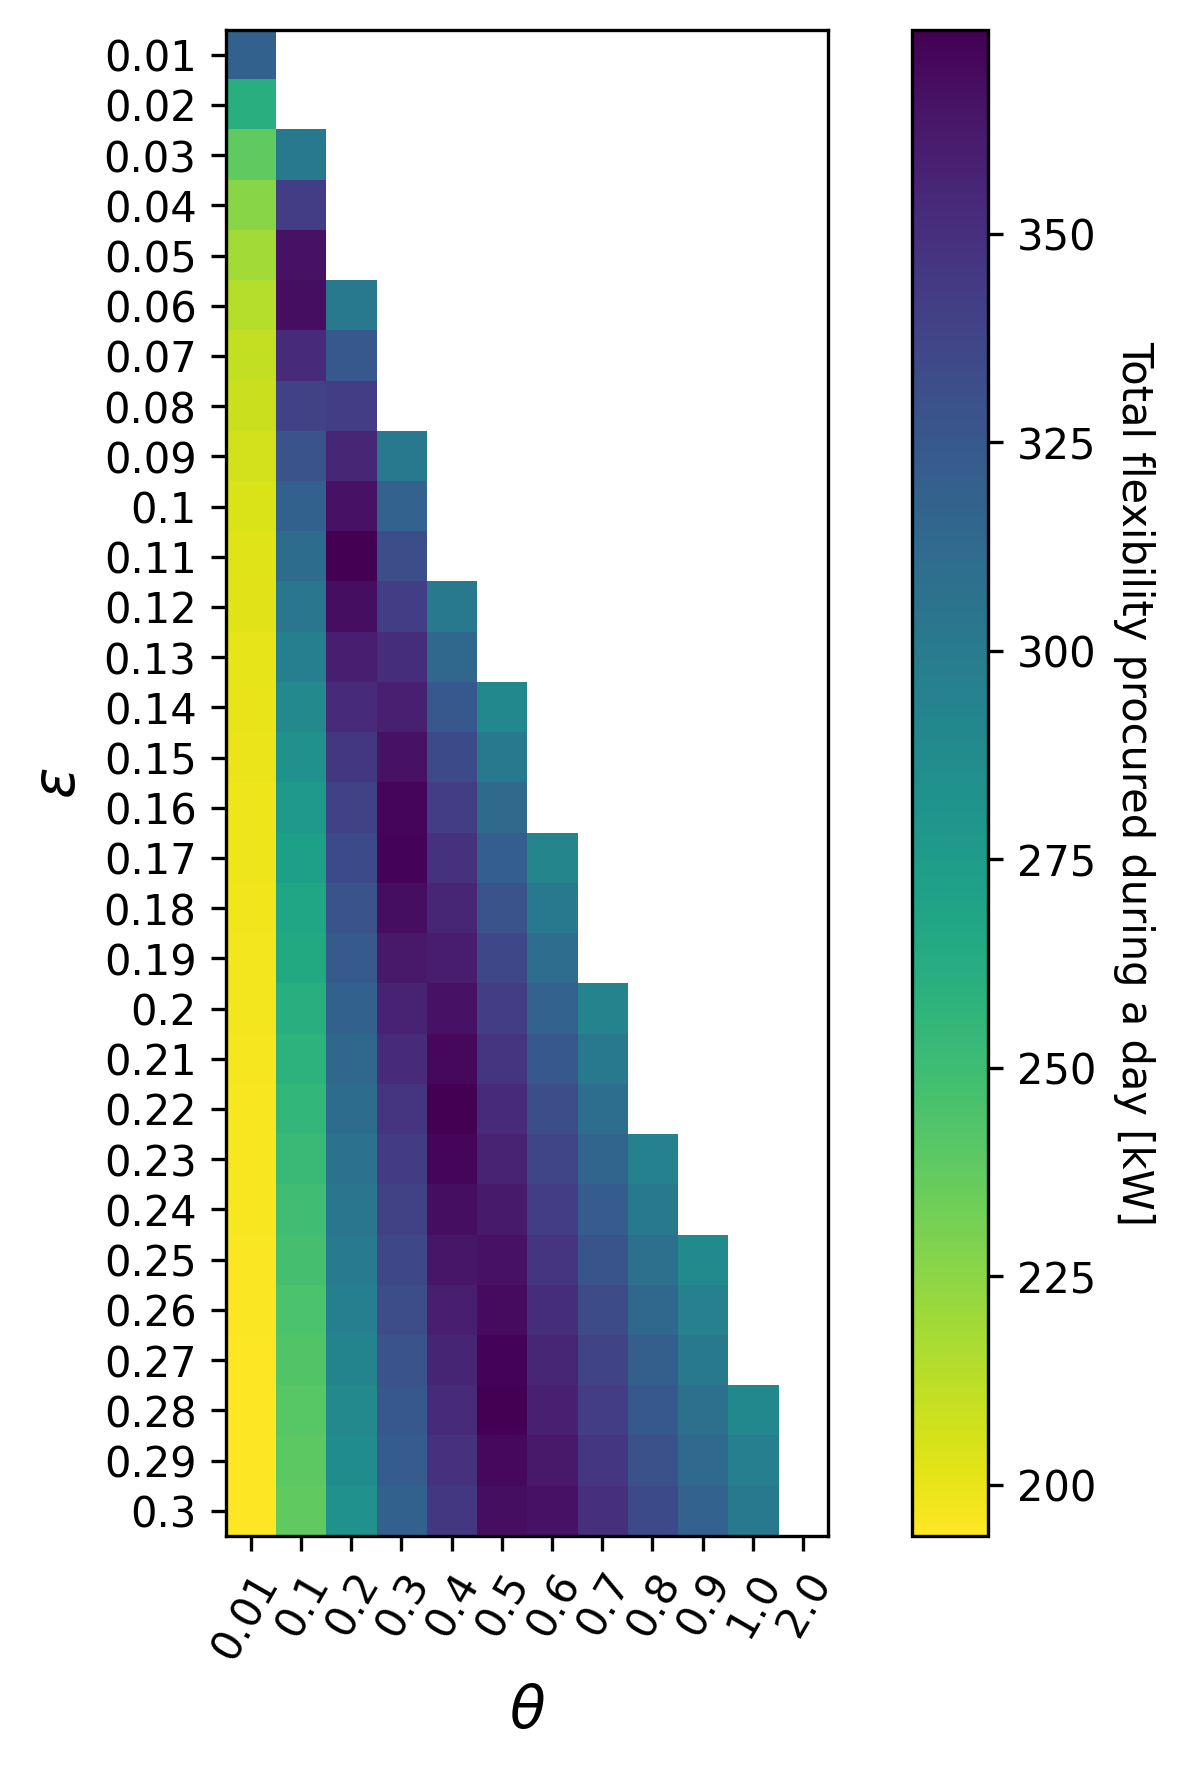
\includegraphics[width=0.95\columnwidth]{../figures/heatmap.png}
    \caption{\ac{TSO} flexibility procurement for given $\epsilon$ and $\theta$. Each $(\epsilon, \theta)$ has been solved using \eqref{P90:TSO} in a grid search on \ac{IS} data (see \ref{sec:sim-setup}). The optimal value is $(\epsilon, \theta) = (0.28, 0.5)$. }
    \label{fig:tso}
\end{figure}


\section{Conclusion}

This paper illustrated how stochastic flexible resources can participate in Nordic ancillary service markets using a \ac{DRJCCP} for offering capacity. We showed how a tractable formulation of the \ac{DRJCC} formulation allows for more robust bidding in non-stationary environments of the uncertain baseline power consumption. Furthermore, the perspective of the \ac{TSO} was also investigated with respect to its capacity procurement from such flexible resources. It was shown how an increased violation frequency, i.e., P90 level, should be offset by a corresponding increase in conservativeness of bidding using the measure of the Wasserstein distance in the \ac{DRJCC}. These findings were exemplified using a simulated case study of an aggregator of \acp{EV} bidding their flexibility into an ancillary service with negligible energy delivery.

For future work, it is of great interest to investigate the impact of a heterogenous portfolio of stochastic flexible resources with respect to \ac{TSO} procurement. As such, one could expect that flexible resources of different technology also respond differently when the \ac{TSO} prescribe violation frequencies and conservativeness. Moreover, our \ac{TSO} procurement in this work ignored prices, both for bids but also penalty prices for lack of capacity that was promised. Both are important from a system and societal perspective and should be included in future work. Lastly, an increase in supply of flexible resources lowers prices as well which will be offset by more uncertain supply. This trade-off is very interesting from a \ac{TSO} perspective, and should be studied further.


% \section*{Acknowledgement}

% The authors would like to thank...

\bibliographystyle{IEEEtran}

\bibliography{tex/bibliography/Bibliography}
%\bibliography{../bibliography/Bibliography}


\vfill

\end{document}
